\documentclass[11pt,oneside]{book}
\usepackage{fontspec}
\setmainfont{Noto Serif}
\setsansfont{Noto Sans}
\setmonofont{Noto Sans Mono}
\newfontfamily\proseunicodefont{DejaVu Serif}
\usepackage[margin=1in]{geometry}
\usepackage{microtype}
\usepackage{amsmath,amssymb,amsthm,mathtools,bm}
\usepackage{graphicx}
\usepackage{xcolor}
\usepackage{booktabs}
\usepackage{array}
\usepackage{longtable}
\usepackage{enumitem}
\usepackage{float}
\usepackage{caption}
\usepackage{hyperref}
\usepackage{fancyhdr}
\usepackage{tikz}
\usetikzlibrary{arrows.meta,positioning,calc,decorations.pathmorphing}

\hypersetup{
  colorlinks=true,
  linkcolor=blue!50!black,
  urlcolor=blue!50!black,
  citecolor=blue!50!black
}

\setlength{\parskip}{0.5em}
\setlength{\parindent}{0pt}
\setlist[itemize]{topsep=0.25em,itemsep=0.2em}
\setlist[enumerate]{topsep=0.25em,itemsep=0.2em}
\setlength{\headheight}{40pt}
\numberwithin{equation}{chapter}

\newtheorem{theorem}{Satz}[chapter]
\newtheorem{proposition}[theorem]{Proposition}
\newtheorem{lemma}[theorem]{Lemma}
\newtheorem{corollary}[theorem]{Korollar}
\theoremstyle{definition}
\newtheorem{definition}[theorem]{Definition}
\newtheorem{example}[theorem]{Beispiel}
\theoremstyle{remark}
\newtheorem{remark}[theorem]{Bemerkung}

\providecommand{\ket}[1]{\left\lvert#1\right\rangle}
\providecommand{\bra}[1]{\left\langle#1\right\rvert}
\providecommand{\braket}[2]{\left\langle#1\,\middle|\,#2\right\rangle}
\providecommand{\expect}[1]{\left\langle#1\right\rangle}
\newcommand{\lectureoverview}[1]{\paragraph{Überblick.} #1}

\makeatletter
\newcommand{\course@headerfont}{\normalfont\small\itshape}
\newcommand{\course@pagefont}{\normalfont\small}
\newcommand{\course@headerraise}{14pt}
\newlength{\course@headerboxheight}
\setlength{\course@headerboxheight}{\dimexpr\headheight-\course@headerraise-9pt\relax}
\newcommand{\course@leftheadbox}[1]{%
  \raisebox{\course@headerraise}{%
    \parbox[t][\course@headerboxheight][t]{0.82\textwidth}{%
      \raggedright\course@headerfont\strut\MakeUppercase{#1}\strut%
    }%
  }%
}
\newcommand{\course@rightheadbox}[1]{%
  \raisebox{\course@headerraise}{%
    \parbox[t][\course@headerboxheight][t]{0.82\textwidth}{%
      \raggedleft\course@headerfont\strut\MakeUppercase{#1}\strut%
    }%
  }%
}
\renewcommand{\chaptermark}[1]{\markboth{\MakeUppercase{\chaptername\ \thechapter.\ #1}}{}}
\renewcommand{\sectionmark}[1]{\markright{\MakeUppercase{\thesection\hspace{0.4em}#1}}}
\fancyhf{}
\fancyhead[L]{\course@leftheadbox{\leftmark}}
\fancyhead[R]{\course@pagefont\thepage}
\renewcommand{\headrulewidth}{0.5pt}
\pagestyle{fancy}
\fancypagestyle{plain}{%
  \fancyhf{}
  \fancyhead[L]{\course@leftheadbox{\leftmark}}
  \fancyhead[R]{\course@pagefont\thepage}
  \renewcommand{\headrulewidth}{0.5pt}
}
\makeatother

% Reader-facing provenance for classroom exchanges and editorial additions.
\newenvironment{classroomqa}{%
  \par\medskip\noindent\begin{minipage}{\linewidth}\small\hrule\medskip
}{%
  \medskip\hrule\end{minipage}\par\medskip
}
\newcommand{\audiencequestion}[1]{\noindent\textbf{Frage aus dem Publikum.} #1\par\smallskip}
\newcommand{\lecturerresponse}[1]{\noindent\textbf{Antwort.} #1\par}
\newcommand{\lecturetimestamp}[1]{\footnote{Vorlesungszeit: #1.}}
\newcommand{\lectureframe}[1]{\par\smallskip{\centering\footnotesize\itshape Vorlesungsbild: #1.\par}}
\newcommand{\editorialnote}[1]{\footnote{Redaktionelle Klarstellung: #1}}

\usepackage{polyglossia}
\setdefaultlanguage{german}
\usepackage{sectsty}
\renewcommand{\contentsname}{Inhaltsverzeichnis}
\renewcommand{\chaptername}{Kapitel}
\renewcommand{\figurename}{Abbildung}
\renewcommand{\tablename}{Tabelle}
\renewcommand{\proofname}{Beweis}
\renewcommand{\bibname}{Literatur}
\sectionfont{\raggedright}
\subsectionfont{\raggedright}
\makeatletter
\renewcommand{\@pnumwidth}{2.2em}
\renewcommand{\@tocrmarg}{3.2em}
\makeatother
\usepackage{tocloft}
\renewcommand{\cftchapfont}{\small\bfseries}
\renewcommand{\cftchappagefont}{\small\bfseries}
\renewcommand{\cftsecfont}{\small}
\renewcommand{\cftsecpagefont}{\small}
\setlength{\cftsecnumwidth}{3em}
\renewcommand{\cftsubsecfont}{\small}
\renewcommand{\cftsubsecpagefont}{\small}
\setlength{\cftsubsecindent}{4.5em}
\setlength{\cftsubsecnumwidth}{4em}
\emergencystretch=6em
\pdfstringdefDisableCommands{\def\proseunicodefont{}}

\geometry{paperwidth=177.6mm,paperheight=252mm,left=16mm,right=16mm,
 top=18mm,bottom=18mm,includeheadfoot,headheight=28pt,headsep=7mm,footskip=9mm}
\usepackage{scrextend}
\changefontsizes[17pt]{12pt}
\raggedbottom
\renewenvironment{classroomqa}{\par\medskip\begingroup}{\par\endgroup\medskip}
\fancyhf{}
\setlength{\headwidth}{\textwidth}
\fancyhead[L]{\parbox{\textwidth}{\raggedright\fontsize{9}{11}\selectfont\nouppercase{\leftmark}}}
\fancyfoot[C]{\small\thepage}
\renewcommand{\headrulewidth}{0.3pt}
\fancypagestyle{plain}{\fancyhf{}\fancyfoot[C]{\small\thepage}\renewcommand{\headrulewidth}{0pt}}

\hypersetup{
  pdftitle={Topics in String Theory},
  pdfauthor={Leonard Susskind},
  pdfsubject={Independently edited companion notes for the 2011 Winter lecture course},
  pdfcreator={LaTeX with hyperref}
}
\graphicspath{{../../../generated_course_notes/supplementary/cosmology_and_black_holes/2011_winter_topics_in_string_theory/figures/}{../../../generated_course_notes/supplementary/cosmology_and_black_holes/2011_winter_topics_in_string_theory/assets/}}
\begin{document}
\frontmatter
\hypersetup{pageanchor=false}
\begin{titlepage}
\hyphenpenalty=10000\exhyphenpenalty=10000
\thispagestyle{empty}
\begin{tikzpicture}[remember picture,overlay]
  \node[anchor=center,inner sep=0] at (current page.center) {%
    \includegraphics[height=\paperheight,keepaspectratio]{../../../generated_course_notes/supplementary/cosmology_and_black_holes/2011_winter_topics_in_string_theory/assets/cover-art.png}%
  };
  \node[
    anchor=north west,
    align=left,
    text width=0.78\paperwidth,
    fill=white,
    fill opacity=0.9,
    rounded corners=8pt,
    inner xsep=10pt,
    inner ysep=8pt
  ] at ([xshift=0.08\paperwidth,yshift=-0.06\paperheight]current page.north west) {%
    {\fontsize{30}{33}\selectfont\bfseries\color{black!88} Themen der Stringtheorie\\[0.85em]}
    {\large\color{black!72} Deutsche Ausgabe / Winter 2011, Themen der Stringtheorie}
  };
  \node[
    anchor=south west,
    align=left,
    text width=0.68\paperwidth,
    fill=white,
    fill opacity=0.82,
    text opacity=1,
    rounded corners=6pt,
    inner sep=12pt
  ] at ([xshift=0.08\paperwidth,yshift=0.08\paperheight]current page.south west) {%
    {\normalsize\color{black!78} Originalvorlesungen: Leonard Susskind\\[0.35em]}
    {\small\color{black!72} Begleitausgabe: \href{https://lazying.art}{LazyingArt LLC} / \href{https://github.com/lachlanchen/Video2Book}{Video2Book}}
  };
\end{tikzpicture}
\mbox{}
\end{titlepage}
\hypersetup{pageanchor=true}

\clearpage
\chapter*{Über diese Notizen}
Diese unabhängig redigierten Begleitnotizen folgen den Vorlesungen von Leonard Susskind. Sie wurden anhand maschineller Transkripte, Untertitel und ausgewählter Tafelbilder rekonstruiert und anschließend mit dem verfügbaren Quellenmaterial abgeglichen. Sie sind kein Originalmanuskript von Professor Susskind und wurden von ihm weder geprüft noch gebilligt.

Die Ausgabe wurde von \href{https://lazying.art}{LazyingArt LLC} mithilfe des Open-Source-Toolkits \href{https://github.com/lachlanchen/Video2Book}{Video2Book} erstellt. Maschinelle Transkripte sind separat verfügbar und können Erkennungsfehler enthalten. Redaktionelle Klarstellungen und nicht triviale Rekonstruktionen sind in Fußnoten gekennzeichnet.
\clearpage
\tableofcontents
\mainmatter
\chapter{Vorlesung 1: Themen der Stringtheorie}

\lectureoverview{Die Herausforderung des Reduktionismus wird durch die Bosonisierung in \(1+1\) Dimensionen, die elektrische--magnetische Dualität, D-Branen, Übergänge bei starker Kopplung, emergente Geometrie und die kombinatorische Landschaft der Stringvakuua zugespitzt. Dasselbe physikalische System kann sehr unterschiedliche elementare Beschreibungen zulassen; welche davon einfach erscheint, hängt von der Kopplung und der Geometrie ab.}

\section{Reduktionismus, Komplexität und die Frage nach der Einfachheit}

Susskind beginnt mit einem bewusst vertrauten philosophischen Slogan: Große Dinge bestehen aus kleinen Dingen, und kleine Dinge aus noch kleineren. Dann fügt er die anspruchsvollere Fassung desselben Gedankens hinzu, auf die es für die fundamentale Physik wirklich ankommt: Wenn man zu tieferen Schichten vordringt, sollten die Objekte nicht nur kleiner, sondern auch einfacher werden. Sein Bild: Häuser bestehen aus Ziegeln, und niemand verwechselt ein Haus mit einem Ziegel. Der Ziegel ist kleiner, aber auch einfacher.

Als ersten Schritt konfrontiert die Vorlesung diese Erwartung mit dem tatsächlichen Stand der Teilchenphysik. Würde der Reduktionismus in diesem starken Sinn zu wachsender Einfachheit führen, könnte man erwarten, dass die heutige Elementarteilchenphysik überschaubar wäre. Stattdessen betont Susskind, dass die Bestandsaufnahme schon vor Einbeziehung der Quantengravitation unübersichtlich aussieht. Die Zahlen in der Vorlesung sind grobe Schätzungen, doch gerade das gehört zum Argument:
\begin{equation}
\begin{aligned}
N_{\mathrm{species}}&\sim 75,\\
N_{\mathrm{independent}}&\sim 10\text{--}20,\\
N_{\mathrm{parameters}}&\sim 20.
\end{aligned}
\end{equation}
Damit ist die Geschichte noch nicht zu Ende. Das Standardmodell enthält keine Gravitation, erklärt die Dunkle Materie nicht, liefert nicht die für die Inflation erforderliche zusätzliche Struktur und weist ein gravierendes Feinabstimmungsproblem auf. Die üblichen Lösungsansätze erhöhen die Zahl nur weiter. Als Beispiel nennt die Vorlesung die Supersymmetrie. Zur Zeit der Vorlesung hofften viele Physiker, der Large Hadron Collider werde Superpartner nachweisen. Susskind betont, dass die entsprechende Erweiterung die Bestandsaufnahme um mehr als hundert zusätzliche Parameter vergrößern würde, statt sie unmittelbar zu vereinfachen. Seine schematische Aussage lautet:
\begin{equation}
N_{\mathrm{parameters}}^{\mathrm{extended}} \sim 200.
\end{equation}
Diese Zahlen sind bewusst grob und an den damaligen Stand gebunden. Sie veranschaulichen das Argument, dass eine tiefere Beschreibung hinsichtlich ihres Teilchenbestands und ihrer gemessenen Konstanten nicht unbedingt einfacher aussehen muss.

Diese quantitative Kritik ist noch nicht Susskinds Hauptthese, sondern deren Vorbereitung. Die weitergehende Behauptung, die den Rest der Vorlesung bestimmt, lautet, dass die moderne Quantenfeldtheorie und die Stringtheorie keine eindeutige, von der Kopplung unabhängige Unterscheidung zwischen Ziegeln und Häusern nahelegen. Die folgenden Beispiele sollen zeigen, dass die Bedeutung von ``elementar'' davon abhängen kann, welche Variablen sich effizient verwenden lassen.

\section{Bosonisierung: Ein erstes Aufbrechen fester Fundamentalität}

Susskinds erstes theoretisches Beispiel stammt aus einer Quantenfeldtheorie in \(1+1\) Dimensionen: einer Raum- und einer Zeitdimension. Gleich zu Beginn kündigt er an, dass er die Äquivalenz nicht im Einzelnen herleiten wird; es gehe nicht um den formalen Beweis, sondern um die begriffliche Einsicht.

Ausgangspunkt ist eine Feldtheorie von Fermionen. Das Fermionfeld wird mit \(\psi\) bezeichnet. Zwei nahe beieinanderliegende Fermionen können einen bosonischen Verbund bilden; das zugehörige Bosonenfeld wird mit \(\phi\) bezeichnet. Auf den ersten Blick scheint die Hierarchie klar: \(\psi\) ist fundamental, während \(\phi\) eine zusammengesetzte oder effektive Variable ist. In der Vorlesung wird das Boson genau so eingeführt: als Feld, das gebundene Fermionenpaare erzeugt.

Es stellte sich jedoch heraus, dass sich dieselbe Theorie mit umgekehrtem Ausgangspunkt formulieren lässt. Man kann mit dem Bosonenfeld \(\phi\) beginnen; dann erscheint das Fermion nicht mehr als punktförmiger Bestandteil. Stattdessen tritt es als Knick des Bosonenfeldes auf, als ausgedehnte Konfiguration, in der \(\phi\) glatt zwischen zwei asymptotischen Werten interpoliert. Der minimale mathematische Inhalt der Vorlesung ist diese asymptotische Struktur:
\begin{equation}
\phi(x\to -\infty)=\phi_-,
\qquad
\phi(x\to +\infty)=\phi_+.
\end{equation}
Eine zweckmäßige schematische Darstellung ist
\begin{equation}
\phi(x)\approx \frac{\phi_++\phi_-}{2}
+
\frac{\phi_+-\phi_-}{2}\tanh\!\left(\frac{x}{\ell}\right),
\end{equation}
Dabei bezeichnet \(\ell\) die Breite des Übergangsbereichs.

\editorialnote{Das Hyperbeltangens-Profil ist eine übliche glatte Darstellung des in der Vorlesung skizzierten Knicks, keine dort hergeleitete Formel. Die genaue Bosonisierungszuordnung hängt vom Modell ab; entscheidend ist der begriffliche Austausch zwischen einer fermionischen Anregung und einem topologischen Soliton eines Bosonenfeldes.}

Die Gürtelanalogie der Vorlesung ist anschaulich genug, um sie beizubehalten. Ein flach liegender, unverdrehter Gürtel entspricht einer Konfiguration ohne Knick. Dreht man ein Ende um \(2\pi\), hat der Gürtel weit entfernt wieder dieselbe lokale Ausrichtung, muss dazwischen aber einen ausgedehnten verdrehten Bereich durchlaufen. Dieser verdrehte Bereich ist der Knick. In der bosonischen Beschreibung wird das Fermion genau durch ein solches ausgedehntes Objekt dargestellt.

Mit der Einführung einer Kopplung wird der Punkt deutlicher. Susskind bezeichnet sie in diesem Beispiel mit \(G\). Die Aussage lautet nicht bloß, dass die beiden Beschreibungen irgendwie zusammenhängen, sondern dass ihre Effizienz vom Parameterbereich abhängt:
\begin{align}
G \ll 1
&\Rightarrow
\ell\text{ small, tight kink; }\psi\text{ efficient},\\
G \gg 1
&\Rightarrow
\ell\text{ large, broad kink; }\phi\text{ efficient}.
\end{align}
Für kleine Werte von \(G\) ist der Knick schmal und das Fermion erscheint als einfaches Objekt. Mit zunehmendem \(G\) wird der Knick breiter und das Fermion weniger punktförmig. Dann sind die bosonischen Variablen die sparsamere Beschreibung.

\paragraph{Schematischer Ablauf.}
\begin{enumerate}
\item Ausgangspunkt ist eine fermionische Theorie, beschrieben durch \(\psi\).
\item Bosonische Verbünde identifizieren, beschrieben durch \(\phi\).
\item Dieselbe Theorie vollständig in Termen von \(\phi\) umformulieren.
\item In der bosonischen Beschreibung tritt das Fermion als Knick der Breite \(\ell\) wieder auf.
\item Für \(G\ll 1\) ist \(\ell\) klein und die fermionische Beschreibung am einfachsten.
\item Bei größerem \(G\) wächst \(\ell\), und die bosonische Beschreibung wird am einfachsten.
\end{enumerate}

Dies ist das erste ausdrückliche Gegenbeispiel zum festen Bild von ``Häusern und Ziegeln''. Die Pointe der Vorlesung ist nicht bloß, dass zusammengesetzte Objekte existieren, sondern dass sich je nach Kopplung ändern kann, welche Variable als elementar gilt.

\section{Elektrische Ladung, magnetische Monopole und schwache gegenüber starker Kopplung}

Als Nächstes fragt Susskind, ob sich eine ähnliche Geschichte auch in der vertrauteren Teilchenphysik findet. Sein Beispiel ist der Gegensatz zwischen elektrischer Ladung und magnetischem Monopol. Ein gewöhnliches geladenes Teilchen wie das Elektron ist in dieser Sprache ein elektrischer Monopol: eine lokalisierte Quelle eines elektrischen Feldes. Der magnetische Monopol wird anhand eines Stabmagneten eingeführt. Könnte man das Ende eines Stabmagneten irgendwie isolieren, ohne den unsichtbaren verbindenden Stab, sähen die Feldlinien genauso aus wie die eines elektrischen geladenen Teilchens, wären aber magnetischer statt elektrischer Natur.

Der maßgebliche Kontrollparameter ist die Feinstrukturkonstante \(\alpha\). In der Vorlesung behandelt Susskind sie heuristisch als Quadrat der elektrischen Ladung:
\begin{equation}
\alpha \sim e^2.
\end{equation}
Außerdem gibt er eine grobe operationale Deutung: Sie misst, wie leicht ein Elektron Strahlung emittiert. Die Stärke fasst er so zusammen, dass ein beschleunigtes Elektron in dem hier gemeinten Sinn Photonen in einer Größenordnung von ``\(1/100\)'' abstrahlt. In der groben numerischen Sprache der Vorlesung:
\begin{equation}
\alpha \approx 10^{-2}.
\end{equation}
Das ist nicht als präzise Konvention gedacht, sondern als didaktische Möglichkeit auszudrücken, dass die elektrische Ladung schwach ist.

\editorialnote{Der Zusammenhang zwischen schwacher--starker Kopplung hat einen präzisen Vorläufer in der Dirac-Quantisierung. In einer verbreiteten Konvention erfüllen elektrische und magnetische Ladungen die Beziehung \(e g_m=2\pi n\). Eine schwache elektrische Kopplung entspricht damit einer starken magnetischen, auch wenn genaue numerische Faktoren und geschützte Massenbeziehungen von der Theorie abhängen.}

Für \(\alpha\ll 1\) ist das Elektron das einfache Objekt. Sein elektrisches Feld ist schwach, seine Vakuumpolarisationswolke dünn, und es erscheint nahezu punktförmig. Beim magnetischen Monopol ist es umgekehrt: Sein Feld ist enorm, seine Umgebung stark verzerrt, und er ist ausgedehnt, kompliziert und schwer. Susskind fasst die Lage genau in diesem Stil schwacher--starker Kopplung zusammen:
\begin{equation}
\begin{aligned}
\alpha \ll 1
&\Rightarrow \text{simple electron;}\\
&\phantom{\Rightarrow{}}\text{heavy, extended monopole},\\
\alpha \gg 1
&\Rightarrow \text{simple monopole;}\\
&\phantom{\Rightarrow{}}\text{heavy, structured electron}.
\end{aligned}
\end{equation}
Die Vorlesung leitet keine Massenformel für den Monopol her; das ist auch nicht nötig. Entscheidend ist die qualitative Aussage. Mit zunehmendem \(\alpha\) wird das Feld des Elektrons stärker und seine Struktur wächst, während der Monopol schrumpft und leichter wird. Weit oberhalb der Einheit kehrt sich die zweckmäßigste Beschreibung um: Der Monopol ist einfach und das Elektron kompliziert.

Das ist die feldtheoretische Fassung der früheren Einsicht aus der Bosonisierung. Die Unterscheidung zwischen fundamental und zusammengesetzt ist nicht absolut, sondern hängt von der Kopplung ab.

\begin{classroomqa}\audiencequestion{Wenn der Reduktionismus kein verlässlicher Wegweiser ist, warum verlassen sich Physiker dann auf die Infinitesimalrechnung, die ein System scheinbar in beliebig kleine Teile zerlegt? \lecturetimestamp{00:21:21}}\lecturerresponse{Die Infinitesimalrechnung beschreibt glatte Veränderungen; sie legt nicht fest, welche Objekte in einer Theorie fundamental sind. Quantenfelder fluktuieren auf jeder Längenskala. So entsteht eine endlose Hierarchie statt einer letzten glatten Schicht, auf der sich ein für alle Mal entscheiden ließe, was elementar ist.}\end{classroomqa}

Die Diskussion geht mit dem Vorschlag weiter, die Hierarchie ähnele einem Fraktal. Susskind stimmt der Analogie zu und präzisiert sie dann: Quantenfelder fluktuieren auf jeder Skala und sind daher im klassischen Sinn niemals glatt. Diese übermäßigen Schwankungen tragen zur mathematischen Schwierigkeit der Quantenfeldtheorie bei; die gewöhnliche Infinitesimalrechnung muss mit renormierten Größen arbeiten und nicht mit einem naiv glatten mikroskopischen Feld.

\section{Strings, D-Branen und die Rückkehr der Dualität zwischen schwacher--starker Kopplung}

Der nächste Übergang in der Vorlesung ist bewusst naiv. Wenn die Stringtheorie die Theorie der fundamentalen Bausteine sein soll, dann muss die Antwort doch einfach sein: Die Bausteine sind Strings. Susskind spricht diese Erwartung ausdrücklich aus und verwendet dann den nächsten Teil der Vorlesung darauf, sie zu erschüttern.

\subsection{Warum Strings nicht die ganze Geschichte sind}

Die erste Komplikation ist die unvermeidliche Existenz von D-Branen. Eine D\(p\)-Brane ist ein Objekt mit \(p\) Dimensionen, an dem Strings enden können. Der Buchstabe \(D\) geht auf Dirichlet-Randbedingungen zurück, doch der Name ist weit weniger wichtig als die Funktion: Diese Objekte gehören zur Theorie und lassen sich nicht weglassen. Sie sind keine optionalen Verzierungen.

Die einfachsten Beispiele sind:
\begin{itemize}
\item eine D0-Brane, die punktförmig ist,
\item eine D1-Brane oder ein D-String, der stringartig ist,
\item ein F-String, der gewöhnliche fundamentale String.
\end{itemize}
Eine D0-Brane ist ein schwerer, punktförmiger Ort, an dem beliebig viele F-Strings enden können. Eine D1-Brane ist ein schweres, kabelartiges Objekt, das deutlich dicker ist und mehr Masse pro Längeneinheit besitzt als ein F-String, aber ebenfalls Endpunkte für F-Strings bietet. Bei schwacher Kopplung stellt die Vorlesung diese Objekte nicht als gleichwertige elementare Alternativen dar. D-Branen werden als schwere, strukturierte, zusammengesetzt wirkende Objekte eingeführt, die uns die Theorie dennoch aufzwingt.

\editorialnote{Die in diesem Teil der Vorlesung verwendete Theorie mit ungeraden Branen ist die Stringtheorie vom Typ IIB. Ihre stabilen D-Branen haben ungerade räumliche Dimensionen, darunter D1- und D3-Branen. Susskind schiebt diese Bezeichnungen auf, weil zunächst das Dualitätsmuster und nicht die Taxonomie im Mittelpunkt steht.}

\paragraph{Notation.}
Susskind verwendet \(G\) und \(g\) in verschiedenen Teilen der Vorlesung nicht ganz einheitlich. Hier steht \(G\) für das Bosonisierungsbeispiel, während \(g\) die Stringkopplung bezeichnet.

Die Stringkopplung \(g\) wird operational definiert, nicht axiomatisch. Sie ist der Parameter, der die Wahrscheinlichkeit dafür angibt, dass ein fluktuierender String aufspaltet und Tochterstrings bildet. Deshalb vergleicht Susskind ihre Rolle unmittelbar mit der von \(\alpha\) in der Quantenelektrodynamik. Außerdem hält die Vorlesung kurz fest, dass die Spannung der Energie pro Längeneinheit entspricht:
\begin{equation}
T=\frac{E}{L}=\frac{M}{L}.
\end{equation}

Für einen F-String und einen D-String machen die üblichen Spannungsformeln den Vergleich zwischen schwacher--starker Kopplung ausdrücklich:
\begin{equation}
T_{\mathrm{F1}}=\frac{1}{2\pi\alpha'},
\qquad
T_{\mathrm{D1}}=\frac{1}{2\pi\alpha' g_s},
\qquad
\frac{T_{\mathrm{D1}}}{T_{\mathrm{F1}}}=\frac{1}{g_s}.
\end{equation}
\editorialnote{Diese Spannungsformeln liefern die übliche Normierung für den qualitativen Vergleich von Kabel und Faden in der Vorlesung. Sie wurden redaktionell ergänzt; in der Vorlesung wird nur die Skalierung mit der Kopplung verwendet.}

\subsection{F-Strings und D-Strings}

Das Muster schwacher--starker Kopplung wiederholt sich nun in der Sprache der Stringtheorie. Bei kleiner Kopplung ist der F-String leicht und dünn und entspricht weitgehend dem ursprünglichen anschaulichen Bild eines fundamentalen Objekts. Der D-String ist dick, schwer und voller F-String-Struktur. Mit wachsender Kopplung spaltet sich der F-String leichter auf; die Wolke aus Tochterstrings um ihn herum wird dichter, und er wird schwerer und komplizierter. Gleichzeitig fällt es dem D-String zunehmend schwer, die nun schweren F-Strings zu emittieren. Seine umgebende Struktur lichtet sich, und er wird leichter und linienartiger. Die Zuordnung schwacher--starker Kopplung in der Vorlesung lautet daher:
\begin{align}
g \ll 1
&\Rightarrow
\begin{gathered}
\text{F-string light and thin;}\\
\text{D-string heavy and structured},
\end{gathered}\\
g \sim 1
&\Rightarrow
\text{F-string and D-string comparable},\\
g \gg 1
&\Rightarrow
\begin{gathered}
\text{D-string light and thin;}\\
\text{F-string heavy and structured}.
\end{gathered}
\end{align}
Susskind merkt an, dass die beiden Beschreibungen bei \(g\sim 1\) nicht mehr klar voneinander zu unterscheiden sind. Jenseits dieses Punktes tauschen sie im Wesentlichen ihre Rollen. Das ist die stringtheoretische Variante des Austauschs zwischen Elektron und Monopol--; sie wird als S-Dualität bezeichnet.

Derselbe Austausch lässt sich auch verfolgen, wenn ein String sich zu einer Schleife schließt. Bei schwacher Kopplung ist eine kleine F-String-Schleife eine leichte, teilchenartige Anregung, während die entsprechende D-String-Schleife schwer und kompliziert ist. Bei starker Kopplung kehren sich ihre Rollen um: Die D-String-Schleife wird zur leichten Beschreibung, und zu den daraus hervorgehenden leichten geschlossenen Stringanregungen gehört das Graviton. Mit diesem Beispiel unterstreicht die Vorlesung, dass sogar die Identität eines vertrauten Teilchens davon abhängen kann, welche Seite der Dualität man verwendet.

Die Vorlesung führt den Gedanken noch einen Schritt weiter. In der idealisierten Theorie ist die Kopplung nicht einfach eine von Hand einstellbare Zahl, sondern verhält sich wie ein Feld. Schematisch:
\begin{equation}
g = g(x).
\end{equation}
Daher können in verschiedenen Raumbereichen unterschiedliche Dualitätsbeschreibungen zweckmäßig sein. In einem Bereich sind F-Strings die leichten Variablen, in einem anderen D-Strings. Dazwischen ist keine der beiden Beschreibungen besonders einfach. Deshalb stellt die Stringtheorie für Susskind das einfache reduktionistische Bild nicht wieder her, sondern verschärft die Mehrdeutigkeit.

\editorialnote{In der perturbativen Stringtheorie wird die lokale Kopplung durch das Dilaton \(g_s(x)=e^{\Phi(x)}\) bestimmt. Die Schreibweise \(g=g(x)\) ist daher mehr als eine Analogie, auch wenn realistische Kompaktifizierungen im Allgemeinen ein Potential erzeugen, das solche Variationen einschränkt.}

\begin{classroomqa}\audiencequestion{Wenn die Kopplung so stark variierte, dass D-Strings in einem anderen Bereich leichter als F-Strings würden, würde sich das auf beobachtbare Spektren auswirken? \lecturetimestamp{00:34:15}}\lecturerresponse{Ja. Das ist einer der Gründe, warum sich das hier betrachtete, exakt symmetrische und mathematisch kontrollierbare Modell nicht unmittelbar mit unserer Welt gleichsetzen lässt. Es geht um das, was konsistente Quantentheorien leisten können, nicht um ein wörtliches Spektrum der Natur.}\end{classroomqa}

\begin{classroomqa}\audiencequestion{Gibt es eine analoge duale Beschreibung für eine D2-Brane? \lecturetimestamp{00:34:39}}\lecturerresponse{Ja, aber es handelt sich nicht um einen weiteren Austausch nach Art der D-Strings. Der Fall geradzahliger Branen führt zu einer Interpretation durch Membranen und zu einer zusätzlichen Raumdimension; das ist die nächste Konstruktion.}\end{classroomqa}

\begin{classroomqa}\audiencequestion{Erklärt eine höhere Aufspaltungswahrscheinlichkeit der Strings die zunehmende innere Komplexität? \lecturetimestamp{00:34:53}}\lecturerresponse{Ja. Um den Mechanismus anschaulich zu machen, kehren wir zur Quantenelektrodynamik zurück: Ein Elektron emittiert Photonen, Photonen fluktuieren zu geladenen Paaren, und diese geladenen Linien strahlen ihrerseits wieder. Bei stärkerer Kopplung wird diese Hierarchie dichter.}\end{classroomqa}

\subsection{Rückkehr zur Quantenelektrodynamik ausgehend von einer Frage}

Ein Student fragt daraufhin, ob die höhere Aufspaltungswahrscheinlichkeit schlicht eine kompliziertere Struktur ``weiter oben'' bedeutet. Susskind antwortet, indem er zur Quantenelektrodynamik zurückkehrt und erneut die Weltlinie des Elektrons zeichnet. Diese Rückkehr ist wichtig: Sie zeigt, dass die Stringgeschichte keine isolierte Kuriosität ist, sondern ein weiteres Beispiel desselben Musters schwacher--starker Kopplung.

\begin{figure}[htbp]\centering
\begin{tikzpicture}[scale=1.0]
\draw[->] (-1.2,0) -- (3.7,0) node[right] {space};
\draw[->] (0,-0.2) -- (0,4.3) node[above] {time};

\draw[line width=0.9pt] (0,0.2) -- (0,4.0);
\node[left] at (0,3.55) {\(e^{-}\)};

\draw[line width=0.8pt] (0,1.0) -- (0.18,1.08) -- (0.36,0.92) -- (0.54,1.10) -- (0.72,0.94) -- (0.90,1.12) -- (1.08,0.96) -- (1.26,1.14);
\draw[line width=0.8pt] (0,2.35) -- (-0.18,2.43) -- (-0.36,2.27) -- (-0.54,2.45) -- (-0.72,2.29) -- (-0.90,2.47);

\draw[line width=0.8pt] (1.26,1.14) -- (1.48,1.42);
\draw[line width=0.8pt] (1.26,1.14) -- (1.04,1.42);
\draw[line width=0.8pt] (1.48,1.42) -- (1.58,2.10);
\draw[line width=0.8pt] (1.04,1.42) -- (0.94,2.10);
\draw[line width=0.8pt] (0.94,2.10) -- (1.58,2.10);

\draw[line width=0.7pt] (1.58,1.78) -- (1.72,1.84) -- (1.86,1.72) -- (2.00,1.86);
\draw[line width=0.7pt] (0.94,1.78) -- (0.80,1.84) -- (0.66,1.72) -- (0.52,1.86);

\node at (2.35,1.95) {\(\gamma\)};
\node at (-1.15,2.75) {\(\gamma\)};
\end{tikzpicture}\caption{Schematische QED-Hierarchie aus der Vorlesung: Ein punktförmiges Elektron emittiert Photonen, Photonen erzeugen Paare, und die geladenen Tochterlinien strahlen erneut. So entsteht Struktur auf immer kleineren Skalen.}\end{figure}

Der Punkt der Vorlesung ist, dass selbst ein punktförmiges Elektron von einer Hierarchie von Prozessen begleitet wird:
\begin{enumerate}
\item Ein Elektron emittiert und absorbiert Photonen.
\item Ein Photon kann ein Elektron--Positron-Paar erzeugen.
\item Die geladenen Tochterlinien können selbst Photonen emittieren.
\item Die Hierarchie setzt sich auf immer kleineren Skalen fort.
\end{enumerate}
Bei schwacher Kopplung ist diese Wolke dünn, sodass das Elektron im Labor nahezu punktförmig erscheint. Bei stärkerer Kopplung wird sie dichter, und das Elektron entwickelt eine innere Struktur. Die Stringgeschichte wird als direkte Analogie dazu vorgestellt.

Dieselbe spätere Diskussion führt auch zu Susskinds heuristischer Energiebilanz. Er betont, dass die relevante Energie nicht bloß die Summe der Beiträge freier Teilchen ist. Auch die Wechselwirkungsenergie muss berücksichtigt werden:
\begin{equation}
E_{\mathrm{tot}} = E_e + E_\gamma + E_{\mathrm{int}}.
\end{equation}
Hier ist \(E_{\mathrm{int}}\) der entscheidende Term. Er ermöglicht es, in der Masse des „bekleideten“ Elektrons die Energie seines umgebenden Feldes und seiner virtuellen Struktur zu berücksichtigen. Die Vorlesung entwickelt daraus keine formale Herleitung einer renormierten Selbstenergie. Der Gedanke ist heuristisch, aber wesentlich: Die Masse des Objekts umfasst bereits die Wechselwirkungsenergie, die erforderlich ist, um die komplizierte Wolke um es herum aufrechtzuerhalten.

\begin{classroomqa}\audiencequestion{Woher stammt die Energie für virtuelle Photonen und Elektron--Positron-Paare, wenn ein Elektron nicht genügend freie Energie enthält, um ein reales Paar zu erzeugen? \lecturetimestamp{00:37:01}}\lecturerresponse{Man beginnt nie mit einem nackten Elektron und fügt ihm später sein Coulombfeld hinzu. Das beobachtete Elektron ist ein bekleideter Zustand, dessen Masse das Feld und die Wechselwirkungsenergie bereits umfasst. In der QED ist die Gesamtenergie nicht allein die Summe aus der Energie des freien Elektrons und der freien Photonen; der Wechselwirkungsterm ist unverzichtbar. Die Zwischenpaare als virtuell zu bezeichnen ist hilfreich, doch die Energiebilanz gehört zum vollständigen wechselwirkenden Zustand.}\end{classroomqa}

\begin{classroomqa}\audiencequestion{Erzeugt eine hochenergetische Sonde diese Struktur, wenn sie sie sichtbar macht, statt etwas bereits Vorhandenes zu entdecken? \lecturetimestamp{00:38:59}}\lecturerresponse{Diese Deutung lässt sich diskutieren. Operational betrachtet haben Streuprozesse bei hinreichend hoher Energie einen berechenbaren, nichttrivialen Endzustand. Bei schwacher Kopplung wirken die meisten Ereignisse weiterhin einfach, während ungefähr ein Anteil von der Größenordnung \(\alpha\) zusätzliche Strahlung oder Paare erkennen lässt.}\end{classroomqa}

\begin{classroomqa}\audiencequestion{Wenn die D1-Brane als massereicher als der F-String bezeichnet wird, ist dann auch ihre Spannung größer? \lecturetimestamp{00:39:37}}\lecturerresponse{Ja. Bei einem ausgedehnten String bedeutet ``Masse'' hier Energie pro Längeneinheit, also genau die Spannung.}\end{classroomqa}

\begin{figure}[htbp]
\centering
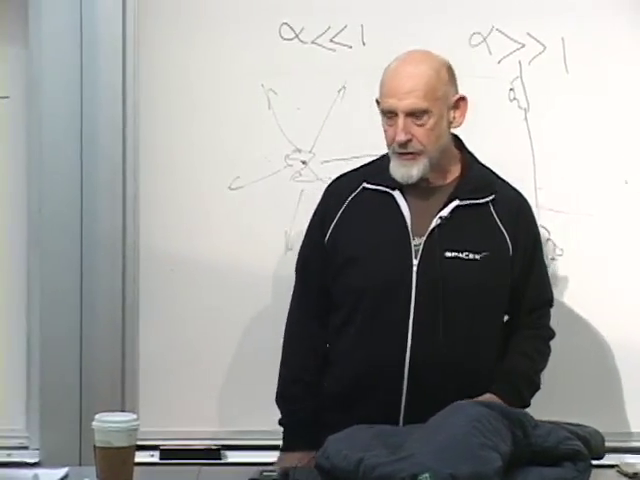
\includegraphics[width=0.72\textwidth]{lecture_01_figure_02.png}
\lectureframe{00:38:22.500}

\vspace{1em}

\begin{tikzpicture}[scale=0.95]
\draw (-5.3,-2.4) rectangle (-1.0,2.1);
\draw (0.3,-2.4) rectangle (4.6,2.1);

\node at (-3.15,2.55) {$\alpha \ll 1$};
\node at (2.45,2.55) {$\alpha \gg 1$};

\draw[line width=0.9pt] (-3.15,-0.15) circle (0.22);
\draw[->,line width=0.8pt] (-3.15,0.07) -- (-3.15,1.35);
\draw[->,line width=0.8pt] (-2.98,-0.01) -- (-1.95,1.00);
\draw[->,line width=0.8pt] (-3.32,-0.01) -- (-4.35,1.00);
\draw[->,line width=0.8pt] (-2.95,-0.23) -- (-1.80,-0.95);
\draw[->,line width=0.8pt] (-3.35,-0.23) -- (-4.50,-0.95);

\draw[line width=1.0pt] (2.15,-1.8) .. controls (1.95,-0.6) and (1.95,0.8) .. (2.15,1.55);
\draw[line width=1.0pt] (2.75,-1.8) .. controls (2.95,-0.6) and (2.95,0.8) .. (2.75,1.55);
\draw[line width=0.8pt] (2.15,-0.85) -- (2.75,-0.85);
\draw[line width=0.8pt] (2.45,1.55) -- (2.45,1.95);
\end{tikzpicture}\caption{Der Vergleich zwischen schwacher--starker Kopplung in der QED während der Diskussion über die Wechselwirkungsenergie. Die Abbildung stellt die beiden Regime einander gegenüber, die Susskind hier behandelt: eine dünne Wolke bei schwacher Kopplung und eine anwachsende Wolke bei starker Kopplung.}\end{figure}

Diese Abbildung gehört hierher, obwohl der Vergleich zwischen schwacher--starker Kopplung schon früher eingeführt wurde, weil Susskind den Gegensatz in der Vorlesung an dieser späteren, durch eine Frage angestoßenen Stelle bei der Diskussion der Wechselwirkungsenergie und der anwachsenden Struktur erneut zeichnet.

\section{Theorien mit geradzahligen Branen und die Entstehung einer zusätzlichen Dimension}

Bis hierher hat die Vorlesung einen deutlichen Austausch beschrieben: Fermion gegen Boson, Elektron gegen Monopol, F-String gegen D-String. Der nächste Schritt ist überraschender. Susskind wechselt zu einer anderen Variante der Stringtheorie, in der es geradzahlige statt ungeradzahlige D-Branen gibt. Dieser Unterschied ist wichtig, denn in dieser Theorie gibt es keinen D-String, der mit dem F-String ausgetauscht werden könnte. Es gibt D0-Branen, D2-Branen, D4-Branen und so weiter.

Der Grenzfall starker Kopplung kann daher nicht einfach darin bestehen, einen String durch einen anderen zu ersetzen. Laut Vorlesung geschieht etwas Seltsameres: Eine zusätzliche Raumdimension wird manifest. Susskind formuliert dies zunächst bewusst dramatisch --- ``eine neue Dimension wird sichtbar'' --- und präzisiert es unmittelbar darauf: Eine sehr kleine kompakte Richtung dehnt sich so weit aus, dass sie nicht länger vernachlässigt werden kann.

Auch die Zählung gehört zum Argument, daher hält er kurz inne:
\begin{equation}
\begin{aligned}
10\text{-dimensional string theory} &= 9\text{ space}+1\text{ time},\\
11\text{-dimensional theory} &= 10\text{ space}+1\text{ time}.
\end{aligned}
\end{equation}
Die Aussage der Vorlesung ist, dass die Theorie mit geradzahligen Branen im Grenzfall starker Kopplung effektiv elfdimensional ist.

\editorialnote{Die Theorie mit geradzahligen Branen ist die Stringtheorie vom Typ IIA; ihre Vervollständigung bei starker Kopplung ist die M-Theorie. In üblichen Einheiten skalieren der Radius des entstehenden Kreises und die elfdimensionale Planck-Länge wie folgt: \(R_{11}=g_s\ell_s\) und \(\ell_{11}=g_s^{1/3}\ell_s\). Diese Bezeichnungen und Formeln machen die moderne Zuordnung hinter der geometrischen Darstellung der Vorlesung ausdrücklich.}

\subsection{Das Erdnussbutter-Sandwich}

Um sich die kompakte Richtung vorzustellen, verwendet Susskind das Modell des ``Erdnussbutter-Sandwiches'': zwei unendlich dünne Brotscheiben mit realem Raum dazwischen. Die besondere Regel lautet, dass man auf der einen Seite hinausgeht und auf der anderen wieder hereinkommt. In einer üblichen Notation, die die Vorlesung bildlich statt formal beschreibt, kann man schreiben:
\begin{equation}
y \sim y + 2\pi R.
\end{equation}
Ist \(R\) sehr klein, beschreiben Beobachter, die im Sandwich leben, ihre Welt effektiv als niedrigdimensional. Die entscheidende Änderung bei starker Kopplung lautet dann:
\begin{equation}
g\uparrow
\qquad \Longrightarrow \qquad
R_{\mathrm{compact}}\uparrow.
\end{equation}
Wenn Susskind sagt, eine neue Raumdimension trete auf, meint er damit nicht, dass Raum aus dem Nichts entsteht. Vielmehr dehnt sich eine zuvor winzige kompakte Richtung aus und wird in der effektiven Theorie sichtbar.

\begin{figure}[htbp]\centering
\resizebox{\linewidth}{!}{%
\begin{tikzpicture}[scale=0.95]
\draw[line width=0.9pt] (-5,1.7) -- (5,1.7);
\draw[line width=0.9pt] (-5,-1.7) -- (5,-1.7);

\node[left] at (-5,1.7) {ceiling};
\node[left] at (-5,-1.7) {floor};

\draw[->,line width=0.8pt] (5.2,1.45) -- (5.2,-1.45);
\draw[->,line width=0.8pt] (5.5,-1.45) -- (5.5,1.45);
\node[right] at (5.55,0) {periodic};

\draw[line width=1.0pt] (-2.6,0.45) -- (2.2,0.45);
\draw[line width=1.0pt] (-2.6,-0.05) -- (2.2,-0.05);
\draw[line width=1.0pt] (-2.6,0.45) -- (-2.6,-0.05);
\draw[line width=1.0pt] (2.2,0.45) -- (2.2,-0.05);
\node at (-0.2,0.9) {floating D2-brane};

\draw[line width=1.0pt] (3.15,-1.7) -- (3.8,-1.7);
\draw[line width=1.0pt] (3.15,1.7) -- (3.8,1.7);
\draw[line width=1.0pt] (3.15,-1.7) -- (3.15,1.7);
\draw[line width=1.0pt] (3.8,-1.7) -- (3.8,1.7);
\node[right] at (3.95,0) {D2 ribbon};

\fill (-3.8,0) circle (0.07);
\node[below] at (-3.8,-0.05) {D0};
\end{tikzpicture}}%
\caption{Die Kompaktifizierung als Sandwich. Die obere und untere Begrenzung werden periodisch miteinander identifiziert. Eine D2-Brane schwebt dazwischen wie ein Teppich, während sich eine andere vom Boden bis zur Decke erstreckt und bei kleiner kompakter Richtung wie ein String aussieht.}\end{figure}

\subsection{Was wird aus den D0- und D2-Branen?}

Nun fragt die Vorlesung, was mit den D0-Branen und den Strings geschieht. Die Antwort fällt unterschiedlich aus. Mit wachsendem \(g\) werden die D0-Branen immer leichter; in der höherdimensionalen Deutung gehören sie zum Turm der Teilchen, die Impuls in der neu sichtbaren Richtung tragen. So wird ein schweres, kompliziertes Objekt in der Beschreibung bei schwacher Kopplung zu einer gewöhnlichen leichten Anregung in der Beschreibung bei starker Kopplung.

Die Massenbeziehung zeigt die Identifikation:
\begin{equation}
M_{D0}(n)=\frac{n}{g_s\ell_s}
=\frac{n}{R_{11}}
=M_{\mathrm{KK}}(n).
\end{equation}
\editorialnote{Susskind nennt die D0-Branen ``die Gravitonen'' der elfdimensionalen Theorie. Genauer gesagt sind ihre gebundenen Zustände die Kaluza--Klein-Impulsmoden des elfdimensionalen Supergravitationsmultipletts, dessen masseloser Sektor das Graviton enthält. Diese Unterscheidung erhält die physikalische Identifikation der Vorlesung, ohne ein einzelnes Teilchen zu behaupten.}

Die D2-Branen erklären, was aus den Strings wird. Die Vorlesung hebt zwei Konfigurationen hervor:
\begin{enumerate}
\item Eine D2-Brane schwebt wie ein Teppich in der Erdnussbutter zwischen Boden und Decke.
\item Eine D2-Brane erstreckt sich wie ein Band vom Boden bis zur Decke entlang der sichtbaren Richtung.
\end{enumerate}
Ist das Sandwich dünn, erscheint das Band effektiv eindimensional. Es ist das Objekt, das Beobachter bei niedrigen Energien als String bezeichnen. Öffnet sich die kompakte Richtung, wird dasselbe Objekt eindeutig membranartig. Da es nun auch in vertikaler Richtung mehr Ausdehnung besitzt, wird es schwer und verliert seinen stringartigen Charakter.

\paragraph{Die Logik des Übergangs.}
\begin{enumerate}
\item Man beginne mit einer sehr kleinen kompakten Dimension, sodass sich das Band von Boden bis Decke effektiv wie eine Saite verhält.
\item Erhöht man \(g\), so dehnt sich die kompakte Dimension aus.
\item Die D0-Branen werden leicht und als Kaluza--Klein-Impulszustände in der höherdimensionalen Theorie neu interpretiert.
\item Das saitenartige D2-Band wird zu einer sichtbar ausgedehnten Membran und wird schwer.
\end{enumerate}
Hier liegt der Übergang der Vorlesung von der Dualität zur emergenten Geometrie. Starke Kopplung tauscht nicht bloß ein Objekt gegen ein anderes aus; sie verändert, welche Geometrie die zweckmäßigste Beschreibung ist.

Susskind hält inne und betont, wie seltsam das klingt. Das Geflecht vorgeschlagener Identifikationen erforderte schwierige mathematische Konsistenzbeziehungen. Einige davon erschienen Physikern zunächst als Vermutungen und wurden später von Mathematikern bewiesen. Er behauptet nicht, dass jedes realistische Stringvakuum verstanden sei, sondern dass das Dualitätsgeflecht selbst ungewöhnlich strengen Prüfungen standgehalten hat.

Wenn die Kopplung in diesem idealisierten Szenario von Ort zu Ort variiert, kann sich auch die zweckmäßigste Geometrie mit ihr ändern. Eine Region kann nahezu zehn-dimensional erscheinen, mit leichten Strings und schweren D0-Branen; eine andere kann sich zur elfdimensionalen Beschreibung öffnen, mit schweren gewickelten Membranen und leichten Kaluza--Klein-Moden. Der lokale Wechsel der Beschreibung ist Teil desselben Dualitätsgeflechts.

Im Transkript wird der Name dieser Beziehungen kurz als ``Ungleichungen'' wiedergegeben. Gemeint ist im Zusammenhang jedoch \emph{Dualitäten}: Beziehungen zwischen den entgegengesetzten Enden des Parameterraums. Die Korrektur ist wichtig, denn die Schlussfolgerung der Vorlesung lautet gerade, dass keine eindeutige Liste fundamentaler Bestandteile bekannt ist. Strings, Branen, Teilchen und höherdimensionale Geometrie können ineinander übergehen; entweder ist kein Element des Geflechts absolut fundamental, oder eine tiefere Ordnung ist noch unbekannt.

\section{D3-Branen, gewickelte Membranen und ein geometrisches Bild der Dualität}

Nach der Pause beschreibt Susskind das Thema ausdrücklich als ein ``riesiges Geflecht'' miteinander verbundener Theorien und Ideen. Die folgenden Beispiele sind keine neuen, isolierten Effekte, sondern Verbindungen, die die zuvor behandelten Aspekte miteinander verknüpfen.

\subsection{Eine D3-Branen-Weltvolumen}

Die erste Verbindung beruht auf einer D3-Brane. Eine D3-Brane hat drei räumliche Dimensionen, und ein auf sie beschränkter Beobachter kann sie leicht für gewöhnlichen Raum halten. Die Brane kann sich krümmen und fluktuieren, während Strings, die auf ihr enden, sich verbinden, aufspalten und streuen können. Für einen Beobachter, der nur die Richtungen entlang der Brane sieht, erscheint jeder Endpunkt als Teilchen und die Wechselwirkungen zwischen den Endpunkten wie eine gewöhnliche Quantenfeldtheorie.

\begin{figure}[htbp]
\centering
\resizebox{\linewidth}{!}{%
\begin{tikzpicture}[scale=1.0]
\draw[fill=gray!15] (-4,-0.35) rectangle (4,0.35);
\node at (0,-0.75) {D3-brane};

\draw[line width=0.9pt] (-1.5,2.1) -- (-1.5,0.35);
\fill (-1.5,0.35) circle (0.07);
\node[left] at (-1.72,1.25) {F-string};
\node[below left] at (-1.5,0.32) {electric charge};

\draw[line width=1.5pt] (1.7,2.1) -- (1.7,0.35);
\fill (1.7,0.35) circle (0.09);
\node[right] at (1.95,1.25) {D-string};
\node[below right] at (1.7,0.32) {magnetic monopole};
\end{tikzpicture}
}%
\caption{Deutung über das Weltvolumen der D3-Brane. Der Endpunkt eines F-Strings erscheint als elektrische Ladung; der Endpunkt eines D-Strings als magnetischer Monopol.}
\end{figure}

Dies ist eine der überzeugendsten Identifikationen der Vorlesung. Für einen Beobachter auf dem Weltvolumen erscheint ein auf der D3-Brane endender F-String als elektrische Ladung. Ein auf derselben Brane endender D-String erscheint als magnetischer Monopol. Anders gesagt: Die Dualität zwischen F-Strings und D-Strings wird auf dem Weltvolumen der D3-Brane zur elektrisch--magnetischen Dualität der gewöhnlichen Feldtheorie. Was zuvor eine Analogie war, ist nun eine explizite Zuordnung.

\editorialnote{Für einen Stapel von D3-Branen ist die niederenergetische Beschreibung auf dem Weltvolumen eine vierdimensionale \(\mathcal N=4\) supersymmetrische Yang--Mills-Theorie. Ihre elektrisch--magnetische Dualität ist die feldtheoretische Realisierung der S-Dualität der Typ-IIB-Theorie; eine einzelne Brane liefert den in der Vorlesung bildlich dargestellten abelschen Grenzfall.}

\subsection{Zwei kompakte Dimensionen und asymmetrische Wicklung}

Anschließend kehrt Susskind zur höherdimensionalen Geometrie zurück und kompaktifiziert nicht eine, sondern zwei kleine Dimensionen. Da sich elf Dimensionen nicht an eine Tafel zeichnen lassen, fasst er die sieben großen, in der Skizze nicht verwendeten Dimensionen zu einer sichtbaren horizontalen Richtung zusammen und zeichnet die beiden kompakten Dimensionen ausdrücklich ein. Er besteht auf einer asymmetrischen Darstellung der Kompaktifizierung, denn eine kompakte Richtung muss kürzer sein als die andere, wenn die effektiven Strings unterschiedliche Spannungen haben sollen.

\begin{figure}[htbp]
\centering
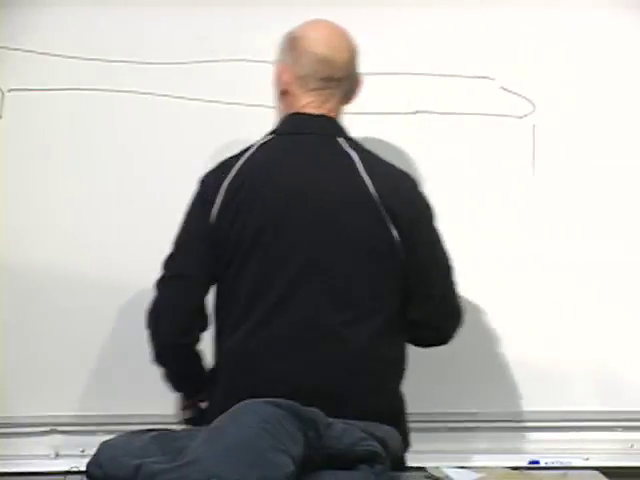
\includegraphics[width=0.78\textwidth]{lecture_01_figure_03.png}
\lectureframe{01:10:25.000}
\caption{Der fertige Tafelstand mit den beiden gewickelten Membranen. Die kurzen und langen kompakten Zyklen ergeben die rechts gezeichneten F- und D-stringartigen Bänder.}
\end{figure}

Eine Membran kann um eine der beiden kompakten Richtungen gewickelt sein und aus Sicht der nichtkompakten Richtungen wie ein String aussehen. Sind \(R_1\) und \(R_2\) die Radien der beiden Kreise, so lauten die effektiven Spannungen
\begin{equation}
\begin{aligned}
T_{(1)}&=2\pi R_1 T_{\mathrm{M2}},\\
T_{(2)}&=2\pi R_2 T_{\mathrm{M2}},\\
\frac{T_{(1)}}{T_{(2)}}&=\frac{R_1}{R_2}.
\end{aligned}
\end{equation}
Unterschiedliche Kreisgrößen führen also zu unterschiedlichen Stringspannungen. Identifiziert man die Wicklung um den kürzeren Kreis mit dem leichten F-String und die um den längeren mit dem schweren D-String, kann man schematisch schreiben:
\begin{equation}
g_s\sim \frac{R_{\mathrm{short}}}{R_{\mathrm{long}}},
\qquad
\frac{T_{\mathrm{D1}}}{T_{\mathrm{F1}}}\sim \frac{1}{g_s}.
\end{equation}

\begin{classroomqa}
\audiencequestion{Lässt sich die Kopplung in diesem Bild als Verhältnis der beiden kompakten Dimensionen verstehen? \lecturetimestamp{01:10:13}}
\lecturerresponse{Ja. Der Parameter für schwache--starke Kopplung wird geometrisch als Seitenverhältnis dargestellt. Wird eine Richtung verkürzt, ergibt sich eine kleine Kopplung; beim Vertauschen der beiden Richtungen werden die leichten und schweren Strings vertauscht.}
\end{classroomqa}

\editorialnote{In der Vorlesung wird dieses Verhältnis vorübergehend mit \(\alpha\) bezeichnet, wobei dasselbe Symbol wie zuvor für die Feinstrukturkonstante der QED verwendet wird. Hier schreiben wir \(g_s\), um die beiden Bedeutungen auseinanderzuhalten. In der vollständigen M-Theorie-Konstruktion ist die Kopplung der Typ-IIB-Theorie in der komplexen Struktur des kompakten Zweitorus kodiert; welcher Ausdruck genau im Zähler steht, hängt davon ab, wie seine Zyklen bezeichnet werden.}

Das Bild der gewickelten Membran lässt sich ohne die perspektivische Verzerrung der Tafelzeichnung so zusammenfassen:

\begin{figure}[htbp]
\centering
\begin{tikzpicture}[scale=1.0]
\draw[line width=0.9pt] (0,0) rectangle (5.2,2.2);
\node[below] at (2.6,-0.2) {\(R_1\)};
\node[right] at (5.4,1.1) {\(R_2\)};

\draw[->,line width=0.7pt] (5.45,1.9) -- (5.45,0.3);
\draw[->,line width=0.7pt] (5.7,0.3) -- (5.7,1.9);
\draw[->,line width=0.7pt] (0.4,-0.35) -- (4.8,-0.35);
\draw[->,line width=0.7pt] (4.8,-0.6) -- (0.4,-0.6);

\draw[line width=1.0pt] (1.1,0) -- (1.6,0) -- (1.6,2.2) -- (1.1,2.2) -- cycle;
\node at (1.35,2.55) {light};

\draw[line width=1.0pt] (0,1.45) -- (5.2,1.45);
\draw[line width=1.0pt] (0,1.00) -- (5.2,1.00);
\node at (4.55,1.95) {heavy};

\node at (1.35,-0.95) {F-string};
\node at (4.55,0.55) {D-string};
\end{tikzpicture}
\caption{Zwei gewickelte Membrankonfigurationen erscheinen aus Sicht der nichtkompakten Richtungen beide als Strings. Unterschiedliche kompakte Skalen sorgen jedoch dafür, dass einer der effektiven Strings leichter ist als der andere.}
\end{figure}

Dies ist die geometrische Version der zuvor erläuterten Dualität. Drückt man eine Richtung zusammen und dehnt die andere, wird das eine gewickelte Objekt schwerer und das andere leichter; so können F-String und D-String ihre Rollen tauschen.

\begin{classroomqa}
\audiencequestion{Sind die kompakten Richtungen zyklisch, sind die gewickelten Objekte dann unendlich breit? \lecturetimestamp{01:10:41}}
\lecturerresponse{Nein. Ein kompakter Kreis hat einen endlichen Umfang, obwohl man ihn wiederholt durchlaufen kann, ohne je einen Rand zu erreichen. Ober- und Unterkante der aufgeschnittenen Zeichnung stellen denselben Punkt dar, so wie die Endpunkte eines Intervalls denselben Punkt auf einem Kreis darstellen können.}
\end{classroomqa}

\begin{figure}[htbp]
\centering
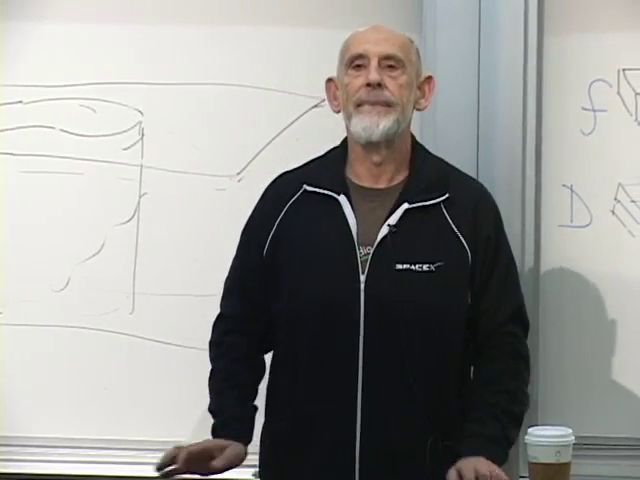
\includegraphics[width=0.78\textwidth]{lecture_01_figure_04.png}
\lectureframe{01:12:25.000}

\vspace{1em}

\begin{tikzpicture}[scale=0.95]
\draw[line width=0.9pt,->] (-3.7,0) arc[start angle=180,end angle=535,radius=0.95];
\node at (-2.75,0) {compact circle};
\draw[line width=0.9pt] (0.0,0) -- (4.8,0);
\fill (0.0,0) circle (0.06);
\fill (4.8,0) circle (0.06);
\draw[<->] (0.0,-0.45) -- (4.8,-0.45);
\node at (2.4,-0.75) {cut-open interval of length \(2\pi R\)};
\node[above] at (0.0,0.1) {same point};
\node[above] at (4.8,0.1) {same point};
\end{tikzpicture}
\caption{Ein kompakter Kreis und seine aufgeschnittene Darstellung an der Tafel. Überschreitet man den einen Endpunkt, gelangt man am anderen wieder hinein; bewegt man sich zugleich in einer nichtkompakten Richtung um den Kreis, beschreibt man dagegen eine Schraubenlinie.}
\end{figure}

\begin{classroomqa}
\audiencequestion{Warum ist der kompakte Weg ein Kreis und keine Schraubenlinie? \lecturetimestamp{01:12:23}}
\lecturerresponse{An jedem festen Punkt in der nichtkompakten Richtung ist die kompakte Richtung ein Kreis. Eine Schraubenlinie entsteht nur, wenn man sich in der nichtkompakten Richtung weiterbewegt und zugleich den Kreis umläuft. Das an der Tafel gezeichnete Intervall ist einfach ein aufgeschnittener Kreis, dessen beiden Endpunkte miteinander identifiziert werden.}
\end{classroomqa}

\begin{classroomqa}
\audiencequestion{Erklärt diese Geometrie selbst, wie eine D-Brane bei genauer Untersuchung wie eine Ansammlung von F-Strings aussehen kann? \lecturetimestamp{01:12:49}}
\lecturerresponse{Der Zusammenhang ist vorhanden, aber in diesem einfachen Bild nicht unmittelbar ersichtlich; um ihn zu erkennen, braucht es weitergehende geometrische Mittel. Die Skizze soll die Dualität ordnen, nicht jede mikroskopische Beschreibung der Bestandteile herleiten.}
\end{classroomqa}

\begin{classroomqa}
\audiencequestion{Können sich die langen und kurzen kompakten Richtungen beim Durchlaufen des Raums oder im Lauf der Zeit vertauschen? \lecturetimestamp{01:13:35}}
\lecturerresponse{Im idealisierten Modell ist beides möglich. Wird ein Zyklus gestaucht und der andere gedehnt, vertauscht sich, welcher gewickelte String leicht ist. Das ist ein weiterer Grund dafür, dass ``fundamentaler String'' nur eine Bezeichnung ist: Die zweckmäßigste Beschreibung kann sich von einer Region zur anderen oder mit der Zeit ändern.}
\end{classroomqa}

\section{Idealisierung, besonders symmetrische Punkte und die Landschaft}

Im letzten Teil der Vorlesung tritt Susskind von den eleganten Dualitätsbeispielen zurück und fragt, was sie uns über die reale Welt sagen und was nicht.

Zunächst warnt Susskind, dass die präzise kontrollierbaren Dualitäten Eigenschaften stark idealisierter supersymmetrischer Theorien sind, in denen Bosonen und Fermionen exakt übereinstimmende Massen haben. Als Analogie nennt er Kreisbahnen in der Newtonschen Mechanik: Man untersucht sie zuerst, weil sie symmetrisch und mathematisch handhabbar sind, nicht weil sich die tatsächliche Planetenbewegung auf perfekte Kreise beschränkt. Genauso lassen sich supersymmetrische Stringtheorien leichter analysieren, weil sie symmetrischer sind als die Natur zu sein scheint.

Die Idealisierung ist dennoch aufschlussreich. Eine perfekte Kreisbahn ist kein realistisches Planetensystem, zeigt aber Eigenschaften, die auch bei weniger symmetrischen Bahnen erhalten bleiben. Ebenso zeigen die supersymmetrischen Beispiele konsistente Möglichkeiten, Quantenmechanik, Gravitation und mikroskopische Struktur miteinander zu vereinbaren. Susskind formuliert bewusst zugespitzt: Die handhabbaren Stringtheorien sind buchstäblich nicht die Theorie unserer Welt; ihr Wert liegt darin, dass sie Phänomene offenbaren, die wahrscheinlich auch in weniger symmetrischen und weniger handhabbaren Situationen wieder auftreten.

\subsection{Ein Baukasten mit vielen möglichen Ergebnissen}

D-Branen sind nur ein Teil des verfügbaren Baukastens. Die Vorlesung nennt auch Flüsse, Orbifolds und Orientifolds. Zunächst wählt man eine kompakte Geometrie und dann, welche Branen und Flüsse ihre Zyklen besetzen. Selbst beim einfachen Sandwich ändert sich die niederdimensionale Physik, wenn man eine schwebende D2-Brane, zwei oder drei einfügt. Fügt man solche Bestandteile hinzu oder entfernt sie, ändern sich die effektiven Teilchen, Wechselwirkungen und Parameter.

Angenommen, ein sechsdimensionaler kompakter Raum habe in der schematischen Zählung der Vorlesung etwa \(500\) Zyklen, und für jeden Zyklus gebe es ungefähr \(10\) Möglichkeiten, gewickelte Branen, Flüsse oder verwandte Strukturen zu wählen. Dann wächst die Zahl der Konstruktionen wie
\begin{equation}
N_{\mathrm{vacua}} \sim 10^{500}.
\end{equation}
Die Zähllogik der Vorlesung ist einfach:
\begin{equation}
10 \times 10 \times \cdots \times 10 = 10^{500}
\end{equation}
mit \(500\) Faktoren. Die Analogie mit der DNA verdeutlicht denselben Punkt auf vertrautere Weise:
\begin{equation}
N_{\mathrm{DNA}}(500)=4^{500}.
\end{equation}
Während des DNA-Vergleichs fragt ein Zuhörer nach und vergewissert sich, dass es entlang eines Strangs vier Alternativen gibt: A, C, G und T. Die Korrektur verstärkt das Argument, statt es zu verändern. Eine kurze Liste lokaler Möglichkeiten, viele Male wiederholt, ergibt eine riesige Zahl globaler Anordnungen. Der genaue Exponent ist nicht entscheidend, und Susskind bezeichnet \(10^{500}\) als alte Unterschätzung; entscheidend ist die kombinatorische Vervielfachung.

Damit kehrt sich die reduktionistische Erwartung vom Anfang der Vorlesung endgültig um. Eine komplizierte Teilchenphysik muss nicht aus komplizierten mikroskopischen Regeln hervorgehen. Sie kann entstehen, weil unser Vakuum eine komplizierte Anordnung vieler einfacher Bestandteile ist, so wie ein komplexer Organismus durch eine Sequenz kodiert sein kann, die aus vier Basen aufgebaut ist.

\begin{classroomqa}
\audiencequestion{Würde vollständige Kenntnis nach der Identifizierung dualitätsverwandter äquivalenter Beschreibungen nur ein oder wenige dieser möglichen Vakua als Beschreibungen unserer Welt auswählen? \lecturetimestamp{01:26:11}}
\lecturerresponse{Vermutlich würde sie eine eingeschränkte Menge auswählen, doch viele verschiedene Vakua könnten bei zugänglichen Energien äußerst ähnlich aussehen. Die zitierte Anzahl möglicher Vakua soll auch nach der Identifizierung dualer Beschreibungen groß bleiben, und irrelevante Details bei hohen Energien können wie ``„Junk-DNA“''} wirken.\end{classroomqa}

\subsection{Symmetrische Punkte und generische Komplexität}

In der Landschaft gibt es besonders symmetrische Punkte. Im geometrischen Bild macht eine Konfiguration mit gleichen Seitenverhältnissen,
\begin{equation}
R_1=R_2,
\end{equation}
die beiden gewickelten Beschreibungen gleichermaßen einfach. In der Analogie mit elektrisch--magnetischer Dualität wird dies schematisch dargestellt durch
\begin{equation}
m_{\mathrm{monopole}}=m_e.
\end{equation}

\begin{figure}[htbp]
\centering
\begin{tikzpicture}[scale=0.95]
\draw[line width=0.9pt] (-4.5,-1.0) rectangle (-2.5,1.0);
\draw[<->] (-4.5,-1.35) -- (-2.5,-1.35);
\draw[<->] (-2.15,-1.0) -- (-2.15,1.0);
\node at (-3.5,1.45) {symmetric point};
\node at (-3.5,-1.75) {$R_1=R_2$};

\draw[line width=0.9pt] (0.0,-0.55) rectangle (4.8,0.55);
\draw[<->] (0.0,-0.9) -- (4.8,-0.9);
\draw[<->] (5.15,-0.55) -- (5.15,0.55);
\node at (2.4,1.45) {lopsided point};
\node at (2.4,-1.3) {$R_1\ne R_2$};
\end{tikzpicture}
\caption{Eine Kompaktifizierung mit gleichen Seitenverhältnissen behandelt die beiden gewickelten Strings symmetrisch; bei einer stark verzerrten Kompaktifizierung ist eine der Beschreibungen deutlich leichter als die andere.}
\end{figure}

\begin{classroomqa}
\audiencequestion{Gibt es in der Landschaft Vakua, bei denen die Konstruktion viel einfacher wird, weil die Beschreibungen durch F- und D-Strings zusammenfallen? \lecturetimestamp{01:27:21}}
\lecturerresponse{Ja, es gibt besonders symmetrische Punkte. Unsere Welt scheint sich nicht an einem solchen Punkt zu befinden: Das vertraute elektrische Teilchen und ein magnetischer Monopol haben nicht dieselbe Masse. Warum die Natur einen verzerrten Punkt einnimmt, ist unbekannt.}
\end{classroomqa}

\editorialnote{Die Gleichheit der Elektronen--- und Monopolmasse ist ein schematisches Merkmal eines geeignet geschützten selbstdualen Modells, keine Vorhersage der gewöhnlichen, nichtsupersymmetrischen QED. Sie bringt die Idee des symmetrischen Punkts aus der Vorlesung zum Ausdruck und ist keine Behauptung über das beobachtete Elektron.}

Anschließend erinnert Susskind an eine Analogie aus der Kommunikationstheorie. Zufällige Codes können außerordentlich gut sein, während die am einfachsten zu beschreibenden und zu dekodierenden Codes zusätzliche mathematische Struktur haben und sich historisch weniger gut bewährten. Später fand die Codierungstheorie hochwirksame strukturierte Konstruktionen, doch die Analogie bleibt bestehen: Alles, was sich knapp benennen oder beschreiben lässt, liegt in einer besonders speziellen, niedrigkomplexen Ecke des gesamten Möglichkeitsraums. Ebenso können die am leichtesten berechenbaren Stringvakua untypisch einfach sein.

Daher könnten sich die passenden Fragen ändern. Statt die genaue Kompaktifizierung bis ins mikroskopische Detail zu verlangen, kann man fragen, welche Merkmale in einem breiten Ensemble häufig oder generisch sind. Susskind stellt dies als Forschungsproblem dar, nicht als gesicherte Schlussfolgerung, und lehnt ideologische Argumente anstelle von Berechnungen ab.

\subsection{Kosmologische Fragen}

\begin{classroomqa}
\audiencequestion{Unterscheidet sich eine kompakte Richtung mit enormem Umfang bei Beobachtungen von einer unendlichen Richtung, und wissen wir, dass unsere drei großen Raumdimensionen unendlich sind? \lecturetimestamp{01:30:03}}
\lecturerresponse{Wir wissen nicht, ob sie unendlich sind. Eine geschlossene Dreisphäre kann sich ausdehnen und dabei kompakt bleiben. Messungen der nahezu flachen Geometrie liefern lediglich eine untere Schranke für den Krümmungsradius, so wie eine Vermessung eines nahezu ebenen Feldes die Größe der Erde eingrenzen kann, ohne zu beweisen, dass ihre Oberfläche unendlich ist. Erst eine nachgewiesene Krümmung oder globale Identifikation würde die endliche Skala bestimmen.}
\end{classroomqa}

\begin{classroomqa}
\audiencequestion{Wenn die Kopplung im idealisierten Modell räumlich variieren kann, wie könnte eine solche Variation in der realen Welt auftreten? \lecturetimestamp{01:32:43}}
\lecturerresponse{Nicht als die uneingeschränkte, glatte Variation im symmetrischen Beispiel. Die realistische Möglichkeit, die später behandelt wird, ist eine Variation durch diskrete Übergänge zwischen Regionen mit unterschiedlichen effektiven Gesetzen. Ob solche Sprünge auftreten, ist eine kosmologische Frage.}
\end{classroomqa}

\editorialnote{Diese Antwort ist als Vorausblick der Vorlesung auf Flussvakua und Übergänge zwischen Domänen zu verstehen, nicht als allgemeiner Satz, der jedes glatt variierende Skalarfeld ausschließt. Beobachtungen setzen Variationen dimensionsloser Kopplungen enge Grenzen; Stabilisierungsmechanismen bestimmen, ob in einem bestimmten Modell kontinuierliche Moduli verfügbar bleiben.}

Die Aufnahme enthält die letzte Frage aus dem Publikum nicht. Aus der erhaltenen Antwort geht hervor, dass das vorgeschlagene Phänomen bei bestimmten Arten von Schwarzen Löchern auftreten kann, nicht jedoch am Horizont eines gewöhnlichen Schwarzschild-Schwarzen-Lochs, dessen Horizont für einen frei fallenden Beobachter lokal ein gewöhnlicher Ort ist. Da sich die Frage nicht zuverlässig rekonstruieren lässt, wird dem Wortwechsel keine spezifischere Aussage zugeschrieben.

\section{Von Bausteinen zu einem Geflecht von Beschreibungen}

Die Hoffnung, dass tiefere Schichten der Physik einfacher sein müssen, hat sich als trügerisch erwiesen. Bei der \(1+1\)-dimensionalen Bosonisierung kann dieselbe Theorie entweder in Begriffen von Fermionen oder von Bosonen formuliert werden, wobei das Fermion als Kink wieder auftritt. In der Quantenelektrodynamik tauschen schwache und starke Kopplung die beschreibenden Rollen von Elektron und magnetischem Monopol aus. In der Stringtheorie wiederholen F-Strings und D-Strings dasselbe Muster. In der Theorie geradzahliger Branen geht die starke Kopplung noch weiter: Eine kompakte Richtung dehnt sich aus, D0-Branen werden zu Kaluza--Klein-Impulszuständen, und effektive Strings werden als gewickelte Membranen in einer höherdimensionalen Geometrie neu interpretiert. Die moderne Quantenfeldtheorie und Stringtheorie liefern daher keine einzigartige, ein für alle Mal feststehende Antwort auf die Frage ``Was sind die Bausteine und was die Häuser?'' Sie liefern ein Geflecht von Beschreibungen, deren jede in ihrem eigenen Bereich zweckmäßig ist, sowie eine riesige Landschaft möglicher Konstruktionen, deren generisches Ergebnis Komplexität statt Einfachheit ist.

\chapter{Geometrie, Information und das Flächengesetz für Schwarze Löcher}

\lectureoverview{Das angekündigte Ziel ist die Kosmologie, doch der kürzeste Weg dorthin beginnt mit einer Rückkehr zur speziellen Relativitätstheorie. Eine Metrik beschreibt die Geometrie der Raumzeit, und die Bedingung verschwindender Eigenzeit beschreibt, wie sich Licht bewegt. Wir übertragen diese eine Regel auf die Schwarzschild-Geometrie, unterscheiden den Horizont von der Singularität und fragen dann, was mit Information geschieht, wenn ein Schwarzes Loch ausstrahlt und verdampft. Die Antwort beginnt mit gewöhnlicher Entropie und endet bei Bekensteins Argument mit einem Bit: Ein Schwarzes Loch speichert Information in Einheiten der Horizontfläche, nicht des Volumens.}

Susskind verschiebt kurz eine angekündigte Bilanz der Erfolge und Misserfolge der Stringtheorie. Es sei spät, sagt er, und die inhaltliche Substanz sei nützlicher als eine Bilanz. Heute Abend geht es um die minimale Geometrie und Thermodynamik, die nötig sind, um das Informationsproblem Schwarzer Löcher zu formulieren.

\section{Eine Regel für Licht}

Die spezielle Relativitätstheorie behandelt Raum und Zeit als ein gemeinsames geometrisches Objekt. Für benachbarte Ereignisse mit dem Abstand \(dt,dx,dy,dz\) verwendet Susskind die Vorzeichenkonvention mit überwiegend positiven Vorzeichen und schreibt
\begin{equation}
d\tau^2=dt^2-\frac{1}{c^2}\left(dx^2+dy^2+dz^2\right).
\end{equation}
Die entgegengesetzten Vorzeichen der zeitlichen und räumlichen Anteile unterscheiden die Minkowski-Geometrie von der vierdimensionalen euklidischen Geometrie. Der Faktor \(1/c^2\) dient lediglich dem Ausgleich der Einheiten; wenn wir Zeit und Entfernung miteinander verträglich messen, können wir \(c=1\) setzen.

Für zeitartige Abstände gilt \(d\tau^2>0\), und \(d\tau\) ist die Eigenzeit, die eine Uhr entlang der Bahn aufzeichnet. Bei raumartigen Abständen gilt dagegen \(d\tau^2<0\). Der heute Abend benötigte Fall liegt genau dazwischen. Ein Lichtstrahl folgt einer \emph{lichtartigen} Bahn,
\begin{equation}
d\tau^2=0.
\end{equation}
Beschränken wir uns zunächst auf eine Bewegung entlang der \(x\)-Achse, so ergibt sich
\begin{align}
0&=dt^2-\frac{dx^2}{c^2},\\
c\,dt&=\pm dx,\\
\frac{dx}{dt}&=\pm c.
\end{align}
Die Vorzeichen beschreiben nach rechts und nach links laufende Strahlen. Der Zahlenwert, der \(c\) zugeordnet wird, ändert sich, wenn Zentimeter durch Meter oder Kilometer ersetzt werden; die invariante Aussage ist keine Zahl, sondern die Nullbedingung.

Die allgemeine Relativitätstheorie macht die Metrik komplizierter, nicht aber diese Regel. Mit den Koordinaten \(x^\mu\), \(\mu=0,1,2,3\) gilt
\begin{equation}
ds^2=g_{\mu\nu}(x)\,dx^\mu dx^\nu,
\end{equation}
wobei über wiederholte Indizes summiert wird und die Koeffizienten sich von Punkt zu Punkt ändern können. Um die lokal möglichen Richtungen des Lichts zu bestimmen, setzt man diese quadratische Form gleich null.

\section{Kugelkoordinaten und die Schwarzschild-Metrik}

Ein nichtrotierendes Schwarzes Loch ist kugelsymmetrisch, daher verdecken kartesische Koordinaten die nützliche Struktur. \(r\) bezeichne den radialen Abstand und \(\theta,\phi\) die Richtung auf einer Einheitskugel. Das Linienelement lautet
\begin{equation}
d\Omega^2=d\theta^2+\sin^2\theta\,d\phi^2.
\end{equation}
Auf einer Kugel mit Radius \(r\) tragen Winkelverschiebungen daher \(r^2d\Omega^2\) bei. Die flache Raumzeit lautet in Kugelkoordinaten
\begin{equation}
d\tau^2=dt^2-\left(dr^2+r^2d\Omega^2\right),
\qquad (c=1).
\end{equation}

Susskind leitet die Lösung für das Schwarze Loch nicht aus Einsteins Gleichungen her. Er schreibt sie hin und bittet uns, sie zu betrachten. Die Tafel macht den beabsichtigten Vergleich deutlich.

\begin{figure}[htbp]
\centering
\includegraphics[width=0.86\textwidth]{lecture_02_figure_02.png}
\caption{Flache Raumzeit in Kugelkoordinaten oberhalb der Schwarzschild-Verformung. Der gemeinsame Faktor \(1-2GM/(c^2r)=1-R_s/r\) und die radiale Skizze sind gleichzeitig zu sehen.}
\lectureframe{00:19:12.520}
\end{figure}

Für ein Schwarzes Loch der Masse \(M\) definieren wir den Schwarzschild-Radius
\begin{equation}
R_s=\frac{2GM}{c^2}.
\end{equation}
Das Linienelement außerhalb des Lochs lautet
\begin{equation}
d\tau^2=\left(1-\frac{R_s}{r}\right)dt^2
-\frac{dr^2/c^2}{1-R_s/r}
-\frac{r^2}{c^2}d\Omega^2.
\label{eq:schwarzschild-explicit-c}
\end{equation}
Äquivalent dazu gilt nach der Setzung \(c=1\)
\begin{equation}
ds^2=\left(1-\frac{2GM}{r}\right)dt^2
-\frac{dr^2}{1-2GM/r}-r^2d\Omega^2.
\label{eq:schwarzschild}
\end{equation}
In großer Entfernung gilt \(R_s/r\ll1\), und die flache Metrik in Kugelkoordinaten ergibt sich zurück. Diese asymptotische Überprüfung ist wichtiger, als die Formel auswendig zu lernen, obwohl Susskind Letzteres als Stoff für Cocktailpartys empfiehlt.

\editorialnote{Auf der Tafel wechseln sich \(d\tau^2\) und \(ds^2\) ab, und nicht jeder Faktor \(c\) wird durchgängig angegeben. Gleichung~\eqref{eq:schwarzschild-explicit-c} folgt der Zeitkoordinatenkonvention der Vorlesung, nach der \(t\) die Einheit einer Zeit hat. Die Standardform mit \(x^0=ct\) ist algebraisch äquivalent.}

\subsection{Der Horizont ist nicht die Singularität}

Bei zwei Radien wirken die Koordinaten verdächtig. Bei \(r=R_s=2GM\) in natürlichen Einheiten verschwindet der Koeffizient von \(dt^2\), während der von \(dr^2\) divergiert. Bei \(r=0\) wird die Krümmung selbst singulär. Das sind keine zwei Varianten desselben Ereignisses:
\begin{equation}
\begin{aligned}
r=R_s &:\quad \text{horizon},\\
r=0 &:\quad \text{curvature singularity}.
\end{aligned}
\end{equation}

Gezeitenkräfte machen den physikalischen Unterschied deutlich. Ein Gravitationsfeld ist über einen ausgedehnten Körper hinweg unterschiedlich: Die Füße können stärker als der Kopf angezogen werden, wodurch der Körper gedehnt und zugleich in Querrichtung zusammengedrückt wird. Am Horizont sind diese Gezeitenkräfte endlich; am Horizont eines hinreichend massereichen Schwarzen Lochs können sie sehr klein sein. Dort muss sich nichts lokal Katastrophales ereignen. Bei \(r=0\) divergieren die Gezeitenkräfte dagegen. Die alarmierenden Koeffizienten bei \(r=R_s\) weisen auf einen Mangel der Schwarzschild-Koordinaten hin; die Singularität bei \(r=0\) ist physikalisch.

\editorialnote{Dass die Krümmung bei \(r=R_s\) endlich ist, lässt sich am Kretschmann-Skalar \(R_{\mu\nu\rho\sigma}R^{\mu\nu\rho\sigma}=48G^2M^2/(c^4r^6)\) überprüfen, der am Horizont endlich ist und nur für \(r\to0\) divergiert. Diese Invariante kam in der Vorlesung nicht vor, präzisiert aber den dort erläuterten Unterschied bei den Gezeitenkräften.}

\section{Radiales Licht in Horizontnähe}

Kehren wir nun zu der einen Regel zurück. Ein radialer Strahl behält seine Winkelposition bei, also gilt \(d\Omega=0\), und für einen Lichtstrahl gilt \(ds^2=0\). In Einheiten mit \(c=1\) ergibt Gleichung~\eqref{eq:schwarzschild}
\begin{equation}
0=\left(1-\frac{2GM}{r}\right)dt^2
-\frac{dr^2}{1-2GM/r}.
\end{equation}
Multiplikation mit \(1-2GM/r\) und anschließendes Wurzelziehen liefern zwei Zweige,
\begin{align}
dr&=\pm\left(1-\frac{2GM}{r}\right)dt,\\
\frac{dr}{dt}&=\pm\left(1-\frac{2GM}{r}\right).
\label{eq:radial-null}
\end{align}
Das Pluszeichen steht für auslaufendes, das Minuszeichen für einlaufendes Licht. In großer Entfernung nähern sich ihre Koordinatengeschwindigkeiten \(\pm1\). Am Horizont gilt für beide \(\lvert dr/dt\rvert\to0\): In Schwarzschild-Koordinatenzeit scheint ein auslaufender Strahl dort stillzustehen, während ein einlaufender Strahl unendlich viel Koordinatenzeit bis zu seiner Ankunft benötigt.

\begin{figure}[htbp]
\centering
\includegraphics[width=0.82\textwidth]{lecture_02_figure_03.png}
\caption{Die vervollständigte Tafelzeichnung im \(t\)-\(r\)-Diagramm: Radiale Nullstrahlen verlaufen nahezu senkrecht, wenn sie sich dem gestrichelten Horizont nähern.}
\lectureframe{00:30:25.000}
\end{figure}

\begin{figure}[htbp]
\centering
\begin{tikzpicture}[x=1.0cm,y=0.9cm]
\draw[->] (0,0) -- (6.6,0) node[right] {$r$};
\draw[->] (0,0) -- (0,6.2) node[above] {$t$};
\draw[dashed,thick] (2.0,0) -- (2.0,5.9) node[above] {$r=R_s$};
\draw[thick,->] (2.08,.4) .. controls (2.10,2.2) and (2.55,3.8) .. (5.8,5.7);
\draw[thick,->] (5.8,.5) .. controls (3.2,2.0) and (2.15,4.2) .. (2.03,5.7);
\node[align=center] at (4.7,4.4) {outgoing};
\node[align=center] at (4.5,1.2) {ingoing};
\end{tikzpicture}
\caption{Eine bereinigte Fassung der Tafelzeichnung in Koordinatenzeit. Die scheinbare Verlangsamung betrifft \(t\) in Schwarzschild-Koordinaten, nicht ein lokales Versagen des Lichts, sich mit \(c\) zu bewegen.}
\end{figure}

Innerhalb des Horizonts sind die zukünftigen Lichtkegel so weit nach innen geneigt, dass beide zukunftsgerichteten radialen Zweige zu kleinerem \(r\) führen. Kein Signal, das von dort ausgeht, kann nach außen entkommen, und jeder zukunftsgerichtete kausale Weg erreicht die Singularität.

\begin{classroomqa}
\audiencequestion{Wenn die Lichtgeschwindigkeit invariant ist, was genau bedeutet dann die Aussage, dass sich Licht in Horizontnähe verlangsamt?\lecturetimestamp{00:31:44}}
\lecturerresponse{Die dargestellte Größe ist \(dr/dt\) in einem bestimmten Koordinatensystem. Schon die Angabe einer Geschwindigkeit als Zahl ändert sich, wenn Meter durch Zentimeter ersetzt werden; hier variieren die effektiven radialen und zeitlichen Maßstäbe mit dem Ort. Die universelle Aussage lautet, dass jeder Lichtstrahl einer Nullbahn folgt: \(ds^2=0\).}
\end{classroomqa}
\editorialnote{Ein frei fallender lokaler Beobachter misst für Licht im Vakuum \(c\); die verschwindende Schwarzschild-Koordinatengeschwindigkeit am Horizont ist keine lokal beobachtbare Größe.}

\begin{classroomqa}
\audiencequestion{Gilt dieselbe Aussage über die Nullgeschwindigkeit unabhängig vom materiellen Medium, durch das sich das Licht bewegt?\lecturetimestamp{00:33:24}}
\lecturerresponse{Nein. Die verfügbare Aufzeichnung enthält keine längere Erklärung dieser Antwort.}
\end{classroomqa}
\editorialnote{Die Aussage über die Nullgeschwindigkeit betrifft die Ausbreitung in der Vakuumraumzeit. Wechselwirkungen mit Materie können einem Wellenpaket eine geringere effektive Geschwindigkeit verleihen; das ist eine Eigenschaft des Mediums und keine Änderung der lokalen kausalen Geschwindigkeit \(c\).}

\begin{classroomqa}
\audiencequestion{Wie sieht ein einlaufender Lichtstrahl im selben \(t\)-\(r\)-Diagramm aus?\lecturetimestamp{00:33:32}}
\lecturerresponse{Er ist der umgekehrt erscheinende Zweig: Ausgehend von großem \(r\) biegt er zum Horizont hin ab und nähert sich diesem asymptotisch. Bis zur Ankunft vergeht eine unendliche Koordinatenzeit \(t\).}
\end{classroomqa}
\editorialnote{Ein einfallender Beobachter erreicht und durchquert den Horizont in endlicher Eigenzeit; nur die Schwarzschild-Koordinatenzeit \(t\) divergiert.}

\section{Warum die Verdampfung ein Problem aufwirft}

Der Horizont verdient eine viel eingehendere Untersuchung: wie er entsteht, was ein einfallender Beobachter sieht und ob sich dort lokal etwas Ungewöhnliches ereignet. Susskind vertagt diese Fragen und springt zur Quantenmechanik. Von außen betrachtet werden Materie und sämtliche unterscheidenden Informationen immer näher an den Horizont herangedrückt und unzugänglich. Das allein muss keine Information vernichten; sie könnte lediglich verborgen sein.

Hawkings Ergebnis macht das Problem akut. Ein klassisches Schwarzes Loch im Gleichgewicht wirkt wie das langweiligste denkbare Objekt: kugelförmig, dunkel und unfähig, eine Nachricht zu senden. Doch ``schwarz'' hat zwei Bedeutungen. Es kann heißen, dass nichts ausgestrahlt wird, oder dass thermische Schwarzkörperstrahlung ausgesandt wird. Ein quantenmechanisches Schwarzes Loch ist im zweiten Sinn schwarz. Es hat eine Temperatur, leuchtet und verliert Energie. Da
\begin{equation}
E=Mc^2,
\qquad
R_s=\frac{2GM}{c^2},
\end{equation}
verringert die Strahlung sowohl seine Masse als auch seinen Horizont-Radius. Was geschieht mit der Information, die am Horizont verblieben zu sein schien, wenn das Loch schließlich verdampft? Sie könnte vernichtet, in einem winzigen Überrest eingeschlossen oder in der auslaufenden Strahlung kodiert sein. Die Spannung zwischen diesen Möglichkeiten ist das Informationsproblem, und die Stringtheorie wird später helfen, seine Lösung genauer zu fassen.

Heute Abend wird keine Berechnung von Quantenfeldern in gekrümmter Raumzeit vorgenommen. Stattdessen folgt Susskind Bekensteins einfacherer Vorgehensweise: Zuerst verstehen wir Entropie als Information und berechnen dann, wie viel Information ein Schwarzes Loch verbergen kann.

\section{Information, die vorhanden, aber verborgen ist}

Stellen wir uns vor, eine Schachtel werde in Zellen unterteilt, die so klein sind, dass jede entweder belegt oder leer ist. Eine binäre Zeichenfolge---eine Antwort pro Zelle---unterscheidet die jeweilige Konfiguration von jeder anderen zulässigen Konfiguration. Für realistischere Materie muss man auch nach Teilchensorten und weiteren Freiheitsgraden fragen, aber das Prinzip bleibt gleich: Information wird durch die Mindestzahl an Ja--Nein-Fragen gemessen, die nötig ist, um den Zustand festzulegen.

\begin{classroomqa}
\audiencequestion{Beschreibt das nur ein statisches System?\lecturetimestamp{00:45:49}}
\lecturerresponse{Es ist eine Momentaufnahme zu einem bestimmten Zeitpunkt. Die Dynamik bildet diesen Zustand dann auf einen anderen ab.}
\end{classroomqa}

Das nächste Prinzip geht tiefer: Die Entwicklung eines abgeschlossenen Systems führt nicht zwei verschiedene mikroskopische Zustände zu einem einzigen zusammen. Unterscheiden sich zwei Konfigurationen jetzt, bleiben auch ihre entwickelten Konfigurationen prinzipiell unterscheidbar. Die klassische Hamiltonsche Entwicklung ist umkehrbar, die quantenmechanische Entwicklung unitär.\editorialnote{Dissipative effektive Gleichungen können Unterschiede nur deshalb auslöschen, weil unbeobachtete Freiheitsgrade der Umgebung weggelassen wurden; der vollständige Zustand des abgeschlossenen Systems bewahrt sie.}

Die Badewanne macht den Unterschied zwischen Verlust und Unzugänglichkeit anschaulich. Zwei Tropfenströme könnten zwei verschiedene Morsecode-Nachrichten kodieren. Nachdem sich das Wasser beruhigt hat, sehen beide Wannen gleich aus. Die sichtbaren Wellen sind verschwunden, doch eine vollständige mikroskopische Messung würde weiterhin unterschiedliche Molekülkonfigurationen ergeben. Die Nachricht hat sich auf Freiheitsgrade verteilt, die zu klein und zu zahlreich sind, um sie zu verfolgen.

Entropie ist diese verborgene Information. Gemessen an den makroskopischen Fragen, die wir stellen können---Temperatur, Gesamtenergie, Zusammensetzung, Wasserstand---, bleiben viele mikroskopische Unterschiede möglich, aber unzugänglich. In der Bit-Zählweise der Vorlesung gilt
\begin{equation}
S=\hbox{number of hidden bits}.
\end{equation}
Die genaue statistische Formel lautet \(S=k_B\ln\Omega\), doch für das Argument zu Schwarzen Löchern genügt die qualitative Definition.

\section{Temperatur als Preis für das Verbergen eines Bits}

Temperatur lässt sich leicht messen, aber überraschend indirekt definieren. Susskind wählt Entropie und Energie als Grundbegriffe. Angenommen, ein Computerbit wird auf einen Standardwert zurückgesetzt. Das physische Gerät bleibt bestehen, doch der Unterschied zwischen seinem früheren Null- und Einszustand verschwindet im Computer. Aus der vollständigen Welt kann er nicht verschwinden; er wird auf mikroskopische Freiheitsgrade der Umgebung übertragen, die sich dadurch geringfügig erwärmt. Das ist das Landauer-Prinzip.

Wenn eine Entropieeinheit einem Bit entspricht und die Temperatur in Energieeinheiten gemessen wird, schreibt die Vorlesung
\begin{align}
\Delta S&=1,\\
\Delta E&=T\,\Delta S,\\
dE&=T\,dS.
\label{eq:first-law}
\end{align}

\begin{figure}[htbp]
\centering
\includegraphics[width=0.84\textwidth]{lecture_02_figure_04.png}
\caption{Die informationstheoretische Thermodynamik auf der Tafel: \(S\) ist die Entropie, ein verborgenes Bit entspricht \(\Delta S=1\), und sein minimaler Energieaufwand wird mit \(\Delta E=T\Delta S\) angegeben.}
\lectureframe{00:58:40.000}
\end{figure}

\editorialnote{In konventionellen Einheiten beträgt der reversible Löschaufwand für ein binäres Bit \(k_BT\ln2\). Gleichung~\eqref{eq:first-law} verwendet \(k_B=1\) und behandelt die Entropieeinheit der Vorlesung als ein Bit, wobei der zugehörige Faktor \(\ln2\) unterdrückt wird. Diese Konventionen ändern nichts an der folgenden Skalierungsbetrachtung.}

Eine Schätzung aus dem Publikum beziffert den minimalen Temperaturanstieg beim Löschen von etwa \(100\) Gigabyte in einem Glas Wasser auf ungefähr \(10^{-15}\) Grad. Susskind lässt die genaue Zahl dahingestellt und übernimmt den wesentlichen Punkt: Bei Raumtemperatur trägt ein Bit eine außerordentlich kleine minimale Energie, und reale Computer dissipieren erheblich mehr, weil das Löschen nicht reversibel erfolgt.

\begin{classroomqa}
\audiencequestion{Ist das Festplattenbeispiel nur eine Analogie, oder ist die Erwärmung beim Löschen ein echtes Gesetz?\lecturetimestamp{01:00:02}}
\lecturerresponse{Es handelt sich um eine echte physikalische Einschränkung, die Landauer-Regel. Beim Zurücksetzen einer Speicherzelle verschwindet die alte Unterscheidung aus dem Computer, also muss die Information in die Umgebung übertragen werden. Gewöhnliche Vorgänge sind viel weniger effizient als das ideale Minimum, weil sie außerdem Schaltkreise antreiben, Ladungen bewegen und nicht damit zusammenhängende Wärme erzeugen.}
\end{classroomqa}

\begin{classroomqa}
\audiencequestion{Kostet es bei höherer Temperatur mehr Energie, ein Bit zu verbergen?\lecturetimestamp{01:02:07}}
\lecturerresponse{Ja. Die Beziehung \(dE=T\,dS\) besagt genau das: Für dieselbe übertragene Entropie erfordert ein heißeres Wärmebad eine größere Energieübertragung. Ebenso kann man diese Beziehung zwischen Energie und verborgenem Bit als Definition der Temperatur auffassen.}
\end{classroomqa}

\begin{classroomqa}
\audiencequestion{Geht die zuvor gespeicherte Information verloren, wenn man ein Bit überschreibt?\lecturetimestamp{01:02:43}}
\lecturerresponse{Sie hat den Computer verlassen, ist aber nicht aus dem abgeschlossenen physikalischen System verschwunden. Der überschriebene Unterschied hat sich in der Umgebung verteilt, wo er zu unzugänglicher Information und damit zur Entropie beiträgt.}
\end{classroomqa}

Die Gleichsetzung thermodynamischer Entropie mit fehlender mikroskopischer Information geht auf Boltzmann zurück; Shannon entwickelte im zwanzigsten Jahrhundert die entsprechende informationstheoretische Sprache. Susskind merkt an, dass diese Erklärung in den Thermodynamikkursen, die er und einige Zuhörer besucht hatten, merkwürdigerweise fehlte, und zwar in den 1950er-Jahren. Die Informatik machte es schwerer, den Zusammenhang zu übersehen, begründete aber nicht seinen physikalischen Gehalt.

\section{Ein Bit in ein Schwarzes Loch einbringen}

Nun können wir uns gedanklich ein Schwarzes Loch Bit für Bit aufbauen, so wie sich eine Badewanne Tropfen für Tropfen füllen lässt. Die Frage ist eine differentielle: Um wie viel wächst der Horizont, wenn ein weiteres Bit verborgen wird? Wir beginnen mit einem Loch der Masse \(M\) und des Radius \(R_s\) und schicken dann das einfachste Objekt hinein, dessen einzige wiedergewinnbare Unterscheidung darin besteht, ob es absorbiert wurde.

\begin{classroomqa}
\audiencequestion{Benötigt die Information nicht unendlich viel Koordinatenzeit, um in das Loch zu gelangen?\lecturetimestamp{01:08:07}}
\lecturerresponse{In Horizontnähe wird sie exponentiell komprimiert und dem Außenbereich nach kurzer praktischer Zeit unzugänglich, obwohl die Schwarzschild-Koordinatenzeit für die tatsächliche Überquerung einen unendlichen Wert angibt. Für die Bilanz von außen kann man sie daher so behandeln, als sei sie am Horizont gespeichert.}
\end{classroomqa}

Ein Photon ist ein naheliegender Kandidat, trägt aber im Allgemeinen mehr als ein Bit. Seine Polarisation kann eine binäre Wahl kodieren. Ein genau bestimmter Ankunftsort liefert viele weitere Ja--Nein-Fragen: obere oder untere Hemisphäre, linke oder rechte Hälfte und so weiter. Die Quantenmechanik begrenzt die Lokalisierung auf ungefähr eine Wellenlänge; um die Ortsinformation zu unterdrücken, verwendet man daher die längste Wellenlänge, die das Loch noch absorbieren kann.

\begin{classroomqa}
\audiencequestion{Gibt es tatsächlich eine obere Grenze für die Wellenlänge, oberhalb derer das Photon nicht mehr eindringen kann?\lecturetimestamp{01:12:15}}
\lecturerresponse{Ja. Eine Welle, die viel größer als das Loch ist, wird überwiegend gestreut statt absorbiert. Die geeignete Grenzwahl ist eine Wellenlänge in der Größenordnung des Horizont-Radius: lang genug, um den Eintrittsort zu verwischen, und zugleich kurz genug, um eine beträchtliche Absorptionswahrscheinlichkeit zu haben.}
\end{classroomqa}

\begin{classroomqa}
\audiencequestion{Liefert die Richtung, aus der das Photon eintrifft, zusätzliche Information?\lecturetimestamp{01:13:28}}
\lecturerresponse{Bei einer Wellenlänge in der Größenordnung des gesamten Horizonts ändert sich das Feld über das Loch hinweg so langsam, dass sich die Einfallsrichtung nicht mit großer Genauigkeit bestimmen lässt. Deshalb lässt sich der Grenzfall großer Wellenlängen näherungsweise durch ein einzelnes Ja--Nein-Datum beschreiben, statt durch einen genau lokalisierten Einschlag.}
\end{classroomqa}

Wir wählen also größenordnungsmäßig
\begin{equation}
\lambda\sim R_s=\frac{2GM}{c^2}.
\label{eq:one-bit-wave}
\end{equation}
Aus der Kinematik des Photons folgt
\begin{equation}
E=cp,
\qquad
p=\hbar k=\frac{h}{\lambda},
\qquad
\Delta E\sim\frac{\hbar c}{R_s}.
\label{eq:one-bit-energy}
\end{equation}
Dabei gilt \(k=2\pi/\lambda\) und \(h=2\pi\hbar\). In der Vorlesung wird der Faktor \(2\pi\) bewusst vernachlässigt, ebenso wie Faktoren der Absorption in der Größenordnung eins.

\begin{classroomqa}
\audiencequestion{Sollte der Impuls als \(\hbar/\lambda\) oder als \(h/\lambda\) geschrieben werden?\lecturetimestamp{01:16:00}}
\lecturerresponse{Mit \(\lambda\) als gewöhnlicher Wellenlänge lautet die exakte Beziehung \(p=h/\lambda=2\pi\hbar/\lambda\); mit der Wellenzahl \(k=2\pi/\lambda\) lautet sie \(p=\hbar k\). In der vorliegenden Abschätzung behalten wir nur die Größenordnung bei und lassen den Faktor \(2\pi\) bewusst weg.}
\end{classroomqa}

Die Energiekosten für das Verbergen eines Bits legen die Temperaturskala fest. Aus den Gleichungen~\eqref{eq:one-bit-wave} und~\eqref{eq:one-bit-energy} folgt daher
\begin{equation}
k_BT_H\sim\frac{\hbar c}{R_s}
\sim\frac{\hbar c^3}{GM}.
\end{equation}
Das exakte Hawking-Ergebnis lautet
\begin{equation}
k_BT_H=\frac{\hbar c^3}{8\pi GM}.
\end{equation}
Das elementare Argument liefert die Abhängigkeit von \(M,G,c,\hbar\), nicht aber den Koeffizienten.

\section{Ein Bit belegt ein Flächenelement in der Planck-Skala}

Dasselbe Photon verrät uns, wie der Horizont wächst. Seine Energie ändert die Masse um
\begin{equation}
\Delta M=\frac{\Delta E}{c^2}
\sim\frac{\hbar}{cR_s}.
\end{equation}
Da \(R_s=2GM/c^2\) gilt,
\begin{equation}
\Delta R_s=\frac{2G}{c^2}\Delta M
\sim\frac{G\hbar}{c^3R_s},
\end{equation}
wobei erneut alle Faktoren in der Größenordnung eins unterdrückt wurden. Multiplizieren wir mit \(R_s\),
\begin{equation}
R_s\Delta R_s\sim\frac{G\hbar}{c^3}.
\end{equation}
Da \(A=4\pi R_s^2\) gilt, lautet das Differential \(dA=8\pi R_s\,dR_s\). Somit
\begin{equation}
\Delta A\sim\frac{G\hbar}{c^3}=\ell_P^2,
\qquad
\ell_P=\sqrt{\frac{G\hbar}{c^3}}.
\label{eq:planck-patch}
\end{equation}

\begin{figure}[htbp]
\centering
\includegraphics[width=0.84\textwidth]{lecture_02_figure_05.png}
\caption{Die vollständige Skalierungsbetrachtung auf der Tafel: Die Energie für ein Bit \(\Delta E\sim\hbar c/R_s\) führt zu einer Zunahme des Radiusquadrats und damit der Fläche in der Größenordnung von \(G\hbar/c^3\).}
\lectureframe{01:22:40.000}
\end{figure}

Während der Rechnung an der Tafel werden die Faktoren \(c\) mitten in der Rechnung wieder eingesetzt, und ein Zuhörer bemerkt, dass im Schwarzschild-Radius der Faktor \(c^{-2}\) fehlt. Genau diese Korrektur ergibt den Faktor \(c^{-3}\) in Gleichung~\eqref{eq:planck-patch}.

\begin{classroomqa}
\audiencequestion{Gehen durch das Wiedereinsetzen von \(c\) nur in einem Teil der Rechnung zwei Potenzen davon verloren?\lecturetimestamp{01:21:18}}
\lecturerresponse{Ja. Die Dimensionsbeziehung lautet \(R_s=2GM/c^2\) und nicht einfach \(2GM\). Mit diesem Faktor ergibt sich für die Fläche die Skalierung \(G\hbar/c^3\).}
\end{classroomqa}

Mit \(G\simeq6.7\times10^{-11}\,\mathrm{m^3\,kg^{-1}\,s^{-2}}\), \(\hbar\simeq1.05\times10^{-34}\,\mathrm{J\,s}\) und \(c^3\simeq2.7\times10^{25}\,\mathrm{m^3\,s^{-3}}\) gilt
\begin{equation}
\ell_P^2\simeq2.6\times10^{-70}\,\mathrm{m^2},
\qquad
\ell_P\simeq1.6\times10^{-35}\,\mathrm{m}.
\end{equation}
Während der Abschätzung an der Tafel schwanken die verbal genannten Potenzen in der Vorlesung; die physikalische Schlussfolgerung bleibt bestehen. Diese Skala liegt weit unterhalb der direkten experimentellen Auflösung.

Das einprägsame Bild zeigt undurchdringliche Bits mit spitzen Ellbogen, die sich am Horizont ansammeln und gegenseitig verdrängen. Jedes neue Bit beansprucht ungefähr ein Planck-Flächenelement. Das ist eine Metapher für die Flächenbilanz, keine Behauptung, der Horizont bestehe tatsächlich aus quadratischen Kacheln.

\begin{classroomqa}
\audiencequestion{Wenn sich das erste Photon noch nähert, während ein weiteres Photon den Horizont vergrößert, liegt das erste dann nicht innerhalb des neuen Horizonts?\lecturetimestamp{01:26:39}}
\lecturerresponse{Das einfache statische Bild reicht nicht aus, um diese Frage präzise zu beantworten. Der Ereignishorizont einer dynamischen Raumzeit muss global definiert werden, und seine Lage ändert sich, wenn Materie eintrifft. In der hier verwendeten Beschreibung von außen bleibt die Information dem wachsenden Horizont zugeordnet. Eine sorgfältige Definition dieses Horizonts wird auf später verschoben.}
\end{classroomqa}

\begin{classroomqa}
\audiencequestion{Ergäbe sich dasselbe Problem, wenn eine große Masse hinzukäme, etwa bei der Kollision zweier Schwarzer Löcher?\lecturetimestamp{01:27:03}}
\lecturerresponse{Ja; dann lässt sich der dynamische Charakter nicht mehr ignorieren. Die Vorlesung verschiebt die vollständige Geometrie der Verschmelzung, bis der Horizont genauer definiert worden ist.}
\end{classroomqa}

\begin{classroomqa}
\audiencequestion{Ist eine Planck-Fläche nur auf einem flachen Flächenstück definiert und nicht auf einem kugelförmigen Horizont?\lecturetimestamp{01:27:30}}
\lecturerresponse{Sie ist eine Flächenskala auf der Kugeloberfläche; der Horizont muss nicht flach sein. Für diese Zählung ist der Unterschied zwischen eben und kugelförmig unerheblich.}
\end{classroomqa}
\editorialnote{Wenn der Krümmungsradius des Horizonts viel größer als \(\ell_P\) ist, ist jede Umgebung in Planck-Größe lokal nahezu flach.}

Bei einem Schwarzen Loch mit acht Kilometern Durchmesser hat das maßgebliche Photon entsprechend eine lange Radiowellenlänge in etwa dieser Größenordnung. Eine Analogie aus dem Publikum vergleicht die größenunabhängige Flächenzunahme damit, einer um einen Basketball oder um die Erde gewickelten Schnur denselben zusätzlichen Umfang hinzuzufügen: In beiden Fällen ist der dadurch entstehende radiale Abstand gleich. Die genauen Geometrien unterscheiden sich, doch beide Beispiele veranschaulichen eine Änderung, die unabhängig von der ursprünglichen Größe des Objekts ist.

\section{Das Flächengesetz}

Wenn man Bit für Bit hinzufügt, ändert sich die Horizontfläche um einen universellen mikroskopischen Betrag. Die Zahl der Bits, die verborgen werden können, muss daher proportional zu \(A/\ell_P^2\) sein, nicht zum Volumen. Bekenstein erschloss die Proportionalität; Hawking bestimmte ihren Koeffizienten:
\begin{equation}
S_{\mathrm{BH}}=\frac{k_B A c^3}{4G\hbar}
=\frac{k_B A}{4\ell_P^2}.
\label{eq:bh-entropy}
\end{equation}
Wird die Entropie in binären Bits statt in thermodynamischen Einheiten gezählt, teilt man \(S_{\mathrm{BH}}/k_B\) durch \(\ln2\).

\begin{figure}[htbp]
\centering
\includegraphics[width=0.84\textwidth]{lecture_02_figure_06.png}
\caption{Die abschließende Formel auf der Tafel, einschließlich Hawkings Faktor \(1/4\): \(S\propto Ac^3/(4G\hbar)\) in den Entropieeinheiten der Vorlesung.}
\lectureframe{01:31:02.000}
\end{figure}

Schwarze Löcher haben daher erheblich mehr Entropie als gewöhnliche Systeme vergleichbarer Größe. Dennoch ist der Wert kleiner, als eine naive Zählung nach Volumen erwarten ließe. Die unabhängige Information ist durch eine Größe begrenzt, die die Oberfläche misst. Diese Umkehrung---ein dreidimensionaler gravitativer Bereich, beschrieben durch Information, die mit einer zweidimensionalen Begrenzungsfläche skaliert---, ist der Ausgangspunkt des holografischen Prinzips.

\begin{classroomqa}
\audiencequestion{Woher stammt der Faktor \(1/4\) in der Entropieformel?\lecturetimestamp{01:30:30}}
\lecturerresponse{Bekensteins Argument bestimmte die Abhängigkeit von der Fläche und den Fundamentalkonstanten, ließ aber den Koeffizienten offen; seine Abschätzungen ergaben Möglichkeiten wie etwa Zweierlogarithmen. Hawkings quantenfeldtheoretische Berechnung bestimmte den Koeffizienten exakt zu \(1/4\).}
\end{classroomqa}

Die Stellung von \(\hbar\) birgt die letzte Überraschung. Man könnte erwarten, dass eine Quantenentropie proportional zu \(\hbar\) ist und im klassischen Grenzfall verschwindet. Stattdessen steht \(\hbar\) im Nenner. Wenn \(\hbar\to0\), kann eine Welle beliebig feine Information bei beliebig geringen Energiekosten tragen, sodass die Entropiekapazität divergiert. Die Quantisierung fügt einem ansonsten klassischen Loch keine winzige Entropie hinzu; sie verhindert, dass seine Informationskapazität unendlich ist.

\begin{classroomqa}
\audiencequestion{Warum bestimmt \(\hbar\), dessen Einheit der des Drehimpulses entspricht, auch die Beziehung zwischen gewöhnlichem Impuls und Wellenlänge?\lecturetimestamp{01:33:23}}
\lecturerresponse{\(\hbar\) hat die Einheit einer Wirkung, also gleichwertig Impuls mal Länge. Da \(p\lambda\) dieselbe Einheit hat, kann die Quantenbeziehung bis auf die Konvention für \(p\sim\hbar/\lambda\) als \(2\pi\) geschrieben werden. Aus demselben Grund hat auch der Drehimpuls \(\mathbf r\times\mathbf p\) dieselbe Dimension.}
\end{classroomqa}

Die Vorlesung endet hier, nicht weil das Thema erschöpft wäre, sondern weil dies die richtige Grenze ist. Die Geometrie hat uns gezeigt, warum der Horizont Information verbirgt; die Thermodynamik hat uns gezeigt, wie sich verborgene Information zählen lässt; die Quantenmechanik hat eine endliche Fläche pro Bit geliefert. Die nächste Frage lautet nicht mehr, ob ein Schwarzes Loch mikroskopische Zustände besitzt, sondern wie diese Zustände kodieren, was hineingefallen ist, und es schließlich zurückgeben.
\chapter{Der Horizont in flachen Koordinaten und die Thermodynamik der Verdampfung}

\lectureoverview{Die Schwarzschild-Metrik scheint am Horizont singulär zu werden, obwohl ein frei fallender Beobachter dort nichts Außergewöhnliches bemerken sollte. Wir lösen diesen Widerspruch auf, indem wir die Metrik nahe dem Horizont in flache Minkowski-Raumzeit in hyperbolischen Polarkoordinaten umschreiben. Dieselbe Geometrie macht dann den Unterschied zwischen Alices Beschreibung des Hineinfallens und Bobs beschleunigter Beschreibung des Außenbereichs deutlich. In der zweiten Hälfte geht es um Entropie und Temperatur: Wir leiten die umgekehrt massenproportionale Hawking-Temperatur und das Verdampfungsgesetz \(M^3\) her und schließen mit der Frage, was die Erhaltung der Information für die mikroskopische Gravitationstheorie voraussetzt.}

\section{Das Rätsel bei \texorpdfstring{\(r=2GM\)}{r=2GM}}

Betrachten wir zunächst ein sehr großes Schwarzes Loch. Seine Krümmung am Horizont kann so gering sein, dass ein Beobachter, der ihn durchquert, in jedem hinreichend kleinen Laborbereich annähernd leere, flache Raumzeit vorfindet. Er stößt gegen keine Wand, und kein lokaler Alarm meldet die Passage. Dennoch scheint die Schwarzschild-Metrik zu besagen, dass genau bei diesem Radius etwas Singuläres geschieht. In der ersten Hälfte der Vorlesung soll gezeigt werden, wie sich diese beiden Aussagen miteinander vereinbaren lassen.

Wir verwenden die Vorzeichenkonvention mit überwiegend positiven Vorzeichen. In der flachen Raumzeit gilt
\begin{equation}
ds^2=-dt^2+dx^2+dy^2+dz^2,
\end{equation}
Eine zeitartige Weltlinie erfüllt also \(ds^2<0\), und für die Eigenzeit gilt \(d\tau^2=-ds^2\). Das ist die Umkehrung aller Vorzeichen gegenüber der Konvention der vorherigen Vorlesung; keine beobachtbare Größe hängt von dieser Wahl ab.

Für \(c=1\) lautet das Schwarzschild-Linienelement
\begin{equation}
\begin{aligned}
ds^2={}&-\left(1-\frac{2GM}{r}\right)dt^2
+\frac{dr^2}{1-\frac{2GM}{r}}
+r^2d\Omega_2^2,\\
d\Omega_2^2={}&d\theta^2+\sin^2\theta\,d\phi^2 .
\end{aligned}
\label{eq:l03-schwarzschild}
\end{equation}
Der Schwarzschild-Radius ist \(R_s=2GM\) oder, wenn \(c\) wieder eingesetzt wird, \(R_s=2GM/c^2\). Weit entfernt, bei \(r\gg R_s\), nähern sich beide Radialkoeffizienten ihren Werten in der flachen Raumzeit. Bei \(r=R_s\) hingegen verschwindet der Koeffizient von \(dt^2\), während der Koeffizient von \(dr^2\) divergiert. Das wirkt dramatisch. Die Frage ist, ob die Geometrie dramatisch ist oder nur die Koordinaten.

\section{Zwei Lehren über Koordinaten}

\subsection{Der harmlose Ursprung der Polarkoordinaten}

In einer gewöhnlichen euklidischen Ebene gilt
\begin{equation}
ds^2=dx^2+dy^2.
\end{equation}
Führen wir Polarkoordinaten ein:
\begin{equation}
x=\rho\cos\theta,
\qquad
y=\rho\sin\theta .
\end{equation}
Ein kleines Wegelement hat die radiale Länge \(d\rho\) und die transversale Länge \(\rho\,d\theta\), also
\begin{equation}
ds^2=d\rho^2+\rho^2d\theta^2.
\label{eq:l03-polar}
\end{equation}
Bei \(\rho=0\) verschwindet der Winkelkoeffizient. Dadurch wird das Zentrum der Ebene nicht singulär. Es bedeutet lediglich, dass dort jeder Wert von \(\theta\) denselben Punkt bezeichnet. Ein ungewöhnlicher Metrikkoeffizient kann daher auf ein ungewöhnliches Koordinatensystem hindeuten statt auf ungewöhnliche Physik.

\subsection{Hyperbolische Polarkoordinaten}

Ersetzen wir nun die euklidische Ebene durch eine \(1+1\)-dimensionale Minkowski-Raumzeit:
\begin{equation}
ds^2=-dT^2+dX^2.
\end{equation}
Im rechten Keil \(X>|T|\) definieren wir
\begin{equation}
X=\rho\cosh\omega,
\qquad
T=\rho\sinh\omega,
\qquad \rho>0 .
\label{eq:l03-rindler-transform}
\end{equation}
An die Stelle der gewöhnlichen Identität \(\cos^2\theta+\sin^2\theta=1\) tritt
\begin{equation}
\cosh^2\omega-\sinh^2\omega=1.
\end{equation}
Eine Linie mit konstantem \(\rho\) ist somit die Hyperbel
\begin{equation}
X^2-T^2=\rho^2.
\end{equation}
Anders als der periodische Winkel \(\theta\) nimmt die rapiditätsähnliche Koordinate \(\omega\) Werte von \(-\infty\) bis \(+\infty\) an. Für große positive Werte von \(\omega\) werden \(\cosh\omega\) und \(\sinh\omega\) nahezu gleich, und die Hyperbel nähert sich dem zukünftigen lichtartigen Strahl \(X=T\).

Durch Ableiten von Gleichung~\eqref{eq:l03-rindler-transform} erhalten wir
\begin{align}
dX&=\cosh\omega\,d\rho+\rho\sinh\omega\,d\omega,\\
dT&=\sinh\omega\,d\rho+\rho\cosh\omega\,d\omega .
\end{align}
Die Kreuzterme heben sich auf, sodass bleibt:
\begin{equation}
ds^2=-\rho^2d\omega^2+d\rho^2.
\label{eq:l03-rindler-metric}
\end{equation}

\begin{figure}[htbp]
\centering
\includegraphics[width=0.72\textwidth]{lecture_03_figure_02.png}
\caption{Die fertig ausgearbeitete Tafel zu den hyperbolischen Koordinaten: \(X=\rho\cosh\omega\), \(T=\rho\sinh\omega\), die Konstruktion mit der Einheitshyperbel und die flache Metrik in der Form \(ds^2=-\rho^2d\omega^2+d\rho^2\).}
\lectureframe{00:16:55.000}
\end{figure}

Gleichung~\eqref{eq:l03-rindler-metric} beschreibt weiterhin vollkommen flache Raumzeit. Ihr Zeitkoeffizient verschwindet bei \(\rho=0\), genauso wie der Winkelkoeffizient von Gleichung~\eqref{eq:l03-polar} im Ursprung verschwindet. Dort entartet die Koordinatenkarte, nicht die Raumzeit.

\section{Nahaufnahme des Schwarzschild-Horizonts}

Kehren wir zum radialen und zeitlichen Anteil von Gleichung~\eqref{eq:l03-schwarzschild} zurück:
\begin{align}
ds^2
&=-\frac{r-2GM}{r}\,dt^2
+\frac{r}{r-2GM}\,dr^2 .
\label{eq:l03-rewritten-schwarzschild}
\end{align}
Wir betrachten jetzt nur eine schmale Umgebung von \(r=2GM\). In Faktoren, die sich langsam ändern, können wir \(r\) durch \(2GM\) ersetzen. Der Faktor \(r-2GM\) muss erhalten bleiben, denn er verschwindet am Horizont und wechselt dort sein Vorzeichen. Somit gilt
\begin{equation}
ds^2\approx
-\frac{r-2GM}{2GM}\,dt^2
+\frac{2GM}{r-2GM}\,dr^2 .
\label{eq:l03-near-horizon-r}
\end{equation}

Wir wählen eine neue Radialkoordinate \(\rho\) so, dass der zweite Term einfach \(d\rho^2\) lautet:
\begin{equation}
d\rho^2=\frac{2GM}{r-2GM}\,dr^2.
\end{equation}
Außerhalb des Horizonts nehmen wir die positive Quadratwurzel und integrieren ab \(r=2GM\):
\begin{align}
d\rho&=\sqrt{\frac{2GM}{r-2GM}}\,dr,\\
\rho&=2\sqrt{2GM}\sqrt{r-2GM},\\
\rho^2&=8GM(r-2GM),
\qquad
r-2GM=\frac{\rho^2}{8GM}.
\label{eq:l03-rho-r}
\end{align}
Einsetzen in Gleichung~\eqref{eq:l03-near-horizon-r} ergibt
\begin{equation}
ds^2\approx
-\frac{\rho^2}{16G^2M^2}\,dt^2+d\rho^2.
\end{equation}
Schließlich skalieren wir die Schwarzschild-Zeit neu:
\begin{equation}
\omega=\frac{t}{4GM},
\qquad
d\omega^2=\frac{dt^2}{16G^2M^2},
\label{eq:l03-omega}
\end{equation}
Damit erhalten wir
\begin{equation}
\boxed{ds^2\approx-\rho^2d\omega^2+d\rho^2.}
\label{eq:l03-near-horizon-rindler}
\end{equation}

\begin{figure}[htbp]
\centering
\includegraphics[width=0.70\textwidth]{lecture_03_figure_03.png}
\caption{Die Tafel nach der Neuskalierung der Zeit: Die Schwarzschild-Metrik nahe dem Horizont ist nun dieselbe hyperbolische Polarmetrik wie die flache Minkowski-Raumzeit.}
\lectureframe{00:31:35.000}
\end{figure}

Je kleiner die betrachtete Umgebung am Horizont wird, desto genauer wird die Näherung. Damit ist die gewünschte lokale Aussage gezeigt: Bei einem hinreichend großen Schwarzen Loch ist der Horizont gewöhnliche Raumzeit in einer ungewöhnlichen Koordinatenkarte. Für ein Schwarzschild-Loch endlicher Masse ist die Krümmung nicht exakt null, aber am Horizont endlich und lässt sich durch Vergrößern von \(M\) beliebig klein machen.\editorialnote{Die lokale Krümmungsskala ist von der Größenordnung \(R_s^{-2}\). Die Rindler-Metrik ist der führende Term einer lokalen Entwicklung nahe dem Horizont; sie besagt nicht, dass die gesamte Schwarzschild-Geometrie global flach wäre.}

\begin{classroomqa}
\audiencequestion{Für \(r<2GM\) macht Gleichung~\eqref{eq:l03-rho-r} diesen Außenbereich \(\rho\) imaginär. Ist das ein Hinweis auf ein physikalisches Problem?\lecturetimestamp{00:32:30}}
\lecturerresponse{Damit zeigt sich dasselbe Versagen der Koordinaten in anderer Form. Die vorliegende Koordinatenkarte wurde für den Außenkeil konstruiert; für eine Fortsetzung durch den Horizont ist eine andere Karte erforderlich. Das Versagen dieser speziellen Koordinate \(\rho\) ist kein physikalisches Ereignis am Horizont.}
\end{classroomqa}

\begin{classroomqa}
\audiencequestion{Wie folgt in der Umformung nahe dem Horizont die genäherte Zeile aus der vorherigen exakten Zeile?\lecturetimestamp{00:39:21}}
\lecturerresponse{Nur die langsam veränderlichen Vorkommen von \(r\) wurden gleich \(2GM\) gesetzt. Die kleine Differenz \(r-2GM\) bleibt erhalten. Das ist die Näherung, und sie wird immer genauer, je mehr sich \(r\) dem Wert \(2GM\) nähert.}
\end{classroomqa}

\section{Die Bedeutung der Koordinaten}

Die Transformation identifiziert
\begin{equation}
\rho=0\quad\Longleftrightarrow\quad r=2GM.
\end{equation}
Der Außenbereich \(r>2GM\) ist der rechte Rindler-Keil \(X>|T|\). Hyperbeln mit konstantem \(\rho\) beschreiben Beobachter, die sich in festem Schwarzschild-Radius befinden. Ein nach außen laufender Lichtstrahl, der irgendwo in diesem Keil ausgesandt wird, kreuzt jede Weltlinie mit größerem \(\rho\); ein Beobachter im Außenbereich kann also nach außen kommunizieren. Ein Punkt jenseits der zukünftigen lichtartigen Grenze kann kein Lichtsignal zurück in den rechten Keil senden. Diese lichtartige Grenze ist der Horizont.

\begin{classroomqa}
\audiencequestion{Beschreibt die hier gezeigte Karte mit hyperbolischen Koordinaten immer den Bereich außerhalb des Horizonts?\lecturetimestamp{00:35:22}}
\lecturerresponse{Ja. In dieser Konstruktion folgt aus \(r>2GM\), dass \(\rho^2>0\) gilt und das Ereignis im rechten Außenkeil liegt. Die lichtartige Grenze \(\rho=0\) ist der Horizont; die hier verwendeten Koordinaten setzen sich jenseits davon nicht als reelle Außenkoordinaten fort.}
\end{classroomqa}

\begin{classroomqa}
\audiencequestion{Beschreibt eine Hyperbel mit konstantem \(\rho\) einen Zeitpunkt oder einen Abstand?\lecturetimestamp{00:37:21}}
\lecturerresponse{In der Näherung nahe dem Horizont beschreibt sie einen festen Eigenabstand vom Horizont und damit einen festen Schwarzschild-Radius. Die Bewegung entlang der Hyperbel entspricht dem Zeitablauf für den dort stationierten Beobachter.}
\end{classroomqa}

Entlang einer Bahn mit festem \(\rho\) ergibt Gleichung~\eqref{eq:l03-rindler-metric}
\begin{equation}
d\tau=\rho\,d\omega.
\label{eq:l03-proper-time-rindler}
\end{equation}
Somit ist \(\omega\) nicht selbst die Eigenzeit des Beobachters. Es ist eine für die ganze Hyperbelfamilie gemeinsame Winkelzeit; jeder Beobachter multipliziert sie mit seinem eigenen \(\rho\), genauso wie man einen gewöhnlichen Winkel mit dem Radius des Kreises multipliziert, um die Bogenlänge zu erhalten.

\begin{classroomqa}
\audiencequestion{Ist \(\omega\) die Eigenzeit des beschleunigten Beobachters?\lecturetimestamp{00:51:45}}
\lecturerresponse{Fast. Bei festem \(\rho\) beträgt das Eigenzeitintervall \(\rho\,d\omega\). Der Faktor \(\rho\) ist wesentlich.}
\end{classroomqa}

\begin{figure}[htbp]
\centering
\includegraphics[width=0.72\textwidth]{lecture_03_figure_04.png}
\caption{Die Kausalstruktur nahe dem Horizont: sich kreuzende lichtartige Grenzen, Hyperbeln konstanten Radius im Außenkeil und die Koordinatenbeziehung zwischen \(\rho\) und \(r-2GM\).}
\lectureframe{00:34:35.000}
\end{figure}

\begin{figure}[htbp]
\centering
\begin{tikzpicture}[scale=1.04,>=Latex]
  \draw[->] (-0.3,0) -- (4.6,0) node[right] {\(X\)};
  \draw[->] (0,-3.2) -- (0,3.2) node[above] {\(T\)};
  \draw[very thick,blue!55!black] (0,0) -- (3,3);
  \draw[very thick,blue!55!black] (0,0) -- (3,-3);
  \node[blue!55!black,rotate=45] at (0.72,1.02) {future horizon};
  \draw[thick,domain=-1.45:1.45,samples=80] plot ({0.75*cosh(\x)},{0.75*sinh(\x)});
  \draw[thick,domain=-1.25:1.25,samples=80] plot ({1.25*cosh(\x)},{1.25*sinh(\x)});
  \draw[very thick,domain=-1.05:1.05,samples=80] plot ({2.0*cosh(\x)},{2.0*sinh(\x)});
  \node at (3.64,2.18) {Bob: \(\rho=\mathrm{const.}\)};
  \draw[very thick,red!65!black,->] (1.2,-2.9) -- (1.2,2.9);
  \node[red!65!black] at (1.58,-1.75) {Alice};
  \fill[red!65!black] (1.2,1.2) circle (1.7pt);
  \draw[dashed,->] (1.2,0) -- (2.27,1.07);
  \node[align=left] at (3.18,0.80) {\small pre-crossing\\[-0.2em]\small light signal};
\end{tikzpicture}
\caption{Eine gesetzte Begleitdarstellung zur Tafel. Bob folgt einer beschleunigten Hyperbel mit konstantem \(\rho\); Alice folgt einer lokal inertialen Linie durch den zukünftigen Horizont. Die lichtartige Grenze schränkt Bobs kausalen Zugang ein, ohne für Alice zu einem lokalen Hindernis zu werden.}
\end{figure}

\section{Alice fällt, Bob hält sich am Horizont}

Bob halte einen festen Abstand vom Horizont, während Alice seine Hand loslässt und fällt. Bobs Weltlinie ist eine Hyperbel, er ist also beschleunigt. Alices lokale Weltlinie ist näherungsweise gerade. Sie überquert die lichtartige Grenze in endlicher Eigenzeit und begegnet dabei keinem lokalen Sprung.

Die kausalen Beschreibungen sind asymmetrisch. Nachdem Alice den Horizont überquert hat, kann kein Licht von ihr Bob erreichen; von Bob ausgesandtes Licht kann Alice jedoch noch eine Zeit lang erreichen. Bob empfängt Signale, die Alice in immer früheren Phasen ihres endlichen Falls ausgesandt hat. Die Abstände zwischen ihren Ankunftszeiten werden immer größer, ihre Frequenz wird rotverschoben und ihre Intensität nimmt ab. In Schwarzschild-Zeit sieht Bob die Überquerung selbst nie; Alice scheint sich dem Horizont asymptotisch zu nähern und an ihm abzuflachen. Dabei wird nicht ihre Nase platt, während ihr Hinterkopf unverändert bleibt: Die Signale von allen Körperteilen werden in dieselbe Grenzschicht zusammengedrängt.

\begin{classroomqa}
\audiencequestion{Kann Alice Bob nach der Überquerung sehen, weil Bobs Photonen zu ihr nach innen laufen?\lecturetimestamp{00:42:48}}
\lecturerresponse{Ja. Darum geht es bei der einseitigen Kausalbeziehung: Bobs nach innen laufende Signale können Alice erreichen, ihre späteren nach außen laufenden Signale dagegen nicht zu Bob zurückgelangen.}
\end{classroomqa}

\begin{classroomqa}
\audiencequestion{Wenn zuerst Alices Füße den Horizont überqueren, während ihre Augen noch außerhalb sind, verliert sie dann vorübergehend den Blick auf ihre eigenen Füße?\lecturetimestamp{00:43:03}}
\lecturerresponse{Bei einem gewöhnlichen Fall gibt es keinen sichtbaren Blitz. Licht braucht immer Zeit, um von den Füßen zu den Augen zu gelangen; wenn das betreffende Signal eintrifft, haben auch ihre Augen den Horizont überquert. Nur der gewaltsame Versuch, ihren Kopf draußen zu halten, während ihre Füße weiter nach innen fallen, würde eine andere und zerstörerische Situation schaffen.}
\end{classroomqa}

Seine Position beizubehalten ist die nichtinertiale Wahl. Bob braucht eine Rakete, so wie eine auf dem Boden stehende Person die nach oben gerichtete Kraft des Bodens braucht, um nicht frei zu fallen. Je näher Bob am Horizont schwebt, desto größer muss seine Eigenbeschleunigung sein; in der lokalen Rindler-Näherung beträgt ihr Betrag \(a=1/\rho\) in Einheiten, in denen \(c=1\) gilt.\editorialnote{Mit eingesetzten Einheiten ergibt sich für den lokalen Rindler-Beobachter \(a=c^2/\rho\). Die Eigenbeschleunigung eines exakt statischen Schwarzschild-Beobachters divergiert, wenn er sich dem Horizont nähert.}

\begin{classroomqa}
\audiencequestion{Beschleunigen wir, wenn wir hier im Hörsaal stehen?\lecturetimestamp{00:45:40}}
\lecturerresponse{Ja, relativ zu einem frei fallenden Bezugssystem. Der Boden stützt uns; ohne ihn oder ohne ein Düsenrucksack würden wir fallen.}
\end{classroomqa}

\begin{classroomqa}
\audiencequestion{Wird Bob Alice schließlich in einem Abstand von einer Planck-Länge vom Horizont sehen, und was geschieht danach?\lecturetimestamp{00:49:24}}
\lecturerresponse{An diesem Punkt reicht die klassische geometrische Beschreibung nicht mehr aus. Die Planck-Länge enthält \(\hbar\), sodass sich die Frage, was Bob dort auflösen kann, nur mithilfe der Quantenmechanik beantworten lässt.}
\end{classroomqa}

\begin{classroomqa}
\audiencequestion{Die Kurven konstanten Radius scheinen den Horizont an einer koordinatenbedingten Ecke im rechten Winkel zu treffen. Kann man dort eine Ableitung bilden?\lecturetimestamp{00:51:12}}
\lecturerresponse{An diesem Punkt geschieht etwas Singuläres mit dieser Koordinatenkarte, nicht aber mit der lokalen Physik. Eine Karte, die auch die anderen Keile abdeckt, beseitigt die künstliche Ecke. Für die vorliegende Betrachtung des Außenbereichs enthält das Rindler-Bild bereits die nötigen kausalen Fakten.}
\end{classroomqa}

Es ist daher wenig hilfreich, ohne Angabe eines Beobachters zu fragen, ob Alice den Horizont \emph{tatsächlich} überquert. Alices Uhr erreicht den Horizont in endlicher Eigenzeit. Die Folge der von Bob empfangenen Signale enthält das Überquerungsereignis nie. In der Physik fragt man, was die einzelnen Beobachter messen und wie sich ihre Aufzeichnungen vergleichen lassen.

\begin{classroomqa}
\audiencequestion{Lässt sich präzise sagen, dass Bob nur einen endlichen Teil von Alices Zukunft sehen kann, obwohl seine eigene Beobachtungszeit unbegrenzt ist?\lecturetimestamp{00:53:33}}
\lecturerresponse{Ja. Alice ordnet dem sichtbaren Teil ihres Falls eine endliche Eigenzeit zu. In der idealisierten ewigen Geometrie empfängt Bob für immer Signale, die immer stärker verzögert und rotverschoben sind; er sieht jedoch nicht, wie sie nach der Überquerung des Horizonts weiter altert.}
\end{classroomqa}

\section{Beschleunigungshorizonte reichen bereits aus}

Diese Kausalstruktur setzt kein Schwarzes Loch voraus. Eine Rakete, die sich ewig gleichmäßig beschleunigt, folgt in der flachen Raumzeit einer Rindler-Hyperbel und hat jenseits einer lichtartigen Grenze Ereignisse, deren Signale sie nicht erreichen können. Für diesen Beobachter gibt es einen Beschleunigungshorizont, obwohl ein inertialer Beobachter dieselbe Region als gewöhnliche Minkowski-Raumzeit ansieht.

\begin{classroomqa}
\audiencequestion{Ist dieses Phänomen auf Schwarze Löcher beschränkt, oder tritt es bei jedem Horizont auf?\lecturetimestamp{00:55:25}}
\lecturerresponse{Dasselbe Phänomen tritt bei einem gleichmäßig beschleunigten Beobachter auf. Ein solcher Beobachter hat einen Beschleunigungshorizont und kann Ereignisse jenseits davon nicht sehen. Lokal unterscheidet sich der Horizont eines Schwarzen Lochs physikalisch nicht von diesem Fall.}
\end{classroomqa}

Hier wirkt das Äquivalenzprinzip: Zuerst betrachten wir gleichmäßige Beschleunigung und erkennen dann dieselbe lokale Struktur in einem Gravitationsfeld. Rückblickend hätte man Gravitationshorizonte schon vor der Anerkennung Schwarzer Löcher aus Beschleunigungshorizonten vorhersehen können. Einstein selbst akzeptierte die physikalische Entstehung Schwarzer Löcher nicht, obwohl er die Theorie geliefert hatte, aus der ihre Geometrie folgt. Für den frei fallenden Beobachter ist der Horizont belanglos, für den Beobachter, der unbedingt draußen bleiben will, hat er erhebliche Folgen. Das ist ein Spannungsverhältnis zwischen gültigen Beschreibungen, aber noch kein Paradoxon.

\section{Zurück zu Wärme und Entropie}

Nach der Pause setzen wir die thermodynamische Brille auf. In der vorherigen Konstruktion wurde ein Schwarzes Loch wie eine Badewanne gefüllt, Tropfen für Tropfen; nur war jeder Tropfen ein Photon, das ungefähr ein Bit trug. Jedes Bit vergrößerte die Horizontfläche um eine Größenordnung der Planck-Fläche. Die genaue Entropie lautet
\begin{equation}
S_{\mathrm{BH}}=\frac{k_B A}{4\ell_P^2}.
\end{equation}
In der Vorlesung wird scherzhaft bemerkt, der Faktor \(1/4\) hätte sich vermeiden lassen, wenn Planck seine Länge anders definiert hätte. Der sachliche Punkt ist, dass die Dimensionsanalyse die Skala, aber nicht den numerischen Koeffizienten festlegt; Hawking berechnete diesen Koeffizienten.\editorialnote{Die Planck-Länge ist standardmäßig definiert als \(\ell_P=\sqrt{G\hbar/c^3}\). Sobald diese Konvention und die übliche thermodynamische Entropie festgelegt sind, ist der Faktor \(1/4\) physikalisch; die Bemerkung über eine andere Definition ist ein Scherz im Hörsaal über Konventionen.}

Temperatur erscheint grundlegend, weil Finger und Thermometer sie unmittelbar erfassen. Entropie wirkt oft rätselhafter. Die Vorlesung kehrt diese Rangordnung um: Entropie und Energie werden als Grundgrößen behandelt, während die Temperatur daraus abgeleitet wird, wie stark sich die Energie bei einer Änderung der Entropie ändern muss:
\begin{equation}
dE=T\,dS.
\end{equation}
In den Ein-Bit-Einheiten der Vorlesung gilt \(\Delta S=1\), daher wird die minimale Energie, die mit dem Hinzufügen oder Löschen eines Bits verbunden ist, als \(T\) bezeichnet. Unachtsames Löschen---mit dem logischen Äquivalent eines Vorschlaghammers---kann beliebig viel mehr Energie dissipieren. Die Definition bezieht sich auf die kleinstmögliche Dissipation, wenn die fehlende Information in mikroskopische Freiheitsgrade der Umgebung übertragen wird. In konventionellen Einheiten trägt ein binäres Bit \(\Delta S=k_B\ln2\), und reversibles Löschen dissipiert mindestens \(k_BT\ln2\).\editorialnote{Dies ist die Landauer-Normierung, die durch die Wahl der Vorlesung unterdrückt wird, Entropie und Temperatur in natürlichen, auf der Energie beruhenden Einheiten zu messen.}

\subsection{Die Abschätzung mit einem Photon}

Wir wählen ein Photon mit einer Wellenlänge, die mit dem Schwarzschild-Radius vergleichbar ist:
\begin{equation}
\lambda\sim R_s=\frac{2GM}{c^2}.
\end{equation}
Seine Energie beträgt bis auf die Konvention \(2\pi\), die \(h\) von \(\hbar\) unterscheidet,
\begin{equation}
\Delta E\sim \frac{\hbar c}{\lambda}.
\end{equation}
Das sind die Energiekosten des hinzugefügten Bits, also
\begin{equation}
k_BT_H\sim\frac{\hbar c}{R_s}
\sim\frac{\hbar c^3}{GM}.
\label{eq:l03-hawking-scale}
\end{equation}
Mit dem heuristischen Argument lassen sich Faktoren wie \(2\) und \(\pi\) nicht bestimmen. Das genaue Hawking-Ergebnis lautet
\begin{equation}
\boxed{k_BT_H=\frac{\hbar c^3}{8\pi GM}.}
\label{eq:l03-hawking-exact}
\end{equation}

\begin{figure}[htbp]
\centering
\includegraphics[width=0.72\textwidth]{lecture_03_figure_05.png}
\caption{Die fertige Temperaturtafel: \(R_s=2GM/c^2\), die Ein-Bit-Skala \(\hbar c/R_s\) und die genaue Hawking-Normierung mit \(8\pi\).}
\lectureframe{01:07:48.000}
\end{figure}

Zwei Tatsachen fallen sofort auf. Erstens verschwindet die Temperatur mit \(\hbar\); es handelt sich also um einen Quanteneffekt. Zweitens gilt
\begin{equation}
T_H\propto\frac{1}{M}.
\end{equation}
Ein großes Schwarzes Loch ist kalt. Für eine Sonnenmasse gilt
\begin{equation}
T_H\approx6\times10^{-8}\ {\rm K},
\end{equation}
Das liegt in derselben Größenordnung wie die Abschätzung \(10^{-8}\,\mathrm{K}\) aus der Vorlesung und weit unter der Temperatur der kosmischen Mikrowellenhintergrundstrahlung von etwa \(2.7\,\mathrm{K}\).

\subsection{Negative Wärmekapazität}

Setzen wir ein solches Schwarzes Loch einer wärmeren Umgebung aus. Es absorbiert Energie, seine Masse nimmt zu, und Gleichung~\eqref{eq:l03-hawking-exact} besagt, dass es dabei kälter wird. Daraufhin absorbiert es noch leichter weitere Energie. Setzen wir es einer kälteren Umgebung aus, setzt der umgekehrte Prozess mit positiver Rückkopplung ein: Es strahlt, verliert Masse, wird heißer und strahlt stärker. Formal gilt
\begin{equation}
C_{\mathrm{BH}}
=\frac{dE}{dT_H}
=c^2\frac{dM}{dT_H}
<0.
\end{equation}

\begin{classroomqa}
\audiencequestion{Ist das mit negativer spezifischer Wärme gemeint?\lecturetimestamp{01:14:08}}
\lecturerresponse{Genau. Ein selbstgravitierendes System kann sich erwärmen, während es Energie verliert. Bei einem Stern geschieht etwas Ähnliches: Wenn er strahlt, sinkt der Druck und er kann sich zusammenziehen; die gravitative Kompression erhöht dann seine Temperatur.}
\end{classroomqa}

Ein isoliertes Schwarzes Loch ist deshalb nicht unphysikalisch. Im heutigen Universum ist ein Schwarzes Loch mit Sternmasse kälter als seine Umgebung und absorbiert überwiegend Energie. Wenn sich das Universum ausdehnt und der Hintergrund abkühlt, kann sich das Verhältnis schließlich umkehren und die Verdampfung überwiegen. Das einfache Gleichgewicht mit einem effektiv unendlich großen Wärmebad ist instabil.\editorialnote{Die Randbedingungen sind entscheidend. Ein Schwarzes Loch kann in einem endlichen, reflektierenden Hohlraum oder, bei geeigneten großen Löchern, in einem Anti-de-Sitter-Raum stabilisiert werden; die hier beschriebene Instabilität gilt für den asymptotisch flachen Fall mit einem gewöhnlichen Wärmebad.}

\section{Das Verdampfungsgesetz}

Für die Herleitung der Skalierung stellen wir uns vor, wir hätten kein Nachschlagewerk zur Hand, und wählen Einheiten, in denen die Gleichungen, an die wir uns erinnern, möglichst kurz sind:
\begin{equation}
c=\hbar=G=k_B=1.
\end{equation}
Dies sind Planck-Einheiten. Die in der Vorlesung angegebenen charakteristischen Skalen sind
\begin{equation}
\ell_P\sim10^{-35}\ {\rm m},
\qquad
t_P\sim10^{-43}\ {\rm s},
\qquad
m_P\sim10^{-8}\ {\rm kg}.
\end{equation}
Die Planck-Masse ist ungefähr so groß wie ein mit bloßem Auge sichtbares Staubkorn, während Planck-Länge und Planck-Zeit außerordentlich klein sind. Da \(c=1\), ist \(t_P\) einfach die Lichtlaufzeit über die Strecke \(\ell_P\).

Wir behandeln das Schwarze Loch als schwarzen Körper, also als thermischen Strahler und nicht als ein Objekt, das vollkommen dunkel bleiben muss. Es kann elektromagnetische Strahlung und grundsätzlich auch andere verfügbare Teilchensorten, darunter Gravitonen, emittieren. Die abgestrahlte Leistung ist proportional zur emittierenden Fläche, weil die Strahlung durch die Oberfläche austritt. Die Stefan--Boltzmann-Skalierung lautet
\begin{equation}
L=-\frac{dE}{dt}\sim A T^4.
\end{equation}
In Planck-Einheiten gilt \(E=M\), \(R_s\sim M\), \(A\sim R_s^2\sim M^2\) und \(T\sim R_s^{-1}\sim M^{-1}\). Daher
\begin{align}
-\frac{dM}{dt}
&\sim R_s^2\left(\frac{1}{R_s}\right)^4
\sim\frac{1}{R_s^2}
\sim\frac{1}{M^2},\\
-M^2\frac{dM}{dt}&\sim1,\\
-\frac{d(M^3)}{dt}&\sim1.
\label{eq:l03-evap-scaling}
\end{align}
Wenn wir Faktoren der Größenordnung eins vernachlässigen, ergibt sich für die Lebensdauer
\begin{equation}
\boxed{t_{\mathrm{evap}}\sim M^3.}
\label{eq:l03-lifetime}
\end{equation}

\begin{figure}[htbp]
\centering
\includegraphics[width=0.72\textwidth]{lecture_03_figure_06.png}
\caption{Die ungestörte Verdampfungstafel: Aus der Leuchtkraft folgt \(-dM/dt\sim1/M^2\), also nimmt \(M^3\) gleichmäßig ab, und die Lebensdauer ist proportional zur dritten Potenz der Anfangsmasse.}
\lectureframe{01:23:20.000}
\end{figure}

In der schematischen Stefan--Boltzmann-Behandlung werden Graukörperfaktoren und die Anzahl der Teilchensorten vernachlässigt. Für ein ungeladenes, nicht rotierendes Schwarzes Loch und die einfachste Näherung mit masseloser Emission ergibt sich mit eingesetzten Konstanten
\begin{equation}
t_{\mathrm{evap}}
=\frac{5120\pi G^2M_0^3}{\hbar c^4}.
\label{eq:l03-exact-lifetime}
\end{equation}
Dieser Koeffizient ist eine redaktionelle Ergänzung; in der Vorlesung wird nur die robuste Abhängigkeit von \(M_0^3\) hergeleitet.

\subsection{Skalen von Sonne, Berg und Kilogramm}

Die Sonne hat die Masse \(M_\odot\sim10^{30}\,\mathrm{kg}\sim10^{38}m_P\). Wenn wir diese Größe hoch drei nehmen und mit einer Planck-Zeit multiplizieren, erhalten wir die bewusst grobe Abschätzung aus der Vorlesung:
\begin{equation}
t_{\mathrm{evap}}\sim10^{114}t_P
\sim10^{71}\ {\rm s}
\sim10^{64}\ {\rm yr}.
\end{equation}
Beide Abschätzungen liegen weit über dem Alter des Universums von ungefähr \(10^{10}\) Jahren. Setzt man den Koeffizienten aus Gleichung~\eqref{eq:l03-exact-lifetime} ein, steigt die Standardabschätzung für eine Sonnenmasse auf etwa \(2\times10^{67}\) Jahre.\editorialnote{Der Unterschied ist zu erwarten: Bei der Tafelrechnung werden alle numerischen Konstanten weggelassen und die Planck-Skalen auf Zehnerpotenzen gerundet. Es geht um die Skalierung mit der dritten Potenz der Masse, nicht um eine präzise Berechnung astronomischer Lebensdauern.}

Als Nächstes betrachtet die Klasse ein Schwarzes Loch mit einer \emph{Bergmasse}. Sie einigt sich auf den groben Wert aus der Vorlesung, \(M\sim10^{10}\,\mathrm{kg}\), also \(M\sim10^{18}m_P\), und erhält
\begin{equation}
t_{\mathrm{evap}}\sim10^{54}t_P
\sim10^{11}\ {\rm s}
\sim10^4\ {\rm yr}.
\end{equation}
So bleibt die tatsächlich an der Tafel durchgeführte Rechnung erhalten. Die zur Veranschaulichung beschriebene Geometrie – ---ungefähr \(100\,\mathrm{km}^3\) Gestein--- – hätte tatsächlich eine viel größere Masse; auch der genaue Koeffizient der Lebensdauer würde das Ergebnis erheblich verändern.\editorialnote{Bei gewöhnlicher Gesteinsdichte hat \(100\,\mathrm{km}^3\) eine Masse in der Größenordnung von \(10^{14}\,\mathrm{kg}\), nicht \(10^{10}\,\mathrm{kg}\). Für \(10^{10}\,\mathrm{kg}\) ergibt Gleichung~\eqref{eq:l03-exact-lifetime} eine Lebensdauer in der Größenordnung von \(10^6\) Jahren. Diese Korrekturen ändern nichts an der Lehre der Vorlesung, dass die Lebensdauer mit der dritten Potenz der Masse abnimmt.}

\begin{classroomqa}
\audiencequestion{Wäre ein Schwarzes Loch mit einer Masse von nur einem Kilogramm extrem klein?\lecturetimestamp{01:29:14}}
\lecturerresponse{Ja. Da der Radius proportional zur Masse ist und eine Sonnenmasse einem Radius von einigen Kilometern entspricht, beträgt der Schwarzschild-Radius eines Schwarzen Lochs mit einem Kilogramm etwa \(10^{-27}\,\mathrm{m}\). Ein solches Loch wäre zudem extrem heiß und kurzlebig.}
\end{classroomqa}

\begin{classroomqa}
\audiencequestion{Setzen diese Verdampfungsabschätzungen eine Umgebungstemperatur von null voraus?\lecturetimestamp{01:29:53}}
\lecturerresponse{Sie gelten, wenn die Umgebung kälter als das Schwarze Loch ist, sodass die Nettoenergie nach außen fließt. Eine wärmere Umgebung speist stattdessen Energie in das Schwarze Loch. Die Masse, bei der seine Hawking-Temperatur der heutigen Hintergrundtemperatur entspricht, wird als Übungsaufgabe überlassen.}
\end{classroomqa}

Zur Orientierung: Für \(T_H=2.7\,\mathrm{K}\) ergibt sich \(M\) in der Größenordnung von \(10^{22}\,\mathrm{kg}\) und ein Schwarzschild-Radius in der Größenordnung von \(10^{-4}\,\mathrm{m}\).\editorialnote{Damit wird die in der Vorlesung gestellte Übungsaufgabe gelöst; Teil der mündlichen Herleitung ist dies nicht.}

\section{Was steckt hinter der Metrik?}

\begin{classroomqa}
\audiencequestion{Welcher Mechanismus bringt die Photonen aus dem Schwarzen Loch heraus?\lecturetimestamp{01:30:53}}
\lecturerresponse{Bevor man einen mikroskopischen Mechanismus für die Strahlung angibt, muss man zunächst die Freiheitsgrade bestimmen, die für die Entropie verantwortlich sind. Das thermodynamische Argument schränkt ein, was existieren muss, ohne diese Variablen bereits ausdrücklich anzugeben.}
\end{classroomqa}

Die Analogie dazu ist die Strömungsmechanik. Die Hydrodynamik beschreibt glatte Dichte- und Geschwindigkeitsfelder, ohne jedes einzelne Molekül zu verfolgen. Dennoch zeigt die Entropie, dass dem gleichen glatten Zustand viele verborgene mikroskopische Konfigurationen zugrunde liegen. Ebenso beschreibt die klassische Allgemeine Relativitätstheorie eine glatte Metrik, legt aber nicht die zahlreichen mikroskopischen Freiheitsgrade offen, die von der Entropie eines Schwarzen Lochs gezählt werden. Flächengesetz und Hawking-Strahlung sind Hinweise darauf, dass Einsteins Theorie eine effektive makroskopische Beschreibung ist.

\begin{classroomqa}
\audiencequestion{Wenn das Schwarze Loch Energie abstrahlt, bedeutet das dann zugleich, dass es Information abstrahlt, sodass die beim Anwachsen verschluckte Information während der Verdampfung zurückkehrt?\lecturetimestamp{01:33:27}}
\lecturerresponse{Das ist die Forderung: Wenn die vollständige Entwicklung die Information erhält, muss die ausgehende Strahlung schließlich die möglichen Zustände unterscheiden lassen, aus denen das Schwarze Loch entstanden ist. Dies muss noch mit dem Kausalbild in Einklang gebracht werden, in dem Materie den Horizont überquert.}
\end{classroomqa}

Ein Energiefluss allein reicht nicht aus, um Information festzulegen. Eine vollkommen thermische Dichtematrix kann Energie tragen und zugleich die Einzelheiten des Anfangszustands vergessen lassen. In einer unitären Beschreibung steckt die erforderliche Information in feinen Korrelationen zwischen den emittierten Quanten.\editorialnote{Diese Unterscheidung macht die moderne Form des Informationsproblems ausdrücklich sichtbar. Sie schärft die in der Vorlesung aufgeworfene Frage, ohne sie zu verändern.}

\section{Die Erhaltung der Information als Strukturprinzip}

\begin{classroomqa}
\audiencequestion{Ist die Erhaltung der Information wirklich ein fundamentales Prinzip?\lecturetimestamp{01:34:13}}
\lecturerresponse{Sie gehört zu den fundamentalsten Prinzipien. Könnten sich verschiedene Anfangszustände zu exakt demselben Endzustand entwickeln, würden die Naturgesetze ihre eigene Vergangenheit auslöschen. Die üblichen Erhaltungssätze beruhen nicht nur auf Symmetrien, sondern auch auf einer reversiblen Hamiltonschen oder unitären Form der Zeitentwicklung.}
\end{classroomqa}

Stellen wir uns wie in der Vorlesung ein fiktives fundamentales Gesetz vor, das jeden gleitenden Radiergummi einfach zum Stillstand bringt. Verschiedene Anfangsgeschwindigkeiten führen alle zum selben Zustand. Der Endzustand des Radiergummis lässt seine Vorgeschichte nicht mehr erkennen: Information ist vernichtet worden. Auch Impuls und mechanische Energie verschwinden. Reibung bewirkt dies auf mikroskopischer Ebene nicht: Impuls und Energie gehen auf den Tisch, die Luft und die thermischen Freiheitsgrade über.

Auch eine vollkommen gleichförmige, unendliche Tischplatte hätte Translationssymmetrie; dennoch könnte das fiktive Dämpfungsgesetz den Radiergummi zum Stillstand bringen. Die Translationssymmetrie allein reicht daher nicht aus, um aus einer solchen nicht-Hamiltonschen Regel die Impulserhaltung herzuleiten. Der Satz von Noether setzt ein Wirkungsprinzip und die damit verbundene reversible Dynamik voraus. In der hier verwendeten Ausdrucksweise ergibt sich das Erhaltungsgesetz aus Symmetrie und informationsbewahrender Dynamik.

\begin{classroomqa}
\audiencequestion{Ist die Informationserhaltung fundamentaler als die Kausalität?\lecturetimestamp{01:37:00}}
\lecturerresponse{Es sind unterschiedliche Prinzipien auf vergleichbarem fundamentalen Niveau. Kausalität muss zunächst präzise formuliert werden---zum Beispiel so, dass sich Signale nicht rückwärts außerhalb der zulässigen Kausalstruktur ausbreiten können---doch keines der beiden Prinzipien kann das andere einfach ersetzen.}
\end{classroomqa}

\begin{classroomqa}
\audiencequestion{Ist die in der Hamiltonschen Mechanik besprochene Erhaltung des Phasenraumvolumens die klassische Version dieser Idee?\lecturetimestamp{01:37:38}}
\lecturerresponse{Ja. Das Liouville-Theorem besagt, dass Hamiltonscher Fluss das Phasenraumvolumen erhält. Eine Wolke möglicher Anfangszustände kann sich nicht auf ein kleineres Volumen zusammenziehen und dabei Unterscheidungen auslöschen. In der Quantenmechanik entspricht dem die Unitarität: Skalarprodukte und damit auch die Unterscheidbarkeit orthogonaler Zustände bleiben erhalten.}
\end{classroomqa}

Klassisch gilt für ein Phasenraumgebiet, das durch Hamiltonschen Fluss transportiert wird,
\begin{equation}
\frac{d}{dt}\,\mathrm{Vol}_{\Gamma}=0,
\end{equation}
in der Quantenmechanik gilt
\begin{equation}
\begin{aligned}
\ket{\psi(t)}&=U(t)\ket{\psi(0)},\\
U^\dagger U&=I,\\
\braket{\psi(t)}{\phi(t)}
&=\braket{\psi(0)}{\phi(0)}.
\end{aligned}
\end{equation}
Dies sind präzise Formulierungen der Aussage, dass mikroskopische Unterschiede die Zeitentwicklung überdauern.

\section{Wovon hängt die Entropie ab?}

Für Wahrscheinlichkeiten \(p_i\) der mikroskopischen Alternativen gilt
\begin{equation}
S=-k_B\sum_i p_i\ln p_i
\label{eq:l03-shannon}
\end{equation}
in thermodynamischen Einheiten; ohne \(k_B\) erhält man die dimensionslose Shannon-Entropie.

\begin{figure}[htbp]
\centering
\includegraphics[width=0.72\textwidth]{lecture_03_figure_07.png}
\caption{Die abschließende Tafelgleichung \(S=-\sum_i p_i\log p_i\), wobei zwischen einer Wahrscheinlichkeitsverteilung und dem daraus berechneten einzelnen Entropiewert unterschieden wird.}
\lectureframe{01:40:32.000}
\end{figure}

\begin{classroomqa}
\audiencequestion{Legt die Maximierung der Entropie die Wahrscheinlichkeitsverteilung fest, statt dass die Wahrscheinlichkeiten die Entropie bestimmen?\lecturetimestamp{01:38:33}}
\lecturerresponse{Eine Wahrscheinlichkeitsverteilung legt über Gleichung~\eqref{eq:l03-shannon}einen Entropiewert fest; aus einer einzelnen Zahl lassen sich nicht alle \(p_i\) rekonstruieren. Die Maximierung der Entropie kann eine Verteilung nur dann auswählen, wenn auch die Normierung und weitere Bedingungen wie eine festgelegte mittlere Energie vorgegeben sind.}
\end{classroomqa}

Diese Unterscheidung markiert den passenden Endpunkt der Vorlesung. Aus der glatten Geometrie ist ein Horizont hervorgegangen, aus dem Horizont die Thermodynamik, und die Thermodynamik hat verborgene Freiheitsgrade sichtbar gemacht. Die Informationserhaltung verlangt nun, dass sich diese Freiheitsgrade entwickeln, ohne die Unterscheidungen auszulöschen, die in das Loch gelangt sind. Der Mechanismus ist noch nicht angegeben. Geometrie und Buchführung haben vielmehr deutlich gemacht, was jede erfolgreiche mikroskopische Theorie erklären muss.

\chapter{Schwarze Löcher, weiße Löcher und das globale Kausaldiagramm}

\lectureoverview{Ein Horizont ist lokal gewöhnlich und global entscheidend. Wir beginnen mit der Schwarzschild-Metrik nahe dem Horizont, verfolgen sie mithilfe der Analogie zur euklidischen Zigarre nach außen und fragen dann, was Alice und Bob tatsächlich sehen können. Die Singularität und der zeitumgekehrte Bereich des weißen Lochs erweitern dieses lokale Bild zur ewigen Schwarzschild-Raumzeit. Durch die Penrose-Kompaktifizierung wird die Kausalstruktur endlich und übersichtlich. Im letzten Schritt wenden wir uns von einer ewigen Lösung einem durch Kollaps entstandenen schwarzen Loch zu; Newtons Schalensatz und Birkhoffs Theorem liefern die Teile, die zusammengefügt werden müssen.}

\section{Vom Horizont bis ins Unendliche}

In der Nähe eines hinreichend großen Schwarzschild-Horizonts ist die Krümmung auf der Skala eines kleinen Labors schwach, und die Geometrie von Radius und Zeit ist näherungsweise flach. Die zweckmäßige Radialkoordinate ist nicht die Schwarzschild-Koordinate \(r\), sondern der Eigenabstand \(\rho\), gemessen auf einer räumlichen Scheibe konstanter Zeit vom Horizont nach außen:
\begin{equation}
\rho=0 \quad\Longleftrightarrow\quad r=2GM .
\label{eq:l04-rho-horizon}
\end{equation}
Die zweckmäßige Zeitkoordinate ist die dimensionslose Größe
\begin{equation}
\omega=\frac{t}{4GM},
\label{eq:l04-omega}
\end{equation}
wobei \(c=1\) gilt. Somit ist \(\omega\) die Schwarzschild-Zeit, gemessen in Einheiten des doppelten Schwarzschild-Radius.

In der Vorzeichenkonvention mit überwiegend positiven Vorzeichen lautet die Metrik in radialer Richtung und Zeit nahe dem Horizont
\begin{equation}
ds^2\approx-\rho^2d\omega^2+d\rho^2.
\label{eq:l04-rindler}
\end{equation}
Die zweidimensionale Winkelsphäre ist hier unterdrückt, da die vorliegende Argumentation nur Zeit und Radialabstand betrifft.

\begin{figure}[htbp]
\centering
\includegraphics[width=0.72\textwidth]{lecture_04_figure_02.png}
\caption{Die Metrik nahe dem Horizont und die skalierte Schwarzschild-Zeit.}
\lectureframe{00:05:46.800}
\end{figure}

Gleichung~\eqref{eq:l04-rindler} steht in derselben Beziehung zur Minkowski-Raumzeit wie Polarkoordinaten zur euklidischen Ebene. Für
\begin{equation}
T=\rho\sinh\omega,
\qquad
X=\rho\cosh\omega,
\end{equation}
erhält man
\begin{equation}
-dT^2+dX^2=-\rho^2d\omega^2+d\rho^2.
\end{equation}
Linien konstanten \(\rho\) sind Hyperbeln \(X^2-T^2=\rho^2\), während \(\omega\) von der fernen Vergangenheit bis in die ferne Zukunft läuft. Die beiden lichtartigen Linien \(X=\pm T\) treffen sich im reduzierten Diagramm im Bifurkationspunkt. In vier Dimensionen entspricht dieser Punkt einer zweidimensionalen Sphäre; die zukünftige und die vergangene lichtartige Fläche bilden zusammen einen bifurkaten Killing-Horizont.\editorialnote{Im radialen Diagramm ist es als Kurzform nützlich, nur den Schnittpunkt als bifurkaten Horizont zu bezeichnen. Genauer gesagt schneiden sich die beiden Horizontäste auf einer Bifurkationssphäre.}

\subsection{Der Fernbereich}

Der radiale Anteil der Schwarzschild-Metrik lautet
\begin{equation}
ds^2
=-\left(1-\frac{2GM}{r}\right)dt^2
+\frac{dr^2}{1-\frac{2GM}{r}}.
\label{eq:l04-schwarzschild}
\end{equation}
Weit vom Loch entfernt, bei \(r\gg2GM\), nähert sich die Metrik der Form
\begin{equation}
ds^2\approx-dt^2+dr^2.
\end{equation}
Dort unterscheiden sich \(r\) und \(\rho\) nur durch eine unwesentliche additive Korrektur. Mit \(dt=4GM\,d\omega\) gilt daher
\begin{equation}
ds^2\approx-(4GM)^2d\omega^2+d\rho^2.
\label{eq:l04-far}
\end{equation}
Der Radialkoeffizient ist in beiden Grenzfällen einfach. Es ist der Zeitkoeffizient, der sich ändert:
\begin{equation}
ds^2\approx
\begin{cases}
-\rho^2d\omega^2+d\rho^2, & \rho\ll GM,\\[3pt]
-(4GM)^2d\omega^2+d\rho^2, & \rho\gg GM.
\end{cases}
\label{eq:l04-two-limits}
\end{equation}
Auf einer Bahn mit konstantem Radius gilt \(d\rho=0\). Nahe am Horizont ist
\begin{equation}
d\tau=\rho\,d\omega,
\end{equation}
weit entfernt dagegen \(d\tau\approx4GM\,d\omega=dt\). Für ein festes Zeitintervall der äußeren Zeitkoordinate vergeht auf einer Uhr umso weniger Eigenzeit, je näher sie am Horizont gehalten wird.

\subsection{Die Zigarre}

Raumzeit lässt sich schwer veranschaulichen; deshalb ersetzen wir die zeitartige Richtung durch eine gewöhnliche Winkelrichtung. Wir schreiben
\begin{equation}
\begin{aligned}
d\ell^2&=F(\rho)^2d\theta^2+d\rho^2,\\
F(\rho)&\sim
\begin{cases}
\rho, & \rho\to0,\\
4GM, & \rho\to\infty.
\end{cases}
\end{aligned}
\label{eq:l04-cigar}
\end{equation}
In der Nähe von \(\rho=0\) ist dies die Ebene in Polarkoordinaten. Weit entfernt wächst der Umfang nicht mehr mit dem Radius:
\begin{equation}
C_\infty=\int_0^{2\pi}4GM\,d\theta=8\pi GM.
\label{eq:l04-cigar-circumference}
\end{equation}
Die Fläche rundet sich somit an einem Ende ab und geht am anderen in einen Zylinder über. Sie sieht aus wie eine Zigarre.

\begin{figure}[htbp]
\centering
\includegraphics[width=0.74\textwidth]{lecture_04_figure_03.png}
\caption{Der euklidische Vergleich: eine polare Spitze, die in einen asymptotischen Zylinder mit Umfang \(8\pi GM\) übergeht.}
\lectureframe{00:14:05.000}
\end{figure}

Je größer die Masse, desto größer der asymptotische Umfang und desto sanfter die Krümmung nahe der Spitze. Ein kleines Loch entspricht einer eng gekrümmten Zigarre; bei einem großen Loch ist die Spitze breit und schwach gekrümmt. Dies veranschaulicht die Interpolation in Gleichung~\eqref{eq:l04-two-limits}, nicht aber eine Einbettung des Lorentzschen schwarzen Lochs selbst.\editorialnote{Das präzise geometrische Objekt erhält man, indem man die Schwarzschild-Zeit zur imaginären Zeit fortsetzt. Die Glattheit an der Spitze legt dann die Periode der euklidischen Zeit auf \(8\pi GM\) fest, also auf dieselbe Skala, die später die Hawking-Temperatur bestimmt. In dieser Vorlesung dient das Bild hier nur der Veranschaulichung.}

\section{Den Horizont kausal verstehen}

Außerhalb des Lochs, bei \(\rho>0\), bewegt sich ein ruhender Beobachter entlang einer Hyperbel konstanten \(\rho\). Weit entfernt genügt eine mäßige Beschleunigung, um der Gravitation entgegenzuwirken; nahe am Horizont wächst die erforderliche Eigenbeschleunigung unbegrenzt. Sobald eine Weltlinie die zukünftige lichtartige Grenze überschreitet, kann kein zukünftiges kausales Signal von ihr das Außen erreichen.

\begin{classroomqa}
\audiencequestion{Sind Lichtstrahlen in diesem Diagramm gerade Linien?\lecturetimestamp{00:20:21}}
\lecturerresponse{Radiale Lichtstrahlen werden unter einem Winkel von \(45^\circ\) eingezeichnet, sofern keine andere Konvention angegeben ist. Ein einfallender Strahl überschreitet den Horizont; ein auslaufender Strahl, der sich bereits im Inneren befindet, kann nicht wieder ins Außen gelangen.}
\end{classroomqa}

\begin{classroomqa}
\audiencequestion{Bleibt ein einfallender Lichtstrahl auf dem Horizont?\lecturetimestamp{00:21:12}}
\lecturerresponse{Nein. Ein nach innen gerichteter Strahl überschreitet den zukünftigen Horizont und setzt seinen Weg ins Innere des schwarzen Lochs fort. Nur ein Horizontgenerator selbst bleibt auf der lichtartigen Grenze.}
\end{classroomqa}

\subsection{Bob beobachtet Alice}

Bob halte sich bei festem Radius außerhalb auf, während Alice nach innen fällt. Er sieht Alice nur, indem er von ihr ausgehendes Licht empfängt. Nehmen wir an, sie winkt regelmäßig nach ihrer eigenen Uhr. Später während ihres Falls ausgesandte Signale benötigen immer mehr Schwarzschild-Zeit, um Bob zu erreichen, und er empfängt weniger Wellen pro Zeiteinheit. Kein Signal, das nach dem Überschreiten des Horizonts ausgesandt wird, kann zu ihm zurückkehren.

Die Rindler-Koordinaten machen das Grenzverhalten deutlich. Wir definieren die auslaufende lichtartige Koordinate
\begin{equation}
U=T-X=-\rho e^{-\omega}.
\end{equation}
Die Annäherung an den zukünftigen Horizont bedeutet \(U\to0^{-}\); bei festem äußeren \(\rho\) erfordert dies \(\omega\to+\infty\). Ein Ereignis, bei dem Alice den Horizont in endlicher Zeit überschreitet, wird daher auf unendliche äußere Zeit verschoben. Aufeinanderfolgende Wellenberge treffen mit exponentiell zunehmendem Abstand ein, sodass ihre Frequenz exponentiell rotverschoben wird.\editorialnote{Diese Rechnung mit der lichtartigen Koordinate liefert die mathematische Form der Rotverschiebung, die im Unterricht qualitativ beschrieben wurde. Sie verwendet nur die lokale Rindler-Näherung.}

Zunächst empfängt Bob sichtbares Licht, dann Infrarotstrahlung und schließlich Radiowellen mit enormer Wellenlänge. Die treffende Aussage ist nicht, dass Alice als dauerhaft sichtbares Foto auf dem Horizont verbleibt. Sie wird lichtschwächer und röter und schließlich unsichtbar.

\begin{classroomqa}
\audiencequestion{Sieht Bob Alice an einem exakt festgelegten Ort außerhalb des Horizonts erstarren?\lecturetimestamp{00:26:31}}
\lecturerresponse{In der klassischen Beschreibung mit äußeren Koordinaten stammen die zu immer späteren Zeiten empfangenen Bilder von Ereignissen, die immer näher am Horizont liegen. Das Grenzbild ist dort eingefroren, doch seine Strahlung wird so stark rotverschoben, dass es praktisch verschwindet. Quantenphysik schwarzer Löcher ist in dieser Darstellung noch nicht berücksichtigt.}
\end{classroomqa}

\begin{classroomqa}
\audiencequestion{Wirkt Alice beim Verblassen auch gestaucht?\lecturetimestamp{00:28:34}}
\lecturerresponse{Ja. Die Relativbewegung bewirkt in der äußeren Beschreibung eine Lorentz-Kontraktion in Längsrichtung. Der entscheidende Beobachtungseffekt ist hier weiterhin die Rotverschiebung: Ihre inneren Schwingungen erscheinen langsamer, und die empfangene Wellenlänge nimmt zu.}
\end{classroomqa}

\subsection{Alice beobachtet Bob}

Alices Eigenzeit verläuft am Horizont ganz regulär. Auch nach dem Überschreiten des Horizonts empfängt sie weiterhin einfallende Signale von Bob, denn diese bewegen sich in derselben Kausalrichtung wie sie. Sobald sie sich im Inneren befindet, kann sie dem Außen nicht mehr antworten. Der Horizont ist eine Einbahnstraße und keine Wand, die von beiden Seiten symmetrisch angetroffen wird.

\begin{classroomqa}
\audiencequestion{Sieht Alice Bobs Licht während ihres Falls blauverschoben?\lecturetimestamp{00:30:29}}
\lecturerresponse{In dem hier verwendeten Bild sieht sie, wie Bob sich entfernt, und seine Signale sind ins Rote verschoben; beim Überschreiten des Horizonts geschieht nichts Singuläres. Die genaue Frequenzverschiebung hängt von beiden Weltlinien und davon ab, wann Bob das Signal aussendet. Die invariante Aussage lautet daher, dass die von Alice gemessene Frequenz an einem regulären Horizont endlich bleibt.}
\end{classroomqa}

\begin{classroomqa}
\audiencequestion{Gilt dieselbe kausale Einschränkung auch für Gravitonen?\lecturetimestamp{00:31:15}}
\lecturerresponse{Sie gilt für echte Gravitationsstrahlung genauso wie für Photonen. Keine von hinter dem zukünftigen Horizont ausgesandte Strahlungsstörung kann Bob erreichen.}
\end{classroomqa}

\begin{classroomqa}
\audiencequestion{Erhöht Alices Energie die Masse und den Radius des Lochs, wenn sie hineinfällt?\lecturetimestamp{00:31:43}}
\lecturerresponse{Ja. Sobald ihre Energie zum schwarzen Loch gehört, nimmt dessen Masse zu, und sein Schwarzschild-Radius \(R_s=2GM\) wächst entsprechend. Das Problem der dynamischen Entstehung wird diese Aussage geometrisch fassen.}
\end{classroomqa}

\subsection{Warum das Außen dennoch Gravitation aufweist}

Ein schwarzes Loch ist dunkel, aber nicht gravitationsfrei. Ein stationäres Gravitationsfeld ist kein Strom von Schalen-Gravitonen, die fortwährend aus dem Inneren entweichen. Es ist die bereits etablierte äußere Geometrie. Ändert sich die Quelle, breitet sich die Änderung des Feldes kausal aus; ein weit entfernter Beobachter kann diese Änderung nicht feststellen, bevor ein Lichtsignal ihn erreichen könnte.

\begin{classroomqa}
\audiencequestion{Wenn Gravitonen nicht entkommen können, warum übt das schwarze Loch dann überhaupt Gravitation aus?\lecturetimestamp{00:32:04}}
\lecturerresponse{Das statische Feld ist außen bereits vorhanden. Man kann es umgangssprachlich mithilfe virtueller Gravitonen beschreiben, doch das sind keine nachweisbaren Teilchen, die neue Botschaften aus dem Inneren überbringen. Die Lichtgeschwindigkeit begrenzt die Ausbreitung einer Feldänderung, einschließlich der Gravitationsstrahlung.}
\end{classroomqa}

\begin{classroomqa}
\audiencequestion{Wie lassen sich virtuelle Gravitonen mit der Aussage vereinbaren, dass sich eine Feldänderung mit Lichtgeschwindigkeit ausbreitet?\lecturetimestamp{00:34:02}}
\lecturerresponse{Virtuelle Quanten sind Hilfsmittel der Buchführung in einer störungstheoretischen Rechnung und keine signalübertragenden Teilchen mit messbaren Bahnen. Eichinvariante Störungen und Information breiten sich kausal aus. Dieselbe Unterscheidung besteht zwischen einem statischen elektromagnetischen Feld und elektromagnetischer Strahlung.}
\end{classroomqa}

Die Aussage im Unterricht, virtuelle Gravitonen könnten sich schneller als Licht bewegen, ist daher nicht als überlichtschnelle Kommunikation zu verstehen.\editorialnote{Virtuelle Teilchen außerhalb der Massenschale müssen nicht die Dispersionsrelation für Teilchen auf der Massenschale erfüllen; sie sind jedoch keine Observablen und können nicht zur Informationsübertragung verwendet werden. In der allgemeinen Relativitätstheorie ist die klare Beschreibung einfacher: Die stationäre äußere Metrik besteht, während sich Änderungen des Gravitationsfelds kausal ausbreiten.}

\section{Kann Alice noch ihre Füße sehen?}

Alice falle mit den Füßen voran. Ihre Füße überschreiten den Horizont, bevor ihr Kopf ihn erreicht. Wenn sie nach unten blickt, sieht sie niemals das gleichzeitige Ereignis auf der Weltlinie ihrer Füße; Licht braucht Zeit, um sich auszubreiten, daher sieht sie ihre Füße bei einem etwas früheren Ereignis. Vor und nach dem Überschreiten des Horizonts durch ihren Kopf gibt es eine stetige Folge solcher vergangenen Ereignisse. Allein dadurch, dass ein Teil ihres Körpers \(r=2GM\) bereits passiert hat, geschieht lokal nichts Unstetiges.

Das gefährliche Gedankenexperiment besteht darin, den Kurs umzukehren, nachdem die Füße den Horizont überschritten haben. Um ihren Kopf außerhalb zu halten, muss Alice nach außen beschleunigen. Ihre Füße können, da sie sich bereits jenseits des zukünftigen Horizonts befinden, keiner schwebenden Bahn im Außen folgen. Im beschleunigten Bezugssystem wächst der Abstand unbegrenzt, und ein materieller Körper kann über diese kausale Grenze hinweg nicht starr bleiben. Alice muss entweder zusammen mit ihren Füßen frei fallen oder wird auseinandergerissen, wenn sie versucht, den übrigen Körper außerhalb zu halten.

Diese Dehnung ist keine divergierende Gezeitenkraft an einem großen Horizont. Sie ist die Folge der Forderung nach unvereinbaren Weltlinien für einen ausgedehnten Körper.\editorialnote{Ein hinreichend großer Schwarzschild-Horizont weist nur geringe Gezeitenkrümmung auf. Die Pathologie in diesem Gedankenexperiment entsteht durch den Versuch, Beschleunigung und Starrheitsbedingung zugleich zu erzwingen, nicht durch eine lokale Krümmungssingularität am Horizont.}

\section{Die Singularität liegt in der Zukunft}

Kehren wir zu Gleichung~\eqref{eq:l04-schwarzschild} zurück. Außerhalb gilt
\begin{equation}
1-\frac{2GM}{r}>0,
\end{equation}
somit ist \(t\) in Schwarzschild-Koordinaten zeitartig und \(r\) raumartig. Im Inneren gilt
\begin{equation}
1-\frac{2GM}{r}<0,
\end{equation}
und die kausalen Rollen dieser Koordinaten sind vertauscht: Ein kleiner werdendes \(r\) weist in eine zeitartige Richtung. Das bedeutet nicht, dass sich der Raum am Horizont physisch in Zeit verwandelt. Es bedeutet, dass die Schwarzschild-Karte dort degeneriert und ihre Koordinatenbeschriftungen im Inneren einen anderen Kausalcharakter haben.

Die eigentliche Singularität liegt bei
\begin{equation}
r=0.
\end{equation}
Sie ist keine vertikale Weltlinie, die einen Ort darstellt, dem man ausweichen könnte. Sie ist eine raumartige zukünftige Grenze. Sobald Alice in den Bereich des schwarzen Lochs eintritt, endet dort jeder zukünftige zeitartige oder lichtartige Weg. Die Krümmungsinvariante
\begin{equation}
R_{\mu\nu\rho\sigma}R^{\mu\nu\rho\sigma}
=\frac{48G^2M^2}{r^6}
\label{eq:l04-kretschmann}
\end{equation}
divergiert für \(r\to0\), während sie bei \(r=2GM\) endlich ist.\editorialnote{Gleichung~\eqref{eq:l04-kretschmann} ist der übliche Kretschmann-Skalar für die Schwarzschild-Lösung. Sie macht den im Unterricht geometrisch erläuterten Unterschied zwischen dem regulären Horizont und der Krümmungssingularität invariant.}

\section{Zeitumkehr und das weiße Loch}

Die Schwarzschild-Metrik ist unabhängig von \(t\), und \(dt^2\) bleibt unter \(t\mapsto-t\) unverändert. Ihre maximale Erweiterung ist daher symmetrisch unter Zeitumkehr. Neben der zukünftigen Singularität und dem zukünftigen Horizont enthält die mathematische Lösung auch eine vergangene Singularität und einen vergangenen Horizont.

Kehren wir Alices Fall zeitlich um. Nun tritt sie aus der vergangenen Singularität hervor, überschreitet den vergangenen Horizont nach außen und erscheint in Bobs Außenbereich. Dieser Bereich wird weißes Loch genannt. Er ist kein Fluchtweg aus dem zukünftigen Inneren des schwarzen Lochs: Der zukünftige und der vergangene Horizont sind verschiedene lichtartige Grenzen.

\begin{classroomqa}
\audiencequestion{Wenn Alice den Horizont des schwarzen Lochs nicht nach außen überschreiten kann, wie kann dann die zeitlich umgekehrte Alice herauskommen?\lecturetimestamp{00:50:24}}
\lecturerresponse{Sie überschreitet nicht den zukünftigen Horizont nach außen. Sie überschreitet den vergangenen Horizont nach außen, genau wie es der Zeitumkehr eines gewöhnlichen Einfalls entspricht. Aus dem zukünftigen Bereich des schwarzen Lochs führt weiterhin kein kausaler Weg nach außen.}
\end{classroomqa}

\begin{classroomqa}
\audiencequestion{Muss im Bild des weißen Lochs auch Bobs gesamte Geschichte rückwärts ablaufen?\lecturetimestamp{00:52:15}}
\lecturerresponse{Nein. Die erweiterte Geometrie lässt eine Geschichte zu, in der Bob im Außenbereich bleibt, während Alice aus dem vergangenen Horizont hervortritt. Das Rätsel besteht nicht in der mathematischen Konsistenz, sondern in der außergewöhnlichen Anfangsbedingung, die durch die vergangene Singularität dargestellt wird.}
\end{classroomqa}

\begin{figure}[htbp]
\centering
\includegraphics[width=0.72\textwidth]{lecture_04_figure_04.png}
\caption{Die ausgearbeitete Kausalskizze: sich kreuzende Horizonte, zukünftige und vergangene Singularitätskurven sowie im Laufe der Diskussion ergänzte Beobachterbahnen.}
\lectureframe{01:00:19.818}
\end{figure}

\begin{figure}[htbp]
\centering
\begin{tikzpicture}[scale=0.92]
\draw[blue!75!black,thick] (-3,-3) -- (3,3);
\draw[blue!75!black,thick] (-3,3) -- (3,-3);
\draw[very thick,decorate,decoration={snake,amplitude=1.4pt,segment length=7pt}]
  (-2.55,2.75) .. controls (-1.45,1.35) and (1.45,1.35) .. (2.55,2.75);
\draw[very thick,decorate,decoration={snake,amplitude=1.4pt,segment length=7pt}]
  (-2.55,-2.75) .. controls (-1.45,-1.35) and (1.45,-1.35) .. (2.55,-2.75);
\draw (0.75,-2.75) .. controls (1.55,-1.15) and (1.55,1.15) .. (0.75,2.75);
\draw (1.55,-2.75) .. controls (2.35,-1.15) and (2.35,1.15) .. (1.55,2.75);
\draw[red!75!black,very thick] (2.6,-2.0) .. controls (1.65,-0.9) and (0.75,0.2) .. (0.2,1.55);
\fill (0,0) circle (1.5pt);
\node[above,font=\small] at (0,1.95) {future singularity};
\node[below,font=\small] at (0,-1.95) {past singularity};
\node[right] at (2.10,0.65) {exterior};
\node[left] at (-2.10,0.65) {second exterior};
\node[font=\scriptsize] at (-0.35,1.15) {black hole};
\node[font=\scriptsize] at (-0.35,-1.15) {white hole};
\node[font=\small,anchor=east] (bifurcation-label) at (-0.35,-0.15) {bifurcation};
\draw[->,thin] (bifurcation-label.east) -- (0,0);
\end{tikzpicture}
\caption{Eine bereinigte, nicht kompaktifizierte Kausalzeichnung. Die lichtartigen Horizonte schneiden sich auf der Bifurkationsfläche; die raumartigen Singularitäten liegen im zukünftigen und im vergangenen Keil.}
\end{figure}

\subsection{Möglich heißt nicht typisch}

Die mikroskopischen Gesetze sind mit sehr guter Näherung zeitumkehrinvariant, dennoch haben makroskopische Abläufe eine bevorzugte Richtung. Eine Bombe explodiert leicht; verstreute Trümmer finden fast nie wieder zusammen und setzen sich zur Bombe zusammen. Ein Ball rollt leicht von einem instabilen Gipfel hinab; ein zufällig geworfener Ball kommt fast nie genau dort zur Ruhe. Eine aufgestellte Reihe von Billardkugeln zerstreut sich leicht, während verstreute Kugeln sich nicht spontan wieder zu dieser Aufstellung ordnen. Ein Eiswürfel schmilzt in heißem Wasser, während das Wasser fast nie einen neu zusammengesetzten Eiswürfel ausstößt.

Der Unterschied liegt in der Entropie. Ein Makrozustand niedriger Entropie nimmt einen winzigen Bereich des Phasenraums ein; ein Makrozustand hoher Entropie umfasst eine ungeheure Zahl mikroskopischer Anordnungen. Die Gleichungen erlauben die umgekehrte Bahn, doch die dafür nötige präzise Korrelation des Anfangsmikrozustands wäre fantastisch genau herzustellen.

\begin{classroomqa}
\audiencequestion{Ist nicht jede exakt festgelegte Anordnung verstreuter Kugeln genauso unwahrscheinlich wie die exakt zeitumgekehrte Anordnung?\lecturetimestamp{00:56:55}}
\lecturerresponse{Ja, wenn man einzelne Mikrozustände genau vorgibt. Die Asymmetrie zeigt sich beim Vergleich von Makrozuständen. Eine verstreute Anordnung umfasst ungleich mehr Mikrozustände als ein präzise aufgestelltes Dreieck; daher bleibt fast jeder mit der ersten Beschreibung verträgliche mikroskopische Zustand makroskopisch ungeordnet.}
\end{classroomqa}

Ein weißes Loch, das eine vollständig geordnete Alice ausstößt, ist die gravitative Entsprechung eines solchen entropieverringernden Verlaufs. Er ist mit den umkehrbaren Gleichungen vereinbar, setzt aber eine außerordentlich spezielle Vergangenheit voraus. Der Horizont trägt selbst Entropie und verborgene mikroskopische Information; eine Fluktuation von der Größe Alices ist daher logisch nicht ausgeschlossen, aber überwältigend stark unterdrückt.

\begin{classroomqa}
\audiencequestion{Wäre eine solche Fluktuation quantenmechanisch oder thermisch?\lecturetimestamp{00:59:48}}
\lecturerresponse{Beide Arten können dazu beitragen. In einem gewöhnlichen heißen System spricht man vor allem von einer thermischen Fluktuation; bei einem schwarzen Loch sind Quanten- und thermische Effekte miteinander verflochten. In beiden Fällen ist die entscheidende Unterdrückung entropisch.}
\end{classroomqa}

\section{Eigenabstand und Penrose-Kompaktifizierung}

Bevor wir die globale Raumzeit zeichnen, sollten wir die Begriffe zum Radialabstand präzisieren. Die Eigenzeit ist das, was eine Uhr entlang einer zeitartigen Weltlinie misst. Der Eigenabstand ist das, was eine Kette lokaler Meterstäbe entlang einer gewählten raumartigen Kurve misst. Für die Schwarzschild-Scheibe mit konstantem \(t\) gilt
\begin{equation}
d\rho=\frac{dr}{\sqrt{1-2GM/r}}.
\label{eq:l04-proper-distance}
\end{equation}
Somit ist \(r\) eine Flächenradiuskoordinate und nicht der direkte Abstand vom Horizont, den ein Meterstab misst.

Beginnen wir nun mit radialer flacher Raumzeit. Behalten wir nur \(t\) und \(\rho\ge0\) bei. Die Linie \(\rho=0\) ist der räumliche Ursprung; ein radialer Lichtstrahl, der in den Ursprung eintritt, setzt sich auf der gegenüberliegenden physikalischen Seite nach außen fort, was in der reduzierten Halbebene als Reflexion erscheint.

Ein Penrose-Diagramm bildet alle endlichen und unendlichen Werte von \(t\) und \(\rho\) auf einen endlichen Bereich ab und erhält dabei die lichtartigen Richtungen. Es beruht auf zwei Regeln:
\begin{enumerate}
\item die gesamte Raumzeit auf einen endlichen Bereich kompaktifizieren;
\item radiale Lichtstrahlen bei \(45^\circ\) halten.
\end{enumerate}
Längen und gewöhnliche Winkel werden verzerrt; die Kausalbeziehungen bleiben erhalten.

\begin{figure}[htbp]
\centering
\includegraphics[width=0.70\textwidth]{lecture_04_figure_06.png}
\caption{Das vollständige Kompaktifizierungsraster für die radiale Minkowski-Raumzeit. Unendliche Zeiten liegen an den oberen und unteren Endpunkten links; der unendliche Radius ist auf die rechte Spitze zusammengedrückt.}
\lectureframe{01:14:44.040}
\end{figure}

\begin{figure}[htbp]
\centering
\begin{tikzpicture}[scale=0.92]
\coordinate (im) at (0,-3);
\coordinate (ip) at (0,3);
\coordinate (iz) at (3,0);
\draw[very thick] (im) -- (ip) -- (iz) -- cycle;
\draw[gray] (0,-2.1) .. controls (0.8,-1.15) and (1.8,-0.35) .. (2.65,0);
\draw[gray] (0,-1.05) .. controls (0.9,-0.6) and (1.9,-0.15) .. (2.65,0);
\draw[gray] (0,0) -- (2.65,0);
\draw[gray] (0,1.05) .. controls (0.9,0.6) and (1.9,0.15) .. (2.65,0);
\draw[gray] (0,2.1) .. controls (0.8,1.15) and (1.8,0.35) .. (2.65,0);
\draw[gray] (0.65,-2.55) .. controls (1.0,-0.9) and (1.0,0.9) .. (0.65,2.55);
\draw[gray] (1.25,-1.75) .. controls (1.7,-0.7) and (1.7,0.7) .. (1.25,1.75);
\draw[gray] (1.95,-1.05) .. controls (2.25,-0.4) and (2.25,0.4) .. (1.95,1.05);
\draw[red!75!black,thick] (1.5,-1.5) -- (0,0) -- (1.5,1.5);
\node[left] at (ip) {\(i^+\)};
\node[left] at (im) {\(i^-\)};
\node[right] at (iz) {\(i^0\)};
\node[above right] at (1.35,1.65) {\(\mathcal{I}^+\)};
\node[below right] at (1.35,-1.65) {\(\mathcal{I}^-\)};
\node[left] at (0,0) {\(\rho=0\)};
\end{tikzpicture}
\caption{Die radiale Minkowski-Raumzeit als endliches Dreieck. Der rote lichtartige Strahl tritt von \(\mathcal{I}^-\) ein, erreicht den Ursprung und verlässt ihn durch \(\mathcal{I}^+\).}
\label{fig:l04-flat-penrose}
\end{figure}

Die Endpunkte haben unterschiedliche kausale Bedeutungen:
\begin{equation}
\begin{aligned}
i^-&:\ \text{past timelike infinity},\\
i^+&:\ \text{future timelike infinity},\\
i^0&:\ \text{spatial infinity},\\
\mathcal{I}^-&:\ \text{past null infinity},\\
\mathcal{I}^+&:\ \text{future null infinity}.
\end{aligned}
\end{equation}
Die Symbole \(\mathcal{I}^{-}\) und \(\mathcal{I}^{+}\) werden „Scri minus“ und „Scri plus“ ausgesprochen.

\begin{classroomqa}
\audiencequestion{Müsste ein lichtartiger Strahl durch die Ecken jeder verzerrten Rasterzelle verlaufen und deshalb leicht gekrümmt sein?\lecturetimestamp{01:11:08}}
\lecturerresponse{Wenn das vollständige Koordinatenraster exakt eingezeichnet wäre, wären seine Schnittpunkte mit der lichtartigen Kurve vereinbar. Entscheidend ist die konforme Konstruktion: Radiale lichtartige Richtungen bleiben bei \(45^\circ\), auch wenn sich die Linien konstanten \(t\) und konstanten \(\rho\) krümmen und zusammendrängen.}
\end{classroomqa}

\begin{classroomqa}
\audiencequestion{Wie zeichnet man einen Lichtstrahl ein, wenn er den Ursprung verfehlt?\lecturetimestamp{01:11:45}}
\lecturerresponse{Er erreicht einen minimalen Abstand ungleich null und kehrt dann nach außen zurück. Berücksichtigt man die Winkelbewegung, muss seine projizierte radiale Bahn keine einzelne gerade Linie unter \(45^\circ\) sein.}
\end{classroomqa}

\begin{classroomqa}
\audiencequestion{Warum verläuft dieser Lichtstrahl dann nicht unter \(45^\circ\)?\lecturetimestamp{01:12:49}}
\lecturerresponse{Die Regel mit \(45^\circ\) wurde für radiale Lichtstrahlen formuliert. Ein lichtartiger Strahl mit Drehimpuls bewegt sich teilweise in den Winkelrichtungen; seine Projektion auf die \(t\)-\(\rho\)-Ebene ist daher nicht radial.}
\end{classroomqa}

\section{Das ewige Schwarzschild-Diagramm}

Das kompaktifizierte Diagramm hat vier Bereiche. Die beiden seitlichen Rauten sind asymptotisch flache Außenbereiche. Das obere Dreieck ist das Innere des schwarzen Lochs und endet an der zukünftigen raumartigen Singularität. Das untere Dreieck ist der Bereich des weißen Lochs und beginnt an der vergangenen raumartigen Singularität. Zusammen bilden diese Bereiche die maximal erweiterte Schwarzschild-Geometrie.

\begin{figure}[htbp]
\centering
\includegraphics[width=0.74\textwidth]{lecture_04_figure_07.png}
\caption{Das vollständige Penrose-Diagramm des ewigen Schwarzschild-Raums mit eingezeichneten Singularitäten, Horizonten, lichtartigen Bahnen und einer asymptotischen Grenze, wie es an der Tafel entstand.}
\lectureframe{01:21:30.000}
\end{figure}

\begin{figure}[htbp]
\centering
\begin{tikzpicture}[scale=0.90]
\coordinate (C) at (0,0);
\coordinate (TL) at (-2,2);
\coordinate (TR) at (2,2);
\coordinate (BL) at (-2,-2);
\coordinate (BR) at (2,-2);
\coordinate (L) at (-4.0,0);
\coordinate (R) at (4.0,0);
\draw[very thick] (TL) -- (TR);
\draw[very thick] (BL) -- (BR);
\draw[thick] (C) -- (TL) (C) -- (TR) (C) -- (BL) (C) -- (BR);
\draw[thick] (TL) -- (L) -- (BL);
\draw[thick] (TR) -- (R) -- (BR);
\draw[red!75!black,very thick] (3,-1) -- (1,1) -- (0,2);
\node[above] at (0,2) {\(r=0\), future singularity};
\node[below] at (0,-2) {\(r=0\), past singularity};
\node[font=\small] at (0,1.15) {black hole};
\node[font=\small] at (0,-1.15) {white hole};
\node at (2.4,0.45) {Bob's exterior};
\node at (-2.4,0.45) {second exterior};
\node[right] at (R) {\(i^0_R\)};
\node[left] at (L) {\(i^0_L\)};
\fill (C) circle (1.5pt);
\end{tikzpicture}
\caption{Die vier Bereiche des ewigen Schwarzschild-Raums. Ein einfallender radialer Lichtstrahl überschreitet den zukünftigen Horizont und endet bei \(r=0\).}
\label{fig:l04-eternal}
\end{figure}

Ein radialer einfallender Lichtstrahl von \(\mathcal{I}^-\) überschreitet den zukünftigen Horizont und endet an der Singularität. Jede kausale Kurve im oberen Dreieck hat dasselbe Schicksal. Der zweite Außenbereich wird oft als anderer Zugang zu einer Einstein--Rosen-Brücke beschrieben, doch diese ist nicht durchquerbar: Jeder versuchte kausale Weg von einem Außenbereich zum anderen führt in den Bereich des schwarzen Lochs und endet an der Singularität.

\begin{classroomqa}
\audiencequestion{Sind die beiden Außenwelten durch ein Wurmloch verbunden, und kann ein Signal hindurchgelangen?\lecturetimestamp{01:22:21}}
\lecturerresponse{Die ewige Geometrie enthält auf geeigneten räumlichen Scheiben eine Einstein--Rosen-Brücke, doch kein kausales Signal gelangt von einem Außenbereich zum anderen. Die Brücke schnürt sich zu schnell ab; selbst Licht, das einen Horizont überschreitet, endet an der zukünftigen Singularität.}
\end{classroomqa}

Dieses Diagramm beschreibt ein Loch, das schon immer existiert hat. Reale astrophysikalische Löcher entstehen durch kollabierende Materie. Ihr Kausaldiagramm enthält weder eine vergangene Singularität des weißen Lochs noch einen zweiten asymptotischen Außenbereich. Um diese Geometrie zu konstruieren, müssen wir sphärische Schalen verstehen.

\section{Ein schwarzes Loch durch Kollaps erzeugen}

Stellen wir uns eine diffuse sphärische Schale einfallender Teilchen vor. Es können Photonen sein: Energie gravitert, daher kann ein hinreichend konzentrierter Strahlungsimpuls ein schwarzes Loch bilden. Vor dem Kollaps ähnelt der zentrale Bereich leerer flacher Raumzeit; nachdem genügend Energie komprimiert wurde, ähnelt der Außenbereich der Schwarzschild-Geometrie. Die Aufgabe besteht darin, diese Bereiche über die bewegte Schale hinweg zusammenzufügen.

\subsection{Newtons Schalensatz}

Für eine kugelsymmetrische Newtonsche Schale der Gesamtmasse \(M\) lautet das Gaußsche Gesetz der Gravitation
\begin{equation}
\oint \mathbf{g}\cdot d\mathbf{A}=-4\pi G M_{\mathrm{enc}}.
\label{eq:l04-gauss-gravity}
\end{equation}
Aufgrund der Kugelsymmetrie gilt \(\mathbf{g}=g(r)\hat{\mathbf r}\), also
\begin{equation}
g(r)=
\begin{cases}
0, & r<R_{\mathrm{shell}},\\[4pt]
-\dfrac{GM}{r^2}, & r>R_{\mathrm{shell}}.
\end{cases}
\label{eq:l04-shell-field}
\end{equation}
Im Inneren ist keine Masse eingeschlossen, und das Gravitationsfeld verschwindet. Außerhalb wirkt die Schale exakt wie eine Punktmasse \(M\) im Zentrum. Das Potential im Inneren ist konstant, nicht null; eine lokale Newtonsche Kraft wirkt dort jedoch nicht.\editorialnote{Das im Unterricht erläuterte Argument mit den Feldlinien wird durch das Gaußsche Gesetz präzise wiedergegeben. Die Unterscheidung zwischen verschwindendem Feld und konstantem Potential ist beim Vergleich von Taktnormierungen in der Relativitätstheorie wichtig.}

Die Schlussfolgerung bleibt auch während des Zusammenziehens einer perfekt kugelförmigen Schale gültig, sofern ihre Gesamtmasse erhalten bleibt. Es ändert sich nur die Lage der Grenze zwischen der inneren und der äußeren Lösung.

\subsection{Birkhoffs Theorem}

Das relativistische Gegenstück ist Birkhoffs Theorem: Jeder kugelsymmetrische Vakuumbereich ist lokal ein Teil der Schwarzschild-Familie. Für eine Schale ohne Masse in ihrem Zentrum gilt
\begin{align}
ds^2_{\mathrm{inside}}&=-dT^2+dR^2+R^2d\Omega_2^2,\\
ds^2_{\mathrm{outside}}&=
-\left(1-\frac{2GM}{r}\right)dt^2
\nonumber\\
&\quad+\frac{dr^2}{1-2GM/r}
+r^2d\Omega_2^2.
\label{eq:l04-birkhoff-pieces}
\end{align}

\begin{figure}[htbp]
\centering
\includegraphics[width=0.74\textwidth]{lecture_04_figure_08.png}
\caption{Tafelbild zur Anpassung an der Schale: flache Raumzeit innerhalb des Kreises und die Schwarzschild-Lösung außerhalb.}
\lectureframe{01:34:15.000}
\end{figure}

\begin{classroomqa}
\audiencequestion{Welche Metrik liegt in der allgemeinen Relativitätstheorie außerhalb einer sphärischen Schale vor?\lecturetimestamp{01:33:17}}
\lecturerresponse{Die Schwarzschild-Metrik mit einem Massenparameter, der der erhaltenen Gesamtmasse der Schale entspricht. Der leere Zentralbereich ist lokal Minkowski-Raumzeit.}
\end{classroomqa}

\begin{classroomqa}
\audiencequestion{Wenn sich die Schale zusammenzieht, warum ändert sich dann der Massenparameter nicht?\lecturetimestamp{01:34:33}}
\lecturerresponse{Weil die Gesamtenergie erhalten bleibt. Radius, kinetische Energie und Bindungsenergie der Schale können sich ändern, doch die erhaltene Außenmasse eines isolierten kugelsymmetrischen Systems bleibt konstant. Durch die Bewegung der Schale ändert sich, wo der flache Bereich und der Schwarzschild-Bereich zusammengefügt werden.}
\end{classroomqa}

Eine flache Innenregion bedeutet nicht, dass eine Uhr im Inneren notwendigerweise dieselbe Normierung hat wie eine Uhr im Unendlichen. Die Anpassung über die Schale hinweg kann die innere Zeitkoordinate mit einer Konstanten multiplizieren, und bei einer bewegten Schale sind die entsprechenden Verbindungsbedingungen erforderlich.\editorialnote{Der Satz von Birkhoff legt jede Vakuumregion lokal fest. Die globale Beziehung zwischen ihren Koordinaten ergibt sich aus der Anpassung der induzierten Metrik und der extrinsischen Krümmung über die Schale hinweg. Diese Einzelheiten werden zurückgestellt, ebenso wie die Konstruktion des Kollapses auf die nächste Vorlesung verschoben wird.}

Nun liegen uns die beiden Bestandteile vor, die für die Entstehung benötigt werden: Minkowski-Raumzeit innerhalb der kontrahierenden Schale und Schwarzschild-Raumzeit außerhalb davon. Während sich die Schale nach innen bewegt, zeichnet ihre Grenzfläche ein Weltrohr. Verfolgen wir dieses Weltrohr durch den hypothetischen Schwarzschildradius hindurch, wird die unphysikalische vergangene Hälfte von Abbildung~\ref{fig:l04-eternal} durch ein reguläres Gebiet vor dem Kollaps ersetzt, und es wird sichtbar, wo der Ereignishorizont eines echten Schwarzen Lochs beginnt.

\chapter{Ein Schwarzes Loch erschaffen und das Rätsel am Horizont}

\lectureoverview{Wir werden ein Schwarzes Loch aus drei Bausteinen konstruieren: dem Kausaldiagramm der flachen Raumzeit, dem Schwarzschild-Diagramm und dem Satz von Birkhoff für eine sphärische Schale. Die Konstruktion zeigt, dass ein Ereignishorizont eine globale Grenze ist und in einem Bereich beginnen kann, der lokal noch flach ist. Anschließend wenden wir uns von der Kausalgeometrie der Entropie und der Hawking-Temperatur zu. Ein nahe am Horizont gehaltenes Thermometer wird beliebig heiß, während ein frei fallender Beobachter keinen lokalen Katastropheneffekt erwartet. Zum Abschluss wird gefragt, was ein Außenstehender durch ein Experiment tatsächlich feststellen kann, ohne dabei gerade die Störung hervorzurufen, die er nachweisen möchte.}

\section{Ein Schwarzes Loch bei der Temperatur des leeren Raums}

Eigentlich sollten Hausaufgaben aufgegeben worden sein: ein Schwarzes Loch bauen und es zum Vorzeigen und Besprechen in die Vorlesung mitbringen. Niemand hatte eines zum Vorzeigen, aber eine über Wolfram gefundene Rechnung lieferte eine einfachere Einstiegsfrage. Welchen Radius und welche Masse müsste ein Schwarzes Loch haben, damit seine Hawking-Temperatur nahe bei der \(3\,\mathrm{K}\) Temperatur der kosmischen Mikrowellenhintergrundstrahlung liegt?

\begin{classroomqa}
\audiencequestion{Was wurde auf der Website berechnet?\lecturetimestamp{00:00:39}}
\lecturerresponse{Der Radius eines Schwarzen Lochs, dessen Temperatur ungefähr \(3\,\mathrm{K}\) beträgt. Es geht nicht um eine präzise Rechnung, sondern um eine Abschätzung der physikalischen Größenordnung.}
\end{classroomqa}

Ein solches Loch hätte vorübergehend dieselbe Temperatur wie seine Umgebung, doch das Gleichgewicht wäre instabil. Ein Schwarzschild-Schwarzes-Loch hat eine negative Wärmekapazität. Wird es etwas heißer als das Wärmebad, strahlt es Energie ab, verliert Masse und wird noch heißer. Wird es etwas kälter, absorbiert es Energie, gewinnt Masse und wird noch kälter.\editorialnote{Das ist das präzise Stabilitätsargument hinter der bewusst groben Formulierung in der Vorlesung. Ein kanonisches Wärmebad kann für ein isoliertes Schwarzschild-Schwarzes-Loch kein stabiles Gleichgewicht herstellen.}

Die Abschätzung beginnt mit der charakteristischen Wellenlänge der Strahlung bei \(3\,\mathrm{K}\).

\begin{classroomqa}
\audiencequestion{Welche Wellenlänge hat Strahlung bei etwa drei Kelvin?\lecturetimestamp{00:02:03}}
\lecturerresponse{Im Hörsaal standen ein Zentimeter, \(21\) Zentimeter und sogar \(10\) Meter im Raum, bevor man sich auf den Mikrowellenbereich festlegte. Für die Argumentation genügte als brauchbare Größenordnung etwa ein Zentimeter – klein genug für die Scherze über einen Mikrowellenherd und einen Brotkasten.}
\end{classroomqa}

Das typische Hawking-Quant hat, bis auf numerische Faktoren, eine Wellenlänge in der Größenordnung des Schwarzschild-Radius:
\begin{equation}
\lambda_{\mathrm{H}}\sim R_s,
\qquad
R_s=\frac{2GM}{c^2}.
\label{eq:l05-scale}
\end{equation}
Setzt man den in der Vorlesung verwendeten Wert \(\lambda_{\mathrm H}\sim1\,\mathrm{cm}\) ein, erhält man \(R_s\sim1\,\mathrm{cm}\). Da ein Schwarzes Loch mit Sonnenmasse einen Radius von einigen Kilometern hat und \(R_s\) proportional zu \(M\) ist, ergibt sich für die entsprechende Masse ungefähr
\begin{equation}
M\sim10^{-5}M_\odot,
\label{eq:l05-rough-mass}
\end{equation}
also eine planetare Größenordnung. Daher kommt die Vorlesung auf eine erdähnliche Abschätzung.

\begin{classroomqa}
\audiencequestion{Stimmt das mit dem Zahlenwert von Wolfram überein?\lecturetimestamp{00:05:53}}
\lecturerresponse{Der angegebene Wert lag näher an der Mondmasse. Das schien im Vergleich zur groben Abschätzung klein, doch beide Werte verdeutlichen den entscheidenden Punkt: Ein solches Objekt kann man nicht in der Tasche tragen.}
\end{classroomqa}

Wenn man die Konstanten beibehält, wird die Abweichung verständlich. Aus
\begin{equation}
T_H=\frac{\hbar c}{4\pi k_B R_s},
\end{equation}
erhält man für \(T_H=3\,\mathrm{K}\)
\begin{equation}
R_s\simeq6.1\times10^{-5}\,\mathrm{m},
\qquad
M\simeq4.1\times10^{22}\,\mathrm{kg}.
\label{eq:l05-three-kelvin}
\end{equation}
Das entspricht eher der Mond- als der Erdmasse. Die Mikrowellen-Wellenlänge, der Faktor \(4\pi\) und die Wahl der typischen Wellenlänge eines Schwarzkörpers erklären den Unterschied zwischen der schnellen Abschätzung und dem Zahlenwert.\editorialnote{Gleichung~\eqref{eq:l05-three-kelvin} enthält wieder die numerischen Faktoren, die in der Dimensionsabschätzung der Vorlesung weggelassen wurden. Die Abschätzung selbst bleibt erhalten, denn so wurde in der Vorlesung vorgegangen.}

Die Rechnung hat ihren Zweck erfüllt. Jetzt wollen wir ein Schwarzes Loch mathematisch und gedanklich konstruieren. Die vollständigen Feldgleichungen sind für den vorliegenden Zweck zu schwierig. Die grundlegenden Tatsachen lassen sich anhand von Bildern darstellen.

\section{Der erste Baustein: flache Raumzeit}

Wir verwenden Polarkoordinaten mit Ursprung beim Beobachter und unterdrücken die Winkelkoordinaten. Die reduzierten Koordinaten sind \((t,r)\) mit \(r\geq0\). Ein Punkt in diesem reduzierten Diagramm ist kein Punkt der vierdimensionalen Raumzeit; außer bei \(r=0\) steht er für eine ganze Zweikugel \(S^2\).

Radiale Lichtstrahlen bewegen sich unter einem Winkel von \(45^\circ\). Ein einlaufender Strahl erreicht den Ursprung, ein auslaufender verlässt ihn entlang der anderen Nullrichtung. Die unendliche Halbebene lässt sich durch eine konforme Transformation zu einem endlichen Penrose-Keil komprimieren. Diese Transformation ist nicht eindeutig. Entscheidend ist, dass sie das Unendliche auf eine endliche Grenze abbildet und die radialen Nullrichtungen bei \(45^\circ\) belässt. In der Sprache der Tafel: Wir stauchen das Diagramm zusammen.

\begin{figure}[htbp]
\centering
\includegraphics[width=0.68\textwidth]{lecture_05_figure_02.png}
\caption{Die obere Hälfte der kompaktifizierten radialen Minkowski-Raumzeit. Die vertikale Kante ist \(r=0\), während sich die Kurvenscharen zum kompaktifizierten Unendlichen hin verdichten.}
\lectureframe{00:11:41.560}
\end{figure}

\begin{figure}[htbp]
\centering
\begin{tikzpicture}[scale=0.94]
\coordinate (O) at (0,0);
\coordinate (P) at (0,3.8);
\coordinate (I) at (6.2,1.9);
\draw[very thick] (O)--(P)--(I)--cycle;
\foreach \y in {0.45,0.90,1.35,1.80,2.25,2.70,3.15} {
  \draw[gray!75] (0,\y) .. controls (2.0,\y-0.18) and (4.4,1.9) .. (I);
}
\draw[gray!75] (0.65,0.37) .. controls (1.55,1.20) and (1.55,2.60) .. (0.65,3.43);
\draw[gray!75] (1.30,0.74) .. controls (2.25,1.30) and (2.25,2.50) .. (1.30,3.06);
\draw[gray!75] (2.05,1.08) .. controls (3.00,1.46) and (3.00,2.34) .. (2.05,2.72);
\draw[gray!75] (3.00,1.36) .. controls (3.85,1.62) and (3.85,2.18) .. (3.00,2.44);
\node[left] at (0,1.9) {\(r=0\)};
\node[above] at (P) {\(i^+\)};
\node[right] at (I) {\(i^0\)};
\end{tikzpicture}
\caption{Eine übersichtliche Fassung des oberen Keils. Die Kurven stellen qualitative Familien mit konstantem \(r\) und konstantem \(t\) dar, kein exaktes Koordinatennetz.}
\label{fig:l05-flat-wedge}
\end{figure}

Weltlinien bei konstantem \(r\) verlaufen vor der Kompaktifizierung vertikal, krümmen sich dann aber und häufen sich nahe dem zukünftigen zeitartigen Unendlichen. Auch die Schnitte mit konstantem \(t\) verdichten sich zum räumlichen Unendlichen hin. Diese Verdichtung ist ein Koordinateneffekt, keine physikalische Kompression von Materie.

Die \(45^\circ\)-Regel gilt unmittelbar für radiales Licht. Ein Strahl mit Drehimpuls kann den Ursprung verfehlen, einen von null verschiedenen kleinsten Abstand erreichen und anschließend wieder nach außen laufen. Weit vom Ursprung entfernt sieht seine projizierte Bewegung fast radial aus; erst nahe dem kleinsten Abstand krümmt sich die reduzierte \((t,r)\)-Bahn sichtbar. Damit ist der erste Baustein abgeschlossen.

\section{Der zweite Baustein: die ewige Schwarzschild-Raumzeit}

Die maximal fortgesetzte Schwarzschild-Lösung hat zwei äußere Diamanten, einen zukünftigen Schwarzen-Loch-Bereich und einen vergangenen Weiß-Loch-Bereich. Ihre obere und untere wellenförmige Grenze sind die zukünftige beziehungsweise vergangene Singularität. Für ein durch Kollaps entstandenes Schwarzes Loch werden wir den größten Teil dieser Struktur bald verwerfen; der gewöhnliche rechte Außenbereich ist jedoch genau der Teil, den wir benötigen.

\begin{figure}[htbp]
\centering
\includegraphics[width=0.72\textwidth]{lecture_05_figure_03.png}
\caption{Das ewige Schwarzschild-Diagramm mit dem gewöhnlichen Außenbereich und seinem schematischen Koordinatennetz auf der rechten Seite.}
\lectureframe{00:16:55.975}
\end{figure}

\begin{figure}[htbp]
\centering
\begin{tikzpicture}[scale=0.88]
\coordinate (C) at (0,0);
\coordinate (TL) at (-2.0,2.0);
\coordinate (L) at (-4.0,0);
\coordinate (BL) at (-2.0,-2.0);
\coordinate (TR) at (2.0,2.0);
\coordinate (R) at (4.0,0);
\coordinate (BR) at (2.0,-2.0);
\draw[thick] (C)--(TL)--(L)--(BL)--(C);
\draw[thick] (C)--(TR)--(R)--(BR)--(C);
\draw[very thick,decorate,decoration={snake,amplitude=1.2pt,segment length=7pt}] (TL)--(TR);
\draw[very thick,decorate,decoration={snake,amplitude=1.2pt,segment length=7pt}] (BL)--(BR);
\draw[gray!75] (TR) .. controls (2.15,0.8) and (2.15,-0.8) .. (BR);
\draw[gray!75] (TR) .. controls (2.65,0.9) and (2.65,-0.9) .. (BR);
\draw[gray!75] (TR) .. controls (3.20,0.7) and (3.20,-0.7) .. (BR);
\draw[gray!75] (0.15,0.95) .. controls (1.5,0.82) and (2.9,0.40) .. (R);
\draw[gray!75] (0.10,0.35) .. controls (1.5,0.34) and (2.9,0.18) .. (R);
\draw[gray!75] (0.10,-0.35) .. controls (1.5,-0.34) and (2.9,-0.18) .. (R);
\fill (C) circle (1.6pt);
\node[above] at (TR) {\(i^+\)};
\node[below] at (BR) {\(i^-\)};
\node[right] at (R) {\(i^0,\ r=\infty\)};
\node[above] at (0,2.25) {\(r=0\), future singularity};
\node[below] at (0,-2.25) {\(r=0\), past singularity};
\node[rotate=45,above,font=\small] at (1.0,1.0) {\(r=2GM\)};
\node[font=\small] at (2.70,0.75) {\(r=6GM\)};
\node[font=\small] at (3.15,-0.75) {\(r=100GM\)};
\end{tikzpicture}
\caption{Der rechte Außenbereich ähnelt bei großen Radien dem flachen Keil. Seine innere Nullkante liegt bei \(r=2GM\), wenn \(c=1\); die übrigen eingezeichneten Radien sind schematische Beispiele.}
\label{fig:l05-eternal-schwarzschild}
\end{figure}

Weit vom Loch entfernt ähnelt der Außenbereich immer stärker dem kompaktifizierten flachen Raum. Linien wie \(r=6GM\) und \(r=100GM\) nähern sich dem Verlauf gewöhnlicher Weltlinien mit konstantem Radius an. Die innere Grenze des Außenbereichs liegt bei
\begin{equation}
r=2GM
\end{equation}
in Einheiten mit \(c=1\).

Nahe dem Zentrum scheitert der Vergleich mit dem flachen Raum. Ein radialer Strahl in der Minkowski-Raumzeit erreicht \(r=0\) und tritt auf der gegenüberliegenden physikalischen Seite wieder aus. Ein zukunftsgerichteter Strahl im Inneren der Schwarzschild-Raumzeit prallt nicht zurück. Er endet an der raumartigen Singularität bei \(r=0\). Diesen kausalen Unterschied muss die Konstruktion des Kollaps bewahren.

\section{Der Satz, mit dem sich die Bausteine verbinden lassen}

Das fehlende Element taucht zuerst in der Newtonschen Gravitation auf. Für eine kugelsymmetrische Massenverteilung ergibt das Gaußsche Gesetz
\begin{equation}
\oint\mathbf g\cdot d\mathbf A=-4\pi G M_{\mathrm{enc}},
\end{equation}
und damit
\begin{equation}
\mathbf g(r)=-\frac{G M_{\mathrm{enc}}(r)}{r^2}\,\hat{\mathbf r}.
\label{eq:l05-shell-theorem}
\end{equation}
Materie außerhalb der Kugel mit Radius \(r\) trägt dort nicht zum resultierenden Feld bei. Für eine hohle Schale mit Gesamtmasse \(M\) gilt
\begin{equation}
\mathbf g=
\begin{cases}
0, & r<R_{\mathrm{shell}},\\[3pt]
-\dfrac{GM}{r^2}\hat{\mathbf r}, & r>R_{\mathrm{shell}}.
\end{cases}
\end{equation}

Der Satz von Birkhoff ist das relativistische Gegenstück. Jeder kugelsymmetrische Vakuumbereich ist lokal ein Schwarzschild-Bereich mit einem konstanten Massenparameter. Der leere Innenraum einer kugelförmigen Schale hat den Massenparameter null und ist lokal Minkowski; außen beträgt der Massenparameter \(M\), und der Bereich ist Schwarzschild:
\begin{equation}
\begin{aligned}
M_{\mathrm{enc}}&=0 && \text{inside the shell},\\
M_{\mathrm{enc}}&=M && \text{outside the shell}.
\end{aligned}
\label{eq:l05-birkhoff}
\end{equation}
Die Aussage bleibt auch dann nützlich, wenn sich die Schale bewegt, denn die Vakuumbereiche auf beiden Seiten bleiben kugelsymmetrisch.

\editorialnote{„Innen flach“ ist eine lokale Aussage. Eine statische Schale kann die Normierung der inneren Zeitkoordinate verändern, obwohl die Krümmung im Inneren verschwindet. Bei einer bewegten oder lichtartigen Schale müssen die beiden Vakuummetriken über die Schale hinweg angepasst werden; die idealisierte Konstruktion ist eine Dünnschalenverklebung, die eng mit der einlaufenden Vaidya-Geometrie verwandt ist. Keine dieser Einschränkungen ändert das hier verwendete kausale Ausschneide- und Einfügeargument.}

Für eine anschauliche Vorstellung im Labor denke man an eine Kugel, die dicht mit synchronisierten Lasern bedeckt ist, wie in einer großen Anlage zur Trägheitsfusion. Alle Laser werden gleichzeitig nach innen gerichtet ausgelöst. In der Idealisierung gibt es keinen Apparat, sondern nur eine perfekt kugelförmige Lichtschale. Die Schale trägt die Energie \(E\), sodass der äußere Massenparameter
\begin{equation}
M=\frac{E}{c^2},
\end{equation}
beträgt, oder in natürlichen Einheiten einfach \(E=M\). Da sich die Schale mit Lichtgeschwindigkeit bewegt, entspricht sie im reduzierten Diagramm einer einlaufenden Nullinie. Jeder Punkt auf dieser Linie steht für eine vollständige kugelförmige Wellenfront, nicht für die Bahn eines einzelnen Photons.

\section{Die Raumzeit des Kollapses zusammensetzen}

Wir beginnen mit der flachen Raumzeit und zeichnen die einlaufende Nullschale ein. Der Bereich innerhalb der Schale ist korrekt: Nach dem Satz von Birkhoff ist er flach. Der Außenbereich ist falsch, denn seine Schwarzschild-Geometrie muss bereits die Gesamtmasse der Schale berücksichtigen.

Nun zeichnen wir dieselbe Schale im ewigen Schwarzschild-Diagramm ein. Dort ist der Bereich außerhalb der Schale korrekt. Das Weißloch, der zweite Außenbereich und der für einen Kollaps aus gewöhnlichem leerem Raum unpassende Teil des Inneren des Schwarzen Lochs sind falsch, also löschen wir sie.

\begin{figure}[htbp]
\centering
\includegraphics[width=0.72\textwidth]{lecture_05_figure_05.png}
\caption{Die rot eingezeichnete Nullschale im Schwarzschild-Diagramm, während der passende Außenbereich herausgelöst wird.}
\lectureframe{00:32:00.000}
\end{figure}

Im flachen Teil erreicht die Schale \(r=0\). Im Schwarzschild-Teil erreicht sie den Anfang der zukünftigen Singularität. Das ist derselbe Endpunkt. Verklebt man das flache Innere entlang der Schale mit dem Schwarzschild-Außenbereich, erhält man die einfachste Raumzeit für die Entstehung eines Schwarzen Lochs.

\begin{classroomqa}
\audiencequestion{Ist am Verbindungspunkt links oben der Endpunkt im flachen Raum wirklich derselbe Punkt wie auf der Schwarzschild-Seite?\lecturetimestamp{00:34:50}}
\lecturerresponse{Ja. Die flache Lichtschale zieht sich bis auf \(r=0\) zusammen, und auch die Schwarzschild-Singularität liegt bei \(r=0\). Die beiden identifizierten Punkte haben dieselbe geometrische Bedeutung: Die Zweikugel ist auf null Größe geschrumpft.}
\end{classroomqa}

\begin{figure}[htbp]
\centering
\begin{tikzpicture}[scale=0.96]
\coordinate (A) at (0,-2.8);
\coordinate (B) at (0,1.65);
\coordinate (C) at (2.05,1.65);
\coordinate (D) at (5.4,-0.15);
\coordinate (E) at (3.75,3.10);
\coordinate (H0) at (0,-0.45);
\draw[very thick] (A)--(B);
\draw[very thick] (A)--(D)--(E);
\draw[very thick,red!75!black] (D)--(B);
\draw[very thick,decorate,decoration={snake,amplitude=1.2pt,segment length=7pt}] (B)--(C);
\draw[very thick,green!45!black] (H0)--(C);
\draw[thick] (C)--(E);
\node[left] at (0,0.45) {\(r=0\)};
\node[below right] at (3.95,-0.05) {ingoing null shell};
\node[font=\small] at (1.25,-1.35) {flat interior};
\node[font=\small,anchor=west] at (2.55,2.38) {Schwarzschild exterior};
\node[above,font=\small] at (1.0,2.02) {\(r=0\) singularity};
\node[above left,font=\small] at (0.98,0.62) {event horizon};
\node[right] at (E) {\(i^+\)};
\end{tikzpicture}
\caption{Die Kollapsgeometrie. Die rote Schale verbindet ein flaches Inneres mit einem Schwarzschild-Außenbereich. Der grüne Ereignishorizont beginnt früher im flachen Bereich und endet an der zukünftigen Grenze des Schwarzen-Loch-Bereichs.}
\label{fig:l05-collapse}
\end{figure}

Diese Konstruktion beantwortet eine offene Frage zur ewigen Lösung. Ein durch Kollaps entstandenes Schwarzes Loch hat weder ein vergangenes Weißloch noch ein zweites asymptotisches Universum. Eine zukünftige Singularität hat es dennoch.

\section{Der Horizont ist eine globale Grenze}

Die frühere Bezeichnung \(r=2GM\) kennzeichnete den Horizont in der stationären Schwarzschild-Geometrie, ist aber nicht die Definition, die man in einer dynamischen Raumzeit benötigt.

\begin{definition}Der zukünftige Ereignishorizont ist die Grenze der Menge aller Ereignisse, von denen aus ein zukunftsgerichtetes kausales Signal die zukünftige Nullunendlichkeit erreichen kann.
\end{definition}

Im Kollapsdiagramm verfolgt man den auslaufenden Nullstrahl, dem die Flucht gerade misslingt. Strahlen knapp außerhalb erreichen das Unendliche; Strahlen knapp innerhalb enden an der Singularität. Diese Trennlinie ist der wirkliche Horizont.

\begin{figure}[htbp]
\centering
\includegraphics[width=0.72\textwidth]{lecture_05_figure_06.png}
\caption{Die fertige Konstruktion an der Tafel. Die einlaufende Schale ist rot, der Ereignishorizont grün; ein Teil der grünen Linie liegt unterhalb der Schale im noch flachen Bereich.}
\lectureframe{00:39:10.000}
\end{figure}

Das verblüffende Merkmal lässt sich nun nicht mehr übersehen. Der Horizont reicht rückwärts in einen Bereich, den die Schale noch nicht erreicht hat. Die Geometrie ist dort lokal flach, und ein Beobachter, der diese Linie überquert, stellt weder einen Krümmungsimpuls noch eine Wand oder einen Lichtblitz fest. Trotzdem kann der Beobachter das Unendliche bereits nicht mehr erreichen, weil die zukünftige Schale alle möglichen Fluchtwege versperren wird. Ereignishorizonte sind genau in diesem globalen Sinn teleologisch: Um einen solchen Horizont zu lokalisieren, muss man die gesamte Zukunft der Raumzeit kennen.\editorialnote{Kein lokales Experiment kann feststellen, dass gerade ein glatter Ereignishorizont überquert wurde. Andere Begriffe wie scheinbare oder gefangene Horizonte sind lokaler und müssen beim Kollaps nicht mit dem Ereignishorizont zusammenfallen.}

Die Analogie mit dem Abfluss veranschaulicht den kausalen Gedanken. Man stelle sich einen Ruderer in einem stillen See nahe einem verstopften Abfluss vor. Bliebe der Stöpsel für immer an Ort und Stelle, könnte der Ruderer entkommen. Ist jedoch sicher, dass ihn jemand herausziehen wird, kann die spätere Strömung die Flucht unmöglich machen, obwohl sich das Wasser noch nicht bewegt. Ein gefrorener Niagarafall veranschaulicht denselben Punkt: Ruhiges Wasser garantiert keinen sicheren Fluchtweg in der Zukunft.

\begin{classroomqa}
\audiencequestion{Wird der Stöpsel gezogen, weil sich die kugelförmige Lichtschale immer stärker konzentriert?\lecturetimestamp{00:43:13}}
\lecturerresponse{Die Konzentration lässt das Schwarze Loch entstehen. Die Abflussgeschichte soll jedoch einen enger gefassten Punkt veranschaulichen: Man kann bereits hinter dem Punkt ohne Wiederkehr sein, bevor lokal etwas Dramatisches geschieht.}
\end{classroomqa}

\subsection{Ein Horizont aus wachsenden Kugeln}

Jeder Punkt des reduzierten Horizonts steht für eine \(S^2\). Am ersten Punkt des Horizonts hat diese Kugel eine Fläche von null. Geht man entlang des Horizonts nach oben, wächst die Kugel, bis ihr Flächenradius
\begin{equation}
R_s=\frac{2GM}{c^2}.
\end{equation}
erreicht. Bei einem stationären Loch behält sie diese Größe; fällt weitere Energie hinein, wächst sie erneut.

\editorialnote{Im idealisierten Diagramm des kugelsymmetrischen Kollapses treffen die Erzeugenden des Horizonts in einem Entstehungspunkt, auch Knickpunkt genannt, auf \(r=0\) zusammen. Diese Grenz-Zweikugel hat eine Fläche von null; die Aussage ist nicht so zu verstehen, als schrumpfe ein endlicher Schwarzschild-Horizont plötzlich zu einem Punkt.}

\subsection{Was der weit entfernte Beobachter rekonstruieren kann}

Die folgende ausführliche Erörterung unterscheidet zwischen einem Beobachter, der sich bereits innerhalb des globalen Horizonts befindet, und der Geschichte, durch die er dorthin gelangt ist.

\begin{classroomqa}
\audiencequestion{Was ist mit der Person, die gefangen ist, bevor die Schale eintrifft? Befindet sie sich aus Sicht des weit entfernten Beobachters außerhalb des Horizonts?\lecturetimestamp{00:44:03}}
\lecturerresponse{Nein. Sobald die Weltlinie hinter dem Ereignishorizont liegt, erreicht sie in der Zukunft die Singularität, und kein neues Signal von dort erreicht den weit entfernten Beobachter. Die Person ist jedoch nicht erst dort entstanden. Frühere Teilchen, Vorläufer oder andere Vorläuferenergie sind aus einem sichtbaren Bereich hineingelangt.}
\end{classroomqa}

Der weit entfernte Beobachter kann also die Vorläufermaterie auf den Horizont zukommen sehen, ohne jemals ein Signal von dessen Innerem zu empfangen. Es ist kein Widerspruch, durch die einlaufende Schale hindurchzusehen: Sie besteht aus Licht, und der Beobachter kann auch die Schale selbst sehen und daraus schließen, dass ein Schwarzes Loch entstanden ist.

\begin{classroomqa}
\audiencequestion{Verläuft die Sichtlinie durch die kollabierende Schale, und kann der Außenbeobachter trotzdem erkennen, dass das Loch entstanden ist?\lecturetimestamp{00:46:51}}
\lecturerresponse{Ja. Der Beobachter sieht die einlaufende Schale und kann Licht empfangen, dessen Weg sie kreuzt, solange dieses Licht noch entkommen kann. Seltsam wirkt, dass sich die Vorläufermaterie dem soeben festgelegten Horizont nähert, noch bevor die Schale das Zentrum erreicht.}
\end{classroomqa}

\begin{classroomqa}
\audiencequestion{Gilt damit weiterhin die Vorstellung, dass Materie für einen Außenstehenden so aussieht, als werde sie auf den Horizont zusammengedrückt?\lecturetimestamp{00:47:49}}
\lecturerresponse{Ja. In der Beschreibung des Außenbereichs bleibt sie dem Horizont zugeordnet und wird dabei immer stärker rotverschoben, bis der spätere quantenmechanische Prozess der Verdampfung des Schwarzen Lochs die Situation verändert.}
\end{classroomqa}

Diese Beschreibung aus Sicht des Außenbereichs führt zum nächsten Thema. Wenn Information auf eine zweidimensionale Fläche aufgebracht zu sein scheint, überrascht es weniger, dass die Entropie eines Schwarzen Lochs mit dem Flächeninhalt dieser Fläche skaliert.

\section{Entropie und die von Unendlich aus gemessene Temperatur}

Nahe einem großen Horizont können wir die kugelförmige Fläche durch eine lokale Ebene ersetzen, so wie wir in einem kleinen Labor die Erde als flach annähern. Nun führen wir zwei Erkenntnisse aus der vorangegangenen Diskussion zusammen:
\begin{equation}
\begin{aligned}
S_{\mathrm{BH}}&\propto A_H,\\
\Delta A_H&\sim \ell_P^2
\quad\text{per added bit, schematically}.
\end{aligned}
\end{equation}
Die Merkhilfe „ein Bit pro Planck-Fläche“ drückt das Flächengesetz aus; sie ist keine mikroskopische Herleitung.

Die Hawking-Temperatur, gemessen weit entfernt von einem Schwarzschild-Schwarzen-Loch, ist
\begin{equation}
T_H=\frac{\hbar c^3}{8\pi GMk_B}.
\label{eq:l05-hawking}
\end{equation}
Mit \(R_s=2GM/c^2\) gilt
\begin{equation}
T_H=\frac{\hbar c}{4\pi k_B R_s}.
\label{eq:l05-hawking-radius}
\end{equation}
Größere Löcher sind also kälter.

\begin{classroomqa}
\audiencequestion{Kann die Temperatur vom Ort abhängen?\lecturetimestamp{00:52:43}}
\lecturerresponse{Im alltäglichen Sprachgebrauch kann sie das offensichtlich: In New York und Stanford muss nicht dieselbe Temperatur herrschen. Die präzisere Frage betrifft ein System im gravitativen thermischen Gleichgewicht. Dort können sich die lokalen Thermometeranzeigen mit der Höhe ändern, obwohl die rotverschobene Gleichgewichtstemperatur konstant ist.}
\end{classroomqa}

Die Temperatur wird anhand lokaler kinetischer Energien bestimmt. In einer verdünnten Atmosphäre über einer erwärmten Erde verlieren Moleküle beim Aufsteigen kinetische Energie und gewinnen sie beim Absinken zurück. Photonen werden beim Aufstieg rotverschoben und beim Abstieg blauverschoben. Daher müssen ein niedrig und ein hoch angebrachtes Thermometer nicht dieselbe lokale Energieskala anzeigen.

Für eine statische Raumzeit lautet die Gleichgewichtsbedingung
\begin{equation}
T_{\mathrm{loc}}(r)\sqrt{-g_{tt}(r)}=T_\infty,
\label{eq:l05-tolman}
\end{equation}
das Tolman-Gesetz. Die Hawking-Temperatur in Gleichung~\eqref{eq:l05-hawking} ist \(T_\infty\), also der auf Unendlich normierte Messwert.

\section{Die heiße statische Atmosphäre nahe dem Horizont}

Sei \(\rho\) der Eigenabstand nach außen vom Horizont. Nahe einem großen Schwarzschild-Horizont wird Gleichung~\eqref{eq:l05-tolman} zu
\begin{equation}
k_B T_{\mathrm{loc}}(\rho)
\simeq\frac{\hbar c}{2\pi\rho},
\label{eq:l05-local-temperature-si}
\end{equation}
oder in Einheiten mit \(c=\hbar=k_B=1\) zu
\begin{equation}
T_{\mathrm{loc}}(\rho)=\frac{1}{2\pi\rho}.
\label{eq:l05-local-temperature}
\end{equation}

\begin{figure}[htbp]
\centering
\includegraphics[width=0.72\textwidth]{lecture_05_figure_07.png}
\caption{Die asymptotische Hawking-Temperatur und die lokale Temperatur nahe dem Horizont \(T(\rho)=1/(2\pi\rho)\) an der Tafel.}
\lectureframe{01:02:40.000}
\end{figure}

Ein winziges Thermometer, das an einem Kabel bei konstantem \(\rho\) gehalten wird, zeigt eine steigende Temperatur an, während es abgesenkt wird. Ein Atom, das in dieser statischen Atmosphäre gehalten wird, wird zunächst angeregt, dann ionisiert und schließlich dissoziiert; bei noch höheren lokalen Energien bleiben selbst Atomkerne und Hadronen nicht intakt. Senkt man eine Person mit den Füßen voran ab, liefert das die einprägsame Diagnose: ein heißer Fuß.

Das Wort \emph{festgehalten} ist entscheidend. Diese Divergenz betrifft einen Detektor, der durch Beschleunigung stationär gehalten wird. Sie beschreibt die gegenüber der Außenzeit rotverschobene thermische Atmosphäre. Ein frei fallender Detektor folgt einer anderen Bahn und muss bei einem hinreichend großen Loch in einem regulären Quantenzustand am Horizont keinem divergenten Wärmebad begegnen.\editorialnote{Diese Unterscheidung trennt die Tolman- und Beschleunigungstemperaturen, die statische Beobachter messen, von der regulären lokalen Erfahrung eines frei fallenden Beobachters. Die Vorlesung macht diesen Gegensatz bewusst zu einem operationalen Rätsel, statt ihn allein durch Terminologie aufzulösen.}

Die Ionisationsschwelle macht den Konflikt konkret.

\begin{classroomqa}
\audiencequestion{Wie viel Energie ist nötig, um Wasserstoff zu ionisieren?\lecturetimestamp{01:06:53}}
\lecturerresponse{Die Studierenden nennen \(13\) Elektronenvolt und identifizieren damit korrekt die Ionisationsenergie des \(13.6\,\mathrm{eV}\)-Grundzustands. Die dazu genannte Abschätzung von einigen tausend Kelvin ist zu niedrig; für die Argumentation ist jedoch nur wichtig, dass es eine endliche Schwelle gibt.}
\end{classroomqa}

Tatsächlich gilt
\begin{equation}
\frac{13.6\,\mathrm{eV}}{k_B}\simeq1.58\times10^5\,\mathrm{K}.
\end{equation}
Es gibt daher einen kleinen Eigenabstand \(\rho_{\mathrm{ion}}\), bei dem die statische Temperatur die Ionisationsskala erreicht. Eine statische Extrapolation besagt, dass das Atom dort, noch außerhalb des Horizonts, bereits ionisiert sein sollte. Ein frei fallendes Atom erwartet dagegen keine lokale Wand und kann den Horizont in endlicher Eigenzeit überqueren. Kann ein Außenbeobachter ein Experiment durchführen, das zwischen diesen Beschreibungen entscheidet?

\section{Ein Heisenberg-Mikroskop}

Bevor wir die Frage auf ein Schwarzes Loch anwenden, erinnern wir uns an das Photonmikroskop. Um ein Teilchen mit der Auflösung \(\Delta x\) zu lokalisieren, muss die Wellenlänge der Sonde die Bedingung
\begin{equation}
\lambda\lesssim\Delta x.
\end{equation}
erfüllen. Ein Photon trägt dann mindestens den Impuls
\begin{equation}
p_\gamma\gtrsim\frac{\hbar}{\Delta x}.
\label{eq:l05-microscope}
\end{equation}
Die Streuung dieses Photons verursacht einen Rückstoß derselben Größenordnung. Misst man zuerst den Ort und prüft unmittelbar danach die Geschwindigkeit, zeigt die zweite Messung einen Zustand, den die erste Messung verändert hat. Das Experiment erzeugt also genau den Zustand, den es eigentlich ausschließen sollte.

\begin{figure}[htbp]
\centering
\includegraphics[width=0.70\textwidth]{lecture_05_figure_08.png}
\caption{Die Mikroskop-Abschätzungen für \(\Delta x\gtrsim\lambda\) und \(p_\gamma\gtrsim\hbar/\Delta x\).}
\lectureframe{01:11:50.000}
\end{figure}

Das ist nicht bloß eine Einschränkung der klassischen Optik. Klassische Wellen könnten beliebig schwach gemacht werden; die Quantenmechanik verlangt bei einem erfolgreichen Nachweis mindestens ein Quant. Eine bessere Ortsauflösung erzwingt daher eine endliche Impulsübertragung.

\section{Das Experiment nahe dem Horizont}

Nun lassen wir ein Atom durch die Schicht fallen, die bei \(\rho_{\mathrm{ion}}\) beginnt. Relativ zum statischen Bezugssystem bewegt es sich mit nahezu \(c\) nach innen, sodass bis zur Überquerung des Horizonts nur ein Zeitintervall der Größenordnung
\begin{equation}
\Delta\tau\sim\frac{\rho_{\mathrm{ion}}}{c}.
\label{eq:l05-fall-time}
\end{equation}
bleibt. Nach der Überquerung kann kein Messergebnis mehr nach außen übermittelt werden. Die Messung muss innerhalb dieses kurzen Intervalls zwischen einem intakten und einem ionisierten Atom unterscheiden.

Um das Atom innerhalb der Schicht aufzulösen, muss gelten:
\begin{equation}
\lambda\lesssim\rho_{\mathrm{ion}}.
\end{equation}
Die Energie der Sonde ist folglich nach unten beschränkt durch
\begin{equation}
E_\gamma=cp_\gamma
\gtrsim\frac{\hbar c}{\rho_{\mathrm{ion}}}.
\label{eq:l05-probe-energy}
\end{equation}
Bis auf den Faktor \(2\pi\) entspricht dies derselben Skala wie Gleichung~\eqref{eq:l05-local-temperature-si}:
\begin{equation}
E_\gamma\gtrsim2\pi k_B T_{\mathrm{loc}}(\rho_{\mathrm{ion}}).
\label{eq:l05-probe-temperature}
\end{equation}
Das Photon, das energiereich genug ist, um das Ereignis aufzulösen, ist auch energiereich genug, um das Atom zu ionisieren.

\begin{figure}[htbp]
\centering
\includegraphics[width=0.72\textwidth]{lecture_05_figure_09.png}
\caption{Die Abschätzung nahe dem Horizont an der Tafel: Aus \(\lambda<\rho\) folgt eine lokale Sondenenergie der Größenordnung \(\hbar c/\rho\).}
\lectureframe{01:18:30.000}
\end{figure}

\begin{classroomqa}
\audiencequestion{Würde dieses hochenergetische Photon das Atom auch in dessen frei fallendem Bezugssystem ionisieren?\lecturetimestamp{01:19:07}}
\lecturerresponse{Ja. Das Atom wird von einem realen energiereichen Quant getroffen und erfährt in seinem eigenen lokalen Bezugssystem einen Rückstoß oder wird ionisiert. Die Messung macht keinen ungestörten Fall sichtbar, sondern ersetzt ihn durch einen gestörten.}
\end{classroomqa}

\begin{classroomqa}
\audiencequestion{Was ist, wenn das Atom einfach fällt und niemand das Experiment durchführt?\lecturetimestamp{01:19:39}}
\lecturerresponse{Dann bleibt diese konkrete Störung aus. Führt ein Außenbeobachter das hochauflösende Experiment tatsächlich durch, ist das Atom in Schwierigkeiten. Es geht in der Argumentation darum, was sich von außen aus überprüfen lässt, nicht darum zu beweisen, dass ein unbeobachteter Einfallender verbrennt.}
\end{classroomqa}

\subsection{Können ein Thermometer oder ein Sender das besser?}

Eine Bewegung des Apparats löst das Informationsproblem nicht.

\begin{classroomqa}
\audiencequestion{Könnte man weiter entfernt messen, den Gradienten erschließen oder ein frei fallendes Thermometer die Temperatur aufzeichnen und den Messwert später auslesen lassen?\lecturetimestamp{01:19:51}}
\lecturerresponse{Um die Aufzeichnung nahe dem Horizont zu erfahren, muss etwas mit dem Thermometer wechselwirken und Informationen in Quanten zurückliefern. Das Thermometer umzudrehen erfordert eine heftige Beschleunigung, während sein Auslesen aus der Ferne Emission oder Streuung voraussetzt. Beide Wege verändern das physikalische System, dessen ungestörte Geschichte geprüft werden sollte.}
\end{classroomqa}

\begin{classroomqa}
\audiencequestion{Ist die für eine kleine Auflösung erforderliche hohe Sondenenergie dasselbe Problem wie der Rücktransport der reflektierten Beobachtung aus dem Bereich nahe dem Horizont?\lecturetimestamp{01:21:51}}
\lecturerresponse{Es sind zwei Seiten derselben rotverschobenen Skala. Das Photon kann beim Erreichen des Unendlichen energiearm sein, weil es beim Aufstieg Energie verliert; dort, wo es das Atom auflöst, muss es jedoch eine hohe lokale Frequenz haben.}
\end{classroomqa}

\editorialnote{Ein Photon, das knapp außerhalb des Horizonts ausgesendet wird, muss nicht allein deshalb eine hohe Energie haben, um entkommen zu können. Entscheidend ist hier, dass es das Ereignis innerhalb einer Eigenzeit und über eine Eigenlänge der Größenordnung \(\rho\) codiert; die gravitative Rotverschiebung verknüpft dann diese hohe lokale Frequenz mit einer viel kleineren asymptotischen Frequenz.}

\begin{classroomqa}
\audiencequestion{Könnte das Objekt die Information selbst aussenden, statt von einem externen Photon getroffen zu werden?\lecturetimestamp{01:22:51}}
\lecturerresponse{Ja, doch auch die lokale Emission benötigt die Bandbreite, die erforderlich ist, um zu bestimmen, was innerhalb des kurzen Zeitintervalls geschehen ist. Außerdem erhält das Objekt beim Aussenden einen Rückstoß. Reflektiertes Licht durch einen Sender zu ersetzen, liefert keine Aufzeichnung ohne physikalische Kosten.}
\end{classroomqa}

\begin{classroomqa}
\audiencequestion{Der fallende Atom hat eine bevorzugte Richtung. Wird seine gerichtete kinetische Energie als Temperatur bezeichnet?\lecturetimestamp{01:23:10}}
\lecturerresponse{Nein. Einen Baseball zu werfen, macht ihn nicht heiß. Die Energie des gerichteten Einstroms als Ganzes und die thermische Bewegung sind verschieden. Die Temperatur in diesem Argument gehört zur umgebenden statischen Strahlungsatmosphäre, nicht zur Bewegung des Atoms als Ganzes.}
\end{classroomqa}

\begin{classroomqa}
\audiencequestion{Könnte ein mitfallendes Labor ein Magnetfeld verwenden, um zu prüfen, ob das Atom ionisiert ist?\lecturetimestamp{01:23:50}}
\lecturerresponse{Ein Labor kann eine lokale Messung durchführen. Die Schwierigkeit besteht darin, ihr Ergebnis noch vor dem Überqueren nach außen zu übermitteln. Diese Übermittlung erfordert wiederum eine Wechselwirkung und auslaufende Quanten mit der nötigen lokalen Auflösung.}
\end{classroomqa}

\begin{classroomqa}
\audiencequestion{Müsste ein in das Thermometer eingebauter Sender so viel Energie vor Ort aufbringen, dass er den Apparat zerstört?\lecturetimestamp{01:24:57}}
\lecturerresponse{Das ist dasselbe Hindernis in technischer Form. Nahe genug am Horizont ist die auf der maßgeblichen lokalen Skala erforderliche Signalenergie mit der zu prüfenden thermischen Skala vergleichbar.}
\end{classroomqa}

\begin{classroomqa}
\audiencequestion{Ist der Hochtemperaturbereich so dünn, dass keine Zeit bleibt, die Messung in Ruhe durchzuführen?\lecturetimestamp{01:25:15}}
\lecturerresponse{Genau. Seine Eigenlänge beträgt von der Größenordnung \(\rho\), und die Durchquerungszeit beträgt von der Größenordnung \(\rho/c\). Man kann die Einschränkung als räumliche Auflösung oder als zeitliche Bandbreite beschreiben; in beiden Fällen sind hoher lokaler Impuls oder hohe lokale Energie erforderlich.}
\end{classroomqa}

Die entsprechende Abschätzung für Zeit und Bandbreite lautet
\begin{equation}
\Delta E\,\Delta\tau\gtrsim\hbar.
\end{equation}
Hier ist dies als Schranke für die Fourier- oder operationale Auflösung zu verstehen, nicht als eine in ihrem Status identische Unschärferelation für Operatoren wie \(\Delta x\,\Delta p\geq\hbar/2\). In der Vorlesung wird die Energie-Zeit-Unschärfe heuristisch herangezogen; Gleichung~\eqref{eq:l05-probe-energy}, die aus der räumlichen Auflösung hergeleitet wird, ist der solidere Teil des Arguments.

\begin{classroomqa}
\audiencequestion{Könnte man Sonden mit geringerer Energie und geringerer Auflösung an vielen Atomen verwenden und die Antwort statistisch ermitteln?\lecturetimestamp{01:26:26}}
\lecturerresponse{Das ist eine sinnvolle Frage, die im Hörsaal offenbleibt. Jedes Atom durchquert den Bereich nur einmal, und jedes rekonstruierte Signal muss weiterhin genügend Information enthalten, um das kurze Ereignis nahe dem Horizont zu identifizieren. Die Vorlesung beruft sich auf das Unschärfeprinzip, liefert aber keinen vollständigen statistischen Unmöglichkeitsbeweis.}
\end{classroomqa}

\enlargethispage{2\baselineskip}
\section{Was gezeigt wurde und was nicht}

Das Argument sagt nicht voraus, dass eine frei fallende Person die divergierende statische Temperatur spüren muss.

\begin{classroomqa}
\audiencequestion{Sagen wir also voraus, dass wir vorhersagen können, die fallende Person werde die Temperatur nicht spüren?\lecturetimestamp{01:27:38}}
\lecturerresponse{Nein. Das Ergebnis ist enger gefasst: Ein Experiment außerhalb des Horizonts, das bestätigen soll, dass das Atom die Störung durch die hohe Temperatur nicht erfahren hat, erzeugt eine Störung derselben Größenordnung. Mehr ergibt diese operationale Analyse nicht.}
\end{classroomqa}

Die Schlussfolgerung ist also weder ein Firewall-Theorem noch ein Beweis dafür, dass der hineinfallende Beobachter verbrennt, noch ein Beweis dafür, dass nichts geschieht. Sie besagt lediglich, dass die Verifikation von außen begrenzt ist: \emph{Um das ungestörte Ereignis nahe dem Horizont aufzulösen, ist eine Sonde erforderlich, die es stört}.
Wird das Experiment durchgeführt, erzeugen seine Quanten genau den Effekt, den es prüfen sollte. Wird es nicht durchgeführt, lässt sich allein aus diesem Argument keine weitere experimentell zugängliche Tatsache ableiten. Der Vergleich mit dem Doppelspaltexperiment ist bewusst gewählt: Die Frage, welchen Spalt ein Teilchen genommen hat, ohne seinen Weg zu messen, und die Frage, was ein äußerer Apparat ohne Wechselwirkung bestätigen kann, sind beides Versuche, eine operationale Antwort zu erhalten, obwohl die vorgeschlagenen Belege nicht zu gewinnen sind.

\chapter{Lange Strings und die Schwarze-Loch-Korrespondenz}

\lectureoverview{Ein Schwarzes Loch besitzt eine Entropie und muss daher mikroskopische Freiheitsgrade haben. Wir entwickeln die einfachste stringtheoretische Beschreibung dieser Freiheitsgrade: Zuerst zählen wir die Zustände einer langen angeregten Saite, dann variieren wir die Stringkopplung, bis die Beschreibungen durch String und Schwarzes Loch ineinander übergehen. Die abschließende Gleichheit bleibt bewusst als Aufgabe für die nächste Vorlesung offen.}

\section{Entropie setzt mikroskopische Träger voraus}

Wenn wir sagen, ein System habe eine große Entropie, meinen wir, dass es eine große Menge mikroskopischer Information verbergen kann. Eine Badewanne voll heißem Wasser kann eine Entropie in der Größenordnung von \(10^{30}\) haben. Diese Aussage allein verrät uns bereits, dass es enorm viele mikroskopische Freiheitsgrade gibt – unabhängig davon, ob wir sie Molekül für Molekül untersuchen. Die Thermodynamik kann die Entropie durch Messung von Energie und Temperatur bestimmen, identifiziert aber nicht die Objekte, die sie tragen.

Die Unterscheidung ist aus der Strömungsmechanik vertraut. Sie beschreibt Dichte, Geschwindigkeit, Druck und makroskopische Strömung, ohne auf Atome Bezug zu nehmen. Ergänzt man die Thermodynamik, zeigt sich, dass eine Flüssigkeit Entropie besitzt. Die Entropie weist auf eine mikroskopische Struktur hin, die in den gemittelten Gleichungen nicht sichtbar ist; sie wirft eine neue Frage auf, statt sie zu beantworten.

Schwarze Löcher stellen dieselbe Herausforderung in zugespitzter Form. Bekensteins Vorschlag, den Hawkings Berechnung vervollständigte, ordnet ihnen eine zur Horizontfläche proportionale Entropie zu. Die allgemeine Relativitätstheorie bestimmt die Geometrie und ihre Thermodynamik, liefert aber keine Aufstellung der mikroskopischen Zustände. Was sind die kleinen, zahlreichen Objekte, deren Konfigurationen das Flächengesetz erklären? In der Stringtheorie gibt es einen konkreten Kandidaten. Die hier entwickelte Argumentation ist bewusst qualitativ: Sie ergibt die richtige parametrische Abhängigkeit, lässt aber numerische Konstanten und den formalen Apparat einer vollständigen Zustandszählung außer Acht.

\section{Drei Skalen und eine tückische Notation}

Die Gravitation zeichnet eine charakteristische Länge aus, die Planck-Länge,
\begin{equation}
\ell_p=\sqrt{\frac{G_N\hbar}{c^3}}.
\label{eq:l06-planck-si}
\end{equation}

\begin{classroomqa}\audiencequestion{Welche Kombination aus \(G_N\), \(\hbar\) und \(c\) ergibt die Planck-Länge?\lecturetimestamp{00:06:08}}\lecturerresponse{Es ist \(\sqrt{G_N\hbar/c^3}\), also etwa \(10^{-33}\) Zentimeter. Wir setzen sofort \(\hbar=c=1\); damit wird der Zusammenhang viel einfacher.}\end{classroomqa}

In natürlichen Einheiten gilt
\begin{equation}
\hbar=c=1,
\qquad
G_N=\ell_p^2.
\label{eq:l06-planck-area}
\end{equation}
Damit hat die Newton-Konstante die Dimension einer Fläche. Deshalb ist eine Fläche dividiert durch \(G_N\) dimensionslos und kann als Entropie auftreten.

Die Stringtheorie besitzt eine zweite Länge, \(\ell_s\). Erhitzt man eine Saite oder versetzt sie in einen hoch angeregten Zustand, schwingt sie auf vielen Skalen. In diesem einfachen Bild ist die charakteristische kürzeste Skala die Stringlänge. Man kann \(\ell_s\) als die Größe auffassen, die einer elementaren Schwingungseinheit der Saite entspricht.

Die dritte Größe ist die dimensionslose Stringkopplung \(g_s\). Sie steuert Aufspaltung und Vereinigung: Eine Saite kann sich in zwei Saiten aufspalten, oder eine angeregte Saite kann ein Quant des geschlossenen Strings emittieren.

\begin{classroomqa}\audiencequestion{Welche physikalische Bedeutung hat die Stringkopplung?\lecturetimestamp{00:09:20}}\lecturerresponse{Sie bestimmt die Wahrscheinlichkeit einer Stringwechselwirkung, etwa einer Aufspaltung, wenn eine Saite sich selbst kreuzt. Genauer gesagt ist \(g_s\) die Wechselwirkungsamplitude; eine entsprechende Wahrscheinlichkeit oder Rate beginnt in der Ordnung \(g_s^2\).}\end{classroomqa}

Die emittierte masselose Anregung des geschlossenen Strings kann ein Graviton sein. In dieser Hinsicht spielt \(g_s\) eine ähnliche Rolle wie die elektrische Ladung: Sie ist der Faktor, der an einem Wechselwirkungsscheitelpunkt auftritt.\editorialnote{In der Vorlesung wird \(g_s\) abwechselnd als Wahrscheinlichkeit und als Amplitude bezeichnet. In der Störungstheorie ist sie die Kopplung auf Amplitudenebene; Wahrscheinlichkeiten und Raten enthalten ihr Quadrat.}

\section{Warum die Gravitation etwas über \texorpdfstring{\(g_s^2\)}{die Kopplung im Quadrat}}

Betrachten wir zunächst das Austauschbild der Elektromagnetik. Ein geladenes Objekt emittiert ein Photon mit einem Faktor \(e\), ein zweites absorbiert es mit einem weiteren Faktor \(e\). Die Austauschamplitude enthält daher \(e^2\). Das Bild beschreibt keine wörtliche klassische Geschichte mit einem Teilchen als Geschoss, zeigt aber zutreffend, wie die Kopplung eingeht.

\begin{figure}[htbp]\centering
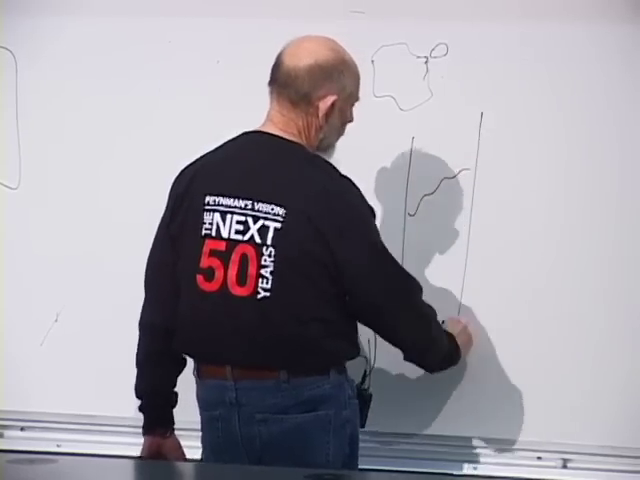
\includegraphics[width=0.72\textwidth]{lecture_06_figure_03.png}\caption{Die vervollständigten Austauschschaubilder an der Tafel: Bei der Emission tritt ein Kopplungsfaktor auf und bei der Absorption erneut.}\lectureframe{00:11:30.000}\end{figure}

In der Stringtheorie wird das Photon durch ein Graviton und die elektrische Ladung durch \(g_s\) ersetzt. Ein Faktor gehört zur Emission, ein weiterer zur Absorption, sodass die Stärke der Gravitation mit \(g_s^2\) skaliert.

Bei großen Abständen muss dieselbe Wechselwirkung das Newtonsche Kraftgesetz reproduzieren,
\begin{equation}
F_{\mathrm{grav}}\sim G_N\frac{M_1M_2}{r^2}.
\end{equation}
Die Massen und die Abhängigkeit vom inversen Quadrat beschreiben die Quellen und die Ausbreitung; hier kommt es auf die Kopplung an, die sie multipliziert.

\begin{figure}[htbp]\centering
\begin{tikzpicture}[x=1cm,y=1cm]
  \node[font=\small\bfseries] at (1.8,3.55) {electromagnetism};
  \draw[line width=0.8pt] (0,0) -- (0,3);
  \draw[line width=0.8pt] (3.6,0) -- (3.6,3);
  \draw[line width=0.8pt] plot[smooth] coordinates {(0,1.5) (0.45,1.72) (0.9,1.28) (1.35,1.72) (1.8,1.28) (2.25,1.72) (2.7,1.28) (3.15,1.72) (3.6,1.5)};
  \node[below] at (0,1.42) {\(e\)};
  \node[below] at (3.6,1.42) {\(e\)};
  \node[font=\small] at (1.8,0.25) {exchange strength \(\propto e^2\)};
  \node[font=\small\bfseries] at (7.2,3.55) {string gravity};
  \draw[line width=0.8pt,rounded corners=6pt] (5.4,0) -- (5.2,0.7) -- (5.5,1.5) -- (5.25,2.3) -- (5.4,3);
  \draw[line width=0.8pt,rounded corners=6pt] (9,0) -- (9.2,0.7) -- (8.9,1.5) -- (9.15,2.3) -- (9,3);
  \draw[line width=0.8pt] plot[smooth] coordinates {(5.5,1.5) (5.95,1.72) (6.4,1.28) (6.85,1.72) (7.3,1.28) (7.75,1.72) (8.2,1.28) (8.65,1.72) (8.9,1.5)};
  \node[below] at (5.5,1.42) {\(g_s\)};
  \node[below] at (8.9,1.42) {\(g_s\)};
  \node[font=\small] at (7.2,0.25) {exchange strength \(\propto g_s^2\)};
\end{tikzpicture}\caption{Die Analogie beim Abzählen der Kopplungsfaktoren. Jedes Ende des ausgetauschten Quants trägt einen Wechselwirkungsfaktor bei.}\end{figure}

Diese Beobachtung legt die Newton-Konstante beinahe fest. Die Kopplung \(g_s\) ist dimensionslos, während \(G_N\) in vier Dimensionen die Dimension einer Länge zum Quadrat hat. Die verfügbare mikroskopische Länge ist \(\ell_s\), also gilt
\begin{equation}
G_N\sim g_s^2\ell_s^2.
\label{eq:l06-newton-string}
\end{equation}
Zusammen mit Gleichung~\eqref{eq:l06-planck-area} folgt
\begin{equation}
\ell_p\sim g_s\ell_s.
\label{eq:l06-planck-string}
\end{equation}

\begin{figure}[htbp]\centering
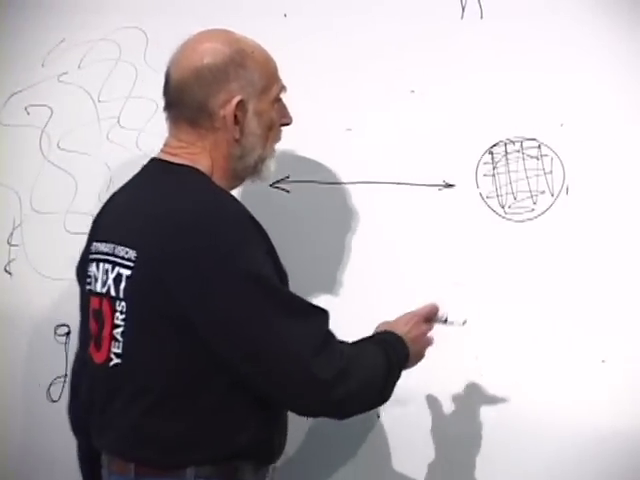
\includegraphics[width=0.72\textwidth]{lecture_06_figure_04.png}\caption{Die grundlegenden Beziehungen an der Tafel: \(\ell_p^2=G_N\) und \(\ell_p\sim g_s\ell_s\).}\lectureframe{00:15:45.000}\end{figure}

Gleichung~\eqref{eq:l06-newton-string} ist der vereinfachte Zusammenhang, den wir in dieser Vorlesung durchgehend verwenden.\editorialnote{In einer kompaktifizierten Stringtheorie hängt die effektive vierdimensionale Newton-Konstante auch vom Kompaktifizierungsvolumen und von Konventionen mit Faktoren der Größenordnung eins ab. Die Vorlesung lässt diese Größen außer Acht, um die Skalierung der Korrespondenz herauszuarbeiten.}

\begin{classroomqa}\audiencequestion{Ist \(g_s\) größer oder kleiner als eins, und welche Länge ist größer?\lecturetimestamp{00:16:00}}\lecturerresponse{Wir arbeiten bei schwacher Kopplung, \(g_s<1\). Dann bedeutet \(\ell_p\sim g_s\ell_s\), dass die Stringlänge größer als die Planck-Länge ist. Starke Kopplung erfordert eine andere Beschreibung, die wir hier nicht benötigen.}\end{classroomqa}

\section{Die Zählung für Schwarze Löcher}

Unter Weglassung der Boltzmann-Konstante und numerischer Faktoren lautet die Bekenstein--Hawking-Entropie
\begin{equation}
S_{\mathrm{BH}}=\frac{A}{4G_N}sim\frac{A}{G_N}sim\frac{A}{\ell_p^2}.
\label{eq:l06-bh-area}
\end{equation}
Der Faktor \(1/4\) ist in der semiklassischen Formel exakt, spielt für dieses Skalierungsargument aber keine Rolle.

\begin{classroomqa}\audiencequestion{Steht der Index ``BH'' für Schwarzes Loch oder für Bekenstein--Hawking?\lecturetimestamp{00:16:51}}\lecturerresponse{Für unsere Zwecke kann er an beides erinnern. Entscheidend ist die Aussage, dass die Entropie der Horizontfläche, gemessen in Planck-Flächen, entspricht.}\end{classroomqa}

Für ein vierdimensionales Schwarzschild-Schwarzes-Loch gilt
\begin{equation}
R_s=2G_NM,
\qquad
A=4\pi R_s^2.
\end{equation}
Lassen wir, wie in der Vorlesung, \(2\) und \(4\pi\) weg,
\begin{align}
S_{\mathrm{BH}}
&\sim \frac{R_s^2}{G_N}
\sim \frac{(G_NM)^2}{G_N} \\
&\sim M^2G_N
\sim M^2\ell_p^2.
\label{eq:l06-bh-mass}
\end{align}
Dies ist die Form, die wir mit einer Stringzählung vergleichen werden.

\section{Eine lange Saite als Zufallsweg}

Wir beginnen mit einer kurzen Saite und führen ihr Energie zu. Eine typische hoch angeregte Saite bleibt keine ordentliche Schleife. Sie wird zu einem langen, verwickelten Objekt – wie eine Angelschnur, die sich auf einer verhedderten Rolle verknotet hat. Dieses Knäuel besitzt Entropie, weil es enorm viele Konfigurationen gibt, die makroskopisch gleich aussehen.

Um sie zu zählen, ersetzen wir den Raum durch ein Gitter mit Kanten der Länge \(\ell_s\). Die Ecken sind die Gitterpunkte, die Kanten die Linien und die elementaren Quadrate die Flächen. Eine Saite wird als zusammenhängende Folge von Kanten dargestellt. Dieses Modell ist bewusst grob, doch seine exponentielle Zustandszahl erfasst die gesuchte Skalierung.

\begin{figure}[htbp]\centering
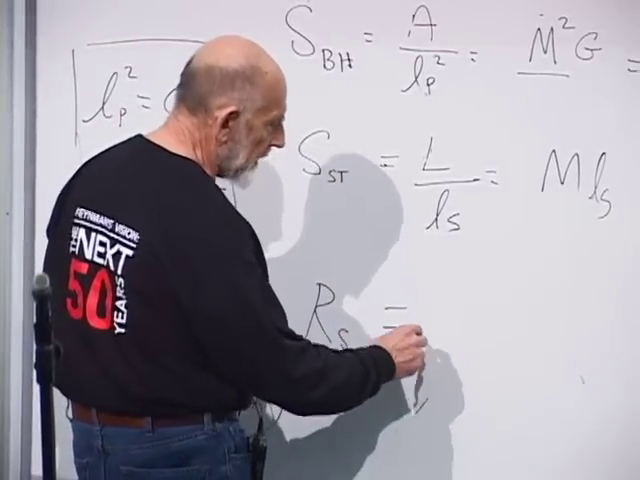
\includegraphics[width=0.72\textwidth]{lecture_06_figure_05.png}\caption{Das zweidimensionale Gittermodell. Das blaue Segment markiert einen Schritt der Saite; an jedem Gitterpunkt werden die vier möglichen Fortsetzungen gezählt.}\lectureframe{00:23:50.000}\end{figure}

\begin{classroomqa}\audiencequestion{Wie viele Wahlmöglichkeiten gibt es bei jedem Schritt des Modellwegs?\lecturetimestamp{00:22:43}}\lecturerresponse{Auf dem quadratischen Gitter sind es vier, da unmittelbares Zurückgehen erlaubt ist. In drei Dimensionen wären es sechs. Bei einem anderen Gitter ändert sich die konkrete Zahl, nicht aber die Tatsache, dass die Zahl der Wege exponentiell mit der Anzahl der Kanten wächst.}\end{classroomqa}

Hat die Saite \(n\) Kanten, so ergibt sich für das zweidimensionale Modell die Zählung
\begin{equation}
\Omega_n\sim4^n.
\label{eq:l06-walk-count}
\end{equation}
Es gibt einen einzigen Ausnahmefall, den geradlinigen Weg, aber das ist nur ein Zustand unter \(4^n\). Ein typischer Weg faltet sich wiederholt und füllt ein verwickeltes Knäuel aus. Für große \(n\) sieht fast jede zufällig erzeugte Konfiguration qualitativ wie jede andere aus.

Die Entropie ist der Logarithmus der Anzahl makroskopisch ununterscheidbarer Konfigurationen:
\begin{equation}
S_{\mathrm{st}}=\log\Omega_n\sim n\log4\sim n.
\label{eq:l06-string-entropy-n}
\end{equation}

\begin{classroomqa}\audiencequestion{Warum ist die Entropie proportional zu \(n\) und nicht zu \(4^n\)?\lecturetimestamp{00:25:39}}\lecturerresponse{Die Entropie ist der Logarithmus der Zustandszahl. Also gilt \(\log(4^n)=n\log4\); den Faktor \(\log4\), eine Konstante der Größenordnung eins, lassen wir weg.}\end{classroomqa}

Ist \(L\) die Länge entlang der Saite, gemessen von einem Ende bis zum anderen, so gilt
\begin{equation}
n=\frac{L}{\ell_s},
\qquad
S_{\mathrm{st}}\sim\frac{L}{\ell_s}.
\label{eq:l06-string-entropy-length}
\end{equation}
Hier ist \(L\) nicht der Durchmesser des verwickelten Knäuels. Gemeint ist die viel größere Strecke entlang der Saite.

Als Nächstes ersetzen wir die Länge entlang der Saite durch die Masse. Bei \(c=\hbar=1\) hat die Masse die Dimension einer inversen Länge. Eine Kante von der Größe einer Stringlänge trägt daher eine Masse der Größenordnung
\begin{equation}
m_{\mathrm{link}}\sim\frac{1}{\ell_s}.
\label{eq:l06-link-mass}
\end{equation}

\begin{classroomqa}\audiencequestion{Warum muss die Masse einer Kante mit \(1/\ell_s\) skalieren?\lecturetimestamp{00:29:20}}\lecturerresponse{In diesen Einheiten ist die Masse eine inverse Länge, und \(\ell_s\) ist die einzige verfügbare Länge. Äquivalent dazu ergibt eine Stringspannung der Größenordnung \(1/\ell_s^2\) multipliziert mit einer Kantenlänge \(\ell_s\) dasselbe Resultat.}\end{classroomqa}

Für die gesamte Saite gilt dann
\begin{equation}
M\sim n m_{\mathrm{link}}
\sim\frac{n}{\ell_s}
\sim\frac{L}{\ell_s^2},
\qquad
L\sim M\ell_s^2.
\label{eq:l06-string-mass}
\end{equation}
Einsetzen in Gleichung~\eqref{eq:l06-string-entropy-length} ergibt
\begin{equation}
S_{\mathrm{st}}\sim M\ell_s.
\label{eq:l06-string-entropy-mass}
\end{equation}
Der Gitterweg berücksichtigt weder die Zwangsbedingungen auf dem Weltblatt noch numerische Koeffizienten. Das exponentielle Wachstum des Spektrums hoch angeregter Saiten liefert jedoch dieselbe führende Skalierung.\editorialnote{Die Zufallsweg-Konstruktion dient als Merkhilfe für die Zustandsdichte der Saite bei hohen Anregungen; sie ist keine wörtliche Diskretisierung einer fundamentalen Saite.}

\section{Die Diskrepanz, die das Argument in Gang setzt}

Die beiden Ergebnisse lauten nun
\begin{equation}
S_{\mathrm{BH}}\sim M^2\ell_p^2,
\qquad
S_{\mathrm{st}}\sim M\ell_s.
\label{eq:l06-two-entropies}
\end{equation}
Sie ähneln einander, sind aber bei fester Masse und beliebiger Kopplung nicht gleich. Der Ausdruck für das Schwarze Loch ist quadratisch in \(M\), der für die Saite linear. Wir können eine heiße Saite nicht einfach zum Schwarzen Loch erklären, ohne zu erläutern, wie die beiden Bereiche ineinander übergehen.

\begin{figure}[htbp]\centering
\includegraphics[width=0.78\textwidth]{lecture_06_figure_06.png}\caption{Der ungehinderte Vergleich an der Tafel: oben die Entropie des Schwarzen Lochs, unten die der langen Saite; links die Beziehungen zwischen Planck- und Stringlänge.--}\lectureframe{00:33:20.000}\end{figure}

Hier legte die Vorlesung eine Pause ein. Die Spannung ist nützlich: Die Diskrepanz widerlegt die Idee nicht, sondern ist der Hinweis darauf, dass wir denselben Zustand vergleichen müssen, während wir die Stärke der Gravitation verändern.

\section{Den Kopplungsregler drehen}

Wir halten \(\ell_s\) fest und stellen uns vor, \(g_s\) lasse sich verändern. Bei \(g_s=0\) spalten sich Strings weder auf noch vereinigen sie sich, und die Gravitation verschwindet, weil \(G_N\sim g_s^2\ell_s^2\). Ein hinreichend energiereicher Zustand ist dann eine lange, schwach wechselwirkende Saite.

Wir erhöhen \(g_s\) langsam. Stringwechselwirkungen werden möglich, und – wichtiger für das gegenwärtige Argument – die Gravitation wird stärker.

\begin{classroomqa}\audiencequestion{Ist der erste Effekt einer Zunahme von \(g_s\) einfach, dass sich die Saite in kürzere Saiten aufspaltet?\lecturetimestamp{00:36:29}}\lecturerresponse{Aufspaltungen und Vereinigungen werden möglich. Wir halten aber \(\ell_s\) fest und verfolgen den Zustand hoher Entropie. Entscheidend ist, dass \(G_N\) wächst und damit die Eigengravitation der langen Saite das verwickelte Knäuel zusammenzieht.}\end{classroomqa}

Das Objekt zieht sich zusammen und wird dichter. Seine gravitative potenzielle Energie ist negativ; durch die Kontraktion sinkt daher seine Gesamtenergie und folglich seine Masse.

\begin{classroomqa}\audiencequestion{Nimmt die Energie zu oder ab, wenn die Eigengravitation die Saite zusammenzieht?\lecturetimestamp{00:37:48}}\lecturerresponse{Sie nimmt ab. Die Bindungsenergie wird negativer. Die Masse entlang dieses Verlaufs muss nicht konstant bleiben, auch wenn wir weiterhin denselben Zustand verfolgen.}\end{classroomqa}

Schließlich ist die Größe des Objekts mit seinem Schwarzschild-Radius vergleichbar. Von da an ist die Beschreibung als Schwarzes Loch die natürliche. Eine größere anfängliche Anregung erreicht diesen Punkt bei geringerer Kopplung, denn für ein massereicheres Objekt ist weniger Gravitationsstärke erforderlich, um einen Horizont zu bilden.

\begin{figure}[htbp]\centering
\resizebox{0.95\linewidth}{!}{%
\begin{tikzpicture}[x=1cm,y=1cm,>=Latex]
  \draw[->,line width=0.9pt] (0,0) -- (11,0) node[right] {increasing \(g_s\)};
  \node[draw,rounded corners,align=center,minimum width=2.6cm,minimum height=1.15cm] at (1.8,1.5) {long excited string\\weak self-gravity};
  \node[draw,rounded corners,align=center,minimum width=2.6cm,minimum height=1.15cm] at (5.5,1.5) {correspondence point\\\(R_s\sim\ell_s\)};
  \node[draw,circle,align=center,minimum size=1.8cm] at (9.3,1.5) {black\\hole};
  \draw[->,line width=0.8pt] (3.15,1.5) -- (4.1,1.5) node[midway,above,font=\small] {contracts};
  \draw[->,line width=0.8pt] (6.9,1.5) -- (8.25,1.5);
  \node[font=\small,align=center] at (5.5,-0.65) {same family of states followed slowly;\\binding energy and mass may change};
\end{tikzpicture}}\caption{Der Korrespondenzpfad bei festem \(\ell_s\). Eine Umkehrung des Pfeils führt den Zustand des Schwarzen Lochs zurück in einen Zustand langer Saite.}\end{figure}

\begin{classroomqa}\audiencequestion{Sollen wir uns \(g_s\) zwischen null und eins vorstellen?\lecturetimestamp{00:40:18}}\lecturerresponse{Ja. Das Argument bleibt im Bereich schwacher Kopplung. Ist \(g_s\) sehr klein, muss der Zustand entsprechend massereich sein, bevor er zu einem Schwarzen Loch wird. Den schlecht kontrollierten Bereich \(g_s>1\) müssen wir nicht betreten.}\end{classroomqa}

Die langsame Änderung ist in diesem Gedankenexperiment reversibel.

\begin{classroomqa}\audiencequestion{Wenn wir die Kopplung wieder so weit verringern, dass die Gravitation das Schwarze Loch nicht mehr zusammenhalten kann, was wird dann daraus?\lecturetimestamp{00:41:37}}\lecturerresponse{Eine lange Saite. Bei verschwindender Gravitation muss alles in dieser Konstruktion durch Stringzustände beschrieben werden. Dreht man den Regler in die eine Richtung, wird die Saite auf das Schwarze Loch abgebildet; dreht man ihn zurück, wird das Schwarze Loch auf die Saite abgebildet.}\end{classroomqa}

Bei fester Gesamtenergie und in einem festen Volumen besteht die dominante Konfiguration hoher Entropie im Wesentlichen aus einer einzigen langen Saite und nicht aus einer enormen Zahl kurzer Saiten. Diese Aussage wird hier nicht hergeleitet. Sie ist ein Ergebnis der statistischen Mechanik von Strings nahe dem Hagedorn-Regime und wird später wieder aufgegriffen.

\section{Was ein äußerer Beobachter sieht}

Wo ist die Saite, wenn das Objekt als Schwarzes Loch beschrieben wird? In der Beschreibung von außen verschwindet sie nicht plötzlich. In der Schwarzschild-Zeit wird der scheinbare Horizontübertritt auf beliebig späte Zeiten verschoben. Daher werden die Stringfreiheitsgrade so dargestellt, als sammelten sie sich auf oder nahe dem Horizont an.

\begin{figure}[htbp]\centering
\includegraphics[width=0.72\textwidth]{lecture_06_figure_07.png}\caption{Der Vergleich an der Tafel zwischen einem makroskopischen Horizont, an dem Strukturen auf der Stringskala nur einen dünnen Flaum bilden, und einem kleineren Horizont, dessen Radius sich der Schleifenskala nähert.}\lectureframe{00:45:30.000}\end{figure}

Für \(R_s\gg\ell_s\) ist das Schwarze Loch makroskopisch, und die Strukturen auf der Stringskala bilden im Verhältnis zum Horizontradius nur eine dünne Schicht. Nähert sich der Radius \(\ell_s\), verliert die Unterscheidung zwischen einem glatten Schwarzen Loch und einer ausgedehnten Saite ihre Bedeutung. Dies ist eine Beschreibung von außen im Sinne des gestreckten Horizonts; sie darf nicht mit der koordinatenunabhängigen Behauptung verwechselt werden, einfallende Materie überquere niemals einen regulären Horizont.\editorialnote{Die Vorlesung verwendet die Außenbeschreibung, die aus der Komplementarität Schwarzer Löcher vertraut ist. Die Formulierung ``am Horizont'' bezeichnet Freiheitsgrade, die in der Außenbeschreibung aufgelöst werden, und ist keine separate Herleitung ihres kovarianten Ortes.}

Der Übergang erfolgt bei
\begin{equation}
R_s\sim\ell_s.
\label{eq:l06-correspondence-radius}
\end{equation}
Unterhalb der Stringskala kann die Schwarzschild-Geometrie die Struktur, die sie tragen soll, nicht auflösen. Die Schleifen fluktuieren vom hypothetischen Horizont weg; der Zustand wird dann treffender als Saite bezeichnet.

\section{Der Korrespondenzpunkt}

Setzen wir \(R_s\sim G_NM\) in Gleichung~\eqref{eq:l06-correspondence-radius} ein:
\begin{equation}
G_NM\sim\ell_s.
\end{equation}
Dann setzen wir \(G_N\sim g_s^2\ell_s^2\) ein:
\begin{equation}
M g_s^2\ell_s^2\sim\ell_s,
\qquad
M g_s^2\ell_s\sim1.
\label{eq:l06-correspondence-condition}
\end{equation}

\begin{figure}[htbp]\centering
\includegraphics[width=0.72\textwidth]{lecture_06_figure_08.png}\caption{Die vollständige Übergangsrechnung an der Tafel: Aus \(R_s\sim\ell_s\) folgt die eingerahmte dimensionslose Bedingung \(Mg_s^2\ell_s\sim1\).}\lectureframe{00:49:50.000}\end{figure}

Ein Zuhörer bemerkte, worauf diese Bedingung hinausläuft. Am Korrespondenzpunkt gilt
\begin{align}
S_{\mathrm{BH}}
&\sim M^2\ell_p^2
\sim M^2g_s^2\ell_s^2 \\
&=(M\ell_s)(Mg_s^2\ell_s)
\sim M\ell_s
\sim S_{\mathrm{st}}.
\label{eq:l06-entropy-preview}
\end{align}

\begin{classroomqa}\audiencequestion{Folgt aus den Gleichungen bereits, dass die Entropien des Schwarzen Lochs und der Saite gleich werden?\lecturetimestamp{00:50:18}}\lecturerresponse{Ja. Genau darauf läuft die Rechnung hinaus. Die nötigen Bestandteile stehen an der Tafel, doch die Vorlesung setzt sie noch nicht vollständig zusammen, damit die Logik der Korrespondenz sorgfältig nachvollzogen werden kann.}\end{classroomqa}

Gleichung~\eqref{eq:l06-entropy-preview} ist die im Austausch angedeutete algebraische Vorschau in einer Zeile. Sie zeigt die Skalierung, nicht den exakten Koeffizienten \(1/4\). Für exakte mikroskopische Übereinstimmungen braucht man besser kontrollierbare Schwarze Löcher und detailliertere Stringkonstruktionen.\editorialnote{Die Vorlesung bricht ab, bevor Gleichung~\eqref{eq:l06-entropy-preview} als vollständige Herleitung präsentiert wird. Sie ist hier ausgeschrieben, weil das Publikum die Gleichheit ausdrücklich erkennt und alle dafür nötigen Beziehungen bereits eingeführt wurden.}

\section{Warum sich die Entropie mitnehmen lässt}

Ein logischer Baustein fehlt noch. Nehmen wir an, ein Steuerparameter wie ein Magnetfeld oder \(g_s\) werde hinreichend langsam variiert, während das System isoliert bleibt und sich reversibel entwickelt. Energien, Größen und Bindungsenergien können sich ändern, doch die Entropie bleibt erhalten:
\begin{equation}
\Delta S=0.
\label{eq:l06-adiabatic-entropy}
\end{equation}
Die Vorlesung verknüpft dies mit der Erhaltung von Information. Die Entropie misst die Information, die eine grobkörnige Beschreibung verbirgt; eine langsame, reversible Änderung des Hamiltonoperators ordnet die Zustände neu, ohne diese Information zu löschen.

\begin{classroomqa}\audiencequestion{Muss der Verlauf einen Phasenübergang vermeiden, damit die Entropie konstant bleibt?\lecturetimestamp{00:54:01}}\lecturerresponse{Ja, man muss den Zustand stetig verfolgen können. Ein endliches System hat keinen strikt nichtanalytischen thermodynamischen Phasenübergang wie im unendlichen Volumen. Ist die Änderung langsam genug, lässt sich die Korrespondenz als glatter Übergang behandeln.}\end{classroomqa}

Adiabatisch wird hier im stärkeren Sinn von quasistatisch und reversibel verwendet. Bei einem adiabatischen, aber irreversiblen Prozess kann Entropie entstehen; entscheidend sind die Langsamkeit und die Möglichkeit, den Zustand zu verfolgen.\editorialnote{Die thermodynamische Aussage \(\Delta S=0\) setzt einen reversiblen adiabatischen Verlauf voraus. In der Quantenmechanik entspricht dem die Idee, dieselbe Menge von Zuständen zu verfolgen, während sich ein Parameter ändert, ohne dass unkontrollierte Übergänge zwischen Energieniveaus auftreten.}

\begin{classroomqa}\audiencequestion{Warum hat eine einzige lange Saite mehr Entropie als mehrere kürzere Saiten mit derselben Gesamtmasse?\lecturetimestamp{00:54:44}}\lecturerresponse{Das ist kontraintuitiv, doch die explizite Zustandszählung bei hoher Energie bevorzugt in einem festen Volumen eine Komponente aus einer langen Saite. Der Beweis wird zurückgestellt; für das gegenwärtige Argument genügt uns, dass das Schwarze Loch auf den Sektor der Saite mit maximaler Entropie abgebildet wird und nicht auf ein verdünntes Gas aus sehr vielen kurzen Saiten.}\end{classroomqa}

Die Vorgehensweise ist daher:
\begin{enumerate}\item Wir beginnen mit einem Schwarzen Loch der Masse \(M_0\) bei der Kopplung \(g_{s,0}\).
\item Wir verringern \(g_s\) langsam und verfolgen dabei dieselbe Familie von Zuständen hoher Entropie.
\item Wir halten bei \(R_s\sim\ell_s\) an, wo die Beschreibung als Schwarzes Loch in die Beschreibung als lange Saite übergeht.
\item Wir zählen die Stringzustände mithilfe von \(S_{\mathrm{st}}\sim M\ell_s\).
\item Wir tragen diese Entropie auf dem reversiblen Weg zurück zum ursprünglichen Schwarzen Loch.
\end{enumerate}

\begin{figure}[htbp]\centering
\includegraphics[width=0.72\textwidth]{lecture_06_figure_09.png}\caption{Das Prinzip an der Tafel während der Erläuterung der Vorgehensweise: Eine adiabatische Änderung von \(g_s\) ändert \(S\) nicht.}\lectureframe{00:56:40.000}\end{figure}

Die Stringtheorie hat wesentlich genauere Entropiezählungen für geladene, rotierende, supersymmetrische, nahezu extremale und höherdimensionale Schwarze Löcher hervorgebracht. Die hier behandelte neutrale Schwarzschild-Lösung ist das grobe Korrespondenzargument: Sie identifiziert die parametrische Zustandsdichte und den physikalischen Übergang, aber keine exakte geschützte Entartung.\editorialnote{Die Übereinstimmung ist am stärksten bei speziellen Schwarzen Löchern, deren Zustandszählung bei Änderung der Kopplung geschützt bleibt. Diese Vorlesung gibt bewusst die einfachste Abschätzung der Größenordnung.}

\begin{classroomqa}\audiencequestion{Könnte der Zustand beim Abschalten der Gravitation zu zwei Strings werden statt genau zu einem?\lecturetimestamp{00:58:25}}\lecturerresponse{Für eine kleine Anzahl langer Strings gibt es eine endliche Wahrscheinlichkeit, und ob man einen oder zwei verwendet, ändert die führende Entropieskalierung nicht. Das Argument würde sich ändern, wenn der Zustand in ein großes Gas kurzer Strings zerfiele; die statistische Zählung bei hoher Energie bevorzugt dieses Ergebnis nicht.}\end{classroomqa}

Das Schwarze Loch besitzt die größte Entropie, die sich in einem Gebiet unterbringen lässt; die lange Saite ist der entsprechende Zustand hoher Entropie, wenn die Gravitation abgeschaltet wird. Diese beiden Beschreibungen sind nun miteinander verknüpft, aber noch nicht zu einer Präzisionsrechnung ausgebaut. Als Nächstes wiederholen wir die Rechnung sorgfältig und fragen, wie weit sich der Korrespondenz vertrauen lässt.

\chapter{Schwarze-Loch-Entropie, Holografie und de-Sitter-Raum}

\lectureoverview{Wir schließen das Korrespondenzargument ab, das in der vorherigen Vorlesung begonnen wurde. Die Entropie einer stark angeregten Saite ist proportional zu ihrer Masse, während die Entropie eines Schwarzschild-Schwarzen-Lochs proportional zu seiner Fläche ist. Die beiden Formeln werden nicht dadurch miteinander verknüpft, dass man ein stark gravitierendes Schwarzes Loch mit einer freien Saite gleichsetzt, sondern indem man die Stringkopplung langsam verändert, bis beide Beschreibungen zusammenpassen. Das Flächengesetz führt dann auf natürliche Weise zum holografischen Prinzip. Im letzten Teil der Vorlesung werden expandierender Raum und die de-Sitter-Geometrie eingeführt, deren Horizont in der nächsten Vorlesung untersucht wird.}

\section{Zurück zum Abzählproblem}

Bei der Abzählung langer Saiten war noch eine Frage offen. Wird eine feste Gesamtlänge auf mehrere Saiten verteilt, sind identische Saiten gleicher Länge ununterscheidbar. Ihre Positionen im Kasten gehören dennoch zum Zustand, und der Kasten wird ungefähr so groß gewählt wie der Bereich, den die entsprechende einzelne lange Saite einnimmt.

\begin{classroomqa}
\audiencequestion{Sind die kurzen Saiten voneinander unterscheidbar, und zählen ihre Positionen mit?\lecturetimestamp{00:00:37}}
\lecturerresponse{Saiten mit identischen Eigenschaften sind ununterscheidbar, ihre Positionen im Kasten werden jedoch mitgezählt. Der Vergleich erfolgt bei festem Volumen, das so gewählt ist, dass es dem von der langen Saite eingenommenen Bereich entspricht.}
\end{classroomqa}

Damit können wir nun das Ziel formulieren. Wir stellen eine kurze Liste von Gleichungen zusammen und leiten daraus die Skalierung der Schwarzen-Loch-Entropie ab. Dazu ist weder ein Integral noch eine unendliche Summe erforderlich. Die Schwierigkeit ist nicht algebraischer Art; sie besteht darin, zu erkennen, welche Größen miteinander verglichen werden dürfen und an welcher Stelle des Arguments.

\section{Natürliche Einheiten und die Planck-Fläche}

Wir setzen
\begin{equation}
c=\hbar=1,
\label{eq:l07-natural-units}
\end{equation}
, lassen aber die Newtonsche Gravitationskonstante explizit stehen. Daraus folgt zunächst, dass Zeit und Länge dieselbe Einheit haben. Die Photon-Beziehung
\begin{equation}
E=\frac{\hbar c}{\lambda}
\end{equation}
und die Masse-Energie-Beziehung \(E=mc^2\) ergeben dann
\begin{equation}
[M]=L^{-1}.
\label{eq:l07-mass-dimension}
\end{equation}
Masse lässt sich somit als inverse Länge angeben.

\begin{figure}[htbp]
\centering
\includegraphics[width=0.62\textwidth]{lecture_07_figure_02.png}
\caption{Die Konvention natürlicher Einheiten zu Beginn der Dimensionsbetrachtung. Die Energieformel wird durch die obigen Gleichungen ergänzt.}
\lectureframe{00:03:27.900}
\end{figure}

Um die Einheiten von \(G_N\) zu bestimmen, verwenden wir die Newtonsche Beschleunigung lediglich als Dimensionsbuchhaltung:
\begin{equation}
a\sim\frac{G_NM}{R^2}.
\end{equation}
Da \(T\) und \(L\) dieselben Einheiten haben, gilt \([a]=L/T^2=L^{-1}\). Zusammen mit Gleichung~\eqref{eq:l07-mass-dimension} folgt daraus
\begin{equation}
[G_N]=L^2.
\end{equation}
In diesen Einheiten hat die Newtonsche Gravitationskonstante die Dimension einer Fläche. Definiert man die Planck-Länge durch
\begin{equation}
G_N=\ell_p^2,
\label{eq:l07-planck-area}
\end{equation}
so wird unmittelbar klar, warum \(A/G_N=A/\ell_p^2\) dimensionslos ist: Der Ausdruck gibt eine Fläche in Planck-Flächen an.

\section{Die Stringkopplung und die Stärke der Gravitation}

Nun müssen wir die Gravitation in die Sprache der Stringtheorie übersetzen. Anschaulich lässt sich das als Austauschprozess auffassen. Wenn eine Saite sich selbst kreuzt, kann sie sich aufspalten und wieder verbinden. Eine kleine geschlossene Stringschleife kann von einem Objekt emittiert und von einem anderen absorbiert werden; handelt es sich bei dieser Anregung um ein Graviton, vermittelt der Prozess die Gravitation. Bei der Emission tritt ein Wechselwirkungsfaktor auf und bei der Absorption ein weiterer, sodass die Stärke des Austauschs den Faktor \(g_s^2\) enthält.

Die Kopplung \(g_s\) ist dimensionslos. Genauer gesagt ist sie eine Kopplung auf Amplitudenebene, während eine Wahrscheinlichkeit oder Rate in der Ordnung \(g_s^2\) beginnt.\editorialnote{In der Vorlesung wird \(g_s\) gelegentlich als Wahrscheinlichkeit bezeichnet und dann zu deren Quadratwurzel korrigiert. Die Störungskopplung gehört auf die Amplitudenebene.} Da \(G_N\) die Dimension einer Fläche hat, fehlt noch eine Längenskala. Diese liefert die fundamentale Stringlänge \(\ell_s\), die Skala einer elementaren Auslenkung der Saite:
\begin{equation}
G_N\sim g_s^2\ell_s^2,
\qquad
\ell_p\sim g_s\ell_s.
\label{eq:l07-planck-string}
\end{equation}

\begin{figure}[htbp]
\centering
\includegraphics[width=0.72\textwidth]{lecture_07_figure_05.png}
\caption{Die Kopplungsbeziehung an der Tafel: \(G_N=\ell_p^2\) und \(g_s^2\ell_s^2\sim\ell_p^2\).}
\lectureframe{00:12:15.000}
\end{figure}

Bei schwacher Kopplung, \(g_s\ll1\), ist die Planck-Länge viel kleiner als die Stringlänge. Wird \(g_s\) verringert, schwächt sich die Gravitation ab, während die elementare Stringskala unverändert bleibt.\editorialnote{In einer effektiven vierdimensionalen Theorie gehen auch Kompaktifizierungsdaten und numerische Konventionen in \(G_N\) ein. In diesem Skalierungsargument werden sie festgehalten und nicht weiter berücksichtigt.}

\section{Abzählung einer langen Saite}

Entropie zählt die elementaren Entscheidungen, die zur Festlegung eines Zustands erforderlich sind. Wir ersetzen eine stark angeregte Saite durch einen Weg auf einem quadratischen Gitter. An jedem Gitterpunkt kann der nächste Schritt in eine von vier Richtungen weisen. Ob man die elementare Wahl als eine Entscheidung zwischen vier Möglichkeiten oder als zwei binäre Entscheidungen beschreibt, ändert lediglich eine Konstante der Größenordnung eins. Entscheidend ist die Anzahl der Schritte.

Sei \(L\) die Konturlänge der Saite und \(\ell_s\) die Länge jedes Schritts. Dann sind
\begin{equation}
N=\frac{L}{\ell_s}
\end{equation}
Schritte erforderlich. Die Anzahl der Wege wächst exponentiell, schematisch wie \(\Omega_N\sim q^N\), wobei \(q\) von der Größenordnung eins ist. Daher gilt
\begin{equation}
S_{\mathrm{str}}=\log\Omega_N\sim N\sim\frac{L}{\ell_s}.
\label{eq:l07-string-entropy-length}
\end{equation}

\begin{figure}[htbp]
\centering
\includegraphics[width=0.68\textwidth]{lecture_07_figure_03.png}

\vspace{0.7em}
\begin{tikzpicture}[scale=0.82]
  \draw[step=0.8cm,gray!45,thin] (0,0) grid (6.4,4.0);
  \draw[very thick,blue!60!black]
    (0.8,0.8)--(1.6,0.8)--(1.6,1.6)--(2.4,1.6)--(2.4,2.4)--
    (3.2,2.4)--(3.2,1.6)--(4.0,1.6)--(4.0,2.4)--(4.8,2.4)--
    (4.8,3.2)--(5.6,3.2);
  \draw[<->,thick] (0.8,-0.35)--(1.6,-0.35);
  \node[below] at (1.2,-0.35) {step \(\ell_s\)};
  \node[align=center] at (8.1,2.0) {\(N=L/\ell_s\) steps\\[0.3em]\(S_{\mathrm{str}}\sim N\)};
\end{tikzpicture}
\caption{Das Gittermodell an der Tafel und seine bereinigte Interpretation als Zufallsweg. Die Konturlänge, nicht der Durchmesser des wirren Knäuels, bestimmt die Anzahl der Wahlmöglichkeiten.}
\lectureframe{00:17:20.000}
\end{figure}

Die Masse wird anhand derselben elementaren Segmente bestimmt. Ein Segment der Länge \(\ell_s\) hat die Massenskala
\begin{equation}
m_{\mathrm{seg}}\sim\frac{1}{\ell_s}.
\end{equation}

\begin{classroomqa}
\audiencequestion{Wird dem elementaren Segment die Länge \(\ell_s\) zugeordnet?\lecturetimestamp{00:18:56}}
\lecturerresponse{Ja. Seine charakteristische Länge ist \(\ell_s\), also ist seine charakteristische Masse in natürlichen Einheiten \(1/\ell_s\).}
\end{classroomqa}

Addiert man die Massen der \(L/\ell_s\) Segmente, erhält man
\begin{equation}
M\sim\frac{L}{\ell_s}\frac{1}{\ell_s}
=\frac{L}{\ell_s^2},
\qquad
L\sim M\ell_s^2.
\label{eq:l07-string-mass}
\end{equation}
Die kinetische und die potenzielle Energie der schwingenden Saite sind in dieser Skalierungsbeziehung zusammengefasst; eine ausführliche statistisch-mechanische Behandlung ergibt dieselbe Abhängigkeit. Einsetzen in Gleichung~\eqref{eq:l07-string-entropy-length} liefert die Stringformel, die wir benötigen:
\begin{equation}
S_{\mathrm{str}}\sim M\ell_s.
\label{eq:l07-string-entropy-mass}
\end{equation}

\begin{figure}[htbp]
\centering
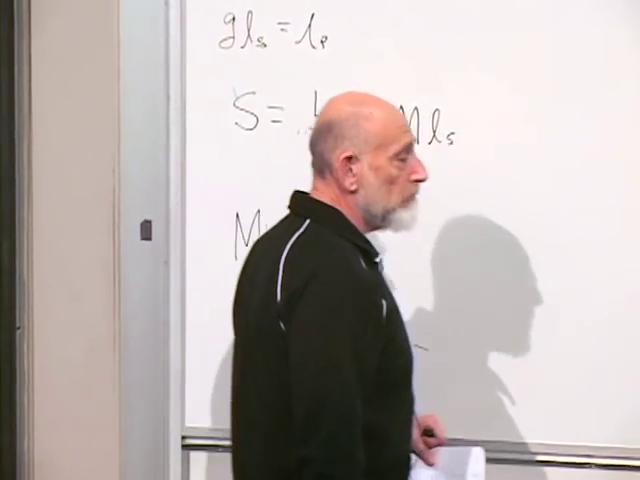
\includegraphics[width=0.66\textwidth]{lecture_07_figure_04.png}
\caption{Die Spalte für die Saite, zusammengestellt vor dem Vergleich: \(\ell_p\sim g_s\ell_s\), \(S_{\mathrm{str}}\sim L/\ell_s\sim M\ell_s\) und \(M\sim L/\ell_s^2\).}
\lectureframe{00:21:57.800}
\end{figure}

\section{Warum eine freie Saite noch kein Schwarzes Loch ist}

Auf der gravitativen Seite lautet die exakte semiklassische Formel
\begin{equation}
S_{\mathrm{BH}}=\frac{A}{4G_N}.
\label{eq:l07-bh-exact}
\end{equation}

\begin{classroomqa}
\audiencequestion{Welcher Zahlenfaktor gehört in den Nenner?\lecturetimestamp{00:23:28}}
\lecturerresponse{Vier. Das Korrespondenzargument wird die Skalierung reproduzieren, ist aber zu grob, um diesen exakten Faktor zu bestimmen.}
\end{classroomqa}

Für ein vierdimensionales Schwarzschild-Schwarzes-Loch gilt
\begin{equation}
R_s=2G_NM,
\qquad
A=4\pi R_s^2.
\end{equation}
Lässt man, wie in der Vorlesung, die numerischen Konstanten weg, erhält man
\begin{align}
S_{\mathrm{BH}}
&\sim\frac{A}{G_N}
\sim\frac{(G_NM)^2}{G_N} \\
&\sim M^2G_N
\sim M^2\ell_p^2.
\label{eq:l07-bh-scaling}
\end{align}

\begin{figure}[htbp]
\centering
\includegraphics[width=0.72\textwidth]{lecture_07_figure_06.png}
\caption{Der vollständige Vergleich an der Tafel: Die Stringentropie ist eine Länge in Stringeinheiten, während die Schwarze-Loch-Entropie eine Fläche in Planck-Einheiten ist.}
\lectureframe{00:25:35.000}
\end{figure}

Die Ähnlichkeit zwischen den Gleichungen~\eqref{eq:l07-string-entropy-mass} und \eqref{eq:l07-bh-scaling} ist suggestiv, doch es handelt sich nicht um dieselbe Formel. Es wäre falsch, das ursprüngliche Schwarze Loch einfach als freie Saite zu bezeichnen und die entsprechende Formel einzusetzen. Bei der Abzählung der freien Saite wird die anziehende Wechselwirkung zwischen ihren Teilen vernachlässigt – genau jene Wechselwirkung, die die Saite zu einem Schwarzen Loch zusammenzieht und durch negative Bindungsenergie ihre Gesamtenergie senkt.

Ein Stern macht diesen Fehler anschaulich. Ein heißes Gas mit der Masse eines Sterns in einem übergroßen Kasten ist kein Modell für einen Stern, selbst wenn die Temperatur gleich ist. Die Eigengravitation verändert die Gleichgewichtsgröße und den Zusammenhang zwischen Energie und Entropie. Jede Selbstwechselwirkung einer langen Saite einzeln zu berücksichtigen, wäre schwierig; deshalb werden wir darauf verzichten.

\begin{classroomqa}
\audiencequestion{Wenn eine kleine Schleife eine lange Saite verlässt, nimmt deren Entropie ab. Senkt der Gravitonenaustausch dann die Entropie des gravitierenden Systems?\lecturetimestamp{00:28:48}}
\lecturerresponse{Nicht beim hier betrachteten Gleichgewichtsaustausch. Virtuelle Anregungen werden in beide Richtungen emittiert und absorbiert; die Skizze zeigt keinen tatsächlichen Verlust eines dauerhaft abgespaltenen Saitenstücks. Sie soll hier lediglich die beiden Kopplungsfaktoren und damit die Abhängigkeit von \(g_s^2\) verdeutlichen.}
\end{classroomqa}

\section{Das adiabatische Korrespondenzspiel}

Beginnen wir stattdessen dort, wo die Gravitation vernachlässigbar ist. Bei \(g_s\to0\) kreuzen sich Saiten, ohne sich aufzuspalten oder zu verbinden, und die Eigengravitation verschwindet. Erhöhen wir \(g_s\) bei festgehaltenem \(\ell_s\), wird die Gravitation stärker, eine stark angeregte Saite zieht sich zusammen und wird schließlich zu einem Schwarzen Loch. Dreht man den Regler langsam zurück, muss das Schwarze Loch wieder in einen Stringzustand übergehen. Es kann sich in eine kleine Zahl langer Saiten verwandeln, doch die Hochenergie-Abzählung aus der vorherigen Vorlesung besagt, dass der dominante Sektor eine lange Saite und nicht ein riesiges Gas aus kurzen Saiten enthält.

\begin{classroomqa}
\audiencequestion{Was bleibt fest, während die Kopplung verändert wird?\lecturetimestamp{00:32:19}}
\lecturerresponse{Die Stringlänge \(\ell_s\) und damit die elementare Stringmassenskala \(1/\ell_s\) bleiben fest. Der Regler verändert \(g_s\) und damit \(G_N\sim g_s^2\ell_s^2\).}
\end{classroomqa}

Die Änderung muss langsam, isoliert und reversibel sein. Unter diesen Bedingungen ist die Entropie eine adiabatische Invariante:
\begin{equation}
\Delta S=0.
\label{eq:l07-adiabatic}
\end{equation}
Allein die Langsamkeit reicht nicht aus, wenn dissipative oder unkontrollierte Übergänge auftreten. Hier bedeutet ``adiabatisch'', dass sich dieselbe Zustandsfamilie kontinuierlich verfolgen lässt.\editorialnote{Dies ist der reversible thermodynamische Sinn von adiabatisch. Ein irreversibler Prozess kann im Sinne eines fehlenden Wärmeaustauschs adiabatisch sein und dennoch Entropie erzeugen.}

Sei die Masse des betrachteten Schwarzen Lochs \(M_0\) und seine Kopplung \(g_{s,0}\). Bevor wir das Flächengesetz verwenden, das wir erklären wollen, sagt die Dimensionsanalyse lediglich, dass die Entropie eines neutralen, nicht rotierenden Schwarzen Lochs eine Funktion der dimensionslosen Kombination
\begin{equation}
S_{\mathrm{BH}}=f(M\ell_p)
=f(Mg_s\ell_s).
\label{eq:l07-entropy-function}
\end{equation}
ist.
Bei festem \(\ell_s\) bleibt auf einem isentropen Pfad daher
\begin{equation}
Mg_s=M_0g_{s,0}
\label{eq:l07-adiabat}
\end{equation}
konstant, sofern derselbe Zustandszweig verfolgt wird.

Wenn \(g_s\) abnimmt, wird negative Bindungsenergie abgeführt, sodass die Masse \(M\) entlang dieses Pfads zunimmt. Auch die zugrunde liegende Stringkonfiguration ist weniger stark gebunden und breitet sich aus. Der formale Schwarzschildradius verhält sich auf der Adiabate jedoch wie \(R_s\sim Mg_s^2\ell_s^2\sim g_s\ell_s\) und nimmt daher ab.\editorialnote{Die mündliche Erläuterung verwendet ``wächst'' für das Objekt, das aus der gravitativen Bindung gelöst wird. Dies sollte nicht so verstanden werden, als nähme der Schwarzschildradius entlang der hergeleiteten Adiabate zu.}

\begin{classroomqa}
\audiencequestion{Wächst oder schrumpft das Objekt, wenn die Gravitation schwächer wird?\lecturetimestamp{00:36:28}}
\lecturerresponse{Seine Stringstruktur wird freigesetzt und breitet sich aus, während seine Masse zunimmt, weil die negative Bindungsenergie abgebaut wird. Der nach der Formel für Schwarze Löcher bestimmte Radius nimmt ab, bis er die Stringskala erreicht; dann ist diese Beschreibung als Schwarzes Loch nicht mehr brauchbar.}
\end{classroomqa}

\section{Zwei Kurven und ihr Schnittpunkt}

Tragen wir die Masse auf der vertikalen und die Stringkopplung auf der horizontalen Achse auf. Gleichung~\eqref{eq:l07-adiabat} beschreibt eine Hyperbel: \(M\propto g_s^{-1}\).

\begin{classroomqa}
\audiencequestion{Welche Kurve hat ein konstantes Produkt \(Mg_s\)?\lecturetimestamp{00:44:08}}
\lecturerresponse{Eine Hyperbel. Sie ist die Adiabate durch den Zielpunkt \((g_{s,0},M_0)\).}
\end{classroomqa}

Die zweite Kurve markiert den Übergang zwischen den Beschreibungen. Ein Schwarzes Loch lässt sich nicht mehr als gewöhnliche Schwarzschild-Geometrie auflösen, sobald sein Radius kleiner ist als eine elementare Auslenkung der Saite. Daher schätzen wir den Korrespondenzpunkt durch
\begin{equation}
R_s\sim\ell_s.
\label{eq:l07-correspondence-radius}
\end{equation}
Mit \(R_s\sim MG_N\) und Gleichung~\eqref{eq:l07-planck-string} wird daraus
\begin{equation}
Mg_s^2\ell_s^2\sim\ell_s,
\qquad
Mg_s^2\sim\frac{1}{\ell_s}.
\label{eq:l07-transition-curve}
\end{equation}
Die Übergangskurve fällt also wie \(M\propto g_s^{-2}\) und damit steiler als die Adiabate.

\begin{figure}[htbp]
\centering
\includegraphics[width=0.70\textwidth]{lecture_07_figure_07.png}

\vspace{0.6em}
\begin{tikzpicture}[x=1cm,y=0.78cm]
  \draw[->] (0.4,0.4)--(7.0,0.4) node[right] {\(g_s\)};
  \draw[->] (0.4,0.4)--(0.4,6.5) node[above] {\(M\)};
  \draw[thick,black] plot[smooth] coordinates {(1.0,5.6) (1.5,4.0) (2.2,2.9) (3.2,2.1) (4.6,1.55) (6.3,1.2)};
  \draw[very thick,red!70!black] plot[smooth] coordinates {(1.25,6.0) (1.55,4.55) (2.0,3.15) (2.7,2.0) (3.8,1.25) (5.8,0.78)};
  \fill (2.05,3.1) circle (2pt) node[above right] {\((g_{s,*},M_*)\)};
  \node[black,rotate=-17] at (4.75,1.9) {\(Mg_s=M_0g_{s,0}\)};
  \node[red!70!black,rotate=-25] at (4.45,0.95) {\(Mg_s^2=1/\ell_s\)};
  \node at (5.75,3.5) {black hole};
  \node at (1.15,1.25) {string};
\end{tikzpicture}
\caption{Das Diagramm an der Tafel und seine bereinigte Interpretation. Die schwarze Adiabate schneidet die steiler verlaufende rote Korrespondenzkurve an dem Punkt, an dem das Objekt stringartig wird.}
\lectureframe{00:49:35.000}
\end{figure}

Am Schnittpunkt \((M_*,g_{s,*})\) lauten die beiden Gleichungen
\begin{align}
M_*g_{s,*} &= M_0g_{s,0}, \\
M_*g_{s,*}^2 &\sim \frac{1}{\ell_s}.
\end{align}
Wir quadrieren die erste Gleichung und dividieren durch die zweite:
\begin{equation}
M_*
\sim M_0^2g_{s,0}^2\ell_s.
\end{equation}
Multiplizieren wir mit \(\ell_s\), so erhalten wir
\begin{equation}
M_*\ell_s
\sim M_0^2g_{s,0}^2\ell_s^2
\sim M_0^2G_{N,0}.
\label{eq:l07-crossover-result}
\end{equation}

\begin{figure}[htbp]
\centering
\includegraphics[width=0.68\textwidth]{lecture_07_figure_08.png}
\caption{Die abgeschlossene Rechnung für den Übergang, einschließlich \(M_*\ell_s=M_0^2g_{s,0}^2\ell_s^2=M_0^2G_{N,0}\).}
\lectureframe{00:54:40.000}
\end{figure}

\begin{classroomqa}
\audiencequestion{Wenn man die beiden Kurvengleichungen dividiert, steht \(\ell_s\) dann im Zähler oder im Nenner?\lecturetimestamp{00:52:41}}
\lecturerresponse{Im Zähler. Die Division durch \(1/\ell_s\) ist eine Multiplikation mit \(\ell_s\). Daher gilt \(M_*\sim M_0^2g_{s,0}^2\ell_s\).}
\end{classroomqa}

Am Übergangspunkt gilt die Stringformel, also
\begin{equation}
S_*\sim M_*\ell_s.
\end{equation}
Die Entropie hat sich entlang des Pfads nicht verändert. Zusammen mit Gleichung~\eqref{eq:l07-crossover-result} ergibt sich daraus die Entropie des ursprünglichen Ziel-Schwarzen-Lochs:
\begin{equation}
S_{\mathrm{BH}}(M_0)
\sim M_0^2G_{N,0}
\sim M_0^2\ell_{p,0}^2.
\label{eq:l07-final-correspondence}
\end{equation}
Dies ist die gesuchte Flächengesetz-Skalierung.

\section{Was die Korrespondenz beweist und was nicht}

Diese Konstruktion besagt nicht, dass das ursprüngliche, stark gravitierende Schwarze Loch eine freie Saite ist. Sie führt das Objekt in einen Bereich, in dem die String-Abzählung verlässlich ist, bestimmt dort die Entropie und überträgt sie entlang eines reversiblen Pfads zurück. Der Übergang ist ein Crossover und keine scharf lokalisierte Phasengrenze. Deshalb kann diese Abschätzung den Koeffizienten \(1/4\) in Gleichung~\eqref{eq:l07-bh-exact} nicht bestimmen.

Dieselbe Logik funktioniert in ihrer parametrischen Form dennoch auch für geladene Schwarze Löcher, Schwarze Objekte in anderen Dimensionen und ausgedehnte Schwarze Branen. In Beispielen mit mehr Symmetrie und Supersymmetrie sind geschützte Zustandsabzählungen möglich, die bei veränderlicher Kopplung exakte Informationen bewahren. Solche Methoden liefern auch die numerischen Koeffizienten, erfordern aber mathematische Hilfsmittel, die für das vorliegende konzeptionelle Argument nicht nötig sind.

Vor allem liefert die Rechnung eine mikroskopische Deutung. Entropie ist ein Hinweis auf verborgene Struktur. Die Strömungsmechanik beschreibt Dichte, Druck und Strömung, ohne Moleküle zu berücksichtigen; die Entropie des Fluids zeigt, dass solche mikroskopischen Freiheitsgrade existieren. Allgemeine Relativitätstheorie beschreibt den Horizont ebenfalls, ohne seine Mikrozustände darzustellen. Die String-Abzählung zeigt, dass eine konsistente Quantentheorie der Gravitation genügend Zustände enthalten kann, um die Schwarze-Loch-Entropie zu erklären.

\begin{classroomqa}
\audiencequestion{Was hätte \(S\sim M^3\ell_p^3\) statt des quadratischen Ergebnisses bedeutet?\lecturetimestamp{00:59:41}}
\lecturerresponse{Das hätte wie ein Volumengesetz ausgesehen. Die Entropie gewöhnlicher Materie in einem Raum oder in einer Tasse Kaffee ist proportional zum Volumen. Das quadratische Ergebnis ist besonders, weil es über \(R_s\sim M\ell_p^2\) proportional zur Horizontfläche ist.}
\end{classroomqa}

Das Ergebnis ist ein Hinweis darauf, dass die Bekenstein--Hawking-Entropie nicht bloß eine formale thermodynamische Analogie ist. Sie deutet auf mikroskopische gravitative Freiheitsgrade hin, auch wenn die elementare Herleitung diese Freiheitsgrade nicht einzeln sichtbar macht.

\section{Von der maximalen Entropie zur Holografie}

Nun stellen wir eine andere Frage. Statt nach der Entropie eines bestimmten Zustands zu fragen, fragen wir nach der größtmöglichen Entropie, die mit einem Gebiet vereinbar ist.

Wir beginnen mit einem gewöhnlichen Gittermodell eines Raums. Wir unterteilen das Volumen in Zellen mit dem Volumen \(V_{\mathrm{cell}}\) und ordnen jeder Zelle eine Ja-Nein-Frage zu: besetzt oder leer. Susskind gibt dem imaginären Atom den bewusst absurden Namen ``''meatonium, damit keine realistischen atomaren Details von der Abzählung ablenken. Wenn
\begin{equation}
N=\frac{V}{V_{\mathrm{cell}}},
\end{equation}
gilt, sind die Anzahl der Konfigurationen und die maximale Entropie
\begin{equation}
\Omega=2^N,
\qquad
S_{\max}=\log\Omega=N\log2
\sim\frac{V}{V_{\mathrm{cell}}}.
\label{eq:l07-volume-count}
\end{equation}

\begin{figure}[htbp]
\centering
\includegraphics[width=0.68\textwidth]{lecture_07_figure_09.png}
\caption{Der Raum ist in Zellen mit je zwei Zuständen unterteilt. Damit wird eine maximale Entropie gezählt, nicht die Entropie des ordentlichen Raums, in dem die Vorlesung stattfindet.}
\lectureframe{01:05:20.000}
\end{figure}

Der tatsächliche Raum liegt weit unterhalb dieses Maximums. Ein Zustand, der all diese Zellmöglichkeiten chaotisch ausschöpfte, wäre extrem heiß. Aus dem Spielzeugmodell bleibt die gewöhnliche Erwartung, dass die Anzahl unabhängiger Freiheitsgrade und damit die maximale Entropie mit dem Volumen skaliert.

Die Gravitation stellt diese Erwartung auf den Kopf. Betrachten wir ein kugelförmiges Gebiet mit der Randfläche \(A\), der Anfangsentropie \(S_{\mathrm{i}}\) und der Masse \(M\), die kleiner ist als die Masse \(M_{\mathrm{BH}}\) eines Schwarzen Lochs, das die Kugel gerade ausfüllen würde. Wäre \(M\) größer, reichte sein Horizont bereits über den gewählten Rand hinaus.

Nun schicken wir eine Hülle mit der Masse \(M_{\mathrm{BH}}-M\) hinein. Ihre Zusammensetzung ist unerheblich; laut Vorlesung kann sie aus Licht, gewöhnlicher Materie oder sogar Schweizer Käse bestehen. Wir lassen sie kollabieren. Im Endzustand entsteht ein Schwarzes Loch, dessen Horizont das Gebiet gerade ausfüllt und dessen Entropie
\begin{equation}
S_{\mathrm{f}}=\frac{A}{4G_N}.
\end{equation}
beträgt. Der zweite Hauptsatz verlangt
\begin{equation}
S_{\mathrm{i}}\le S_{\mathrm{f}}
=\frac{A}{4G_N}.
\label{eq:l07-holographic-bound}
\end{equation}

\begin{figure}[htbp]
\centering
\includegraphics[width=0.70\textwidth]{lecture_07_figure_10.png}

\vspace{0.5em}
\begin{tikzpicture}[scale=0.88]
  \draw[thick] (0,0) circle (1.35);
  \draw[very thick,red!70!black] (0,0) circle (2.05);
  \fill[gray!25] (0,0) circle (1.32);
  \node at (0,0) {\(M,S_{\mathrm{i}}\)};
  \draw[-{Latex[length=3mm]},thick,red!70!black] (3.5,0)--(2.15,0);
  \node[align=center,right] at (3.5,0) {incoming shell\\\(M_{\mathrm{BH}}-M\)};
  \node[below] at (0,-2.2) {final horizon area \(A\)};
\end{tikzpicture}
\caption{Die Konstruktion mit der Hülle. Es wird genügend zusätzliche Masse nach innen geschickt, um ein Schwarzes Loch zu bilden, dessen Horizont das gewählte Gebiet gerade ausfüllt.}
\lectureframe{01:13:30.000}
\end{figure}

Da ein Schwarzes Loch dieser Größe ein zulässiger Zustand ist und die Ungleichung sättigt, ist die maximale Entropie
\begin{equation}
S_{\max}=\frac{A}{4G_N}.
\label{eq:l07-holographic-maximum}
\end{equation}
Dies ist das holografische Prinzip in seiner Zählform: Die maximale Anzahl unabhängiger Freiheitsgrade in einem gravitierenden Gebiet skaliert mit der Fläche seines Randes, ungefähr mit einem Freiheitsgrad der Größenordnung eins pro Planck-Fläche, und nicht mit der Anzahl der Planck-Volumina im Inneren.\editorialnote{Das Argument mit der Hülle setzt voraus, dass sich das Gebiet auf die beschriebene Weise einschließen und kollabieren lässt. Für allgemeinere Raumzeiten sind kovariante Entropiegrenzen erforderlich; das Kugelargument erfasst jedoch das in der Vorlesung verwendete Prinzip.}

Der Unterschied ist enorm. Die Intuition der lokalen Feldtheorie legt nahe, dass sich Wahlmöglichkeiten an verschiedenen inneren Punkten unabhängig kombinieren lassen, was zu einem Volumengesetz führen würde. Die Gravitation besagt, dass eine hinreichend große Zahl solcher Wahlmöglichkeiten selbst kollabieren würde; das Schwarze Loch liefert die größere zulässige Entropie. Die Zählung am Rand ist daher keine kleine Korrektur der Volumenzählung, sondern eine andere Organisation des Hilbert-Raums.

\begin{classroomqa}
\audiencequestion{Was geschieht in einem sehr großen Universum mit annähernd gleichmäßiger Dichte?\lecturetimestamp{01:15:48}}
\lecturerresponse{Diese Frage erfordert Kosmologie statt der statischen Kugelkonstruktion. Sie führt unmittelbar zu den expandierenden Lösungen der Einsteinschen Gleichungen.}
\end{classroomqa}

\begin{classroomqa}
\audiencequestion{Gibt es einen Zusammenhang zwischen der Flächengrenze und der Unschärferelation?\lecturetimestamp{01:16:03}}
\lecturerresponse{Die Vorlesung lässt diese Frage offen und wendet sich als Nächstes der Kosmologie zu.}
\end{classroomqa}

\section{Expandierender Raum}

Wir leiten die kosmologischen Lösungen der Einsteinschen Gleichungen hier nicht her, sondern schreiben sie hin und lernen, sie zu lesen. Räumliche Schnitte können positiv gekrümmt und geschlossen, negativ gekrümmt und hyperbolisch oder flach sein. Für die vorliegende Diskussion betrachten wir in einer zeitabhängigen Raumzeit räumliche, flache euklidische Schnitte.

\begin{classroomqa}
\audiencequestion{Was ist das Analogon des gewöhnlichen euklidischen Raums für die Raumzeit?\lecturetimestamp{01:19:37}}
\lecturerresponse{Der Minkowski-Raum. Die hier betrachtete Kosmologie hat flache räumliche Schnitte, ist aber keine Minkowski-Raumzeit, denn ihre räumliche Metrik ändert sich mit der Zeit.}
\end{classroomqa}

Das bekannte Bild eines Ballons beschreibt eine expandierende, geschlossene Fläche in einer Dimension weniger. Susskind erinnert sich an einen Versuch mit einem großen, markierten Ballon: Der Marker schwächte das Gummi, und der Ballon platzte mit einem Knall. Das Missgeschick macht auch einen begrifflichen Mangel der Analogie deutlich. Wenn ein gewöhnlicher Ballon expandiert, entfernen sich seine Gummimoleküle voneinander und das Material wird dünner, bis es reißt. Die lokalen Naturgesetze werden im kosmologischen Raum nicht verdünnt. Damit die Analogie erhalten bleibt, müsste man sich vorstellen, dass ständig neue Gummimoleküle eingefügt werden, sodass jede kleine Region dieselben lokalen Eigenschaften behält. In einem flachen Modell ersetzen wir den Ballon durch eine große Fläche, die gleichmäßig nach außen gezogen und auf ähnliche Weise fortlaufend ergänzt wird.

Mathematisch geht die Expansion in die Metrik ein:
\begin{equation}
\begin{aligned}
ds^2&=-dt^2+a(t)^2d\mathbf{x}^2,\\
d\mathbf{x}^2&=\delta_{ij}\,dx^i dx^j
=dx^2+dy^2+dz^2.
\end{aligned}
\label{eq:l07-frw-metric}
\end{equation}

\begin{figure}[htbp]
\centering
\includegraphics[width=0.72\textwidth]{lecture_07_figure_11.png}
\caption{Die räumlich flache Expansionsmetrik in der Form, in der sie an der Tafel angeschrieben wurde.}
\lectureframe{01:25:10.000}
\end{figure}

Punkte mit festen räumlichen Koordinaten heißen komovierend. Haben zwei solche Punkte den Koordinatenabstand \(\Delta x\), so beträgt ihr Eigenabstand zum Zeitpunkt \(t\)
\begin{equation}
D(t)=a(t)\Delta x.
\label{eq:l07-proper-distance}
\end{equation}
Ihre Koordinaten bewegen sich nicht, aber der metrische Abstand zwischen ihnen ändert sich. Leiten wir bei festem \(\Delta x\) ab, so erhalten wir
\begin{equation}
V=\dot D=\dot a\,\Delta x
=\frac{\dot a}{a}D.
\end{equation}
Wir definieren den Hubble-Parameter durch
\begin{equation}
H(t)=\frac{\dot a(t)}{a(t)}.
\label{eq:l07-hubble-parameter}
\end{equation}
Dann gilt
\begin{equation}
V=H(t)D,
\label{eq:l07-hubble-law}
\end{equation}
Dies ist das Hubble-Gesetz zu einem festen kosmischen Zeitpunkt.

\begin{figure}[htbp]
\centering
\includegraphics[width=0.68\textwidth]{lecture_07_figure_12.png}
\caption{Das Abstands-Rezessions-Gesetz für gleiche Zeiten an der Tafel: \(V=D\,\dot a/a\).}
\lectureframe{01:29:10.000}
\end{figure}

Die Bezeichnung ``''Hubble-Konstante kann irreführend sein. Im Allgemeinen ändert sich \(H(t)\) mit der Zeit. Räumlich konstant ist das Verhältnis \(V/D\) für jedes Paar komovierender Punkte auf derselben Zeitscheibe.

\begin{classroomqa}
\audiencequestion{Bei weit entfernten Galaxien: Auf welchen Zeitpunkt bezieht sich diese Relation? Wir beobachten sie zu einer früheren Epoche.\lecturetimestamp{01:31:10}}
\lecturerresponse{Gleichung~\eqref{eq:l07-hubble-law} ist eine Aussage für gleiche Zeiten. Eine Beobachtung folgt einem lichtartigen, in die Vergangenheit gerichteten Strahl und erfasst die entfernte Galaxie zu einem früheren Zeitpunkt. Der Zusammenhang zwischen gemessener Rotverschiebung und Entfernung erfordert daher die vollständige Geschichte entlang des Lichtkegels und nicht nur einen momentanen Wert von \(H\).}
\end{classroomqa}

\begin{figure}[htbp]
\centering
\includegraphics[width=0.66\textwidth]{lecture_07_figure_13.png}
\caption{Die Raumzeit-Skizze veranschaulicht den Unterschied zwischen einem Abstand zu gleicher Zeit und dem, was ein Beobachter entlang eines in die Vergangenheit gerichteten Lichtstrahls sieht.}
\lectureframe{01:33:20.000}
\end{figure}

\section{Die Hubble-Skala und die de-Sitter-Expansion}

In Einheiten mit \(c=1\) ergibt Gleichung~\eqref{eq:l07-hubble-law} für den Abstand
\begin{equation}
D_H=\frac{1}{H}.
\label{eq:l07-hubble-radius}
\end{equation}
eine Rezessionsgeschwindigkeit von eins. Komovierende Punkte in größerer Entfernung können \(V>1\) oder sogar \(V\gg1\) haben, ohne die spezielle Relativitätstheorie zu verletzen. Sie bewegen sich nicht schneller als Licht an einem lokalen Beobachter vorbei; ihr Eigenabstand wächst, weil die Geometrie dazwischen expandiert.\editorialnote{In einer allgemeinen zeitabhängigen Kosmologie ist \(1/H\) der Hubble-Radius und nicht automatisch ein Ereignishorizont. Im anschließend behandelten de-Sitter-Fall ist er die konstante Horizontskala.}

In vielen älteren, abgebremsten kosmologischen Modellen nimmt \(H(t)\) ab und \(1/H(t)\) zu, sodass Regionen, die sich einst überlichtschnell voneinander entfernten, später kausal in Kontakt treten können. Das in der Vorlesung besprochene Bild für späte Zeiten nähert sich stattdessen einem positiven konstanten Wert \(H\). Dann bleibt \(1/H\) fest, und die Expansionsgleichung lautet
\begin{equation}
\frac{\dot a}{a}=H,
\qquad
\dot a=Ha.
\label{eq:l07-constant-h}
\end{equation}

\begin{classroomqa}
\audiencequestion{Welche Einheit hat ein konstanter Hubble-Parameter?\lecturetimestamp{01:38:24}}
\lecturerresponse{Der Kehrwert einer Zeit. Bei \(c=1\) entspricht das dem Kehrwert einer Länge. Die Größe \(H^{-1}\) gibt sowohl eine Expansionszeit als auch eine Entfernungsskala an; in der Vorlesung dient etwa fünfzehn Milliarden Jahre als Größenordnungsbeispiel.}
\end{classroomqa}

Die Lösung von Gleichung~\eqref{eq:l07-constant-h} lautet
\begin{equation}
a(t)=a_0e^{Ht}.
\label{eq:l07-desitter-scale-factor}
\end{equation}

\begin{classroomqa}
\audiencequestion{Welche Funktion hat eine Änderungsrate, die proportional zu ihr selbst ist?\lecturetimestamp{01:39:04}}
\lecturerresponse{Eine Exponentialfunktion. Der Skalenfaktor ist also \(a_0e^{Ht}\), während der räumliche Koeffizient \(a(t)^2\) in der Metrik wie \(e^{2Ht}\) wächst.}
\end{classroomqa}

\begin{figure}[htbp]
\centering
\includegraphics[width=0.70\textwidth]{lecture_07_figure_14.png}
\caption{Die Gleichungen mit konstantem \(H\) und ihre exponentielle Lösung an der Tafel.}
\lectureframe{01:39:30.000}
\end{figure}

Eine Raumzeit mit dieser exponentiellen Expansion ist der de-Sitter-Raum. Seine konstante Hubble-Skala erzeugt einen Ereignishorizont in endlichem Eigenabstand. In gewissem Sinne bildet die Geometrie das Gegenstück zum Bild des Schwarzen Lochs: Ein Beobachter bleibt innerhalb eines kosmologischen Horizonts, während sich hinreichend weit entfernte Objekte entfernen und keine Signale senden können, die den Beobachter noch erreichen. Ein Horizont des Schwarzen Lochs verbirgt dessen Inneres vor einem äußeren Beobachter; ein de-Sitter-Horizont verbirgt das Äußere des für den Beobachter zugänglichen Bereichs. Anders als ein gewöhnliches verdampfendes Schwarzes Loch wird die ideale de-Sitter-Geometrie hier als fortbestehend betrachtet. Der Vergleich beginnt hier erst. Die nächste Vorlesung behandelt den Horizont, seine Thermodynamik und die Rätsel, die er für die Kosmologie aufwirft.

\chapter{Vakuumenergie und de-Sitter-Horizonte}

\lectureoverview{Vakuumenergie unterscheidet sich von gewöhnlicher Materie: Sie zeichnet weder ein bevorzugtes Inertialsystem aus noch verdünnt sie sich bei der Expansion des Universums. Sobald die Gravitation berücksichtigt wird, verändert dieser scheinbar harmlose Nullpunkt der Energie die Geometrie der Raumzeit. Wir leiten das Materie-dominierte Gesetz \(a(t)\propto t^{2/3}\) her, stellen ihm das Vakuum-dominierte Gesetz \(a(t)\propto e^{Ht}\) gegenüber und schreiben anschließend die de-Sitter-Raumzeit in konformen Koordinaten um. Das daraus entstehende Kausaldiagramm zeigt einen beobachterabhängigen Ereignishorizont in festem Eigenabstand.}

\section{Quantenfluktuationen im Vakuum}

Wir beginnen mit der Frage, die der gesamten Vorlesung zugrunde liegt. Die Quantenfeldtheorie ordnet dem leeren Raum Energie zu. Bedeutet das, dass reale Elektron--Positron-Paare fortwährend aus dem Nichts entstehen?

\begin{classroomqa}
\audiencequestion{Entstehen und annihilieren Elektron--Positron-Paare im Vakuum tatsächlich, oder ist das lediglich ein Buchhaltungstrick?\lecturetimestamp{00:00:06}}
\lecturerresponse{Virtuelle Paare tragen zur Vakuumenergie bei, sind aber keine gewöhnlichen Teilchen, deren Entstehen aus dem leeren Raum man beobachten könnte. Sie sind Fluktuationen des quantenmechanischen Grundzustands und bestehen nur innerhalb der für einen virtuellen Prozess geltenden Grenzen.}
\end{classroomqa}

Der harmonische Oszillator ist das einfachste Modell. Klassisch kann er am Minimum seines Potentials in Ruhe verharren. Quantenmechanisch sind eine exakt bestimmte Position am Minimum und exakt verschwindender Impuls unvereinbar. Der Grundzustand stellt einen Kompromiss zwischen beiden dar und besitzt weiterhin die Nullpunktsenergie
\begin{equation}
E_0=\frac{1}{2}\hbar\omega.
\label{eq:l08-zero-point}
\end{equation}
Dies ist die geringste Energie, die der Oszillator haben kann. Es handelt sich weder um einen angeregten Zustand noch stellt sie einen Strom beobachtbarer Teilchen dar.

Ein freies Feld lässt sich in Normalmoden zerlegen, die sich jeweils wie ein Oszillator verhalten. Das elektromagnetische Feld in einem Hohlraum ist ein bekanntes Beispiel. Jede Mode liefert einen Beitrag der Form aus Gleichung~\eqref{eq:l08-zero-point}; Elektronen-, Quark- und andere Quantenfelder tragen ihre eigenen Grundzustandsfluktuationen bei. Die Summe dieser Beiträge ergibt das, was wir Vakuumenergie nennen. Die berüchtigte Diskrepanz zwischen naiven mikroskopischen Abschätzungen und der beobachteten kosmologischen Größenordnung ist real, aber nicht Gegenstand dieser Vorlesung.

\begin{classroomqa}
\audiencequestion{Wird die Diskrepanz von ungefähr \(120\) Größenordnungen noch einmal besprochen?\lecturetimestamp{00:02:59}}
\lecturerresponse{Nicht hier. In dieser Vorlesung geht es darum, kosmische Horizonte zu verstehen: wie die kosmologischen Gleichungen beschleunigte Expansion hervorbringen und warum beschleunigte Expansion Ereignishorizonte erzeugt.}
\end{classroomqa}

\begin{classroomqa}
\audiencequestion{Gehört die UV--IR-Beziehung aus der vorherigen Vorlesung zur heutigen Diskussion?\lecturetimestamp{00:03:59}}
\lecturerresponse{Vielleicht kommen wir später noch einmal darauf zurück, aber sie gehört nicht zur geplanten Argumentation. Zunächst führt der Weg von der Vakuumenergie zur Kosmologie und dann zu den Horizonten.}
\end{classroomqa}

\section{Warum Vakuumenergie Lorentz-invariant ist}

Die nächste Frage wirkt elementar, macht aber die entscheidende Eigenschaft der Vakuumenergie deutlich. Wenn der leere Raum eine positive Energiedichte besitzt, warum verhält er sich dann nicht wie ein optisches Medium und verändert die Lichtgeschwindigkeit?

\begin{classroomqa}
\audiencequestion{Sollte eine positive Vakuumenergiedichte einen Brechungseffekt haben, sodass sich Licht etwas langsamer ausbreitet?\lecturetimestamp{00:04:35}}
\lecturerresponse{Gewöhnliche Materie kann das bewirken, weil sie ein bevorzugtes Ruhesystem festlegt. Vakuumenergie ist anders: Sie zeichnet kein solches System aus, und alle Inertialbeobachter messen dieselbe Vakuumenergiedichte. Daher ergibt sich für die lokale Lichtmessung weiterhin die invariante Geschwindigkeit \(c\).}
\end{classroomqa}

Wir müssen eine Symmetrie der Naturgesetze von einer Symmetrie eines bestimmten Zustands unterscheiden. Die physikalischen Gleichungen können translationsinvariant sein, obwohl Stanford nicht Berkeley und die Erde nicht der interstellare Raum ist. Eine Translation der \emph{gesamten} physikalischen Anordnung lässt die Gesetze unverändert; die tatsächliche Materieverteilung muss nicht an jedem Ort gleich aussehen. Ebenso macht Rotationsinvarianz der Gleichungen diesen Hörsaal nicht rotationssymmetrisch.

Dieselbe Unterscheidung gilt für Lorentz-Transformationen. Ein Gas besitzt ein Ruhesystem. Ein Beobachter, der sich durch das Gas bewegt, sieht bewegte Moleküle und misst eine andere Energiedichte. Der Zustand des Gases ist daher nicht Lorentz-invariant, obwohl seine Bewegungsgleichungen es sind. Gewöhnliche Materie, Strahlungsbäder und Laborgeräte brechen die Symmetrie, indem sie bestimmte Bewegungszustände oder Richtungen auszeichnen.

Vakuumenergie ist die besondere Materieform, die das nicht tut. Stellen wir uns einen Detektor vor, der die Vakuumenergiedichte misst. In Ruhe zeigt er einen Wert \(\rho_{\rm vac}\) an. Beschleunigen wir den Detektor und wiederholen die Messung, bleibt das Ergebnis unverändert. In relativistischer Schreibweise wird diese Eigenschaft durch einen zur Metrik proportionalen Spannungstensor ausgedrückt:
\begin{equation}
T_{\mu\nu}^{\rm vac}=-\rho_{\rm vac}g_{\mu\nu},
\qquad
p_{\rm vac}=-\rho_{\rm vac}.
\label{eq:l08-vacuum-stress}
\end{equation}
\editorialnote{Die Druckbeziehung wird nicht an der Tafel hergeleitet. Sie ist die kovariante Aussage hinter den beiden definierenden Eigenschaften, um die es in der Vorlesung geht: Lorentz-Invarianz und konstante Dichte während der Expansion.}

Die Einschränkung auf lokale Messungen ist wichtig. Ein Lichtstrahl, der an einem Beobachter vorbeiläuft, wird mit nahe gelegenen Uhren und Maßstäben als Lichtstrahl mit Geschwindigkeit \(c\) gemessen. Die Geschwindigkeit eines weit entfernten Lichtstrahls relativ zu uns in einer expandierenden Geometrie zu bestimmen, erfordert eine Koordinatenwahl und ein Verfahren, um entfernte Ereignisse miteinander zu vergleichen. Diese Koordinatengeschwindigkeit muss nicht \(c\) betragen, obwohl jeder lokale Beobachter \(c\) misst.

\begin{classroomqa}
\audiencequestion{Sind Vakuumenergie und kosmologische Konstante in dieser Diskussion gleichbedeutend?\lecturetimestamp{00:11:57}}
\lecturerresponse{Ja. Es handelt sich um zwei Möglichkeiten, denselben Term in Einsteins Gleichungen einzuordnen: Auf der geometrischen Seite kann man ihn als kosmologische Konstante beschreiben, auf der Quellenseite als Lorentz-invariante Vakuumenergie mit Spannung.}
\end{classroomqa}

\section{Was sich verdünnt und was nicht}

Füllen wir einen großen Bereich mit nichtrelativistischen Teilchen der Masse \(m\). Auf Skalen, die groß genug sind, um über Galaxien und Galaxienhaufen zu mitteln, nehmen wir eine homogene Verteilung an. Enthält ein mitbewegtes Volumen \(N\) Teilchen, so ist seine Materiedichte
\begin{equation}
\rho_m=\frac{Nm}{V}.
\end{equation}
Verdoppelt sich jede lineare Abmessung, wächst das Volumen um den Faktor \(2^3=8\), während \(N\) und \(m\) unverändert bleiben. Die Dichte sinkt also auf ein Achtel ihres ursprünglichen Werts. Gewöhnliche Materie verdünnt sich, weil sich dieselben Teilchen auf ein größeres physikalisches Volumen verteilen.

Auch Strahlung verdünnt sich, und zwar schneller. Ihre Teilchendichte nimmt mit dem Volumen ab, während zugleich die Wellenlänge jedes Photons gedehnt und seine Energie rotverschoben wird. Später werden wir das Ergebnis \(\rho_r\propto a^{-4}\) festhalten; die strahlungsdominierte Kosmologie lösen wir heute jedoch nicht.

Vakuumenergie ist die Ausnahme:
\begin{equation}
\rho_{\rm vac}(t)=\text{constant}.
\label{eq:l08-rho-vac-constant}
\end{equation}
Sie verklumpt nicht, zeichnet weder eine Richtung noch ein Inertialsystem aus und wird bei der Expansion des Raums nicht weniger dicht. Wird ein mitbewegter Kasten größer, wächst die darin enthaltene Vakuumenergie proportional zu seinem Volumen.

\editorialnote{Konstante Dichte bedeutet nicht, dass die gesamte Vakuumenergie in einem expandierenden, mitbewegten Kasten konstant bleibt. Die kovariante Energie-Impuls-Erhaltung,
\(\dot\rho+3H(\rho+p)=0\), ist erfüllt, weil Vakuumenergie einen negativen Druck \(p_{\rm vac}=-\rho_{\rm vac}\) besitzt. Der Arbeitsbeitrag liefert genau die Änderung der gesamten Vakuumenergie im Kasten.}

\section{Die Gravitation reagiert auf den Nullpunkt der Energie}

In der nichtgravitativen Laborphysik ändert sich meist nichts, wenn man alle Energien um dieselbe Konstante verschiebt. Spektren hängen von Differenzen ab: etwa von der Energiedifferenz zwischen einem angeregten und einem nicht angeregten Atom oder zwischen einem Zustand mit und einem ohne Teilchen. Für den leeren Raum scheint es keinen Bezugspunkt zu geben, an dem sich seine absolute Energie messen ließe.

Mit der Gravitation ändert sich die Frage. Masse ist Energie, Energie wirkt als Gravitationsquelle, und damit gravitiert auch Vakuumenergie. Eine Konstante, die bei einem atomaren Übergang unsichtbar war, kann die Raumzeit krümmen.

Einsteins Gleichung trennt Geometrie und Quellen:
\begin{equation}
G_{\mu\nu}=8\pi G_N T_{\mu\nu},
\label{eq:l08-einstein}
\end{equation}
in Einheiten mit \(c=1\). Der Einstein-Tensor \(G_{\mu\nu}\) ist aus der Metrik \(g_{\mu\nu}(x)\) und ihren Ableitungen aufgebaut. Der Spannungstensor \(T_{\mu\nu}\) umfasst Energiedichte, Impulsdichte, Druck und Spannungen von Materie und nichtgravitativen Feldern. Vakuumenergie gehört ebenso auf diese Quellenseite wie gewöhnliche Materie.\editorialnote{In der mündlichen Einleitung wird \(8\pi/3\) kurz mit der Tensorgleichung in Verbindung gebracht. Der Faktor \(1/3\) gehört zur unten angegebenen räumlich flachen Friedmann-Gleichung, nicht zu Gleichung~\eqref{eq:l08-einstein}.}

\begin{figure}[htbp]
\centering
\includegraphics[width=0.62\textwidth]{lecture_08_figure_02.png}
\caption{Die geometrische Seite von Einsteins Gleichung, aufgebaut aus der Raumzeitmetrik \(g_{\mu\nu}(x)\).}
\lectureframe{00:21:58.820}
\end{figure}

\section{Die Geometrie auf einen Skalenfaktor reduziert}

Wir wählen nun die einfachste homogene Geometrie mit flachen räumlichen Schnitten, die expandiert:
\begin{equation}
ds^2=-dt^2+a(t)^2\,d\mathbf{x}^2,
\qquad
d\mathbf{x}^2=dx^2+dy^2+dz^2.
\label{eq:l08-frw-metric}
\end{equation}
Die Koordinatenmarken \(\mathbf{x}\) sind auf ein unendlich ausgedehntes Gummituch gemalt. Sie müssen sich nicht bewegen, wohl aber ihre physikalischen Abstände. Zwei mitbewegte Punkte mit Abstand \(\Delta\mathbf{x}\) haben bei festem \(t\) den Eigenabstand
\begin{equation}
D(t)=a(t)\lvert\Delta\mathbf{x}\rvert.
\label{eq:l08-proper-distance}
\end{equation}
Die gesamte Zeitabhängigkeit dieser hochsymmetrischen Geometrie steckt somit in einer einzigen Funktion, dem Skalenfaktor \(a(t)\). Bei konstantem \(a\) ergibt sich nach einer räumlichen Reskalierung die flache Minkowski-Raumzeit. Ein zeitabhängiges \(a\) kann dagegen dazu führen, dass die gesamte Raumzeit gekrümmt ist, obwohl jeder räumliche Schnitt flach bleibt.

\begin{classroomqa}
\audiencequestion{Sind bei den Koordinatenmarken \(x=7\) und \(x=13\) ihre Koordinatenabstände \(4\)?\lecturetimestamp{00:27:40}}
\lecturerresponse{Nein. Sie betragen \(13-7=6\), ihr physikalischer Abstand ist also \(6a(t)\). Die Korrektur ist nützlich: \(x\) bezeichnet die mitbewegte Position, während die Multiplikation mit \(a(t)\) den physikalischen Abstand ergibt.}
\end{classroomqa}

Für diese Metrik und eine räumlich homogene Energiedichte ergibt eine Komponente von Einsteins Gleichung die räumlich flache Friedmann-Gleichung:
\begin{equation}
\left(\frac{\dot a}{a}\right)^2
=\frac{8\pi G_N}{3}\rho(t).
\label{eq:l08-friedmann}
\end{equation}
Der Quotient
\begin{equation}
H(t)\equiv\frac{\dot a(t)}{a(t)}
\label{eq:l08-hubble-definition}
\end{equation}
ist der Hubble-Parameter. An dieser Stelle ist er lediglich definiert und kann sich mit der Zeit ändern.

\begin{figure}[htbp]
\centering
\includegraphics[width=0.90\textwidth]{lecture_08_figure_03.png}
\caption{Die flache expandierende Metrik und Friedmann-Gleichung, nachdem der fehlende Faktor \(1/a^2\) an der Tafel ergänzt wurde.}
\lectureframe{00:30:30.000}
\end{figure}

\paragraph{Das Bild der Energiebilanz.}
Für dieses Energiebilanzbild schreiben wir Gleichung~\eqref{eq:l08-friedmann} schematisch als
\begin{equation}
-\frac{3}{8\pi G_N}H^2+\rho=0.
\label{eq:l08-energy-heuristic}
\end{equation}
Die Materieenergie ist positiv, während der durch den expandierenden Skalenfaktor dargestellte gravitative Freiheitsgrad einen negativen kinetischen Term besitzt. In diesem reduzierten Problem ist „negative Gravitationsenergie plus positive Materieenergie gleich null“ eine nützliche Merkhilfe.

\editorialnote{Gleichung~\eqref{eq:l08-energy-heuristic} ist die Hamilton-Zwangsbedingung in einem hochsymmetrischen Minisuperspace-Modell und kein koordinatenunabhängiger Lehrsatz, wonach jedes beliebige Universum eine global erhaltene Gesamtenergie gleich null besitzt. Die Vorlesung verwendet sie als heuristische Deutung der Friedmann-Zwangsbedingung.}

\section{Materie-dominierte Expansion}

Betrachten wir wieder einen mitbewegten mathematischen Kasten mit Koordinatenkantenlänge \(\Delta x=1\). Seine physikalische Kantenlänge beträgt \(a(t)\), sein physikalisches Volumen also \(a(t)^3\). Enthält er \(N\) nichtrelativistische Teilchen der Masse \(m\), dann gilt
\begin{equation}
\rho_m(t)=\frac{Nm}{a(t)^3}
=\frac{\rho_0}{a(t)^3}.
\label{eq:l08-matter-density}
\end{equation}
Die Teilchen selbst expandieren nicht; ihr mittlerer Abstand tut es.

\begin{figure}[htbp]
\centering
\includegraphics[width=0.84\textwidth]{lecture_08_figure_04.png}
\caption{Die Metrik und die Friedmann-Gleichung, während das Argument mit dem mitbewegten Kasten entwickelt wird.}
\lectureframe{00:36:07.940}
\end{figure}

Einsetzen in Gleichung~\eqref{eq:l08-friedmann} ergibt
\begin{equation}
\left(\frac{\dot a}{a}\right)^2
=\frac{8\pi G_N\rho_0}{3a^3}.
\end{equation}
Wir setzen \(K=8\pi G_N\rho_0/3\) und wählen den expandierenden Zweig:
\begin{align}
\dot a^2&=\frac{K}{a},\\
\dot a&=\sqrt{K}\,a^{-1/2},\\
a^{1/2}\,da&=\sqrt{K}\,dt.
\label{eq:l08-matter-separated}
\end{align}

\begin{classroomqa}
\audiencequestion{Wie löst man die separierte Gleichung?\lecturetimestamp{00:38:15}}
\lecturerresponse{Man integriert beide Seiten. Das Integral von \(a^{1/2}\,da\) ist \(\frac{2}{3}a^{3/2}\), nicht \(\frac{3}{2}a^{3/2}\); \(\frac{3}{2}\) ist die neue Potenz, während \(\frac{2}{3}\) der Vorfaktor ist.}
\end{classroomqa}

Somit gilt:
\begin{equation}
\frac{2}{3}a^{3/2}
=\sqrt{K}\,(t-t_B),
\end{equation}
wobei \(t_B\) eine Integrationskonstante ist, die den gewählten Zeitnullpunkt festlegt. Bis auf Normierung und Zeitverschiebung gilt
\begin{equation}
a(t)\propto (t-t_B)^{2/3}.
\label{eq:l08-matter-solution}
\end{equation}

\begin{figure}[htbp]
\centering
\includegraphics[width=0.86\textwidth]{lecture_08_figure_05.png}
\caption{Einsetzen der Materiedichte und Variablentrennung führen zu \(a^{1/2}da\propto dt\).}
\lectureframe{00:38:30.000}
\end{figure}

Die Kurve \(t^{2/3}\) wächst langsamer als eine Gerade. Ihre Steigung nimmt ab, die materiedominierte Expansion ist also verzögert. In der newtonschen Sprache der Vorlesung begannen die Teilchen, sich voneinander zu entfernen; ihre gegenseitige Gravitationsanziehung verringert fortwährend die Geschwindigkeit, mit der sich ihr Abstand vergrößert.

\begin{figure}[htbp]
\centering
\includegraphics[width=0.86\textwidth]{lecture_08_figure_06.png}
\caption{Der Vergleich an der Tafel: lineare Expansion gegenüber dem konkav nach unten verlaufenden Materiegesetz \(a(t)\propto t^{2/3}\).}
\lectureframe{00:40:00.000}
\end{figure}

Zur Orientierung: Für ein Strahlungsbad gilt
\begin{equation}
\rho_r\propto a^{-4},
\end{equation}
statt \(a^{-3}\): Die Verdünnung durch das Volumen trägt drei Potenzen bei, die kosmologische Rotverschiebung eine weitere. Auch der zugehörige Skalenfaktor lässt sich bestimmen, doch die Vorlesung lässt diese Rechnung bewusst aus.

\section{Vakuum-dominierte Expansion}

Betrachten wir nun in der Friedmann-Gleichung auf der rechten Seite ausschließlich Vakuumenergie. Da \(\rho_{\rm vac}\) konstant ist, gilt
\begin{equation}
\left(\frac{\dot a}{a}\right)^2
=\frac{8\pi G_N}{3}\rho_{\rm vac}
\equiv H^2.
\label{eq:l08-de-sitter-friedmann}
\end{equation}
Wir müssen zwei Verwendungen von \(H\) auseinanderhalten. Gleichung~\eqref{eq:l08-hubble-definition} definiert die möglicherweise zeitabhängige Größe \(\dot a/a\). Gleichung~\eqref{eq:l08-de-sitter-friedmann} besagt, dass sie in einem Universum mit ausschließlich Vakuumenergie konstant ist und den Wert
\begin{equation}
H=\sqrt{\frac{8\pi G_N\rho_{\rm vac}}{3}}.
\end{equation}
besitzt. Wir wählen den expandierenden Zweig und erhalten
\begin{equation}
\dot a=Ha,
\end{equation}
und damit
\begin{equation}
a(t)=C e^{Ht}.
\label{eq:l08-exponential-solution}
\end{equation}
Die Integrationskonstante \(C\) legt die willkürliche Normierung der mitbewegten Koordinaten fest. Ein Wachstum proportional zum momentanen Wert von \(a\) ist exponentielles Wachstum.

\begin{figure}[htbp]
\centering
\includegraphics[width=0.88\textwidth]{lecture_08_figure_07.png}
\caption{Die vakuumdominierte Gleichung \((\dot a/a)^2=H^2\), ihre Form erster Ordnung \(\dot a=Ha\) und die exponentielle Lösung.}
\lectureframe{00:47:45.000}
\end{figure}

Das Hubble-Gesetz für mitbewegte Objekte lautet
\begin{equation}
v_{\rm rec}=HD.
\label{eq:l08-hubble-law}
\end{equation}
Im reinen de-Sitter-Fall ist der Eigenabstand, bei dem die Rezessionsgeschwindigkeit \(c\) beträgt, konstant:
\begin{equation}
D_H=\frac{c}{H},
\label{eq:l08-hubble-radius}
\end{equation}
oder \(D_H=H^{-1}\) in den an der Tafel verwendeten Einheiten \(c=1\). Diese feste Skala wird geometrisch als Radius des de-Sitter-Ereignishorizonts wiederkehren.\editorialnote{Ein Hubble-Radius ist in einer beliebigen zeitabhängigen Kosmologie nicht automatisch ein Ereignishorizont. Die Identifikation gilt hier, weil \(H\) im exakt de-Sitter-Raum konstant ist.}

Zur Veranschaulichung schlägt die Vorlesung ein Gedankenexperiment mit einem Vakuumenergiedetektor vor. Man platziert zwei sehr leichte Testkörper weit entfernt von anderen Quellen, anfangs in Ruhe relativ zum mitbewegten Fluss, und macht ihre gegenseitige Anziehung vernachlässigbar. Ihr Abstand folgt dem exponentiellen Expansionsgesetz. Der Effekt ist für ein irdisches Gerät viel zu klein, doch bei kosmischen Entfernungen und langen Rückblickzeiten lässt sich dieselbe Physik beobachten.

\section{Vom Materie- zum Vakuumdominierten Universum}

Das in der Vorlesung betrachtete realistische kosmologische Modell enthält beide Terme:
\begin{equation}
H(t)^2
=\frac{8\pi G_N}{3}
\left(\frac{\rho_0}{a(t)^3}+\rho_{\rm vac}\right).
\label{eq:l08-mixed-friedmann}
\end{equation}
Bei kleinem \(a\) dominiert der Materieterm, weil \(a^{-3}\) groß ist; die Lösung ähnelt dann \(t^{2/3}\). Während das Universum wächst, verdünnt sich die Materie, während die Vakuumenergie konstant bleibt. Schließlich setzt sich der konstante Term durch, und der Skalenfaktor krümmt sich nach oben in Richtung \(e^{Ht}\).

\begin{figure}[htbp]
\centering
\includegraphics[width=0.87\textwidth]{lecture_08_figure_08.png}
\caption{Der in der Vorlesung gezeichnete qualitative Übergang: anfänglich materiedominierte verzögerte Expansion, gefolgt von spätzeitlichem vakuumdominiertem exponentiellem Wachstum.}
\lectureframe{00:53:30.000}
\end{figure}

\begin{classroomqa}
\audiencequestion{Die exponentielle Lösung enthält eine Integrationskonstante. Woher wissen wir, dass sie nicht extrem klein ist?\lecturetimestamp{00:52:41}}
\lecturerresponse{Wir messen sie. Je weiter wir ins Universum blicken, desto weiter zurück in die Vergangenheit blicken wir. Beobachtungen in unterschiedlichen Entfernungen rekonstruieren daher den früheren Verlauf der Expansionskurve und nicht bloß ihren heutigen Wert.}
\end{classroomqa}

Laut Vorlesung stimmten die damals verfügbaren Beobachtungen der späten kosmischen Entwicklung auf ungefähr fünf Prozent mit einem exponentiellen Zweig überein. Die Evidenz wird als überzeugend beschrieben, wenn auch nicht als so präzise wie eine Messung von Eigenschaften des Elektrons. Dies ist als historische Einschätzung der Vorlesung zu verstehen, nicht als Aussage über die heutige Messgenauigkeit.

\begin{classroomqa}
\audiencequestion{Verhindert die nach oben gekrümmte Expansionskurve irgendwann, dass wir Beobachtungen bis zum Urknall oder zur kosmischen Mikrowellenhintergrundstrahlung zurückverfolgen können?\lecturetimestamp{00:55:05}}
\lecturerresponse{Die Frage, ob sich der Graph extrapolieren lässt, wird hier nicht weiterverfolgt. Entscheidend ist die invariante Frage, ob ein Ereignishorizont existiert; nun wenden wir uns dieser Kausalfrage zu.}
\end{classroomqa}

\section{Gebundene Systeme und die ferne Zukunft}

Setzt sich die exponentielle Expansion fort, wird jede Komponente, die sich verdünnt, gegenüber \(\rho_{\rm vac}\) vernachlässigbar. Das bedeutet nicht, dass Atome, Sonnensysteme oder Galaxien auseinandergezogen werden. Systeme, die stark genug gebunden sind, folgen dem Hubble-Fluss nicht.

\begin{classroomqa}
\audiencequestion{Expandieren Galaxien, die heute nicht expandieren, irgendwann doch, wenn Vakuumenergie dominiert?\lecturetimestamp{00:57:44}}
\lecturerresponse{Gebundene Systeme bleiben gebunden. Die Milchstraße und Andromeda gehören zu der nahen Struktur, die zusammenbleiben wird. Weit genug entfernte Galaxien hingegen, die sich bereits mit der Expansion bewegen, entfernen sich weiter und überschreiten schließlich unseren Horizont.}
\end{classroomqa}

Entscheidend ist der Unterschied zwischen \emph{angezogen} und \emph{gebunden}. Eine Rakete, die mit mehr als der Fluchtgeschwindigkeit startet, unterliegt weiterhin der Anziehungskraft der Erde, kehrt aber nicht zurück. Ebenso kann die gewöhnliche Gravitationsanziehung die stärkste lokale Kraft zwischen zwei Galaxien sein, ohne dass ihre Relativbahn gebunden ist.

\begin{classroomqa}
\audiencequestion{Unsere Galaxie ist gravitativ an eine Gruppe gebunden. Überwindet die beschleunigte Expansion diese Anziehung irgendwann?\lecturetimestamp{00:59:17}}
\lecturerresponse{Nur der tatsächlich gebundene Teil der lokalen Struktur bleibt zusammen. Die Bezeichnung „Galaxienhaufen“ genügt dafür nicht; gebunden bedeutet, dass die Relativbewegung unterhalb der Fluchtgeschwindigkeit liegt. Weiter entfernte Galaxien können angezogen werden und sich dennoch mit mehr als der Fluchtgeschwindigkeit entfernen.}
\end{classroomqa}

Zur Veranschaulichung stellt die Vorlesung die relative radiale Beschleunigung schematisch als Summe eines anziehenden Terms mit invers quadratischer Abhängigkeit und eines mit dem Abstand linear wachsenden Vakuumterms dar:
\begin{equation}
\ddot r\sim-\frac{G_NM}{r^2}+H^2r.
\label{eq:l08-newtonian-vacuum}
\end{equation}
Im idealisierten de-Sitter-Grenzfall sind die Koeffizienten zeitunabhängig. Der zweite Term wächst nur deshalb, weil \(r\) zunimmt; er entsteht nicht dadurch, dass \(G_N\) allmählich schwächer wird.

\editorialnote{Gleichung~\eqref{eq:l08-newtonian-vacuum} ist eine newtonsche Heuristik für die Relativbeschleunigung, kein zusätzliches fundamentales Kraftgesetz der allgemeinen Relativitätstheorie. Im exakten de-Sitter-Raum ist die Relativbeschleunigung benachbarter frei fallender Weltlinien proportional zu \(H^2r\).}

\begin{figure}[htbp]
\centering
\includegraphics[width=0.88\textwidth]{lecture_08_figure_09.png}
\caption{Vergleich an der Tafel: Anziehung mit invers quadratischer Abhängigkeit gegenüber der effektiven Vakuumabstoßung, die linear mit dem Abstand zunimmt.}
\lectureframe{01:04:10.000}
\end{figure}

\begin{classroomqa}
\audiencequestion{Nimmt der nach außen gerichtete Effekt selbst mit der Zeit zu?\lecturetimestamp{01:01:18}}
\lecturerresponse{Bei festem Abstand nicht. Sein Koeffizient ist konstant. Frei auseinanderdriftende Objekte entfernen sich weiter voneinander, und dann ist der zu \(r\) proportionale Term größer, weil ihr Abstand größer ist.}
\end{classroomqa}

\begin{classroomqa}
\audiencequestion{Lässt sich der Nettoeffekt als allmähliche Abnahme der Newtonschen Gravitationskonstante beschreiben?\lecturetimestamp{01:02:30}}
\lecturerresponse{Nein. \(G_N\) bleibt konstant. Bei einem bestimmten Abstand sind beide Koeffizienten unverändert; nur das relative Gewicht der Anziehung mit Abhängigkeit \(1/r^2\) und des proportional zu \(r\) wachsenden Terms ändert sich mit dem Abstand.}
\end{classroomqa}

\begin{classroomqa}
\audiencequestion{Waren dieselben Galaxien im frühen Universum gravitativ gebunden, bevor Vakuumenergie wichtig wurde?\lecturetimestamp{01:05:03}}
\lecturerresponse{Dass die gewöhnliche Anziehung dominiert, bedeutet für sich genommen nicht, dass ein System gebunden ist. Viele Galaxien entfernten sich bereits mit etwa der Fluchtgeschwindigkeit oder schneller voneinander. Vakuumenergie entscheidet später, ob sich die großräumige Expansion bis zum Wiederkollaps verlangsamt oder beschleunigt fortsetzt. Die stärkste Kraft und eine gebundene Bahn sind jedoch zwei verschiedene Aussagen.}
\end{classroomqa}

Ein Beobachter in ferner Zukunft könnte also in einer verschmolzenen lokalen Struktur leben, während jede ungebundene Galaxie unbeobachtbar geworden ist. Ohne historische Aufzeichnungen könnte dieser Beobachter vernünftigerweise auf ein nahezu leeres Universum schließen. Diese kausale Vereinsamung und nicht die Zerstörung lokaler Objekte führt physikalisch zum Thema Horizont hin.

\section{Was ein Ereignishorizont bedeutet}

Nach der Pause setzen wir
\begin{equation}
a(t)=e^{Ht}
\end{equation}
und schreiben die Metrik als
\begin{equation}
ds^2=-dt^2+e^{2Ht}d\mathbf{x}^2.
\label{eq:l08-de-sitter-metric}
\end{equation}

\begin{classroomqa}
\audiencequestion{Wie heißt die Raumzeit, die durch diese Metrik beschrieben wird?\lecturetimestamp{01:08:13}}
\lecturerresponse{Es ist die de-Sitter-Raumzeit, kurz auch de-Sitter-Raum genannt. Ihre Horizonte sind wichtig, weil sich ein vakuumdominiertes Universum zu späten Zeiten dieser Geometrie annähert.}
\end{classroomqa}

Bevor wir ihre Kausalstruktur zeichnen, rufen wir uns die Funktion eines Penrose-Diagramms in Erinnerung. Unendliche Intervalle werden in einem endlichen Bild dargestellt, während lichtartige Strahlen weiterhin unter \(45^\circ\) verlaufen. In der flachen Raumzeit enden massive Objekte an der zukünftigen zeitartigen Unendlichkeit, lichtartige Strahlen an der lichtartigen Unendlichkeit. Ein Inertialbeobachter, der beliebig lange warten kann, hat keinen Ereignishorizont, der einen dauerhaften Bereich der Raumzeit ausschließt.

\begin{figure}[htbp]
\centering
\includegraphics[width=0.80\textwidth]{lecture_08_figure_10.png}
\caption{Penrose-Diagramm der flachen Raumzeit: Es unterscheidet zeitartige und lichtartige Endpunkte, bevor ein Horizont eingeführt wird.}
\lectureframe{01:10:35.000}
\end{figure}

Ein Diagramm eines Schwarzen Lochs dient als Gegenbeispiel. Ein äußerer Beobachter kann Signale nur von Ereignissen empfangen, die in der kausalen Vergangenheit seiner zukünftigen Weltlinie liegen. Selbst wenn die Beobachtungszeit gegen unendlich geht, bleibt der innere Bereich ausgeschlossen. Die Grenze zwischen Ereignissen, die mit diesem Beobachter kommunizieren können, und solchen, die das niemals können, ist der Ereignishorizont.

\begin{definition}
Der zukünftige Ereignishorizont eines Beobachters ist die Grenze der Menge von Ereignissen, von denen aus ein zukünftiges kausales Signal die Weltlinie dieses Beobachters jemals erreichen kann.
\label{def:l08-event-horizon}
\end{definition}

\begin{figure}[htbp]
\centering
\includegraphics[width=0.80\textwidth]{lecture_08_figure_11.png}
\caption{Zum Vergleich das Schwarze Loch: Rückwärts gerichtete Lichtkegel beliebig später Beobachtungen außerhalb des Horizonts umfassen niemals den Bereich jenseits des Ereignishorizonts.}
\lectureframe{01:13:50.000}
\end{figure}

Ein Ereignishorizont ist also eine globale kausale Grenze, nicht bloß die Entfernung, in der ein Objekt heute zufällig lichtschwach erscheint. Um ihn zu bestimmen, muss man wissen, welche Signale selbst nach beliebig langem Warten noch eintreffen können.

\section{Die unendliche Zukunft komprimieren}

Die räumlichen Koordinaten in Gleichung~\eqref{eq:l08-de-sitter-metric} durchlaufen bereits eine unendliche flache Fläche. Wir lassen sie unverändert und komprimieren nur die Zeit. Dazu führen wir die konforme Zeit \(T\) ein und verlangen
\begin{equation}
dt^2=e^{2Ht}dT^2.
\label{eq:l08-conformal-definition}
\end{equation}
Die Quadratwurzel mit positiver Richtung in der Zukunft nehmen und umstellen ergibt
\begin{equation}
dT=e^{-Ht}dt.
\end{equation}

\begin{classroomqa}
\audiencequestion{Was ist das Integral, einschließlich seines Vorzeichens?\lecturetimestamp{01:17:25}}
\lecturerresponse{Es ist \(-H^{-1}e^{-Ht}\). Eine additive Konstante verschiebt lediglich den Nullpunkt von \(T\). Wir wählen sie daher so, dass die unendliche Zukunft bei \(T=0\) liegt.}
\end{classroomqa}

Somit gilt
\begin{equation}
T=-\frac{1}{H}e^{-Ht},
\qquad -\infty<T<0.
\label{eq:l08-conformal-time}
\end{equation}
Für \(t\to-\infty\) gilt \(T\to-\infty\). Wenn die Eigenzeit \(t\to+\infty\), gilt \(T\to0^{-}\). Die unendliche Zukunft liegt nun auf der endlichen horizontalen Linie \(T=0\); kein Beobachter erreicht sie in endlicher Eigenzeit.

\begin{figure}[htbp]
\centering
\includegraphics[width=0.86\textwidth]{lecture_08_figure_12.png}
\caption{Das Integral für die konforme Zeit und die Abbildung der unendlichen Zukunft \(t\to+\infty\) auf \(T=0^{-}\).}
\lectureframe{01:19:10.000}
\end{figure}

Aus Gleichung~\eqref{eq:l08-conformal-time} folgt
\begin{equation}
HT=-e^{-Ht},
\qquad
e^{2Ht}=\frac{1}{H^2T^2}.
\label{eq:l08-conformal-factor}
\end{equation}
Mit \(dt=e^{Ht}dT\) in Gleichung~\eqref{eq:l08-de-sitter-metric} ergibt sich
\begin{equation}
ds^2=\frac{1}{H^2T^2}
\left(-dT^2+d\mathbf{x}^2\right).
\label{eq:l08-conformal-metric}
\end{equation}
Der Klammerausdruck ist die Minkowski-Metrik. Die gesamte de-Sitter-Geometrie steckt nun in einem gemeinsamen konformen Faktor, der für \(T\to0^{-}\) divergiert.

\begin{figure}[htbp]
\centering
\includegraphics[width=0.87\textwidth]{lecture_08_figure_13.png}
\caption{Die Umformung von \(e^{2Ht}\) zu \(1/(H^2T^2)\) bereitet die konforme Form der Metrik vor.}
\lectureframe{01:22:50.000}
\end{figure}

\begin{classroomqa}
\audiencequestion{Welche Bedingung bestimmt den Verlauf eines Lichtstrahls in dieser Metrik?\lecturetimestamp{01:23:49}}
\lecturerresponse{Ein Lichtstrahl folgt einer Nullkurve, \(ds^2=0\). Der gemeinsame konforme Faktor kürzt sich daher heraus; entlang einer gewählten Raumrichtung bleibt \(dT=\pm dx\).}
\end{classroomqa}

Lichtstrahlen sind im \((T,x)\)-Diagramm gerade Linien unter \(45^\circ\):
\begin{equation}
\frac{dx}{dT}=\pm1.
\label{eq:l08-null-lines}
\end{equation}
Das Koordinatenbild ist in der Nähe von \(T=0\) stark komprimiert, bewahrt aber genau das, worauf es ankommt: welche Ereignisse miteinander kommunizieren können.

\begin{figure}[htbp]
\centering
\includegraphics[width=0.86\textwidth]{lecture_08_figure_14.png}
\caption{Die konforme Metrik: Aus der Nullbedingung \(ds^2=0\) erhält man wieder Lichtstrahlen unter \(45^\circ\).}
\lectureframe{01:24:05.000}
\end{figure}

\section{Alice und Bob im de-Sitter-Raum}

Wir platzieren Alice an der festen komovierenden Position \(x=0\). Ihre Weltlinie verläuft senkrecht nach oben und endet im Diagramm bei \(T=0\), obwohl ihre Armbanduhr unendlich viel Eigenzeit benötigt, um diesen Punkt zu erreichen. Zeichnen wir von diesem Endpunkt aus die in die Vergangenheit gerichteten Nullstrahlen ein. Sie begrenzen den größten Bereich, aus dem Alice jemals ein Signal empfangen kann. Ereignisse außerhalb dieses Bereichs bleiben für sie für immer unzugänglich.

\begin{figure}[htbp]
\centering
\includegraphics[width=0.88\textwidth]{lecture_08_figure_15.png}
\caption{Alices asymptotischer vergangenheitsgerichteter Lichtkegel. Seine Nullgrenze ist Alices beobachterabhängiger de-Sitter-Ereignishorizont.}
\lectureframe{01:28:50.000}
\end{figure}

Dieser Horizont ist privat. Ein anderer Beobachter hat einen anderen zukünftigen Endpunkt und damit einen anderen asymptotischen vergangenheitsgerichteten Lichtkegel. Angenommen, Bob befindet sich zunächst innerhalb von Alices Kausalbereich und die beiden tauschen Nachrichten aus. Folgt Bob später dem Hubble-Fluss über Alices Horizont hinweg, können Signale, die er nach diesem Übertritt aussendet, Alice nicht mehr erreichen, egal, wie lange sie wartet. Bob hat seinen eigenen Horizont und verliert schließlich entsprechend die Möglichkeit, späte Signale von Alice zu empfangen.

\begin{figure}[htbp]
\centering
\includegraphics[width=0.88\textwidth]{lecture_08_figure_16.png}
\caption{Alice und Bob mit ihren unterschiedlichen Kausalgrenzen. Ein komovierender Bob kann Alices kausale Vergangenheit verlassen, obwohl die beiden zuvor Signale ausgetauscht haben.}
\lectureframe{01:30:20.000}
\end{figure}

Wenn Alice und Bob Händchen halten oder, realistischer, in einem festen Eigenabstand aneinander gebunden bleiben, schrumpft ihr Abstand in komovierenden Koordinaten wie \(a^{-1}\). Ihre Kurven nähern sich im konformen Diagramm einander an, doch das bedeutet nicht, dass ihr Eigenabstand verschwindet. Der wachsende konforme Faktor gleicht den schrumpfenden Koordinatenabstand aus, sodass die Kommunikation unbegrenzt möglich bleibt.

\begin{classroomqa}
\audiencequestion{Kann Bob Alice zur selben Zeit sehen, nachdem ihre Horizonte sie voneinander getrennt haben?\lecturetimestamp{01:31:43}}
\lecturerresponse{Kein Beobachter sieht jemals ein entferntes Ereignis zur selben Zeit in diesem wörtlichen Sinn; beobachtet wird stets ein Ereignis im vergangenen Lichtkegel. Präziser gesagt: Nach dem Übertritt über den Horizont kann kein neu ausgesandtes Signal von der jeweils anderen Weltlinie mehr eintreffen.}
\end{classroomqa}

In der kosmologischen Anwendung auf die ferne Zukunft steht Alice für unseren gravitativ gebundenen lokalen Rest und Bob für jede ungebundene ferne Galaxie. Die Galaxien verschwinden nicht plötzlich zu einem endlichen Zeitpunkt auf Alices Uhr. Ihre späteren Signale verteilen sich über immer längere Zeiträume und werden zu immer längeren Wellenlängen verschoben, bis sie physikalisch nicht mehr nachweisbar sind.

\begin{classroomqa}
\audiencequestion{Besagt die Theorie wirklich, dass in ferner Zukunft keine weit entfernten Galaxien mehr sichtbar sein werden?\lecturetimestamp{01:33:38}}
\lecturerresponse{Ungebundene Galaxien überschreiten den Ereignishorizont des lokalen Beobachters. Ihre letzten sichtbaren Signale treffen mit immer größerer Verzögerung und stärkerer Rotverschiebung ein, sodass für praktische Zwecke nur die lokal gebundene Struktur beobachtbar bleibt.}
\end{classroomqa}

\section{Rotverschiebung am Horizont}

Man kann weiterhin ein altes Lichtsignal einzeichnen, das Bob zu einer sehr späten konformen Zeit bei Alice erreicht; dadurch könnte es so wirken, als könne sie ihn weiterhin sehen. Entscheidend für den physikalischen Gehalt sind die zeitlichen Abstände und die Energie dieser Signale. Gleiche Zeitintervalle auf Bobs Uhr kommen mit immer größeren Abständen nach Alices Eigenzeit an. Frequenzen und Photonenergien nehmen ab:
\begin{equation}
\nu_{\rm received}\longrightarrow0,
\qquad
E_{\rm received}=h\nu_{\rm received}\longrightarrow0.
\end{equation}
Bobs Bild wird langsamer, röter und schwächer. Das Grenzsignal trägt verschwindend wenig nutzbare Information.

\begin{figure}[htbp]
\centering
\includegraphics[width=0.89\textwidth]{lecture_08_figure_17.png}
\caption{Der spätere Tafelstand vergleicht die Rotverschiebung am de-Sitter-Horizont mit dem vertrauten Blick von außen auf den Horizont eines Schwarzen Lochs.}
\lectureframe{01:36:20.000}
\end{figure}

\begin{classroomqa}
\audiencequestion{Ist das wie bei einem Schwarzen Loch, bei dem ein äußerer Beobachter niemals sieht, wie ein einfallendes Objekt den Horizont überquert?\lecturetimestamp{01:36:09}}
\lecturerresponse{Ja. In beiden Fällen empfängt der Beobachter zunehmend rotverschobene Signale und sieht nie unmittelbar, dass der Übertritt abgeschlossen ist. Das Kausaldiagramm zeigt, welche späteren Aussendungen niemals eintreffen können; die Rotverschiebung erklärt, wie die letzten beobachtbaren Informationen verblassen.}
\end{classroomqa}

Die Analogie wirft die Frage nach der Temperatur auf.

\begin{classroomqa}
\audiencequestion{Wie könnte Alice die Temperatur knapp oberhalb eines Horizonts messen?\lecturetimestamp{01:39:34}}
\lecturerresponse{Praktisch könnte sie ein Thermometer an einem Seil hinablassen, es daran hindern, den Horizont zu überschreiten, und es wieder heraufholen. Ein Beobachter im de-Sitter-Raum könnte sich ein entsprechendes Experiment nahe dem kosmologischen Horizont vorstellen. In der Quantentheorie sind Horizonte heiß, doch diese Vorlesung behandelt nur die klassische Geometrie und verschiebt diese Berechnung auf später.}
\end{classroomqa}

Hier wird keine Formel für die Temperatur des de-Sitter-Raums hergeleitet. Hawking-Strahlung wird lediglich als Ausblick auf die Quantenkorrektur dieses klassischen Bildes erwähnt.

\section{Der feste Horizontabstand}

Das konforme Diagramm lässt sich in die ursprüngliche Zeitkoordinate zurückübersetzen. Für zwei komovierende Punkte mit festem Koordinatenabstand gilt
\begin{equation}
D(t)=e^{Ht}\lvert\Delta x\rvert,
\end{equation}
sodass ihr Eigenabstand exponentiell wächst.

\begin{classroomqa}
\audiencequestion{Wie sieht dieselbe Bewegung in der ursprünglichen, nicht transformierten Zeitkoordinate aus?\lecturetimestamp{01:41:14}}
\lecturerresponse{Bei festen komovierenden Koordinaten wächst die gesamte räumliche Metrik mit \(e^{2Ht}\); daher wachsen die Eigenabstände wie \(e^{Ht}\). Macht man die Koordinatentransformation rückgängig, wird diese Expansion explizit sichtbar.}
\end{classroomqa}

Beim Horizont ist es anders, denn sein komovierender Koordinatenabstand von Alice ist nicht konstant. Aus der \(45^\circ\)-Nullgeraden, die bei \(T=0\) endet, ergibt sich der Horizontabstand auf einer Hyperfläche konstanter \(T<0\) zu
\begin{equation}
\Delta x_H=-T=\frac{1}{H}e^{-Ht}.
\label{eq:l08-coordinate-horizon}
\end{equation}
Multipliziert man mit dem Skalenfaktor, erhält man
\begin{equation}
D_H(t)=a(t)\Delta x_H
=e^{Ht}\frac{e^{-Ht}}{H}
=\frac{1}{H}.
\label{eq:l08-fixed-horizon}
\end{equation}
Mit wiederhergestellten Einheiten gilt \(D_H=c/H\). Der Koordinatenabstand schrumpft, der Maßstab der Metrik wächst, und ihr Produkt bleibt konstant.

\begin{classroomqa}
\audiencequestion{Wächst, schrumpft oder bleibt der Abstand zwischen Alice und dem Horizont gleich, wenn die Zeit vergeht?\lecturetimestamp{01:42:42}}
\lecturerresponse{Er bleibt gleich. Der Koordinatenabstand schrumpft, während der konforme Faktor wächst, sodass der Eigenradius des Horizonts bei \(H^{-1}\) in Einheiten mit \(c=1\) konstant bleibt.}
\end{classroomqa}

\begin{figure}[H]
\centering
\includegraphics[width=0.90\textwidth]{lecture_08_figure_18.png}
\caption{Der abschließende Tafelstand: Aufeinanderfolgende horizontale Schnitte haben einen schrumpfenden Koordinatenabstand zum Horizont, aber denselben Eigenabstand.}
\lectureframe{01:43:20.000}
\end{figure}

\begin{classroomqa}
\audiencequestion{Sieht Alice weiterhin die Vergangenheit auf den Horizont projiziert, weil die alten Bilder nie ganz verschwinden?\lecturetimestamp{01:43:45}}
\lecturerresponse{Klassisch bleiben die Bilder nur in dem Grenzsinn bestehen, dass sie aufgrund der unbegrenzt zunehmenden Rotverschiebung immer schwerer nachzuweisen sind. Diese Aussage lässt die mit dem Horizont verbundene Hawking-Strahlung außer Acht, die die quantenmechanische Beschreibung verändern wird.}
\end{classroomqa}

Damit endet die Vorlesung an einer präzisen Grenze. Vakuumenergie hat eine exponentielle Expansion bewirkt; die exponentielle Expansion hat einen festen, beobachterabhängigen Ereignishorizont hervorgebracht; und Signale nahe diesem Horizont sind auf verschwindende Frequenzen abgesunken. Die Temperatur des Horizonts und die Hawking-Strahlung gehören zum nächsten Thema. Unter der Annahme, wie Susskind sagt, dass wir nicht die Horizonte des jeweils anderen überschreiten, sehen wir uns in der nächsten Vorlesung wieder.
\chapter{de-Sitter-Horizonte und kosmologische Wahrscheinlichkeit}

\lectureoverview{Ein Horizont ist nicht bloß eine Kausalgrenze. Für einen stationären Beobachter ist er ein thermisches System: Ein Thermometer im Eigenabstand \(\rho\) vom Horizont zeigt eine Temperatur in der Größenordnung von \(1/(2\pi\rho)\) an, während die gravitative Rotverschiebung die Strahlung, die in großer Entfernung gemessen wird, deutlich abkühlt. Wir übertragen die Erkenntnisse über Schwarze Löcher auf den de-Sitter-Raum, leiten den festen Horizontsradius \(H^{-1}\) her und geben die Metrik des statischen Beobachtergebiets an. In der zweiten Hälfte der Vorlesung führen die thermodynamischen Überlegungen zu beunruhigenden Konsequenzen: endliche de-Sitter-Entropie, Poincaré-Wiederkehr, Boltzmann-Gehirne, ewige Inflation und das Maßproblem. Eine abschließende Diskussion unterscheidet die exakten supersymmetrischen Strukturen der Stringtheorie von dem noch unbekannten Rahmen, der unsere Welt beschreiben könnte.}

\section{Was es bedeutet, dass ein Horizont heiß ist}

Wir beginnen vor der eigentlichen Vorlesung mit der Frage, die die Richtung des Abends bestimmt.

\begin{classroomqa}
\audiencequestion{Ein kosmischer Horizont enthält kein Schwarzes Loch. Durch welchen Mechanismus kann er dennoch heiß sein?\lecturetimestamp{00:00:17}}
\lecturerresponse{Der Mechanismus ist derselbe wie bei einem Horizont eines Schwarzen Lochs. Die entscheidende Frage ist operational: Was zeigt ein Thermometer an, das nahe am Horizont gehalten wird, und welche Strahlung erreicht einen weit entfernten Beobachter?}
\end{classroomqa}

Das erste Experiment ist lokal. Man hält ein Thermometer im festen Eigenabstand \(\rho\) von einem beliebigen glatten, nichtentarteten Horizont. Nahe genug am Horizont hat die Geometrie die universelle Rindler-Form, und das Thermometer zeigt
\begin{equation}
T_{\rm local}(\rho)\simeq \frac{1}{2\pi\rho}
\label{eq:l09-local-temperature}
\end{equation}
in Einheiten mit \(\hbar=c=k_B=1\) an. Mit wieder eingesetzten Konstanten ergibt sich
\begin{equation}
k_B T_{\rm local}(\rho)\simeq \frac{\hbar c}{2\pi\rho}.
\end{equation}
Die Divergenz für \(\rho\to0\) bedeutet nicht, dass ein hineinfallender Beobachter auf einen gewöhnlichen materiellen Brennofen trifft. Es handelt sich um die Temperatur, die ein Beobachter misst, der knapp außerhalb des Horizonts stationär bleibt und deshalb immer stärker beschleunigen muss.

Das einleitende Gespräch unterscheidet außerdem drei leicht zu verwechselnde Begriffe: Energie, Temperatur und Entropie.

\begin{classroomqa}
\audiencequestion{Wenn Photonen in ein Schwarzes Loch geschickt werden, messen wir dann weiterhin dieselbe Entropie, oder ändert sich nur die Energie?\lecturetimestamp{00:01:22}}
\lecturerresponse{Sobald ein Photon hinter dem Horizont unzugänglich wird, ist zusätzliche Information verborgen. In der hier verwendeten vereinfachten Sprache von Bits kann ein Photon ein zusätzliches Bit verbergen und so die Entropie erhöhen. Energie, Temperatur und Entropie hängen zusammen, sind aber nicht austauschbar.}
\end{classroomqa}

\editorialnote{Bei einem physikalischen Schwarzen Loch ist die Entropieänderung thermodynamisch durch \(dS=dE/T_H\) festgelegt; sie beträgt nicht unabhängig von der Energie für jedes Photon ein Bit. Die Aussage über ein Bit ist die informationstheoretische Idealisierung der Vorlesung.}

Die Umgebung des Horizonts emittiert und absorbiert fortwährend hochfrequente Quantenfluktuationen. Für den stationären Beobachter erscheinen diese Fluktuationen durch den Horizont thermisch. Das wirft jedoch unmittelbar eine Frage auf: Wenn die Umgebung beliebig heiß ist, warum wird ein weit entfernter Beobachter dann nicht von Photonen beliebig hoher Energie geblendet?

\section{Rotverschiebung und Hawking-Temperatur}

Eine gewöhnliche heiße Wand bleibt eine Quelle hochfrequenter Strahlung, auch wenn wir weit von ihr entfernt stehen. Bei einem Horizont ist es anders, denn seine Strahlung muss eine gravitative Rotverschiebung durchlaufen. Die Geschwindigkeit des Photons bleibt \(c\); was abnimmt, ist seine Energie:
\begin{equation}
E=\hbar\omega,
\qquad
\omega_{\rm received}<\omega_{\rm emitted}.
\end{equation}
Die im Vortrag verwendete Analogie mit einem Stück Kreide hilft nur bis zu diesem Punkt. Ein geworfener Stein wird beim Aufsteigen langsamer, während ein Photon sich weiterhin mit Lichtgeschwindigkeit bewegt, obwohl seine Frequenz und Energie abnehmen.

Für ein Schwarzschild-Schwarzes-Loch beträgt die Temperatur, die ein Beobachter im Unendlichen misst,
\begin{equation}
T_H=\frac{1}{8\pi M}
\label{eq:l09-hawking-natural}
\end{equation}
in Einheiten mit \(G_N=\hbar=c=k_B=1\). In gewöhnlichen Einheiten gilt
\begin{equation}
T_H=\frac{\hbar c^3}{8\pi G_N M k_B}.
\label{eq:l09-hawking-full}
\end{equation}

\begin{figure}[htbp]
\centering
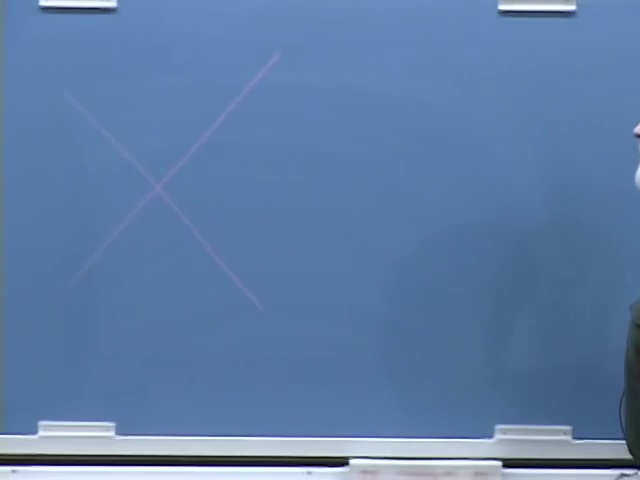
\includegraphics[width=0.68\textwidth]{lecture_09_figure_02.png}
\caption{Die Hawking-Temperatur \(T_H=1/(8\pi M)\) in natürlichen Einheiten.}
\lectureframe{00:08:12}
\end{figure}

Ein größeres Schwarzes Loch ist kälter. Die Vorlesung erklärt dies, indem sie ein typisches Photon rückwärts verfolgt. Thermische Photonen haben eine charakteristische Energie \(E_\gamma\sim T_H\). Ein Photon, das das Unendliche mit einer Energie in der Größenordnung von \(M^{-1}\) erreicht, hatte nahe am Horizont eine viel größere lokale Energie. Bei einem größeren Schwarzen Loch ist die Rotverschiebung zwischen der Schicht nahe dem Horizont und dem Unendlichen stärker; dadurch ist die asymptotische Temperatur niedriger.

\begin{classroomqa}
\audiencequestion{Wenn die Schwarzschild-Zeit am Horizont einfriert, sollten wir dann das Photon verfolgen, das ursprünglich hineingefallen ist und das Schwarze Loch aufgebaut hat?\lecturetimestamp{00:04:19}}
\lecturerresponse{Für die Temperaturfrage verfolgen wir die nach außen emittierten Photonen. Sie beginnen mit sehr hoher lokaler Frequenz, verlieren beim Aufsteigen Energie und treffen als Hawking-Strahlung ein. Was mit dem ursprünglich hineingefallenen Photon geschieht, ist eine gesonderte Frage der Information.}
\end{classroomqa}

\section{Die Planck-Schicht und der gestreckte Horizont}

Wie nahe am Horizont gilt die lokale Beziehung in Gleichung~\eqref{eq:l09-local-temperature}? Die Vorlesung setzt die Planck-Länge als den kleinsten sinnvollen Abstand in der semiklassischen Beschreibung an. Das legt eine dünne Schicht nahe, ungefähr eine Planck-Länge außerhalb des mathematischen Horizonts, die von Fluktuationen auf der Planck-Skala erfüllt ist. Sie emittiert und absorbiert fortwährend.

Die meisten emittierten Quanten entkommen nicht. Nur diejenigen, die in einen sehr schmalen Kegel nach außen gerichtet sind, entgehen dem Zurückfallen. Quanten, die unter allgemeinen Winkeln ausgesandt werden, kehren zum Horizont zurück. Auslaufende und einlaufende Anregungen stoßen zusammen und erzeugen Paare und andere Teilchen; in diesem Sinne enthält die stationäre Beschreibung eine dünne Schale extrem heißer Materie.

\begin{figure}[htbp]
\centering
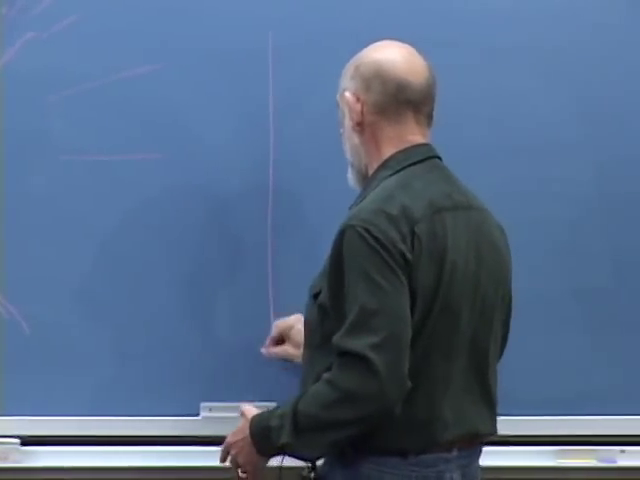
\includegraphics[width=0.74\textwidth]{lecture_09_figure_03.png}
\caption{Der schmale Entweichungskegel für Strahlung nahe dem Horizont. Die meisten lokal emittierten Quanten kehren zum Horizont zurück.}
\lectureframe{00:11:38}
\end{figure}

Es gibt ein ergänzendes raumzeitliches Bild. Weit entfernt von einem Horizont lässt sich eine virtuelle Fluktuation schematisch als kurze geschlossene Schleife darstellen: Eine Teilchen-Antiteilchen-Anregung entsteht und verschwindet, bevor sie zu einem asymptotischen Zustand werden kann. Nahe einem Horizont kann eine Fluktuation die Kausalgrenze übergreifen. Für den äußeren Beobachter sieht der außerhalb liegende Teil wie ein vom Horizont emittiertes und später wieder absorbiertes Teilchen aus. Ein sehr kleiner Anteil entkommt und wird zu Hawking-Strahlung.

\begin{classroomqa}
\audiencequestion{Erstreckt sich eine solche Fluktuation im Außengebietsdiagramm von \(t=-\infty\) bis \(t=+\infty\)?\lecturetimestamp{00:15:00}}
\lecturerresponse{Der exakte klassische Horizont führt zu dieser singulär anmutenden Beschreibung. In der Praxis ersetzen wir ihn durch einen gestreckten Horizont, eine zeitartige Fläche etwa eine Planck-Länge außerhalb. Emission und Reabsorption finden dann zu endlichen äußeren Zeiten statt.}
\end{classroomqa}

\begin{figure}[htbp]
\centering
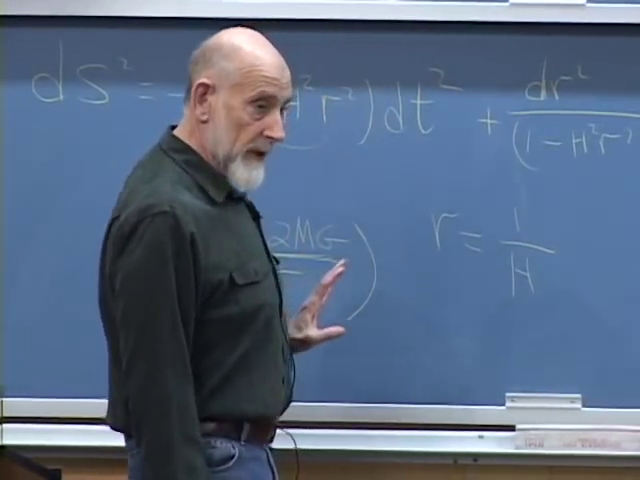
\includegraphics[width=0.72\textwidth]{lecture_09_figure_04.png}
\caption{Der klassische Horizont und der nahe gelegene gestreckte Horizont, der in der Beschreibung des Außengebiets verwendet wird.}
\lectureframe{00:15:52}
\end{figure}

Der gestreckte Horizont ist keine neue invariante Grenze. Er ist eine effektive Fläche an der Stelle, an der die semiklassische Geometrie ihre Zuverlässigkeit verliert. Quantenfluktuationen der Materie und der Geometrie selbst verwischen die genaue Lage auf Planck-Skalen. Diese Konstruktion fasst jene Unschärfe in einer Fläche zusammen, auf der die Beschreibung des Außengebiets endlich bleibt.

Nichts in dieser lokalen Argumentation verrät, ob der Horizont zu einem Schwarzen Loch oder zu einem beschleunigt expandierenden Universum gehört. Das ist die Brücke zum de-Sitter-Raum.

\section{Der de-Sitter-Raum in expandierenden Koordinaten}

Die formale Vorlesung beginnt mit der räumlich flachen Schichtung der de-Sitter-Raumzeit:
\begin{equation}
ds^2=-dt^2+e^{2Ht}d\mathbf{x}^2,
\qquad
d\mathbf{x}^2=dx^2+dy^2+dz^2.
\label{eq:l09-flat-slicing}
\end{equation}
Die Konstante \(H\) ist die Expansionsrate des de-Sitter-Raums. Der Faktor tritt als \(e^{2Ht}\) auf, weil die Metrik das Abstandsquadrat misst; ein festes Koordinatenintervall hat die physikalische Länge
\begin{equation}
D(t)=e^{Ht}\lvert\Delta\mathbf{x}\rvert.
\end{equation}

\begin{figure}[htbp]
\centering
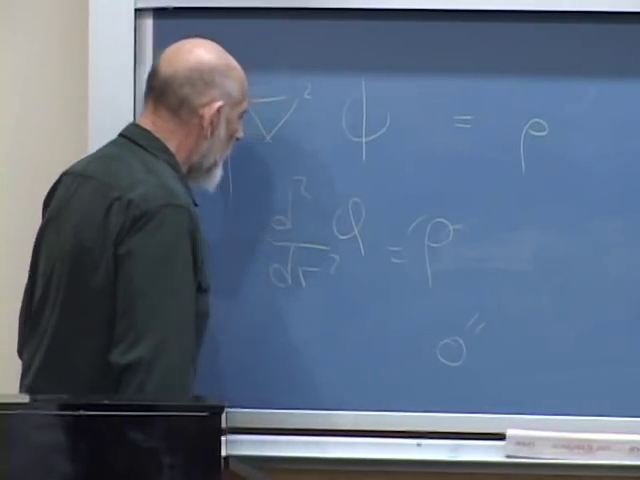
\includegraphics[width=0.78\textwidth]{lecture_09_figure_05.png}
\caption{Die exponentiell expandierende de-Sitter-Metrik in flachen Koordinaten.}
\lectureframe{00:18:50}
\end{figure}

Diese Koordinaten machen die Expansion anschaulich, legen aber die zukünftige Unendlichkeit unendlich weit oben auf der Seite. Um sie auf die Tafel zu holen, führen wir die konforme Zeit ein:
\begin{equation}
\eta=-\frac{1}{H}e^{-Ht},
\qquad
-\infty<\eta<0.
\label{eq:l09-conformal-time}
\end{equation}
Dann gilt
\begin{equation}
dt=\frac{d\eta}{-H\eta},
\qquad
e^{Ht}=-\frac{1}{H\eta},
\end{equation}
und Gleichung~\eqref{eq:l09-flat-slicing} wird zu
\begin{equation}
ds^2=\frac{1}{H^2\eta^2}
\left(-d\eta^2+d\mathbf{x}^2\right).
\label{eq:l09-conformal-metric}
\end{equation}
Für \(t\to+\infty\) gilt \(\eta\to0^{-}\). Die unendliche Eigenzeit wird auf die endliche horizontale Linie \(\eta=0\) abgebildet.

\editorialnote{Die Zeittransformation wird beim Anschreiben an der Tafel mehrfach korrigiert. Gleichung~\eqref{eq:l09-conformal-time} ist die konsistente Form: Frühe kosmische Zeiten entsprechen \(\eta\to-\infty\), und die zukünftige Unendlichkeit entspricht \(\eta\to0^{-}\).}

\begin{figure}[htbp]
\centering
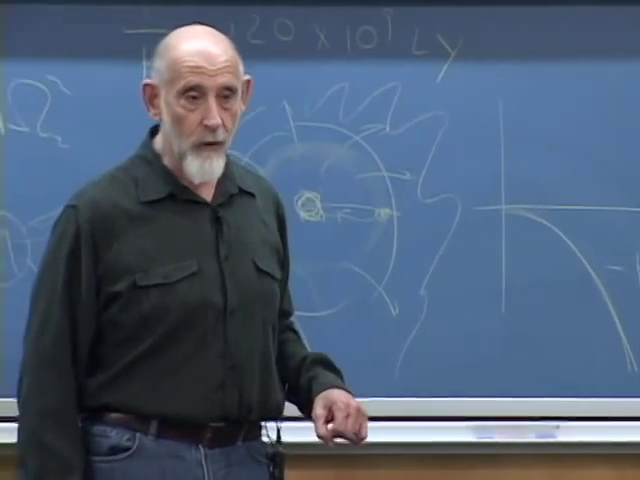
\includegraphics[width=0.82\textwidth]{lecture_09_figure_06.png}
\caption{Die Transformation zur konformen Zeit und die konform flache Metrik.}
\lectureframe{00:21:24}
\end{figure}

Der konforme Faktor multipliziert sowohl den Zeit- als auch den Raumterm und verändert daher die Nullrichtungen nicht. Für einen radialen Lichtstrahl gilt
\begin{equation}
ds^2=0
\quad\Longrightarrow\quad
-d\eta^2+dx^2=0
\quad\Longrightarrow\quad
\frac{dx}{d\eta}=\pm1.
\label{eq:l09-null-rays}
\end{equation}
Im konformen Diagramm bewegt sich Licht daher unter \(45^\circ\). Deshalb ist diese Koordinatentransformation nützlich: Die kausale Erreichbarkeit wird sichtbar.

\section{Der Kausalbereich eines einzelnen Beobachters}

Man stelle sich einen Beobachter vor, dessen Weltlinie unendlich lange fortbesteht. Im kompakten Diagramm endet sie in einem Punkt auf \(\eta=0\). Jedes Signal, das der Beobachter jemals empfangen kann, liegt innerhalb des rückwärts gerichteten Lichtkegels dieses Endpunkts. Ereignisse außerhalb des Kegels können mit dem Beobachter niemals in Verbindung treten, wie lange er auch wartet.

\begin{figure}[htbp]
\centering
\includegraphics[width=0.78\textwidth]{lecture_09_figure_07.png}
\caption{Der rückwärts gerichtete Grenzlichtkegel eines Beobachters in konformen de-Sitter-Koordinaten.}
\lectureframe{00:24:38}
\end{figure}

Ein zweiter Beobachter hat einen anderen Kegel. Die beiden zugänglichen Gebiete überlappen sich, aber keines von ihnen umfasst die gesamte Raumzeit. Für den Rest der Argumentation nehmen wir den Standpunkt des ersten Beobachters ein und nennen diesen rückwärts gerichteten Lichtkegel den Kausalbereich des Beobachters.

Die Zeichnung scheint zu zeigen, wie der Kausalbereich in Richtung Zukunft schrumpft, doch die Koordinatenbreite ist kein Eigenabstand. Auf einer Fläche konstanter \(\eta\) beträgt das Quadrat des physikalischen Abstands zwischen dem Beobachter bei \(x=0\) und dem Horizont bei \(x=\Delta x\)
\begin{equation}
D^2=\frac{(\Delta x)^2}{H^2\eta^2}.
\label{eq:l09-horizon-distance-start}
\end{equation}
Der Horizont ist eine \(45^\circ\)-Nullgerade, die bei \(\eta=0\) endet, also gilt
\begin{equation}
\Delta x=\lvert\eta\rvert.
\end{equation}
Einsetzen ergibt
\begin{equation}
D_{\rm hor}^2=\frac{1}{H^2},
\qquad
D_{\rm hor}=\frac{1}{H}.
\label{eq:l09-horizon-radius}
\end{equation}
Der Koordinatenabstand schrumpft, aber der konforme Faktor wächst genau um den kompensierenden Betrag. Der Eigenradius des Horizonts ist konstant.

\begin{figure}[htbp]
\centering
\includegraphics[width=0.80\textwidth]{lecture_09_figure_08.png}
\caption{Die Herleitung an der Tafel, die das schrumpfende Koordinatenintervall in den festen Eigenabstand \(H^{-1}\) umwandelt.}
\lectureframe{00:28:42}
\end{figure}

\section{Das statische Beobachtergebiet}

Ein fester Horizontsradius legt Koordinaten nahe, die an den zentralen Beobachter angepasst sind. Ohne die Koordinatentransformation herzuleiten, schreibt die Vorlesung das Ergebnis an:
\begin{equation}
ds^2=
-\left(1-H^2r^2\right)d\tau^2
+\frac{dr^2}{1-H^2r^2}
+r^2d\Omega_2^2.
\label{eq:l09-static-patch}
\end{equation}
Die Koeffizienten hängen von \(r\) ab, nicht von \(\tau\). Diese Karte überdeckt das statische Beobachtergebiet,
\begin{equation}
0\le r<\frac{1}{H}.
\end{equation}

\begin{figure}[htbp]
\centering
\includegraphics[width=0.88\textwidth]{lecture_09_figure_09.png}
\caption{Die Metrik des statischen de-Sitter-Beobachtergebiets und ihr Vergleich mit dem Schwarzschild-Faktor.}
\lectureframe{00:34:22}
\end{figure}

Die Ähnlichkeit mit der Schwarzschild-Geometrie ist unmittelbar erkennbar:
\begin{equation}
f_{\rm dS}(r)=1-H^2r^2,
\qquad
f_{\rm Schw}(r)=1-\frac{2G_NM}{r}.
\end{equation}
In beiden Fällen liegt der Horizont der statischen Koordinaten dort, wo \(f(r)=0\) gilt. Für den de-Sitter-Raum gilt
\begin{equation}
1-H^2r^2=0
\quad\Longrightarrow\quad
r_H=H^{-1}.
\end{equation}
Die Karte ist dort singulär, ebenso wie die Schwarzschild-Koordinaten am Horizont eines Schwarzen Lochs singulär sind. Die globalen Geometrien unterscheiden sich dennoch in einem wichtigen Punkt. Ein Beobachter bei einem Schwarzen Loch steht außen und blickt nach innen; ein de-Sitter-Beobachter steht innen und blickt nach außen.

\begin{classroomqa}
\audiencequestion{Wie kann die Geometrie statisch sein, wenn frei gelassene Teilchen sich in einem exponentiell expandierenden Universum voneinander entfernen?\lecturetimestamp{00:36:06}}
\lecturerresponse{Statisch bedeutet nicht, dass jedes Teilchen an seinem Ort bleibt. Es bedeutet, dass die Metrikkoeffizienten und das Ergebnis eines wiederholten Experiments unabhängig vom Startzeitpunkt sind. Lässt man zwei Teilchen jetzt frei, beschleunigen sie voneinander weg; wiederholt man dasselbe Experiment später, geschieht dieselbe Bewegung.}
\end{classroomqa}

\begin{classroomqa}
\audiencequestion{Sehen die beiden auseinanderdriftenden Teilchen einander rotverschoben?\lecturetimestamp{00:38:34}}
\lecturerresponse{Ja. Ihr zunehmender Abstand führt zu einer relativen Rotverschiebung, obwohl die an den Beobachter angepasste Metrik zeitunabhängig ist.}
\end{classroomqa}

\section{Temperaturmessung von innen}

Die Strukturen nahe dem Horizont sind im Schwarzschild- und im de-Sitter-Raum lokal äquivalent. Daher emittiert und reabsorbiert auch der de-Sitter-Horizont thermische Quanten. Ein seltenes Photon bewegt sich nach innen zum zentralen Beobachter und verliert Energie, während es das Potential des statischen Beobachtergebiets hinaufsteigt. Die im Zentrum gemessene Gibbons---Hawking-Temperatur beträgt
\begin{equation}
T_{\rm dS}=\frac{H}{2\pi}
\label{eq:l09-de-sitter-temperature}
\end{equation}
in natürlichen Einheiten. Ein stationäres Thermometer bei Radius \(r\) zeigt den nach Tolman rotverschobenen Wert
\begin{equation}
T_{\rm local}(r)=
\frac{T_{\rm dS}}{\sqrt{1-H^2r^2}},
\label{eq:l09-tolman}
\end{equation}
an, der für \(r\to H^{-1}\) divergiert und nahe dem Horizont auf Gleichung~\eqref{eq:l09-local-temperature} zurückgeht.

\editorialnote{Die Vorlesung gewinnt die Größenordnung aus dem Horizontabstand und der Rotverschiebung, statt die Gleichungen~\eqref{eq:l09-de-sitter-temperature} und \eqref{eq:l09-tolman} ausdrücklich anzuschreiben. Sie geben die Standardnormierung dieser Argumentation an.}

Für die beobachtete Beschleunigung in der späten kosmischen Epoche verwendet die Vorlesung die Abschätzung für den Zeitraum
\begin{equation}
H^{-1}\sim 20\times10^9\ {\rm light\ years}.
\label{eq:l09-lecture-horizon-estimate}
\end{equation}
Ein typisches Horizontphoton hat dann eine Wellenlänge, die mit mehreren Milliarden Lichtjahren vergleichbar ist. Es handelt sich nicht um Mikrowellenhintergrundstrahlung; sie ist um vieles kälter.

Das operative Gedankenexperiment verwendet eine Angelrute im kosmologischen Maßstab. Alice bleibt bei \(r=0\), befestigt ein Thermometer an einer sehr langen Schnur, die zugleich Daten überträgt, und lässt die kosmische Abstoßung das Instrument nach außen tragen. Sie hält es knapp vor dem Horizont an, wartet auf die Rückkehr des Signals und stellt eine hohe lokale Temperatur fest. Das Thermometer neben ihr im Zentrum zeigt den kleinen Wert \(H/(2\pi)\) an. Derselbe Horizont ermöglicht beide Messwerte, weil sie bei unterschiedlichen Gravitationspotentialen gewonnen werden.

\section{Den Horizont überqueren}

Die klassische Beschreibung von außen ähnelt der bekannten Geschichte über Schwarze Löcher. Bob im Zentrum beobachtet, wie Alice sich entfernt. Ihre Signale werden zunehmend rotverschoben und treffen in immer größeren zeitlichen Abständen ein; sie scheint sich am Horizont abzuflachen und verblasst schließlich. Eine spätere Reisende, Jane, erscheint als eine weitere, dünnere Schicht in einem sedimentartigen Stapel nahe der Grenze.

\begin{classroomqa}
\audiencequestion{Überqueren Objekte aus unserer Sicht jemals den kosmischen Horizont?\lecturetimestamp{00:45:30}}
\lecturerresponse{In der klassischen Beschreibung des statischen Beobachters nicht. Ihre Signale werden rotverschoben und verblassen, während ihre scheinbare Position sich dem Horizont nähert. In ihrer eigenen frei fallenden Beschreibung überqueren sie ihn jedoch, ohne auf eine lokal singuläre Fläche zu treffen.}
\end{classroomqa}

\begin{classroomqa}
\audiencequestion{Ist der Horizont nur für Beobachter heiß, die in seiner Nähe bleiben, ohne ihn zu überqueren? Wird eine hineinfallende Beobachterin beim Durchgang nicht einfach gebraten?\lecturetimestamp{00:48:27}}
\lecturerresponse{Alice überquert ihn in ihrem eigenen Bezugssystem ungestört. Die extreme Temperatur gehört zur stationären Beschreibung. Wenn Bob darauf besteht, Alice immer näher am Horizont aufzulösen, muss er sie mit immer kürzeren Wellenlängen beleuchten. Das gedachte Heisenberg-Mikroskop deponiert dann so viel Energie, dass es das Objekt, das es beobachten soll, brät.}
\end{classroomqa}

Dies ist kein Widerspruch zwischen zwei lokalen Ereignissen. Der stationäre Beobachter und die hineinfallende Beobachterin verwenden grundverschiedene Messverfahren. Die Horizontkomplementarität fragt, wie beide Beschreibungen gültig sein können, ohne dass ein Beobachter direkt doppelte Information vergleichen kann.

\section{Ein Newtonsches Modell der Vakuumabstoßung}

An dieser Stelle fragt ein Student, was im de-Sitter-Raum an die Stelle des Gravitationspotentials eines Schwarzen Lochs tritt. Susskind entwickelt dazu ein Newtonsches Modell. Sei \(\phi\) das Gravitationspotential; dann ist die Beschleunigung eines Testteilchens
\begin{equation}
\mathbf{a}=-\boldsymbol{\nabla}\phi.
\end{equation}
Für gewöhnliche nichtrelativistische Materie lautet die Poisson-Gleichung
\begin{equation}
\nabla^2\phi=4\pi G_N\rho.
\label{eq:l09-poisson}
\end{equation}

\begin{classroomqa}
\audiencequestion{Wenn die Effekte des Schwarzen Lochs von seinem Gravitationspotential herrühren, was ist dann die entsprechende Quelle im de-Sitter-Raum?\lecturetimestamp{00:49:36}}
\lecturerresponse{Die Vakuumenergie selbst liefert eine räumlich homogene Gravitationsquelle. In einer Newtonschen Beschreibung erzeugt sie ein quadratisches Potential statt eines \(1/r\)-Potentials.}
\end{classroomqa}

\begin{figure}[htbp]
\centering
\includegraphics[width=0.78\textwidth]{lecture_09_figure_10.png}
\caption{Die Poisson-Gleichung und die schematische radiale Form mit der zweiten Ableitung aus der Vorlesung.}
\lectureframe{00:51:38}
\end{figure}

An der Tafel werden Normierung, Terme aus dem Kugelmaß, der Druck und zunächst sogar das Vorzeichen weggelassen; die Aufgabe wird so reduziert auf
\begin{equation}
\frac{d^2\phi}{dr^2}\sim H^2.
\end{equation}
Die wesentliche Folgerung ist, dass eine konstante Quelle eine quadratische Funktion ergibt. Mit dem für die Abstoßung im de-Sitter-Raum erforderlichen Vorzeichen gilt
\begin{equation}
\phi_{\rm dS}(r)=-\frac{1}{2}H^2r^2,
\qquad
a_r=-\frac{d\phi_{\rm dS}}{dr}=H^2r.
\label{eq:l09-de-sitter-potential}
\end{equation}
Die Beschleunigung zeigt nach außen und wächst linear mit dem Abstand. Die Lösung von \(\ddot r=H^2r\) lautet
\begin{equation}
r(\tau)=A e^{H\tau}+B e^{-H\tau},
\end{equation}
Der wachsende Lösungszweig ergibt somit erneut eine exponentielle Trennung.

\begin{figure}[htbp]
\centering
\includegraphics[width=0.76\textwidth]{lecture_09_figure_11.png}
\caption{Die Gleichung mit homogener Quelle und das quadratische de-Sitter-Potential.}
\lectureframe{00:53:32}
\end{figure}

\editorialnote{In der allgemeinen Relativitätstheorie hängt die Beschleunigung im Schwachfeld einer homogenen Flüssigkeit von \(\rho+3p\) ab und nicht allein von \(\rho\). Für Vakuumenergie gilt \(p=-\rho\), also ist \(\rho+3p=-2\rho\) und die Beschleunigung wirkt abstoßend. Gleichung~\eqref{eq:l09-de-sitter-potential} ist das korrekt normierte de-Sitter-Ergebnis; in der Rechnung an der Tafel werden bewusst nur der quadratische Zusammenhang und das Vorzeichen betrachtet.}

Man platziere eine gewöhnliche Masse \(M\) im Zentrum. Das qualitative Potential lautet dann
\begin{equation}
\phi(r)=-\frac{G_NM}{r}-\frac{1}{2}H^2r^2,
\label{eq:l09-combined-potential}
\end{equation}
und die radiale Beschleunigung
\begin{equation}
a_r=-\frac{G_NM}{r^2}+H^2r.
\end{equation}
Bei kleinem \(r\) überwiegt die lokale Anziehung; bei großem \(r\) die Vakuumabstoßung. Ihr Gleichgewicht liegt bei
\begin{equation}
r_\ast=\left(\frac{G_NM}{H^2}\right)^{1/3}.
\label{eq:l09-turnaround}
\end{equation}
Dies ist die saubere Fassung des Potenzialmaximums aus der Vorlesung. Sie erklärt qualitativ, warum nahe gelegene, gravitativ gebundene Systeme zusammenbleiben können, während ausreichend weit entfernte Galaxien beschleunigt auseinanderdriften.

\begin{figure}[htbp]
\centering
\includegraphics[width=0.78\textwidth]{lecture_09_figure_12.png}
\caption{Anziehung durch gewöhnliche \(1/r\)-Kraft zusammen mit dem umgekehrt gekrümmten quadratischen de-Sitter-Potential.}
\lectureframe{00:58:20}
\end{figure}

\begin{classroomqa}
\audiencequestion{Spielen gewöhnliche Kräfte weiterhin eine Rolle, oder zerreißt die Vakuumrepulsion schließlich jede Insel aus Materie?\lecturetimestamp{00:57:29}}
\lecturerresponse{Alle Kräfte müssen berücksichtigt werden. Auf hinreichend kleinen Skalen dominieren die elektromagnetische Bindung und die lokale Gravitation. Vakuumrepulsion wird erst über gewaltige Entfernungen wichtig, die durch \(H^{-1}\) und die für die gebundene Masse maßgebliche Gleichgewichtsskala bestimmt sind.}
\end{classroomqa}

\section{Eine Quelle, mehrere Bezeichnungen}

Nun hält die Diskussion inne, um die Begriffe zu klären. Vakuumenergie, kosmologische Konstante und dunkle Energie sind in dem verwendeten Modell keine drei additiven Substanzen. Sie bezeichnen ein und dieselbe Quelle mit Zustandsgleichung \(w=-1\). Man kann von einem konstanten Term in der Einsteinschen Gleichung, einer Lorentz-invarianten Energiedichte des Vakuums oder der Komponente sprechen, die die späte kosmische Beschleunigung antreibt.

\begin{classroomqa}
\audiencequestion{Treten die homogene Newtonsche Quelle und die quantenmechanische Vakuumenergie als getrennte Effekte zugleich auf?\lecturetimestamp{00:59:14}}
\lecturerresponse{Nein. Die homogene Dichte ist das Newtonsche Modell derselben Quelle. Vakuumenergie, kosmologische Konstante und in dieser Vorlesung dunkle Energie bezeichnen eine einzige physikalische Komponente.}
\end{classroomqa}

\begin{classroomqa}
\audiencequestion{Hat dasselbe Phänomen demnach sowohl eine klassische als auch eine quantenmechanische Beschreibung?\lecturetimestamp{01:00:32}}
\lecturerresponse{Sein mikroskopischer Ursprung kann quantenmechanisch sein, so wie auch ein Teil der Masse eines Elektrons einen quantenmechanischen Ursprung hat. Sobald die effektive Energiedichte bekannt ist, geht sie als gewöhnliche Quelle in die klassischen Gravitationsgleichungen ein. Den letztlichen Ursprung des beobachteten Werts kennen wir nicht.}
\end{classroomqa}

In Planck-Einheiten ist die beobachtete Vakuumenergiedichte außerordentlich klein:
\begin{equation}
\rho_\Lambda\sim10^{-123}\rho_{\rm Pl},
\label{eq:l09-planck-smallness}
\end{equation}
bis auf die verwendete Konvention für die Planck-Dichte. Diese kleine Zahl ist der Kern des Problems der kosmologischen Konstante. Sie erklärt auch, warum der Horizont so groß ist: In vier Dimensionen gilt
\begin{equation}
H^2=\frac{8\pi G_N}{3}\rho_\Lambda,
\qquad
r_H=H^{-1}.
\end{equation}
Wäre \(H\) größer, wäre der Horizont kleiner, die zentrale de-Sitter-Temperatur höher und die abstoßende Beschleunigung \(H^2r\) stärker.

\begin{classroomqa}
\audiencequestion{Hängt die winzige kosmologische Konstante mit dem Planckschen Wirkungsquantum und Quantenfluktuationen zusammen?\lecturetimestamp{01:03:27}}
\lecturerresponse{Ein sauberer Vergleich verwendet dimensionslose Planck-Einheiten, in denen \(G_N=\hbar=c=1\) gilt. In diesen Einheiten liegt die Vakuumdichte etwa \(123\) Größenordnungen unter der natürlichen Planck-Dichte. Diese Hierarchie zu erklären, gehört zu den zentralen Rätseln der Grundlagenphysik.}
\end{classroomqa}

\begin{classroomqa}
\audiencequestion{Muss die Vakuumenergie eine exakt konstante kosmologische Konstante sein? Könnte die beschleunigende Komponente abnehmen und schließlich gegen null gehen?\lecturetimestamp{01:04:52}}
\lecturerresponse{Das ist eine logisch mögliche Alternative: Ein dynamisches Dunkle-Energie-Feld könnte sich mit der Zeit ändern. Die Vorlesung nimmt den konstanten Fall an, weil die damals verfügbaren Beobachtungen zunehmend ein Verhalten nahe an dem einer kosmologischen Konstante nahelegten, nicht weil jede Alternative als unmöglich bewiesen worden wäre.}
\end{classroomqa}

\section{Astronomie in ferner Zukunft}

In einem asymptotisch de-Sitter-artigen Universum überschreiten Strukturen, die nicht gravitativ gebunden sind, irgendwann den Horizont des Beobachters. Die kosmische Mikrowellenhintergrundstrahlung verschiebt sich unter die Nachweisgrenze. Entfernte Galaxien verschwinden. Ein überlebender Astronom könnte dann nur noch eine verschmolzene lokale Gravitationsinsel in einem ansonsten dunklen Kausalbereich sehen.

\begin{classroomqa}
\audiencequestion{Würde überhaupt jemand ohne Teleskop bemerken, dass die fernen Galaxien verschwunden sind?\lecturetimestamp{01:06:17}}
\lecturerresponse{Wahrscheinlich nicht. Das eigentliche Problem liegt tiefer: Selbst mit fortgeschrittenen Instrumenten könnten künftigen Beobachtern die fernen Anhaltspunkte und die Mikrowellenhintergrundstrahlung fehlen, aus denen wir heute auf die Expansion schließen.}
\end{classroomqa}

Dann könnte das alte Bild der Inseluniversen überzeugend wirken. Olbers' Paradoxon würde keine andere Schlussfolgerung erzwingen, denn es setzt eine unendliche, statische und gleichförmige Population leuchtender Quellen voraus; der zukünftige Beobachter sähe nur die endlichen Sterne der lokalen Insel. Dunkle Energie erzeugt nicht fortwährend Ersatzgalaxien aus dem leeren Raum.

Im exakten de-Sitter-Raum schrumpft der Horizont nicht um die lokale Galaxie. Sein physikalischer Radius bleibt \(H^{-1}\) und ist sehr viel größer als eine Galaxie. Was verschwindet, ist die ungebundene Materie, die über diese feste Kausalgrenze hinausgetragen wird.

\begin{classroomqa}
\audiencequestion{Könnten aus der Galaxie herausgeschleuderte Sterne als Testkörper dienen, um die großräumige Geometrie nachzuweisen?\lecturetimestamp{01:11:25}}
\lecturerresponse{Eine Zeit lang, ja. Ausgeschleuderte Objekte und Lichtsignale über große Basislinien könnten die Geometrie untersuchen. Der Effekt wird aber erst über Entfernungen merklich, die einen beträchtlichen Bruchteil einer Milliarde Lichtjahre ausmachen; das Experiment würde also kosmische Zeiträume erfordern.}
\end{classroomqa}

\begin{classroomqa}
\audiencequestion{Woher wissen wir, dass ein ferner Horizont nicht bereits den größten Teil des Universums vor uns verborgen hat?\lecturetimestamp{01:11:45}}
\lecturerresponse{Wir sehen bereits genug Galaxien, Rotverschiebungen und Hintergrundstrahlung, um die Expansion zu messen und die großräumige Geometrie zu rekonstruieren. Künftige Beobachter, denen diese Anhaltspunkte fehlen, stünden vor einer wesentlich schwierigeren Schlussfolgerung.}
\end{classroomqa}

\begin{classroomqa}
\audiencequestion{Wäre es offensichtlich, wenn der Horizont gerade jenseits von Andromeda läge?\lecturetimestamp{01:12:19}}
\lecturerresponse{Ja. Ein derart kleiner Horizont würde ein viel größeres \(H\) erfordern, und die daraus folgende Abstoßung würde die Bewegung Andromedas stark verändern. Der gemessene Wert verortet den asymptotischen Horizont dagegen auf einer ungleich größeren Skala.}
\end{classroomqa}

\begin{classroomqa}
\audiencequestion{Könnten sich jenseits unseres Horizonts neue Urknalle ereignen?\lecturetimestamp{01:13:25}}
\lecturerresponse{Ereignisse jenseits des Horizonts sind weder für uns noch für unsere Nachkommen sichtbar. Eine verwandte, aber genauere Möglichkeit, die Blasenkeimbildung in ewiger Inflation, wird später in der Vorlesung eingeführt.}
\end{classroomqa}

Mit Raketen, Uhren und mehreren Milliarden Jahren könnten zukünftige Beobachter Forschungsreisende über einen großen Teil des Kausalbereichs schicken und seine Metrik rekonstruieren. Auf gewöhnlichen Labor- oder Zivilisationszeitskalen ist der Effekt jedoch nahezu unzugänglich. Diese Unterscheidung korrigiert die allzu starke Behauptung, die Expansion wäre unmöglich zu entdecken: Sie ist praktisch fern, aber nicht prinzipiell ausgeschlossen.

\begin{classroomqa}
\audiencequestion{Könnten zukünftige Forschungsreisende die Geometrie viel früher bestimmen, als auf eine thermische Wiederkehr zu warten?\lecturetimestamp{01:21:40}}
\lecturerresponse{Natürlich. Eine Wiederkehr ist nicht die vorgeschlagene Messmethode. Forschungsreisende, die über Basislinien von Milliarden Lichtjahren Lichtsignale austauschen, könnten das statische Beobachtergebiet auf einer wesentlich kürzeren, wenn auch immer noch kosmischen Zeitskala kartieren.}
\end{classroomqa}

\begin{classroomqa}
\audiencequestion{Würde die Rotverschiebung alle Informationen auslöschen, die solche Forscher zurücksenden?\lecturetimestamp{01:23:24}}
\lecturerresponse{Nicht, wenn sie Skalen weit innerhalb des Horizonts untersuchen. Eine Basislinie in der Größenordnung von einer Milliarde Lichtjahren ist bereits empfindlich für die Expansion und erzeugt dabei nur eine moderate Rotverschiebung. Das Experiment wird vor allem durch seine enorme Dauer begrenzt.}
\end{classroomqa}

\section{Endliche Entropie und Wiederkehr}

Der statische Patch ist im thermodynamischen Sinn nicht leer. Sein Horizont hat die Fläche
\begin{equation}
A_H=4\pi H^{-2},
\end{equation}
und die Temperatur \(T_{\rm dS}=H/(2\pi)\) sowie die Entropie
\begin{equation}
S_{\rm dS}=\frac{A_H}{4G_N}
=\frac{\pi}{G_NH^2}
\label{eq:l09-de-sitter-entropy}
\end{equation}
in den Einheiten \(\hbar=c=k_B=1\). Die Entropie ist endlich. Daher kann man sich den statischen Patch mit der gebotenen Vorsicht als thermischen Hohlraum endlicher Entropie vorstellen, dessen Anregungen in der stationären Beschreibung nahe am Horizont konzentriert sind.

Ein gewöhnlicher Gaskasten im Gleichgewicht erscheint auf kurzen Zeitskalen strukturlos, doch die statistische Mechanik verbietet Fluktuationen nicht. Hat ein Makrozustand gegenüber dem Gleichgewicht ein Entropiedefizit \(\Delta S\), so ist seine Wahrscheinlichkeit ungefähr
\begin{equation}
P\sim e^{-\Delta S}.
\label{eq:l09-fluctuation-probability}
\end{equation}
Die zugehörige Wartezeit wächst wie
\begin{equation}
t\sim t_0 e^{\Delta S}.
\end{equation}
Für ein endliches System ist die Zeit, nach der ein Zustand beliebig nahe an einen früheren Zustand zurückkehrt, die Poincaré-Wiederkehrzeit,
\begin{equation}
t_{\rm rec}\sim H^{-1}e^{S_{\rm dS}}.
\label{eq:l09-recurrence}
\end{equation}
Da \(S_{\rm dS}\) für unseren Horizont in der Größenordnung von \(10^{120}\) liegt, fasst die Vorlesung die Skala als \(e^{10^{120}}\) zusammen. Ob der Vorfaktor in Jahren, Hubble-Zeiten oder mikroskopischen Einheiten gemessen wird, ist neben der doppelten Exponentialfunktion unerheblich.

\begin{figure}[htbp]
\centering
\includegraphics[width=0.76\textwidth]{lecture_09_figure_13.png}
\caption{Die Diskussion der Wiederkehr mit der enormen exponentiellen Wartezeitskala an der Tafel.}
\lectureframe{01:16:24}
\end{figure}

Vor einer solchen Wiederkehr sind kleinere Fluktuationen sehr viel häufiger. Die Moleküle in einem Raum könnten sich alle in einer Ecke sammeln; kurzzeitig könnte sich ein komplizierter Wirbel bilden; in der spielerischen Hierarchie der Vorlesung könnte die Wärmebewegung sogar einen Elefanten zusammenfügen. Je kleiner das erforderliche Entropiedefizit ist, desto geringer sind die Kosten der Fluktuation.

\begin{classroomqa}
\audiencequestion{Sind Poincaré-Wiederkehren eine spezifische Folge der Quantenmechanik?\lecturetimestamp{01:25:44}}
\lecturerresponse{Nein. Wiederkehr und seltene Fluktuationen treten bereits in der klassischen statistischen Mechanik auf. Ihre Anwendung auf den de-Sitter-Raum beruht auf unserem gegenwärtigen physikalischen Rahmen, der eines Tages überarbeitet werden könnte; Thermodynamik und statistisches Denken gehören jedoch zu den robustesten Strukturen, die wir kennen.}
\end{classroomqa}

Die Bedeutung der Wahrscheinlichkeit selbst könnte sich in einer künftigen Theorie vertiefen. Susskind behauptet nicht das Gegenteil. Sein enger gefasster Punkt ist, dass man eines der am besten bestätigten Ordnungsprinzipien der Physik aufgäbe, wenn man die statistische Mechanik nur deshalb verwerfen würde, weil ihre Folgerungen für lange Zeitskalen seltsam sind.

\section{Boltzmann-Gehirne und typische Beobachter}

Angenommen, eine thermische Fluktuation erzeugt einen vollständigen Zustand, der einem Urknall ähnelt. Dafür wäre eine enorme Abnahme der Entropie erforderlich. Eine Fluktuation, die ein einzelnes Sonnensystem hervorbringt, wäre weniger kostspielig; eine bereits warme Erde wäre noch günstiger. Wenn die einzige Voraussetzung ein Beobachter ist, könnte die kostengünstigste Fluktuation lediglich ein funktionsfähiges Gehirn mit scheinbaren Erinnerungen erzeugen. Ein solcher hypothetischer Beobachter wird Boltzmann-Gehirn genannt.

Die Frage ist nicht, ob eine bizarre Fluktuation logisch möglich ist. Es geht darum, ob ein kosmologisches Modell vorhersagt, dass fast jeder Beobachter eine solche Fluktuation ist. Wir schließen aus unseren Beobachtungen, indem wir annehmen, dass wir nicht auf fantastische Weise untypisch sind. Eine Theorie, in der gewöhnliche Beobachter mit kohärenten kosmischen Entwicklungsgeschichten von vereinzelten thermischen Gehirnen exponentiell zahlenmäßig übertroffen werden, untergräbt diesen Schluss.

Das Boltzmann-Gehirn-Problem bezeichnet daher einen quantitativen Konsistenztest. Man vergleicht die erwartete Häufigkeit gewöhnlicher Beobachter mit der Häufigkeit von Beobachtern, die aus Fluktuationen hervorgehen. Überwiegen Letztere, muss entweder das Vakuum zerfallen, bevor sie sich vermehren, das Maß geändert oder die kosmologischen Annahmen neu überdacht werden.

Eine frühere Frage zu einer Verbindung zwischen Ultraviolettbereich--und Infrarotbereich wird ausdrücklich zurückgestellt. Das Wiederkehrargument hängt nicht davon ab, diese separate Frage zu klären.

\section{Ewige Inflation und Blasenuniversen}

Als Nächstes führt die Vorlesung ein zweites Wahrscheinlichkeitsproblem ein, ohne eine vollständige Herleitung zu versuchen. In einem metastabilen de-Sitter-Vakuum kann eine Blase entstehen, in der die Vakuumenergie niedriger ist. Die Blasenwand expandiert, und im Inneren kann sich ein offenes Friedmann--Robertson--Walker-Universum entwickeln. Währenddessen expandiert die umgebende inflierende Region weiter und lässt weitere Blasen entstehen.

\begin{figure}[htbp]
\centering
\includegraphics[width=0.74\textwidth]{lecture_09_figure_14.png}
\caption{Eine Blase mit niedrigerer Vakuumenergie, eingezeichnet innerhalb eines inflierenden de-Sitter-Hintergrunds.}
\lectureframe{01:29:38}
\end{figure}

Das entscheidende Merkmal ist das exponentielle Anwachsen der Population. Es entsteht schneller neues physikalisches Volumen, als Blasen es beseitigen; daher wächst die Zahl der Blasenregionen unbegrenzt. Verschiedene Blasen können sich in unterschiedlichen Niedrigenergiezuständen einrichten und deshalb verschiedene effektive physikalische Gesetze aufweisen.

Um die statistische Schwierigkeit sichtbar zu machen, verlässt Susskind zunächst die Kosmologie und betrachtet eine exponentiell wachsende menschliche Bevölkerung mit begrenzten, aber unbekannten Ressourcen. Man nehme an, dass Beobachter unter allen Menschen, die je leben, typisch sind. Verdoppelt sich die Bevölkerung in jeder Generation und endet dann, lebt die Hälfte aller Menschen in der letzten Generation, drei Viertel leben in den letzten beiden und sieben Achtel in den letzten drei:
\begin{equation}
f_n=1-2^{-n}.
\label{eq:l09-last-generations}
\end{equation}
Nach dem Typikalitätsprinzip wären wir demnach unangenehm nahe am Ende, obwohl wir nichts über den gesamten Ressourcenvorrat wissen. Dies ist keine verlässliche Vorhersage des Aussterbens der Menschheit. Es soll vielmehr davor warnen, dass bei exponentiellem Wachstum die Zählung von der Abschneidegrenze dominiert wird.

Das Beispiel mit dem Münzwurf formuliert die gewöhnliche Typikalitätsannahme klarer. Werfen viele Experimentierende jeweils \(N\)mal eine faire Münze, so erhalten die allermeisten
\begin{equation}
n_H=\frac{N}{2}+O(\sqrt{N}).
\end{equation}
Ein Beobachter mit einem extremen Ergebnis sollte zunächst ein schlechtes Modell oder eine fehlerhafte Münze vermuten, statt ohne Belege anzunehmen, dass er sich in einem extrem seltenen Randbereich befindet. Die kosmologische Wahrscheinlichkeitsbetrachtung folgt demselben Typikalitätsgedanken, braucht aber bei einer unendlichen Population eine wohldefinierte Zählvorschrift.

\section{Eschers Rand und das Maßproblem}

Susskinds geometrische Analogie ist M.\ C.\ Eschers \emph{Circle Limit IV}, die von Engeln und Teufeln gekachelte Scheibe, auf der die Figuren zum Rand hin kleiner erscheinen. In der hyperbolischen Geometrie, die die Zeichnung darstellt, sind die Figuren gleichwertig; ihre scheinbare euklidische Größe ändert sich nur aufgrund der Projektion.

\begin{figure}[htbp]
\centering
\includegraphics[width=0.76\textwidth]{lecture_09_figure_15.png}
\caption{Das Tafelbild als Ersatzdarstellung für Eschers exponentiell anwachsende Figuren nahe einem kreisförmigen Rand.}
\lectureframe{01:37:54}
\end{figure}

Man stelle sich vor, Escher hätte nur begrenzt Zeit, Tinte und Geduld. Am Rand hört er irgendwann auf, vielleicht lässt er einige Figuren unvollendet. Da die Zahl der Figuren mit dem hyperbolischen Radius exponentiell wächst, enthält eine endliche äußere Schicht einen festen Anteil aller gezeichneten Figuren. Etwa die Hälfte kann in der letzten Schicht liegen, ganz gleich, wie weit man die Abschneidegrenze nach außen verschiebt.

Fragt man nun nach dem Verhältnis von Engeln zu Teufeln, legt die Symmetrie des idealen unendlichen Musters ein Verhältnis von eins zu eins nahe. Bei jeder endlichen Zählung kann jedoch eine geringfügig andere Randwahl sehr viel mehr Figuren eines Typs einschließen. Da der größte Teil der gezählten Figuren nahe am Rand liegt, führt eine kleine Verformung dieses Randes zu einer Änderung der Antwort von der Größenordnung eins.

\begin{figure}[htbp]
\centering
\includegraphics[width=0.76\textwidth]{lecture_09_figure_16.png}
\caption{Bei einem exponentiell wachsenden Muster bestimmt die Abschneidegrenze die Zählung maßgeblich.}
\lectureframe{01:43:06}
\end{figure}

Dieselbe Mehrdeutigkeit tritt bei der ewigen Inflation auf. Man zählt blaue und rosa Blasenuniversen unterhalb einer bestimmten Zeitschranke und verschiebt dann die Schranke nach hinten. Beide Anzahlen divergieren, und ihr Verhältnis kann empfindlich davon abhängen, was unter \emph{Zeit} verstanden wird und wie die Abschneidefläche gezogen wird. Ein Wahrscheinlichkeitsmaß ist eine Vorschrift, die die unendliche Population reguliert und relative Wahrscheinlichkeiten ermittelt. Dass verschiedene plausible Vorschriften nicht übereinstimmen, ist das Maßproblem.

\begin{classroomqa}
\audiencequestion{Gibt es einen Zusammenhang zwischen diesem Abschneideproblem und der Renormierung?\lecturetimestamp{01:45:43}}
\lecturerresponse{Es besteht eine Analogie. In der Quantenfeldtheorie führt man ein Gitter oder eine Ultraviolett-Abschneidegrenze ein, verfeinert es beziehungsweise sie und sucht nach Größen, die unempfindlich gegenüber den Einzelheiten am Rand des Regulators sind. Kosmologen hoffen auf eine ebenso robuste Gewinnung von Ergebnissen aus der ewigen Inflation; im hier diskutierten Rahmen gibt es bislang jedoch keine vergleichbar eindeutige Vorschrift.}
\end{classroomqa}

Die Analogie sollte nicht überstrapaziert werden. Die Renormierung ist erfolgreich, wenn ein kontrollierter Fluss regulatorunabhängige Observablen identifiziert. Beim Maßproblem bleiben gerade die entsprechenden invarianten Fragen und das Grenzverfahren unklar. Zu sagen, dass wir vielleicht die falsche Frage stellen, ist keine Lösung, solange die richtige Frage nicht formuliert ist.

\begin{classroomqa}
\audiencequestion{Ist dieses Blasenbild dasselbe Phänomen wie die Inflation im frühen Universum?\lecturetimestamp{01:48:19}}
\lecturerresponse{Es besteht ein enger Zusammenhang. Bei der ewigen Inflation inflatiert der übergeordnete Hintergrund weiter, während sich die Inneren der lokalen Blasen kosmologisch eigenständig entwickeln. Unser beobachtbares Universum könnte sich in einer solchen Region befinden.}
\end{classroomqa}

\section{Kann man Blasenkollisionen beobachten?}

Zwei Blasen addieren ihre Vakuumenergien nicht einfach, wenn sie aufeinandertreffen. Eine Domänenwand trennt Regionen mit unterschiedlichen Vakuumzuständen, und die Geometrie der Wand bestimmt, was auf beiden Seiten beobachtet werden kann. Je nachdem, wo die Kollision relativ zu unserem vergangenen Lichtkegel stattfindet, kann ihr Abdruck verborgen oder sichtbar sein.

\begin{classroomqa}
\audiencequestion{Was geschieht, wenn zwei Vakuumblasen kollidieren?\lecturetimestamp{01:52:07}}
\lecturerresponse{Bei der Kollision entsteht eine Domänenwandgeometrie, deren Verhalten von den beiden Vakuumzuständen und der Wandspannung abhängt. Unter günstigen kausalen Bedingungen kann die Störung in unsere beobachtbare Region gelangen und eine anisotrope Signatur hinterlassen.}
\end{classroomqa}

Die Vorlesung behandelt eine kalte Region in der kosmischen Mikrowellenhintergrundstrahlung als möglichen Kandidaten und verweist auf die Polarisation um ein kreisförmiges Merkmal als Unterscheidungskriterium. Dies wird ausdrücklich als Möglichkeit dargestellt, nicht als Nachweis. Eine überzeugende Signatur einer Kollision wäre revolutionär, denn sie würde direkte Hinweise auf benachbarte Blasenregionen liefern und das Maßproblem experimentell dringlich machen.

\begin{figure}[htbp]
\centering
\includegraphics[width=0.70\textwidth]{lecture_09_figure_17.png}
\caption{Ein kreisförmiges Merkmal am Himmel und sein mögliches Polarisationsmuster in der Diskussion über Blasenkollisionen.}
\lectureframe{01:50:22}
\end{figure}

\editorialnote{Die Diskussion des Kälteflecks hält den Beobachtungsstand und die Vorschläge zum Zeitpunkt der Vorlesung fest. Eine Temperaturanomalie allein ist kein Hinweis auf eine Blasenkollision; erforderlich wäre eine detaillierte, korrelierte Signatur.}

\begin{classroomqa}
\audiencequestion{Sind die Blasen vierdimensional, und welche räumliche Krümmung haben ihre Inneren?\lecturetimestamp{01:53:37}}
\lecturerresponse{Es sind Raumzeitregionen, keine dreidimensionalen Seifenblasen, die sich in einer äußeren Zeit entwickeln. Ihre Inneren sind typischerweise offene FRW-Universen mit negativer räumlicher Krümmung. Eine Kollision verändert diese Geometrie, kehrt aber die negative Krümmung nicht einfach in eine positive um.}
\end{classroomqa}

\section{Was die Stringtheorie begründet und was nicht}

Die abschließende Diskussion beginnt mit der Aufforderung, eine Wahrscheinlichkeit dafür anzugeben, dass die Stringtheorie richtig ist. Susskind lehnt eine Zahl ab, weil die Aussage zu mehrdeutig ist. Stattdessen unterscheidet er zwei Behauptungen.

Erstens gibt es eine stark eingeschränkte mathematische Struktur, die Quantenmechanik und Gravitation vereint. Sie hat präzise Ergebnisse und tiefgehende mathematische Identitäten hervorgebracht, und ihre innere Konsistenz hat eingehender Prüfung standgehalten. In der informellen Ausdrucksweise der Vorlesung ist dies die \emph{Stringtheorie} mit großem \(S\). Die am genauesten verstandenen Versionen stützen sich stark auf Supersymmetrie.

Zweitens ist die beobachtete Welt bei zugänglichen Energien nicht supersymmetrisch. Um die exakten supersymmetrischen Konstruktionen mit unserem nichtsupersymmetrischen Universum zu verbinden, braucht es Supersymmetriebrechung und einen umfassenderen Rahmen, der nicht mit derselben Präzision kontrolliert ist. In der Ausdrucksweise der Vorlesung ist diese erhoffte Erweiterung die \emph{Stringtheorie} mit kleinem \(s\).

\begin{classroomqa}
\audiencequestion{Kann man eine Wahrscheinlichkeit dafür angeben, dass die Stringtheorie die richtige Theorie der Natur ist?\lecturetimestamp{01:54:18}}
\lecturerresponse{Nicht verantwortungsvoll, solange nicht feststeht, welche Behauptung gemeint ist. Die exakten mathematischen Strukturen existieren und umfassen die Quantengravitation, doch die rigoros kontrollierten supersymmetrischen Modelle beschreiben nicht buchstäblich unsere beobachtete Welt. Ob eine umfassendere Erweiterung unsere Welt enthält, ist eine Frage, zu der Physiker begründete Vorannahmen haben können, aber keine wohldefinierte numerische Wahrscheinlichkeit angeben können.}
\end{classroomqa}

Die Analogie ist die Mechanik vor der Entwicklung des vollständigen mathematischen Instrumentariums. Man kennt vielleicht \(F=ma\) und die Kraft mit invers-quadratischem Abstand, kann aber nur hochsymmetrische Kreisbahnen lösen. Dieser lösbare Bereich wäre durchaus echt, aber nicht die ganze Theorie. Ebenso könnten exakte supersymmetrische Stringkonstruktionen einen besonderen, ungewöhnlich gut handhabbaren Bereich einer umfassenderen Struktur darstellen.

\begin{figure}[htbp]
\centering
\includegraphics[width=0.60\textwidth]{lecture_09_figure_18.png}
\caption{Das verschachtelte Bild der Vorlesung: rigoros kontrollierte supersymmetrische Stringkonstruktionen innerhalb eines hypothetisch umfassenderen Rahmens.}
\lectureframe{01:57:34}
\end{figure}

\begin{classroomqa}
\audiencequestion{Warum bricht man die Supersymmetrie nicht einfach in der exakten Theorie?\lecturetimestamp{01:57:02}}
\lecturerresponse{Viele Näherungskonstruktionen untersuchen die Supersymmetriebrechung, doch gerade ein vollständig kontrolliertes nichtsupersymmetrisches Fundament fehlt. Man kann nach üblichen Näherungen rechnen, ohne immer zu wissen, an welches exakte Objekt sich diese Näherungen annähern.}
\end{classroomqa}

\begin{classroomqa}
\audiencequestion{Schließt die exakte supersymmetrische Theorie eine umfassendere, weniger symmetrische Erweiterung aus, die unsere Welt enthält?\lecturetimestamp{02:00:33}}
\lecturerresponse{Nein. Sie zeigt, dass die beobachtete Welt nicht allein durch den exakten supersymmetrischen Sektor beschrieben wird. Sie beweist weder, dass dieser Sektor mit einer umfassenderen Theorie verbunden ist, die realistische Physik enthält, noch widerlegt sie dies.}
\end{classroomqa}

\begin{classroomqa}
\audiencequestion{Enthalten Stringkonstruktionen eine Symmetriebrechung analog zur Symmetriebrechung in der Teilchenphysik?\lecturetimestamp{02:01:21}}
\lecturerresponse{Es gibt umfangreiche Arbeiten zur Supersymmetriebrechung, und über die supersymmetrische Mathematik ist viel bekannt. Offen ist eine präzise nichtperturbative Formulierung, die realistische Symmetriebrechung mit der vollständigen Theorie verbindet und nicht nur mit kontrollierten Näherungen.}
\end{classroomqa}

\begin{classroomqa}
\audiencequestion{Wird die spezielle Relativitätstheorie in der Stringtheorie postuliert, oder ergibt sie sich als Vorhersage?\lecturetimestamp{02:03:02}}
\lecturerresponse{Die zugrunde liegenden Regeln sind Lorentz-invariant, auch wenn ein bestimmter, mit Materie gefüllter Hintergrund ein bevorzugtes Ruhesystem auszeichnen kann. Die Gravitation ist sogar noch unausweichlicher: Das Stringspektum enthält eine masselose Spin-zwei-Anregung mit den Wechselwirkungen eines Gravitons.}
\end{classroomqa}

\begin{classroomqa}
\audiencequestion{Ist die Stringtheorie mit der allgemeinen Relativitätstheorie und Hintergrundunabhängigkeit vereinbar?\lecturetimestamp{02:04:11}}
\lecturerresponse{Ihre gravitative Dynamik bei niedrigen Energien ist mit der allgemeinen Relativitätstheorie vereinbar, und lokale Hintergründe können dynamisch verändert werden. Die Feinheit liegt in den asymptotischen Randbedingungen: Sie legen das Problem selbst fest und können im Allgemeinen nicht durch eine lokale Operation innerhalb dieser Raumzeit verändert werden.}
\end{classroomqa}

Die Vorlesung schließt mit dieser Unterscheidung zwischen einem robusten mathematischen Kern und einer noch unvollendeten physikalischen Extrapolation. Sie besagt weder, dass der Kern nutzlos ist, noch, dass die Extrapolation gesichert ist. Sie markiert die Grenze des exakten Wissens.
\end{document}